% Mechanically assembled from scientific author FIGURE_CAPTIONS.json.
\clearpage
\section{Scientific figure atlas}
The following figures preserve the assumptions stated in their captions. Correlated products of one observed sky are not independent observations.
\clearpage
\begin{figure}[p]
\centering
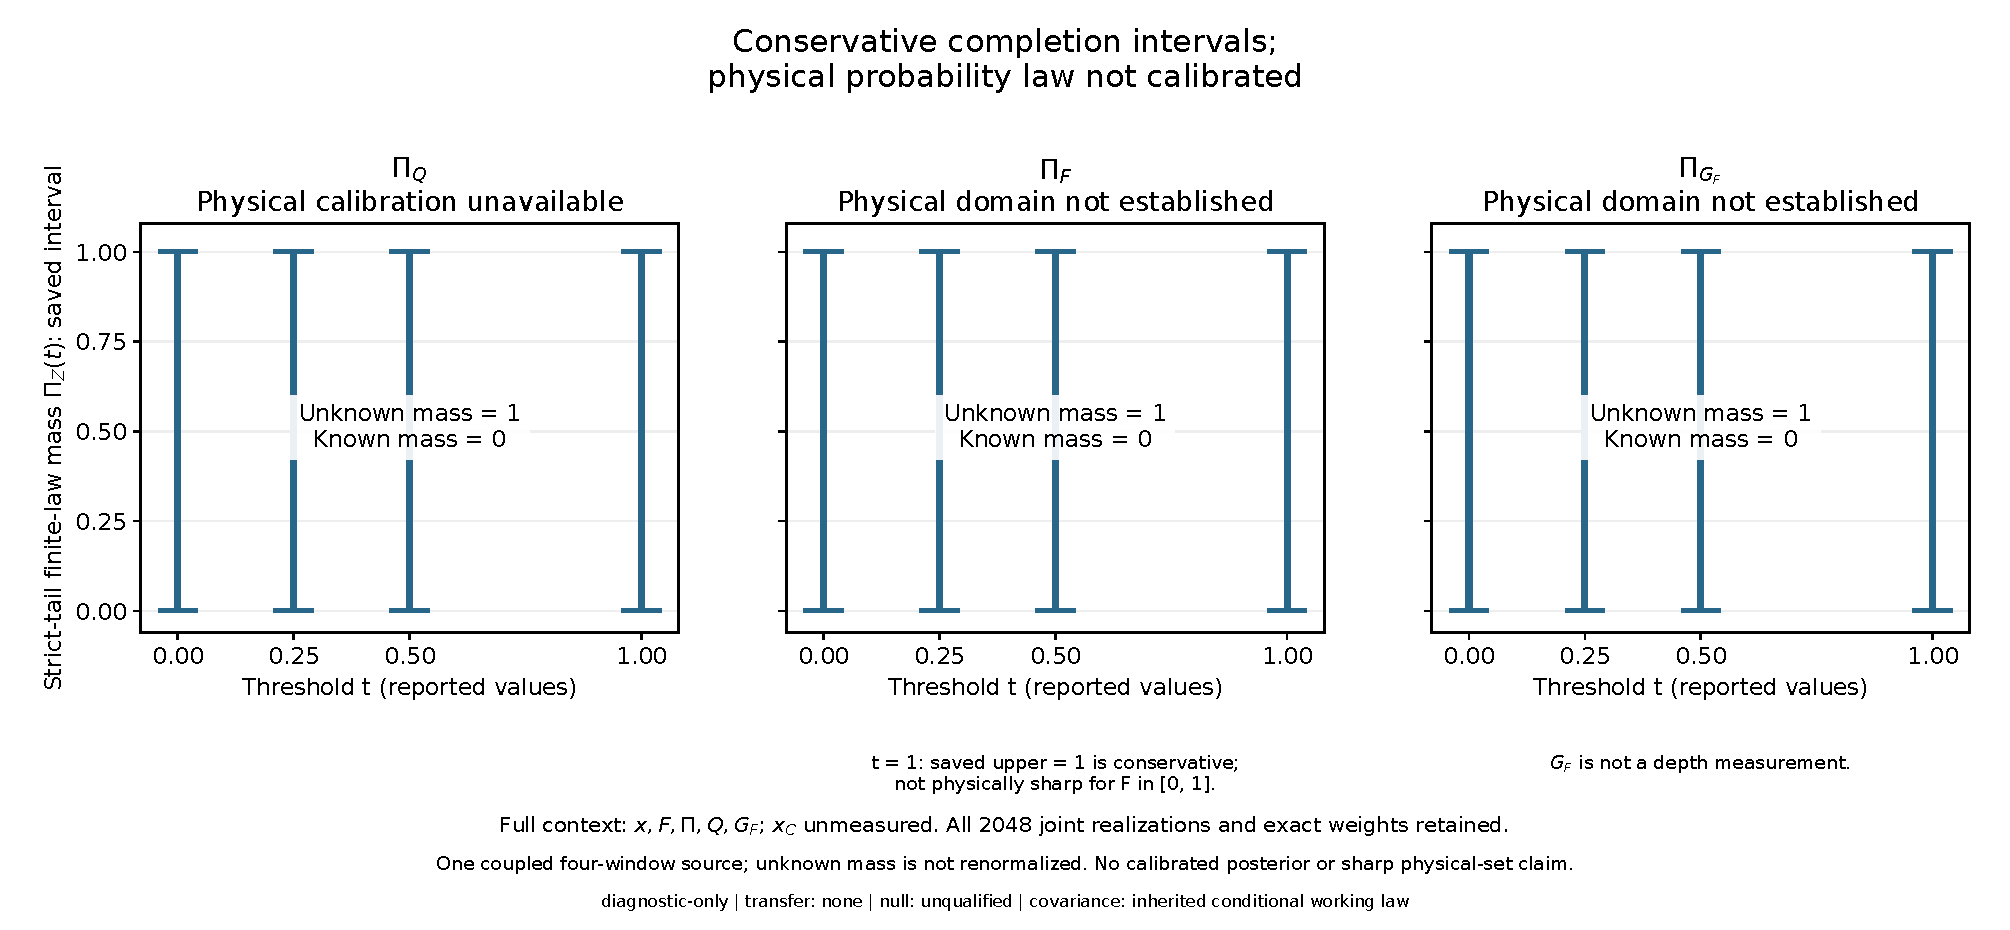
\includegraphics[width=\linewidth,height=.71\textheight,keepaspectratio]{figures/f001_external.pdf}
\caption{Conservative completion intervals for strict exceedance under the coupled 2048-point group-fit measure. Physical functions retain unknown mass one; their physical probability law is not calibrated. Zero, a threshold tie, and a function outside its domain are distinct. The displayed filling-fraction interval at threshold one is an outer completion envelope and is not asserted sharp.}
\label{fig:f001}
\end{figure}
\clearpage
\begin{figure}[p]
\centering
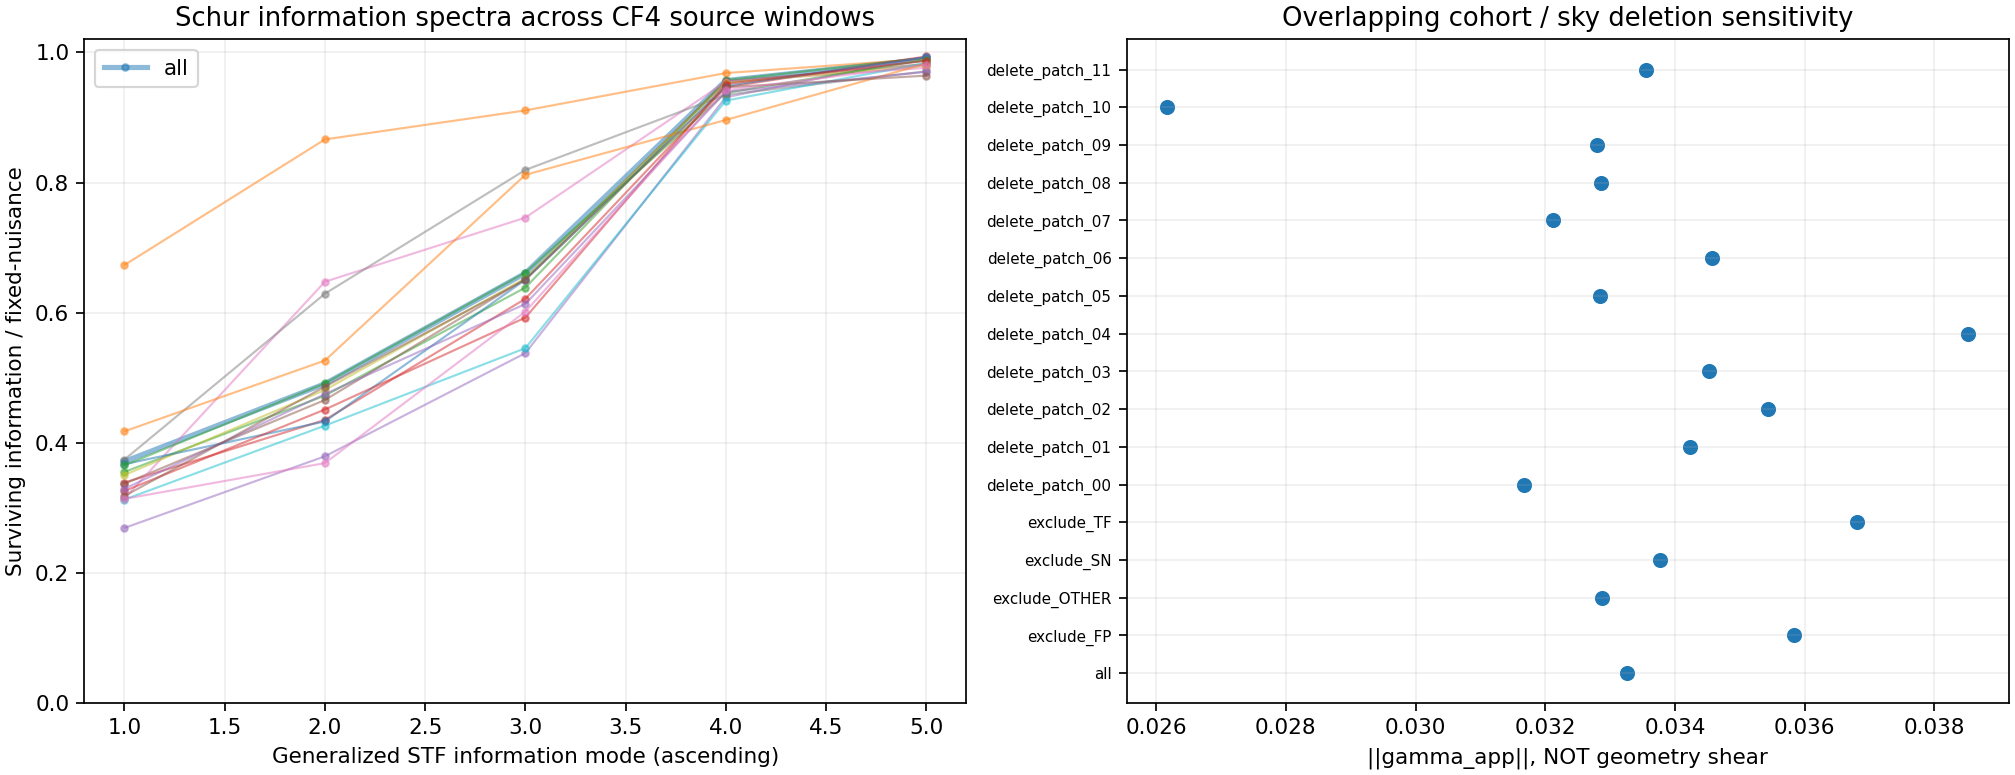
\includegraphics[width=\linewidth,height=.71\textheight,keepaspectratio]{figures/f002.png}
\caption{Conditional information for the full five-coordinate Cosmicflows STF response after nuisance profiling. Dependence assumptions change the retained information. The fit uses a fixed source-conditioned Gaussian design; these information and sensitivity summaries are not physical shear constraints.}
\label{fig:f002}
\end{figure}
\clearpage
\begin{figure}[p]
\centering
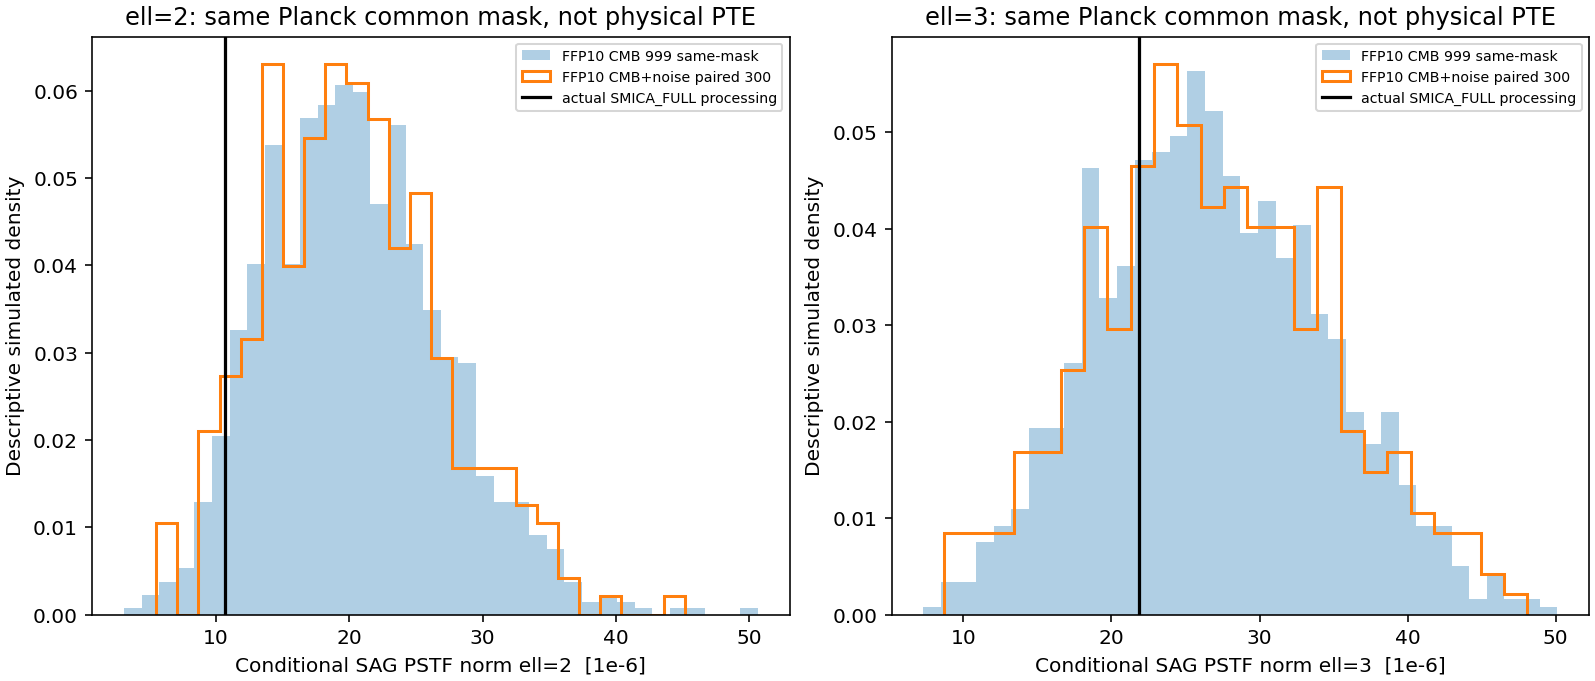
\includegraphics[width=\linewidth,height=.71\textheight,keepaspectratio]{figures/f004.png}
\caption{Low-multipole normalization and mask effects in retained Planck source simulations. The angular moments and finite mask response are evaluated with their stated tensor convention. One observed sky and fixed-weight simulations do not supply the all-observer derivative assumptions required for a physical near-isotropy bound.}
\label{fig:f004}
\end{figure}
\clearpage
\begin{figure}[p]
\centering
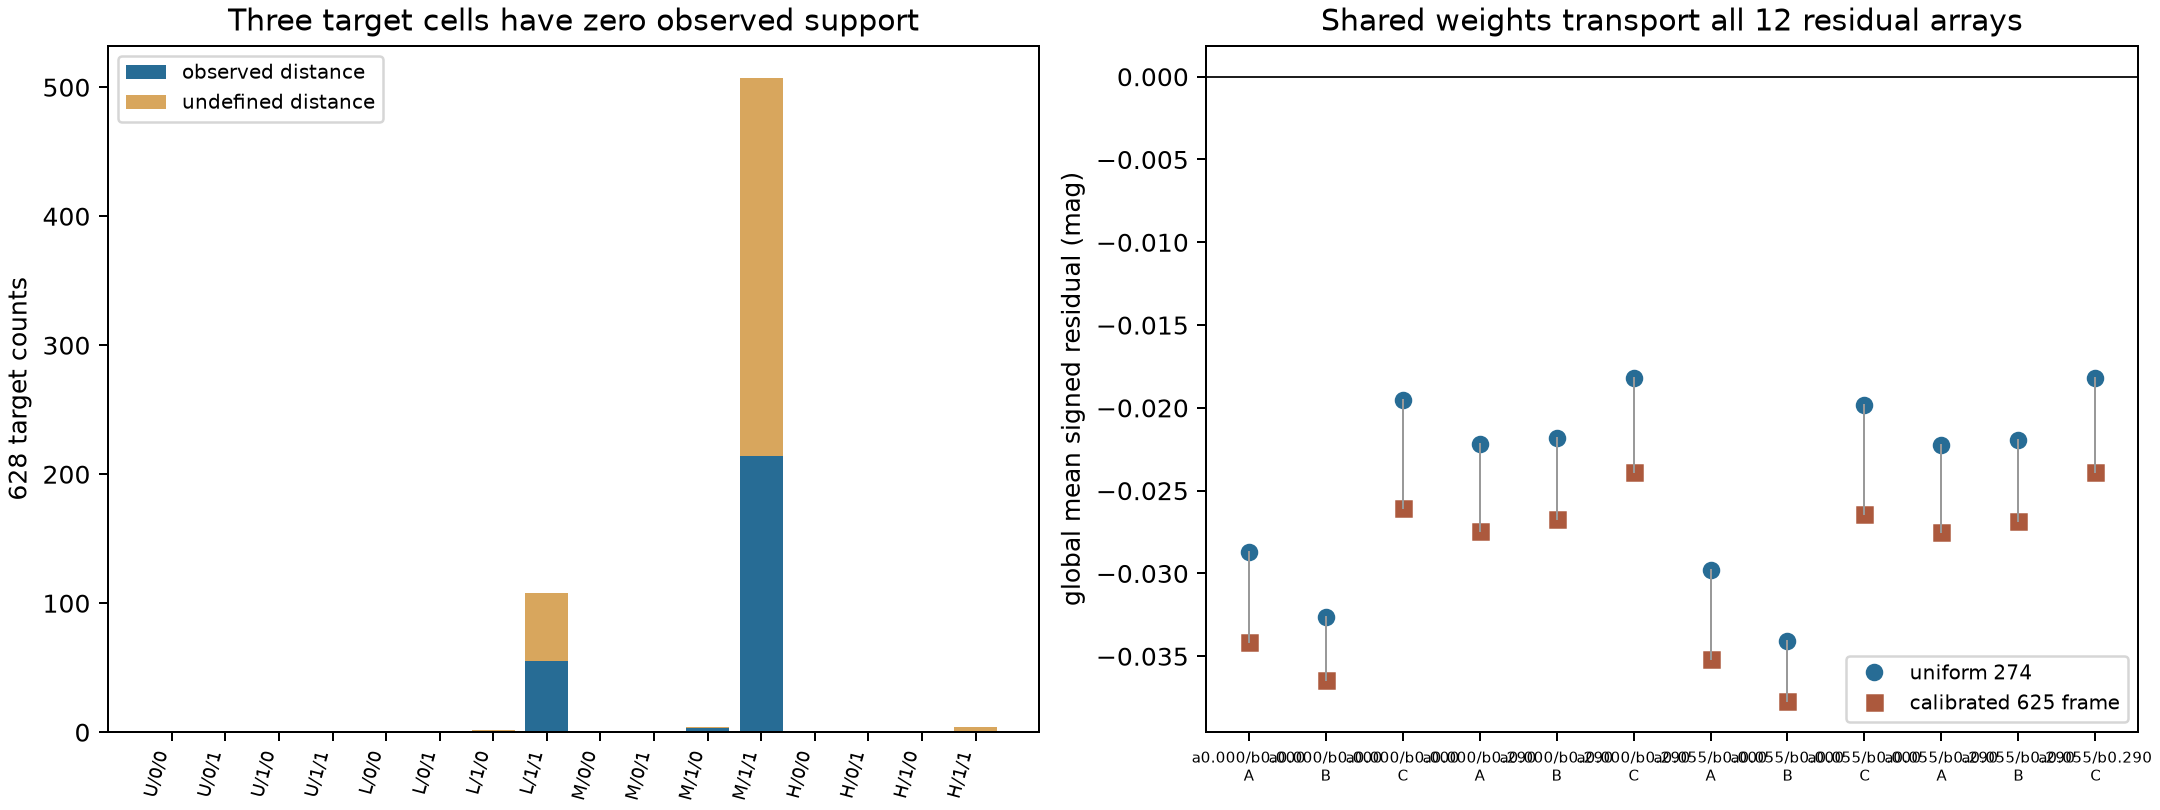
\includegraphics[width=\linewidth,height=.71\textheight,keepaspectratio]{figures/f005.png}
\caption{Auxiliary support and calibrated residual means in the incomplete distance cohort. Unsupported cells prevent exact balancing of the full target frame. Removing them changes the target; positive weights in the restricted frame do not identify missing outcomes or a physical selected-source law.}
\label{fig:f005}
\end{figure}
\clearpage
\begin{figure}[p]
\centering
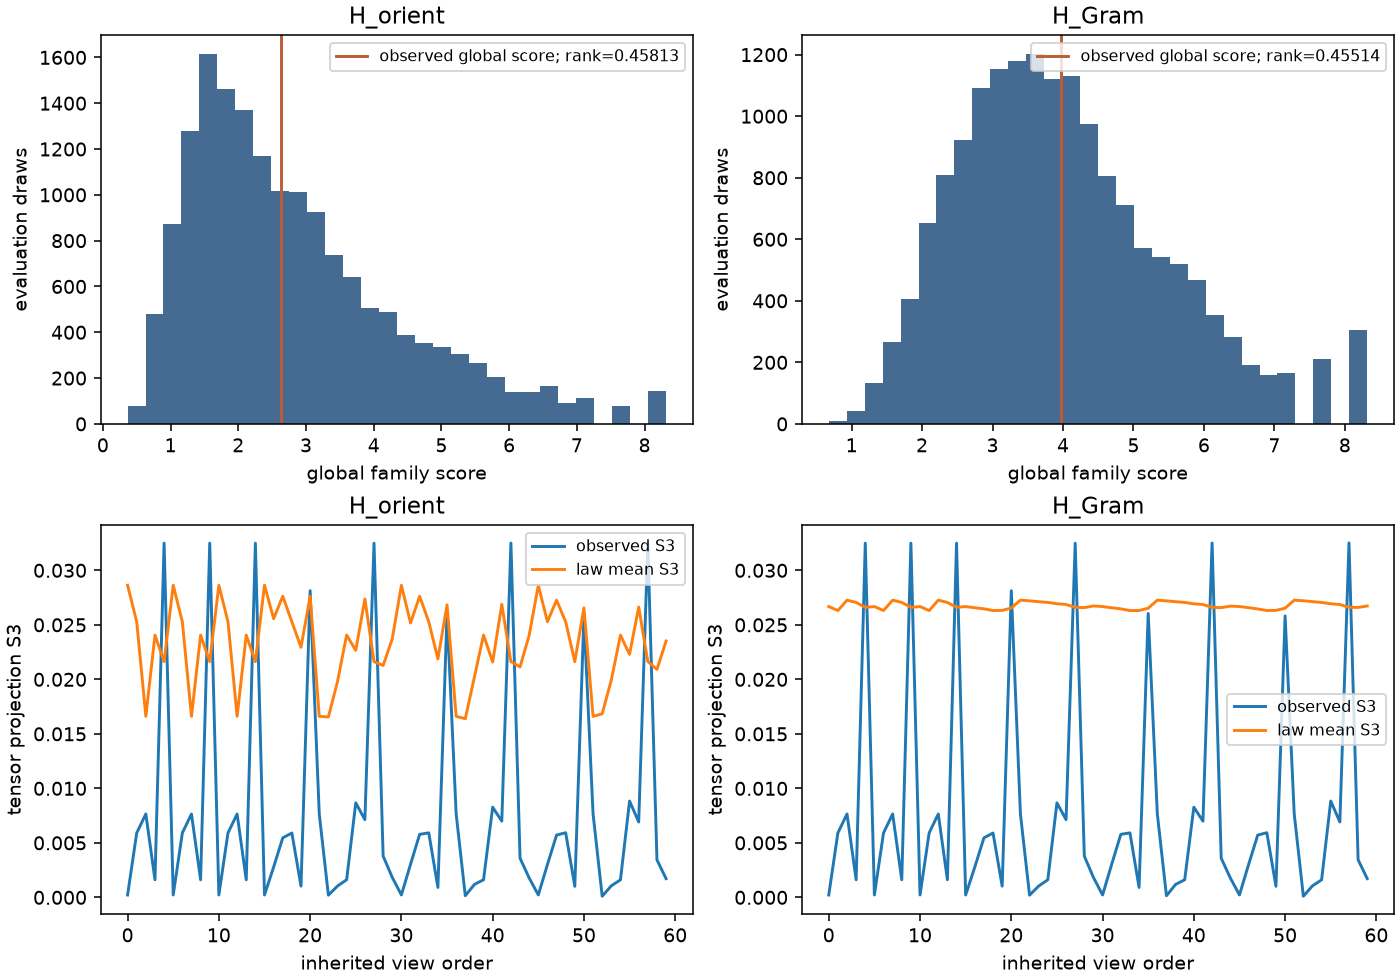
\includegraphics[width=\linewidth,height=.71\textheight,keepaspectratio]{figures/f008.png}
\caption{Constructed spatial-rotation and Gram-preserving reference laws for sixty processed E-pseudoalm views of one Planck sky. A common action preserves dependence across views. The ranks and Monte Carlo intervals refer to the named conditional laws; actual mask and foreground invariance is not established.}
\label{fig:f008}
\end{figure}
\clearpage
\begin{figure}[p]
\centering
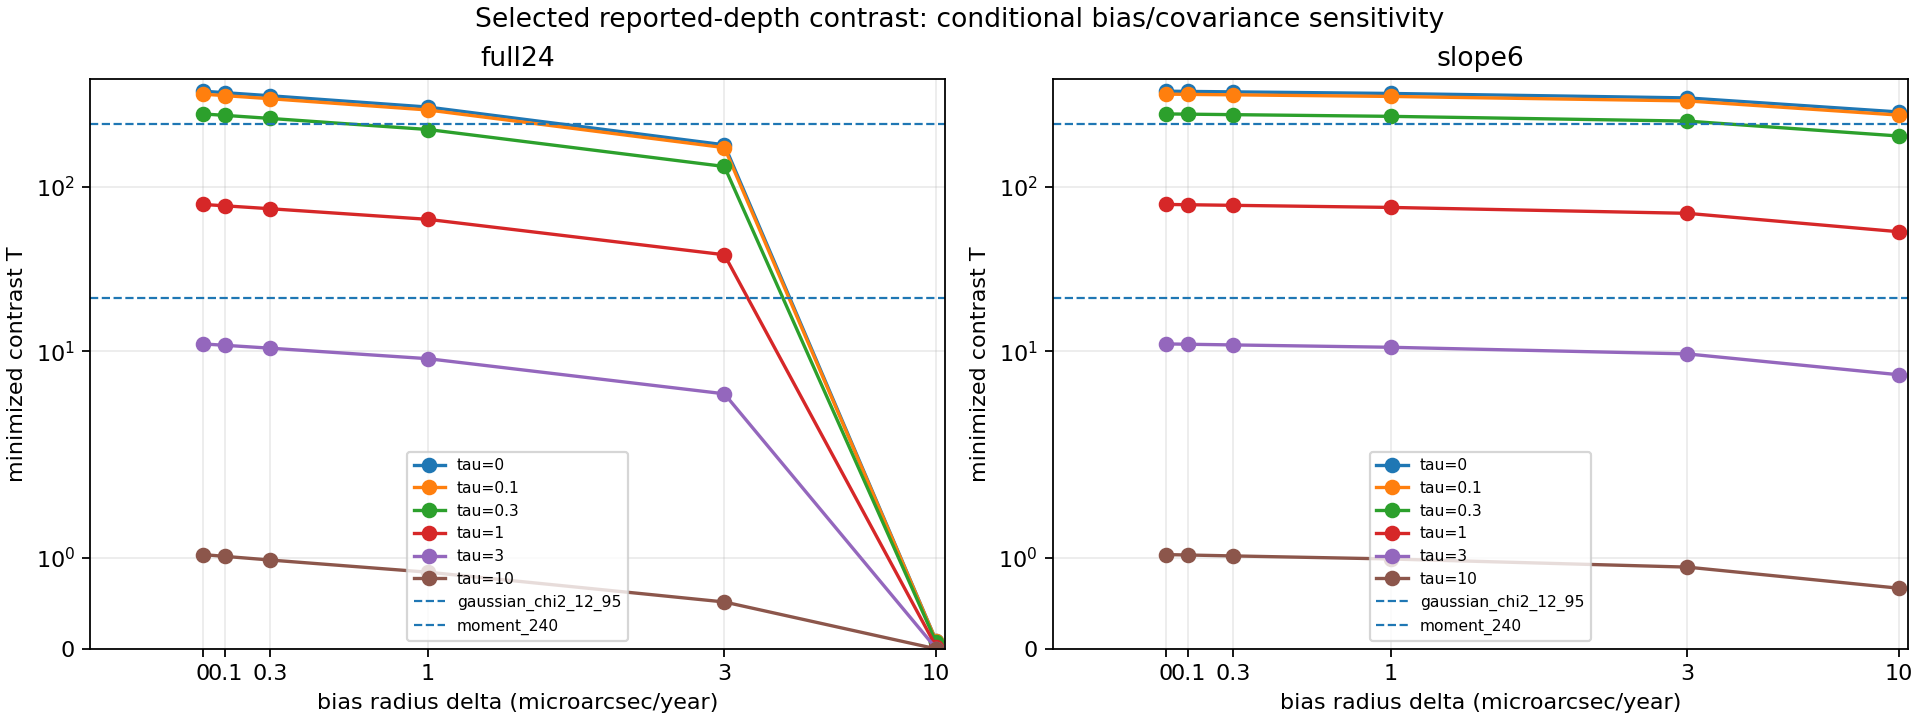
\includegraphics[width=\linewidth,height=.71\textheight,keepaspectratio]{figures/f009.png}
\caption{Conditional reported-depth bias frontier for the full astrometric state and the slope-restricted subspace. Each curve minimizes the contrast quadratic over the stated bias ball with all covariance cross blocks retained. The radii are scenarios, not measured Gaia biases or calibrated physical exclusions.}
\label{fig:f009}
\end{figure}
\clearpage
\begin{figure}[p]
\centering
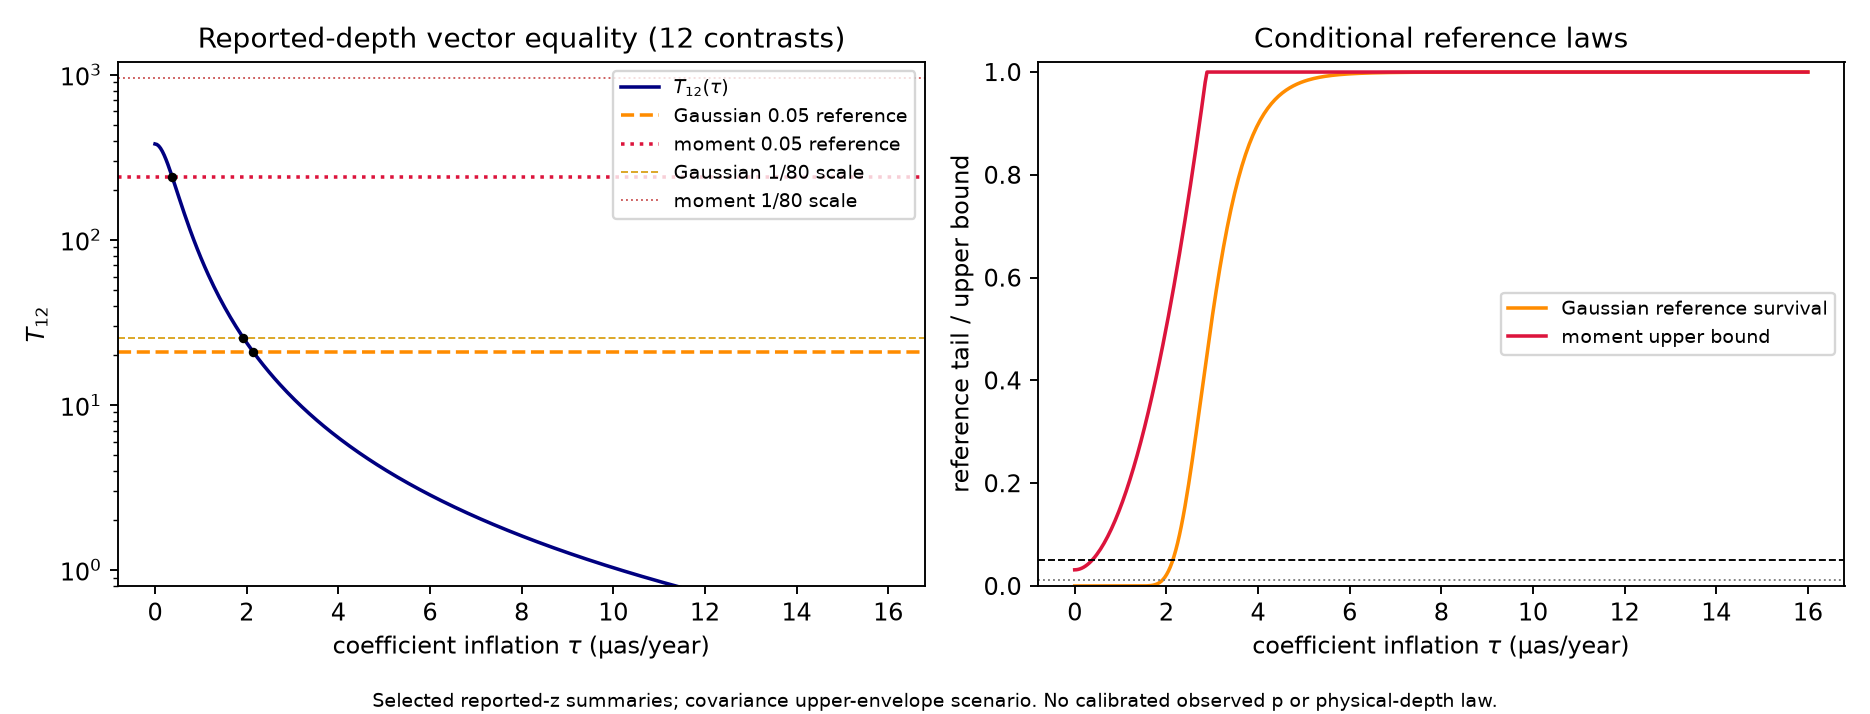
\includegraphics[width=\linewidth,height=.71\textheight,keepaspectratio]{figures/f010.png}
\caption{Reported-depth constancy under covariance inflation. The Gaussian and distribution-free moment lines require their respective mean and covariance-domination assumptions. The actual cross-source covariance is unknown, so the plotted tails and crossings are conditional sensitivity results.}
\label{fig:f010}
\end{figure}
\clearpage
\begin{figure}[p]
\centering
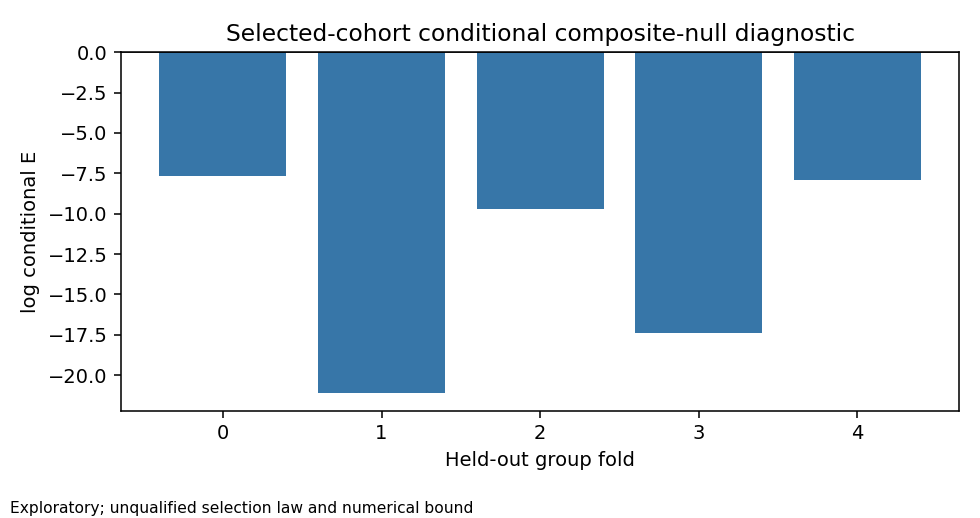
\includegraphics[width=\linewidth,height=.71\textheight,keepaspectratio]{figures/f011.png}
\caption{Conditional distance-model ratios on whole-group held-out blocks. The fixed normalized alternative mixture is compared with a composite null; dependent fold ratios are averaged rather than multiplied. Selection, adaptive choices, and numerical null-supremum qualification prevent interpreting these values as calibrated observational evidence.}
\label{fig:f011}
\end{figure}
\clearpage
\begin{figure}[p]
\centering
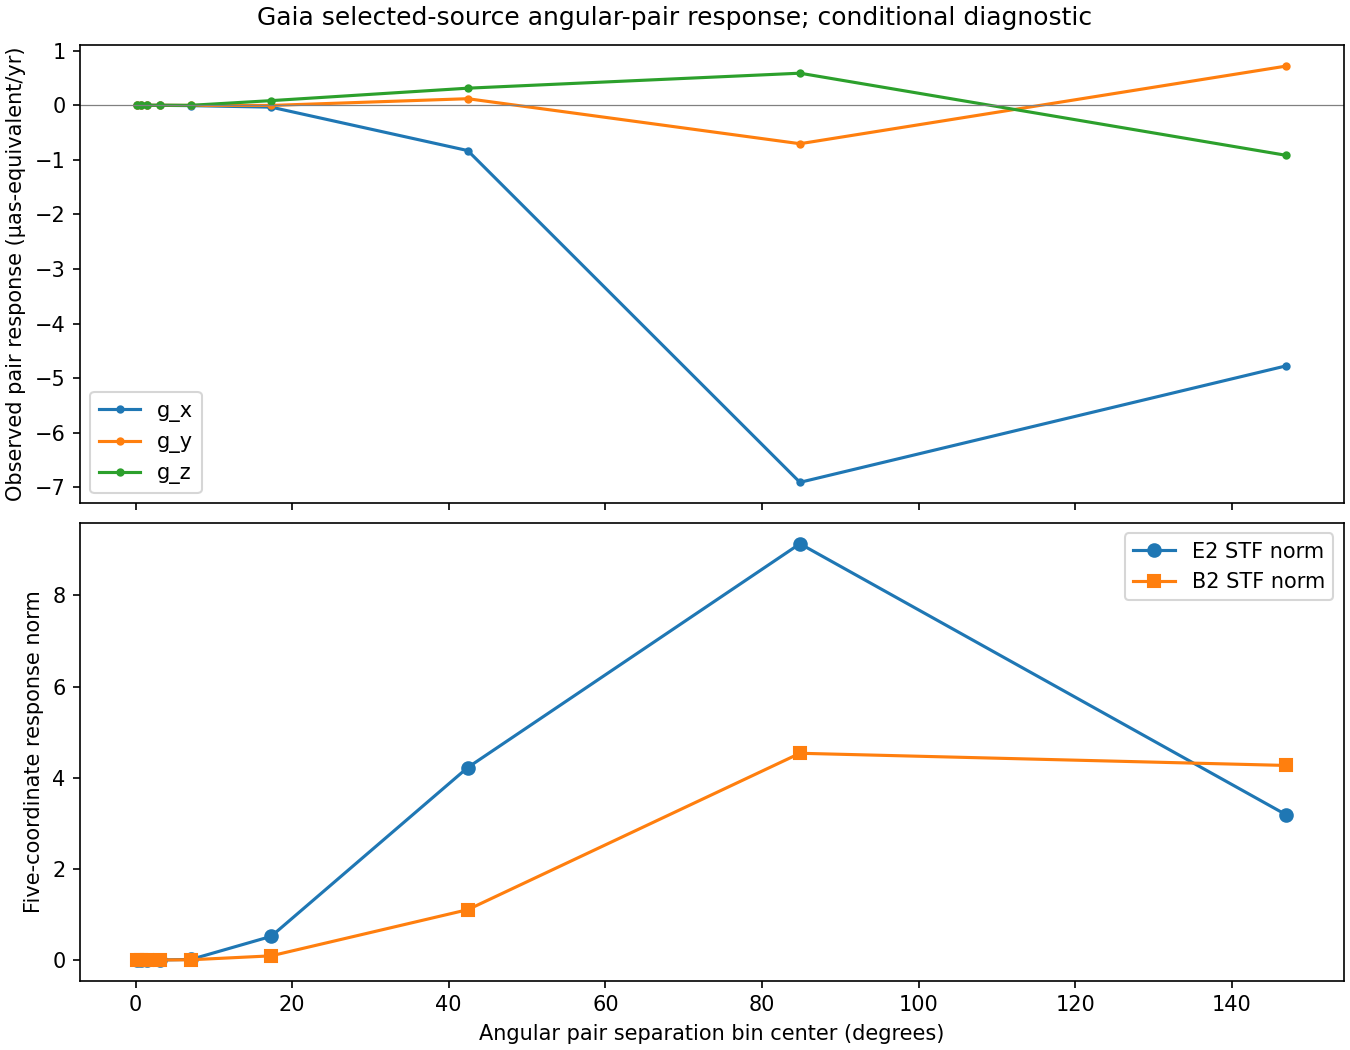
\includegraphics[width=\linewidth,height=.71\textheight,keepaspectratio]{figures/f012.png}
\caption{Angular-pair responses and representative vector/STF profiles for the retained Gaia source set. The measured response is the binned operator applied to tangent motions, not a coefficient estimate. Shared-source covariance is included; cross-source covariance and source-selection calibration are unavailable. Angular separation is not depth.}
\label{fig:f012}
\end{figure}
\clearpage
\begin{figure}[p]
\centering
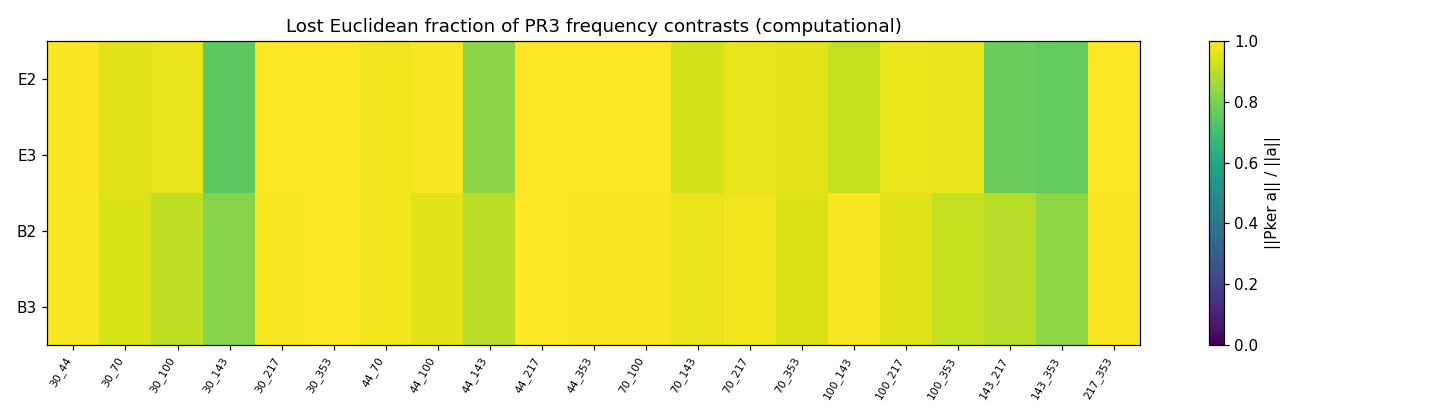
\includegraphics[width=\linewidth,height=.71\textheight,keepaspectratio]{figures/f013.png}
\caption{Spectral information lost by a single cleaned CMB map. The finite seven-channel linear compression maps 168 real harmonic coordinates to 24, with rank 24 and a 144-dimensional kernel. Frequency contrasts can lie in that kernel. This is a response-space calculation for the retained weights, not a seven-frequency sky measurement or a foreground rejection.}
\label{fig:f013}
\end{figure}
\clearpage
\begin{figure}[p]
\centering
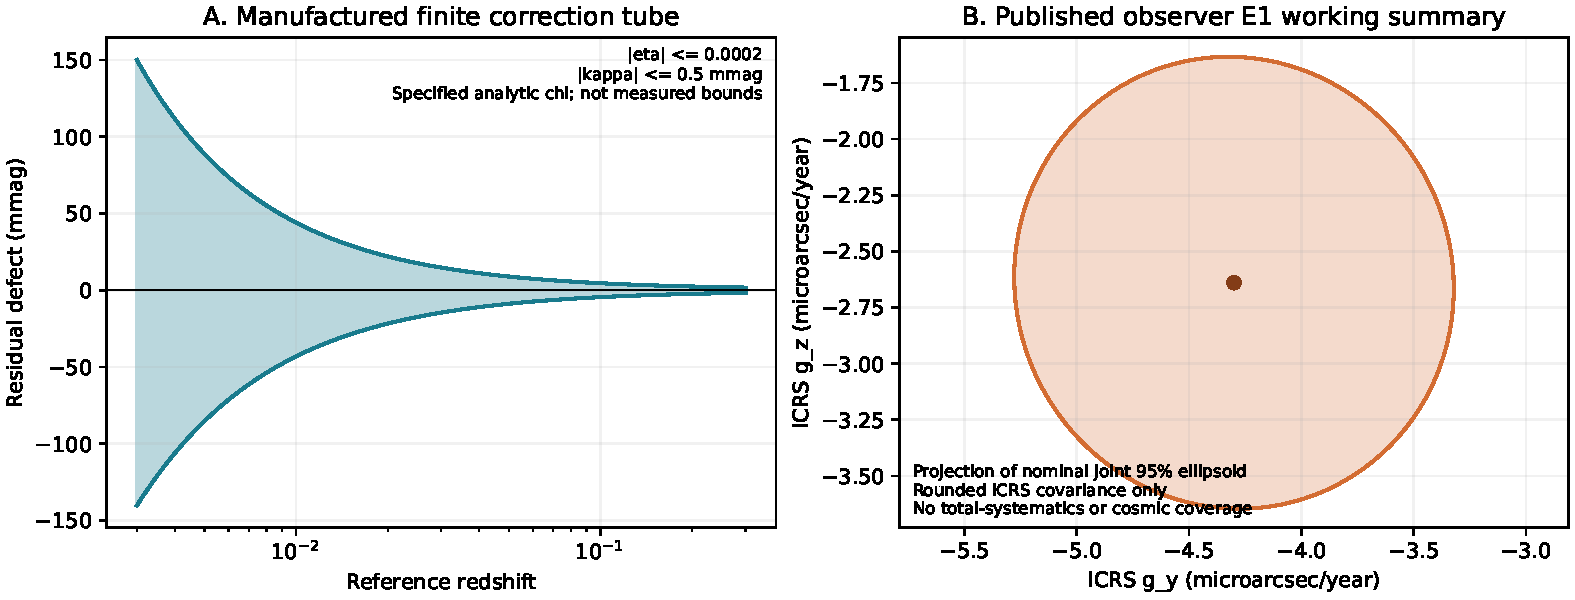
\includegraphics[width=\linewidth,height=.71\textheight,keepaspectratio]{figures/f014.pdf}
\caption{Conditional analytic and observational response comparisons. The finite response example uses declared nuisance radii; the astrometric panel uses its published observer-vector working summary. Neither an assumed radius nor an observer pattern is a measured bound on a cosmological history.}
\label{fig:f014}
\end{figure}
\clearpage
\begin{figure}[p]
\centering
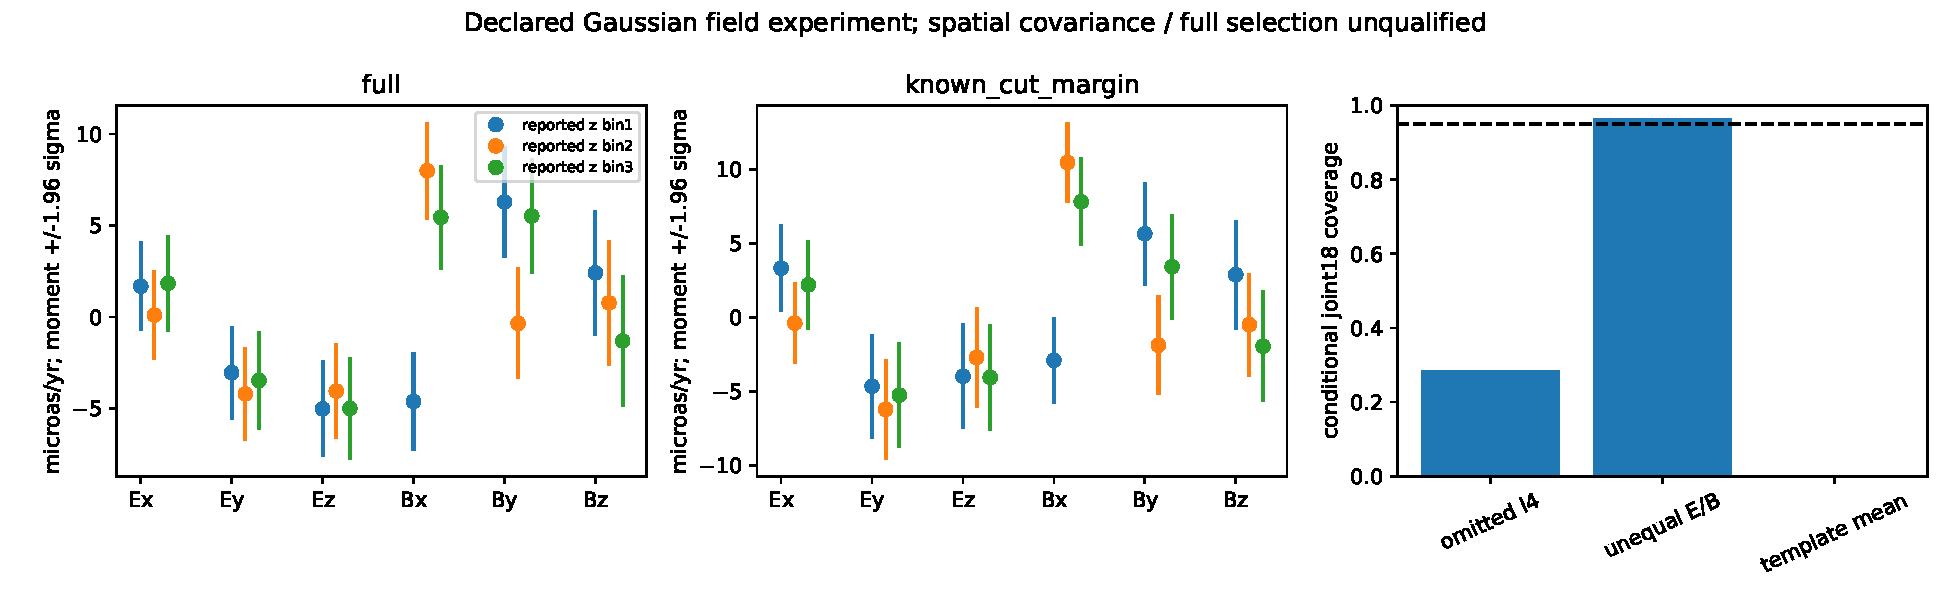
\includegraphics[width=\linewidth,height=.71\textheight,keepaspectratio]{figures/f015_external.pdf}
\caption{Reported-redshift astrometric vectors and simulated joint-coverage checks. The error bars use the stated working source covariance. Omitted high-order angular structure and template-correlated means can invalidate that coverage. Spatial covariance, full selection, true-depth response, and physical source motion remain unqualified.}
\label{fig:f015}
\end{figure}
\clearpage
\begin{figure}[p]
\centering
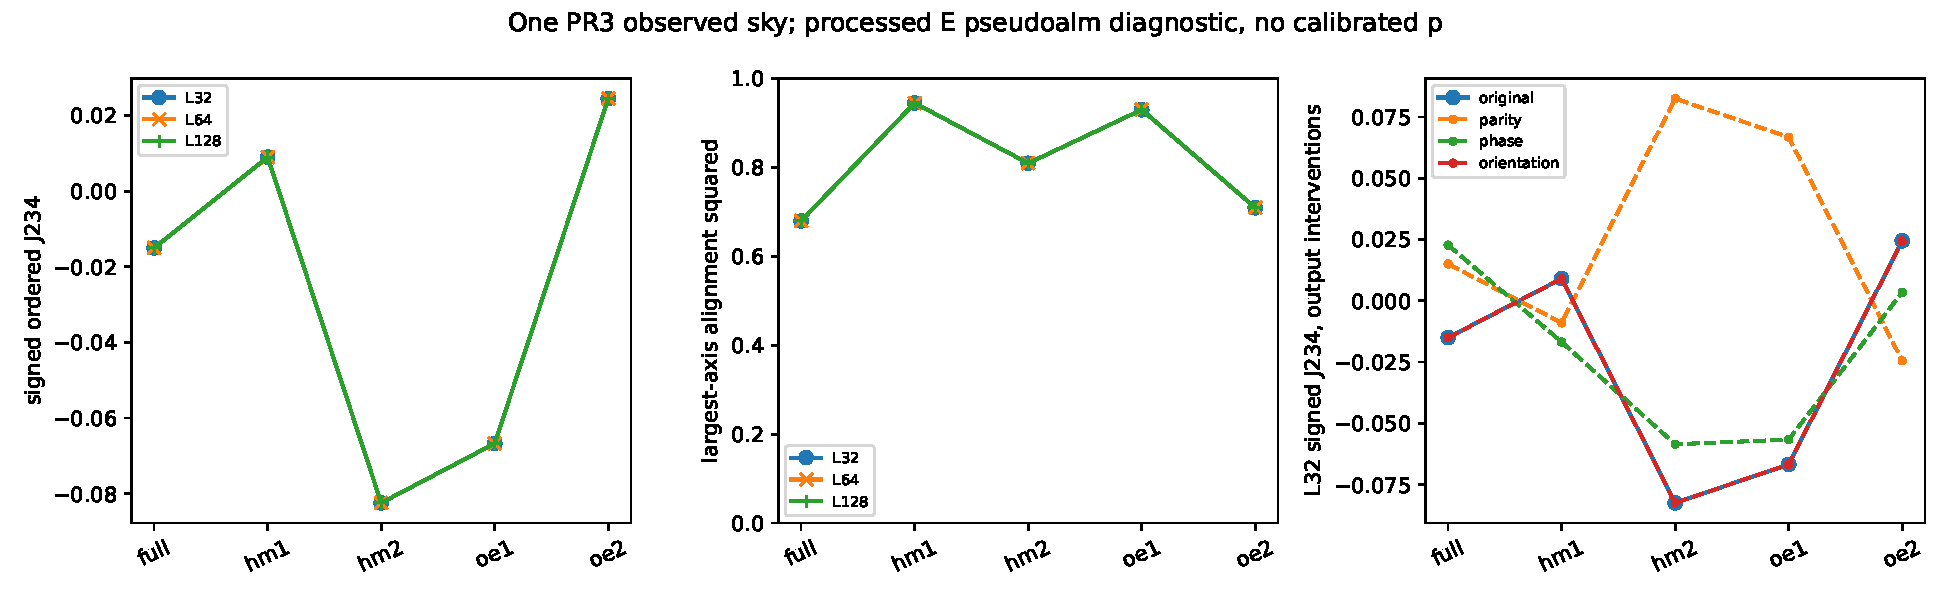
\includegraphics[width=\linewidth,height=.71\textheight,keepaspectratio]{figures/f016.pdf}
\caption{Counterpairs of processed Planck E morphology with signed contraction and axis summaries. These interventions on one observed sky demonstrate that the chosen summaries retain different information. They are retrospective processing comparisons without a calibrated physical null.}
\label{fig:f016}
\end{figure}
\clearpage
\begin{figure}[p]
\centering
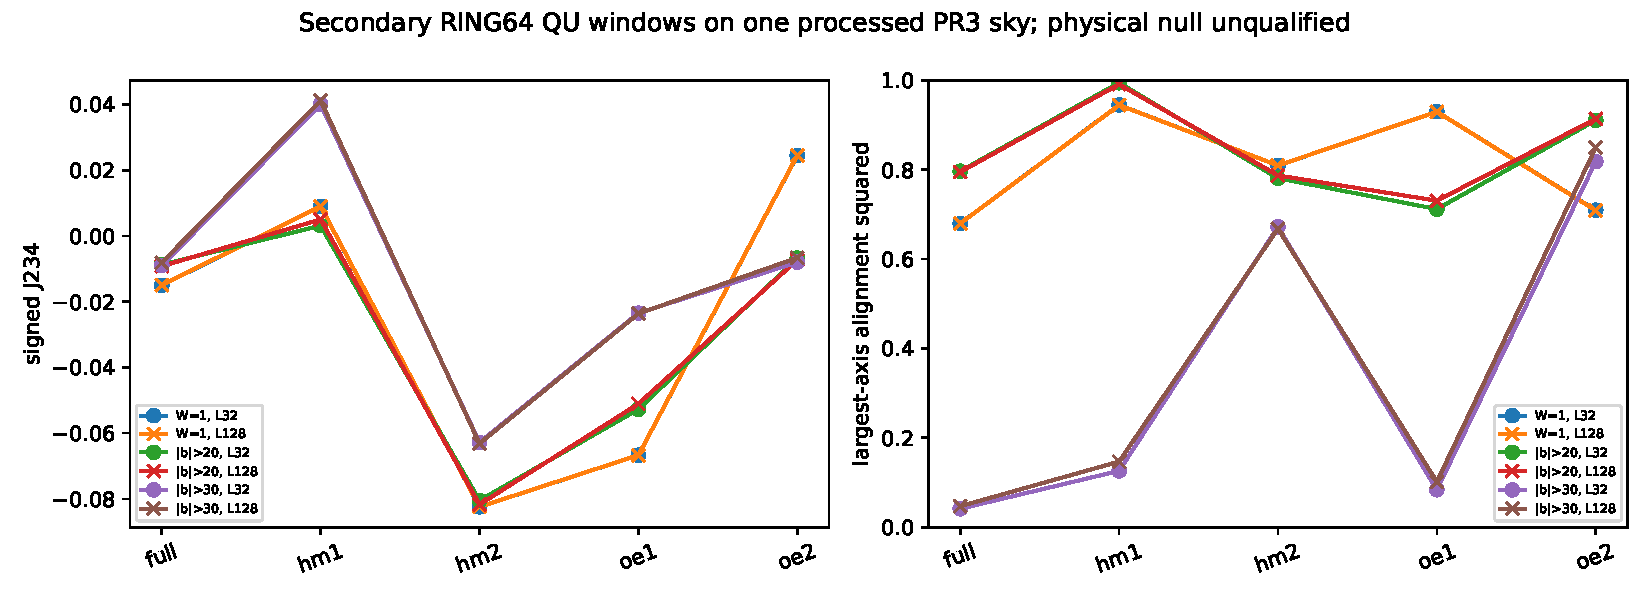
\includegraphics[width=\linewidth,height=.71\textheight,keepaspectratio]{figures/f017_external.pdf}
\caption{Secondary selected-sky windows applied to delivered Planck Q/U on one processed sky. Changes in the signed descriptor and axis alignment expose processing dependence. The windows and multipole cutoffs do not form independent sky realizations, and the physical total-field null is not calibrated.}
\label{fig:f017}
\end{figure}
\clearpage
\begin{figure}[p]
\centering
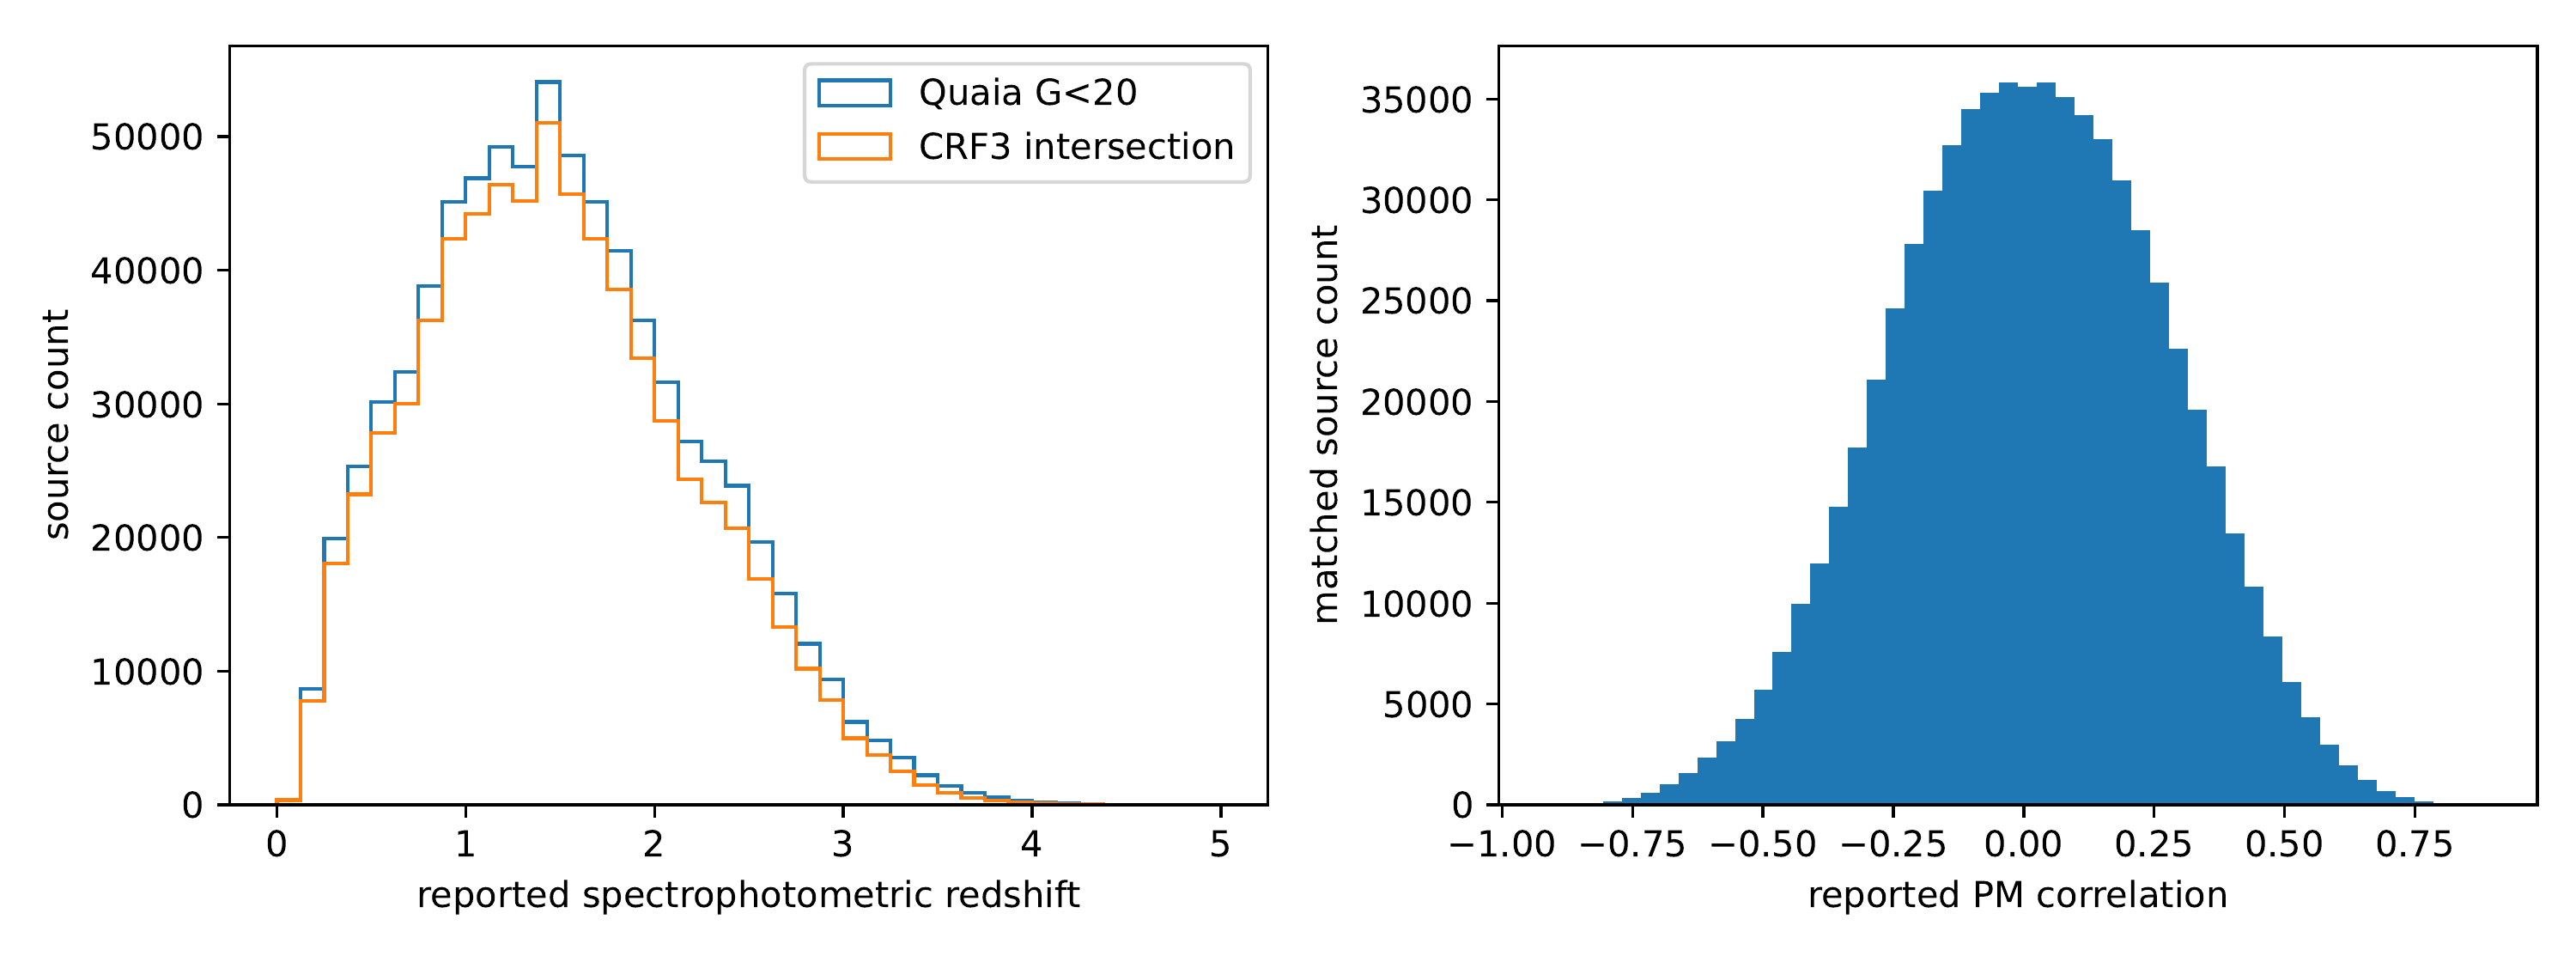
\includegraphics[width=\linewidth,height=.71\textheight,keepaspectratio]{figures/f018_external.png}
\caption{Exact-identity linkage of the selected Quaia and Gaia samples before the later supplement. The displayed redshift and match distributions describe catalogue membership. They do not measure acceleration, certify true distances, or supply a centroid-to-matter response.}
\label{fig:f018}
\end{figure}
\clearpage
\begin{figure}[p]
\centering
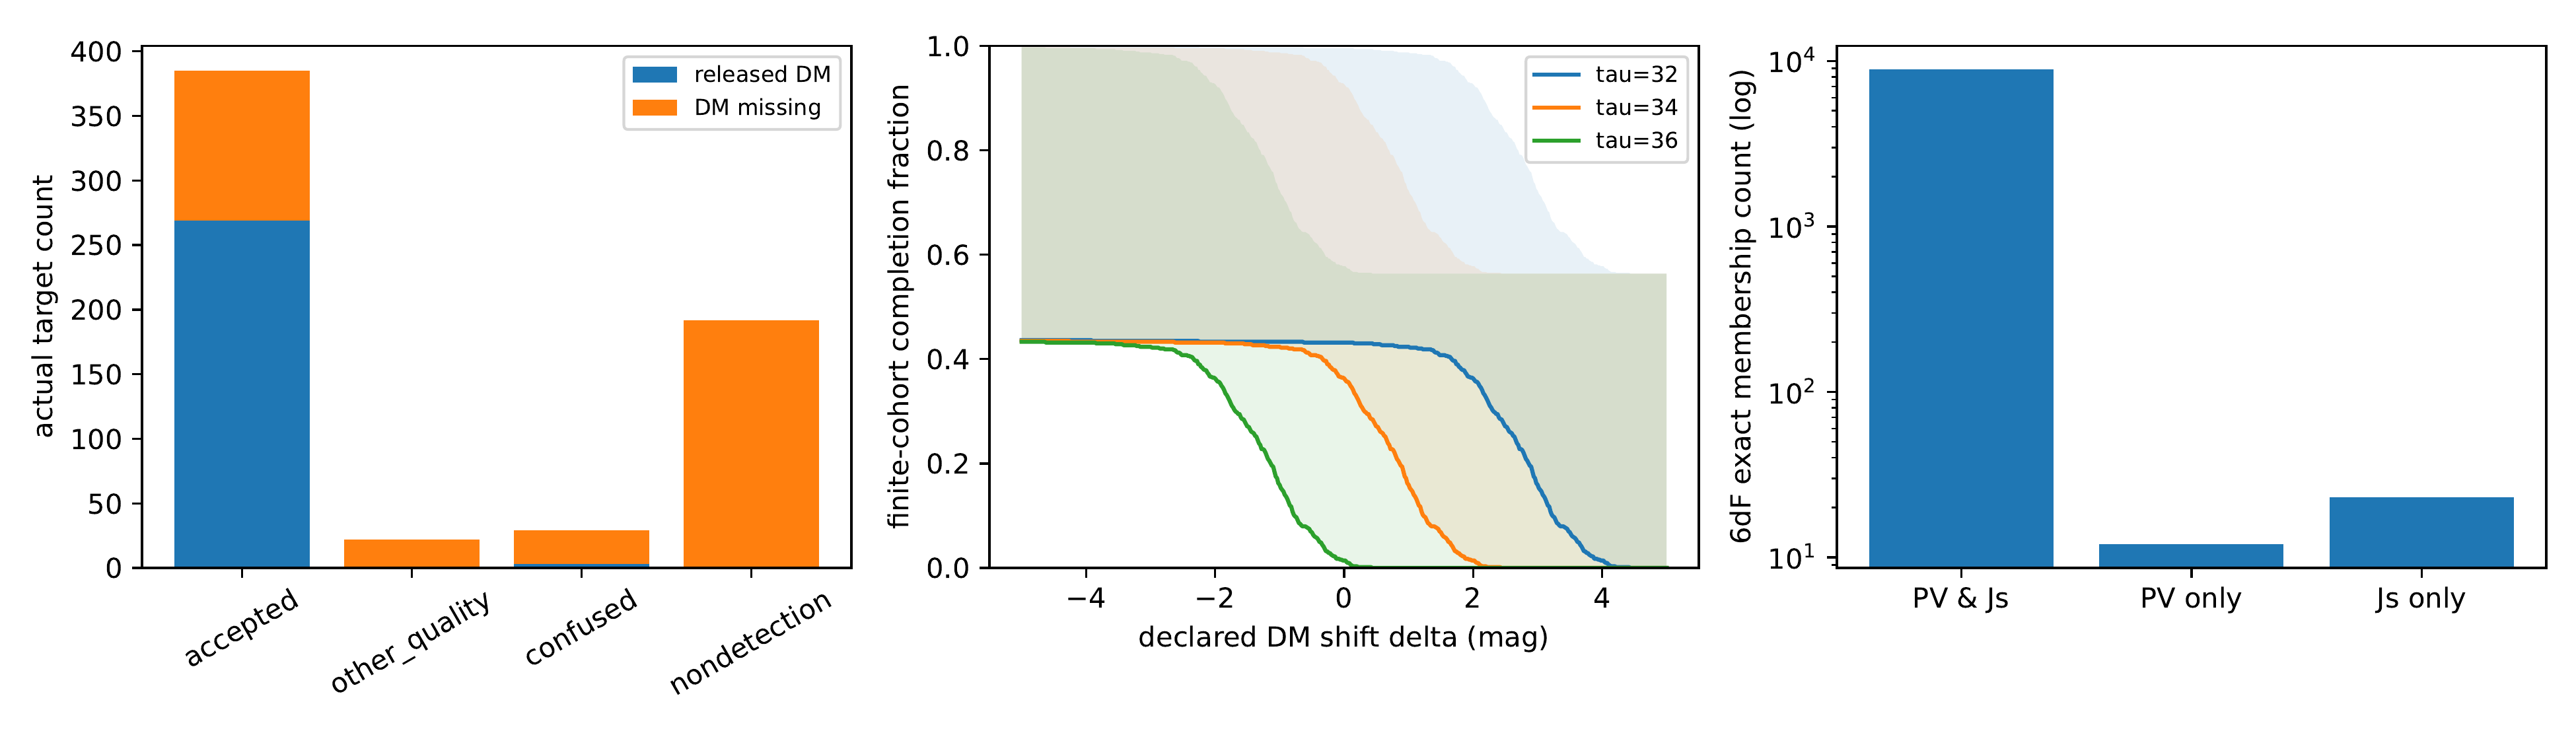
\includegraphics[width=\linewidth,height=.71\textheight,keepaspectratio]{figures/f019_external.png}
\caption{Observed outcome marks and declared missing-modulus completions in the selected distance cohort. The completion curves are conditional sensitivity models. They do not estimate the parent inclusion probability or establish the physical law of missing outcomes.}
\label{fig:f019}
\end{figure}
\clearpage
\begin{figure}[p]
\centering
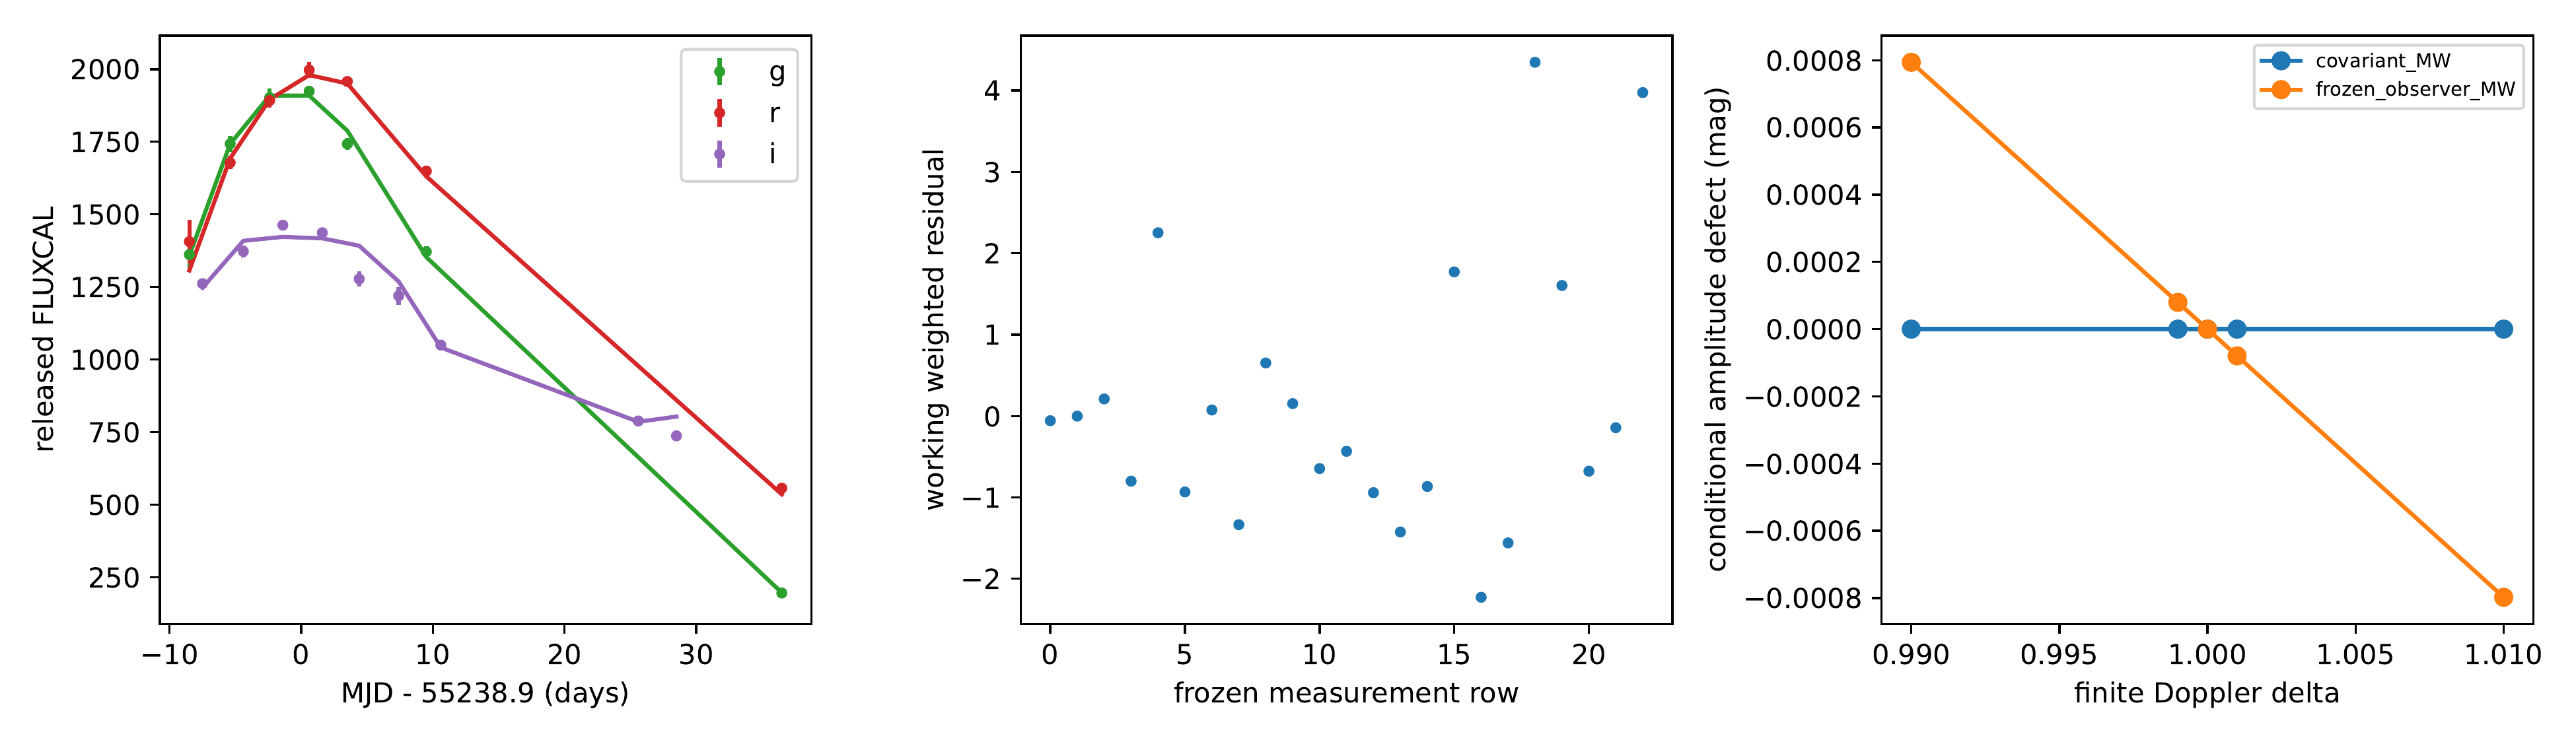
\includegraphics[width=\linewidth,height=.71\textheight,keepaspectratio]{figures/f020_external.png}
\caption{The retained SN010010 light curve, measurement-only residuals, and conditional amplitude response. The baseline fails its stated adequacy screen, and the nominal producer fit is not reproduced. This earlier diagnostic is retained to show the actual failure; the later public model-covariance calculation addresses a different question.}
\label{fig:f020}
\end{figure}
\clearpage
\begin{figure}[p]
\centering
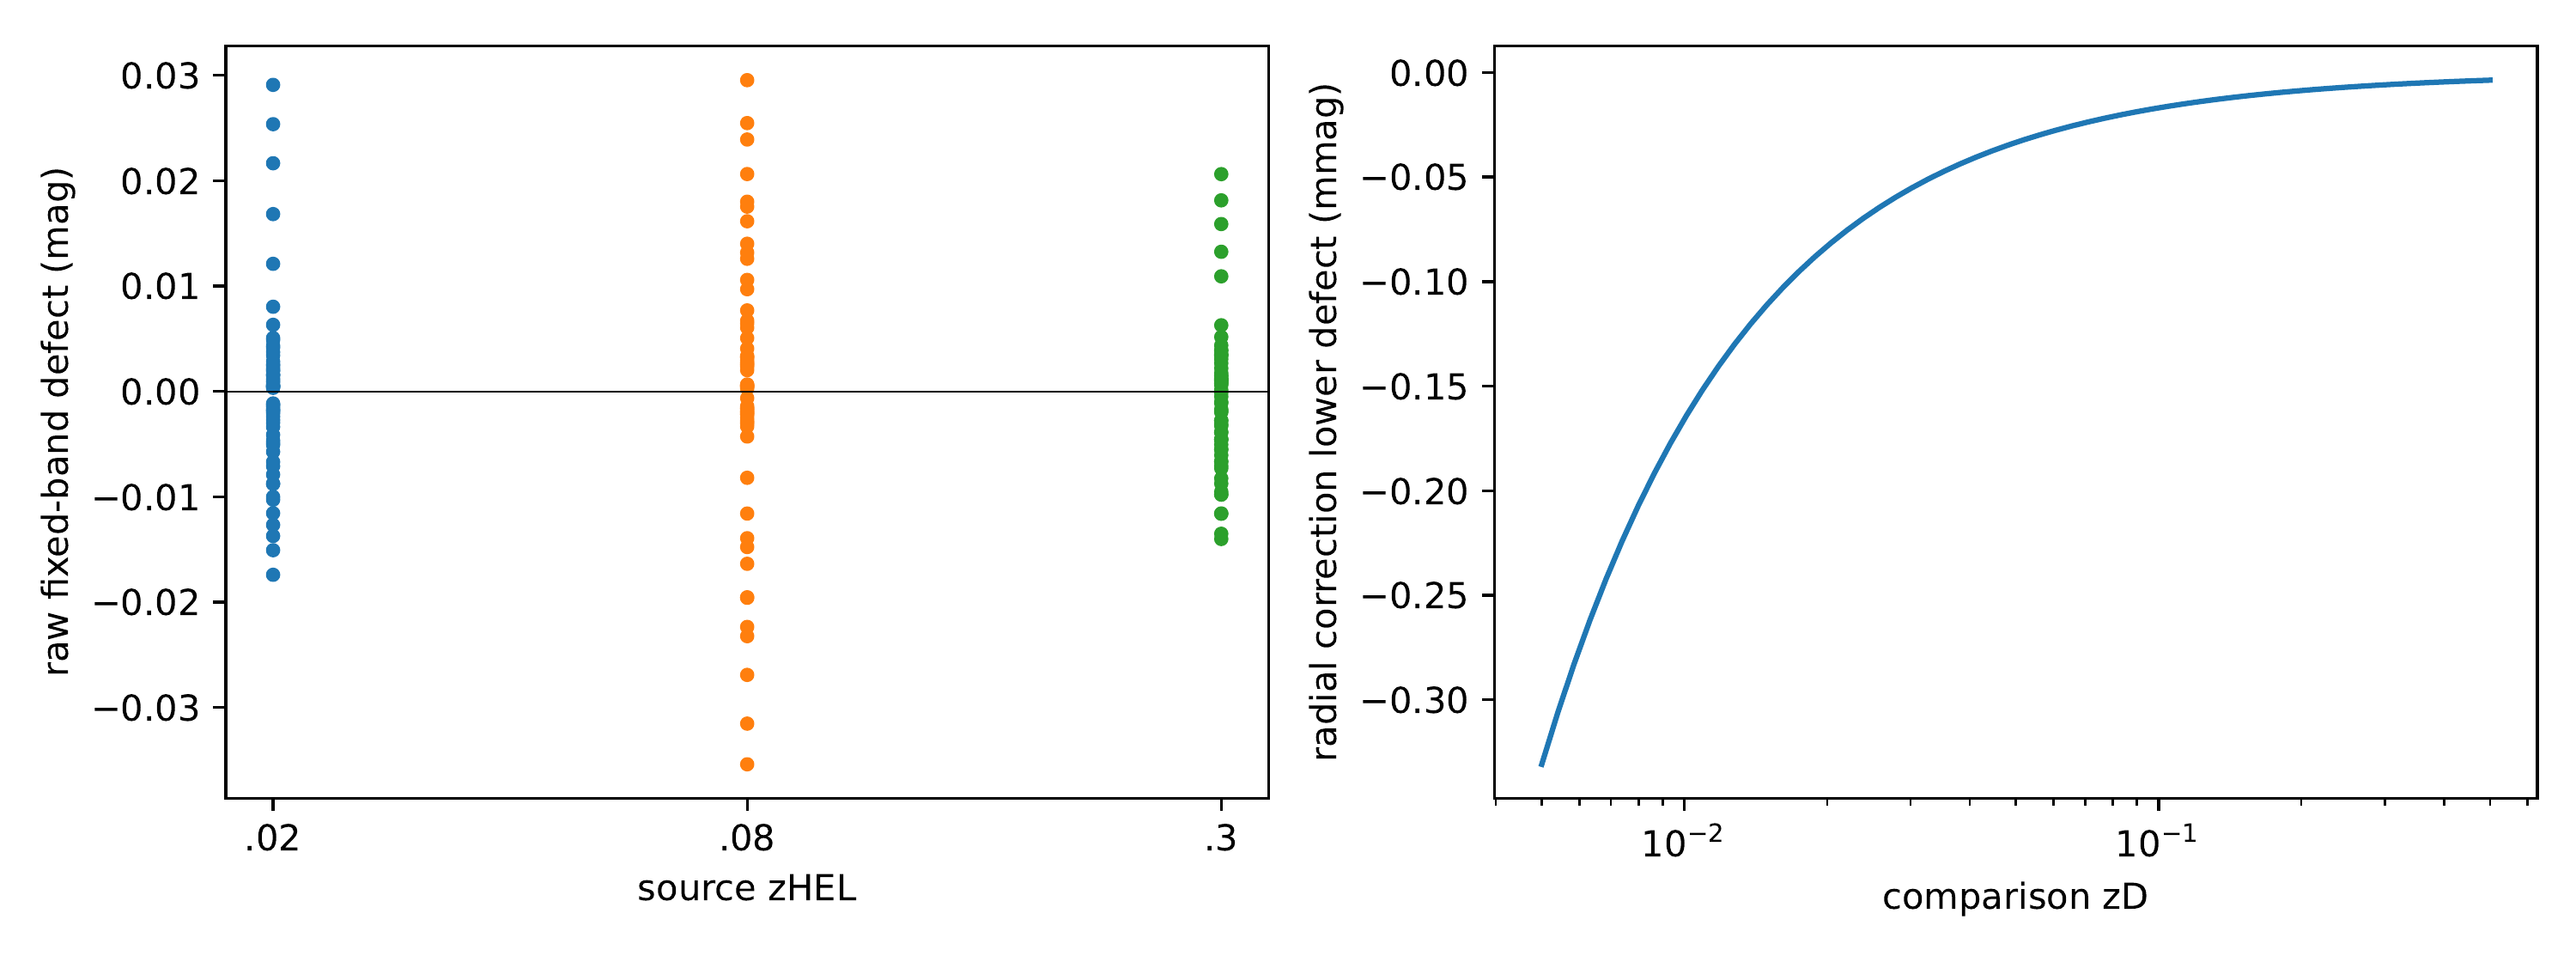
\includegraphics[width=\linewidth,height=.71\textheight,keepaspectratio]{figures/f021_external.png}
\caption{Finite spectral-refit and conditional radial-correction responses at separately specified source redshifts. A finite source calculation is not an empirical total observer-reboost correction. The nominal fitting, calibration, selection, and physical propagation responses remain additional inputs.}
\label{fig:f021}
\end{figure}
\clearpage
\begin{figure}[p]
\centering
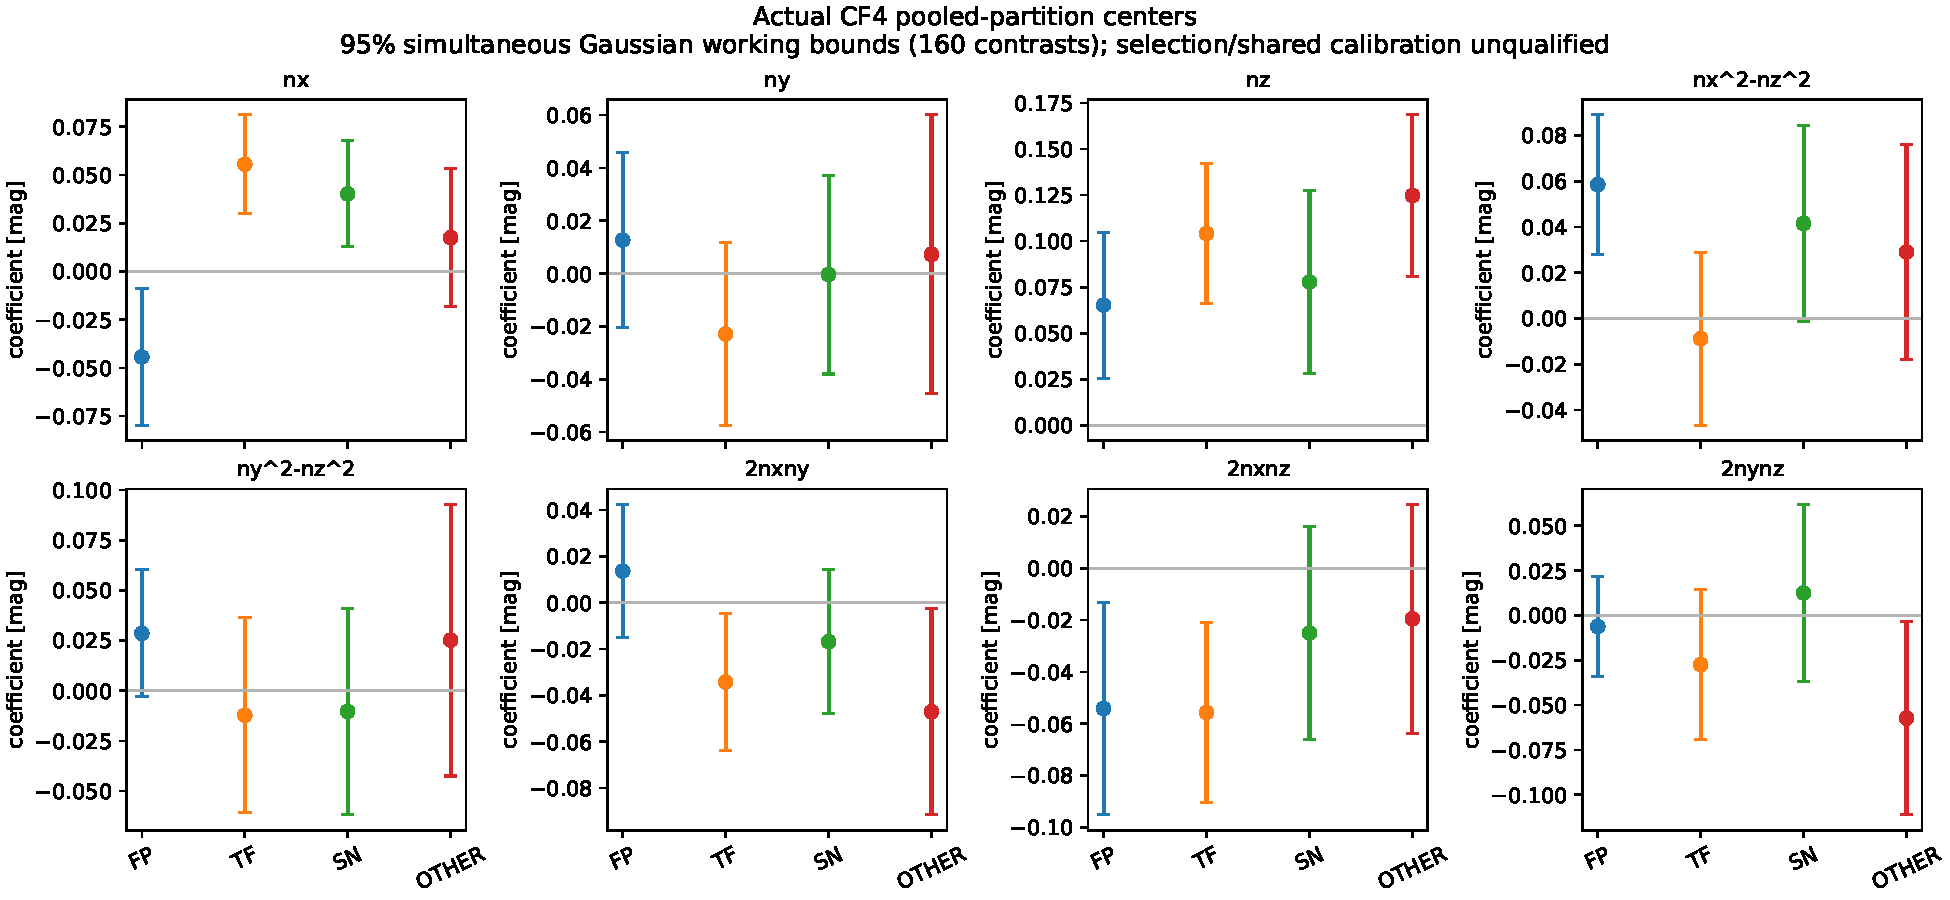
\includegraphics[width=\linewidth,height=.71\textheight,keepaspectratio]{figures/f022_external.pdf}
\caption{Observed method-dependent calibration contrasts on the retained Cosmicflows group geometry. These fitted centres supplement radius-only sensitivity calculations. Shared sources and calibration gauges remain, so method columns cannot be treated as independent physical measurements.}
\label{fig:f022}
\end{figure}
\clearpage
\begin{figure}[p]
\centering
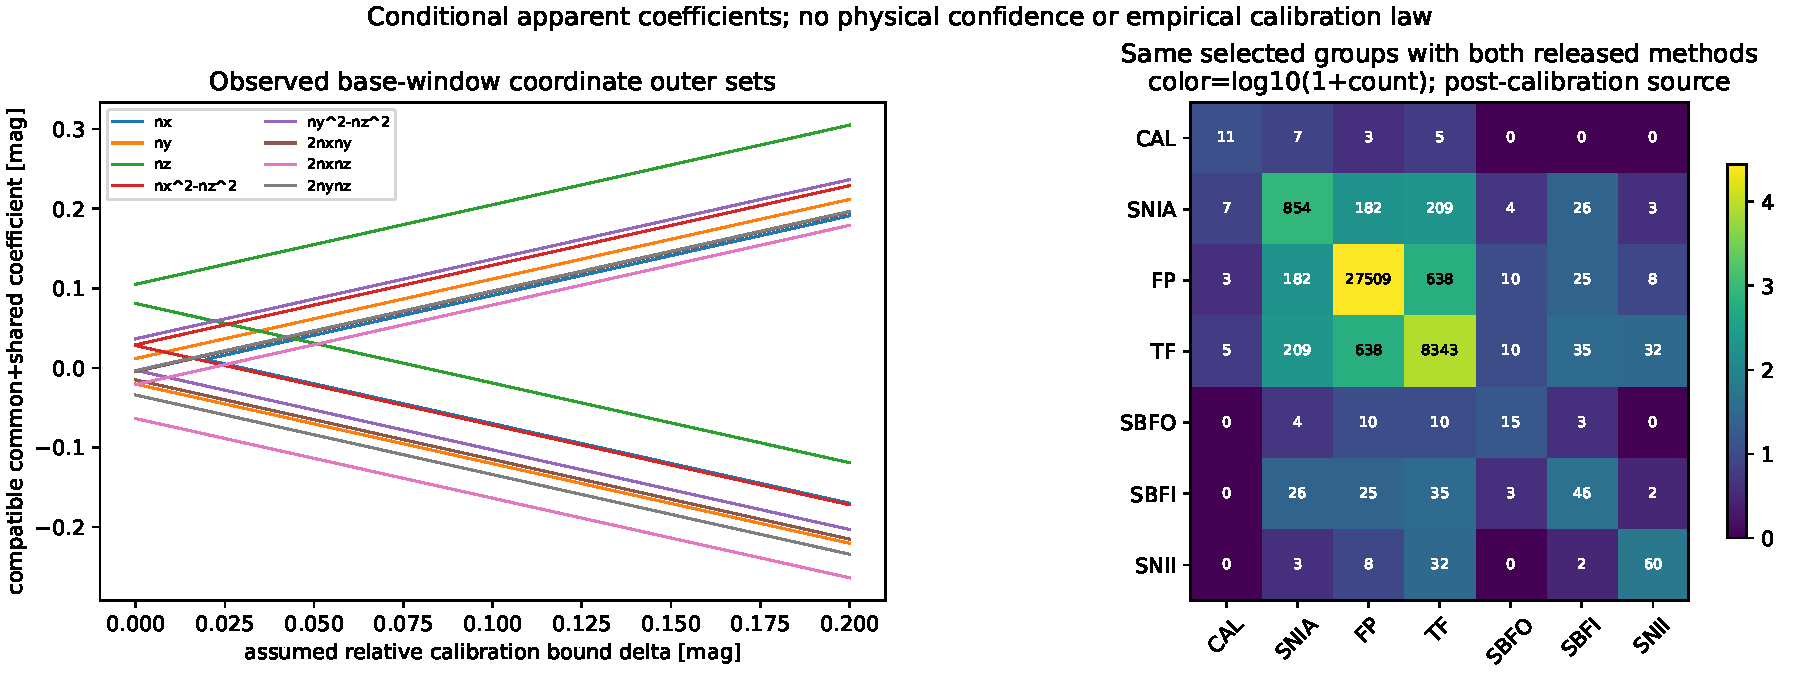
\includegraphics[width=\linewidth,height=.71\textheight,keepaspectratio]{figures/f023_external.pdf}
\caption{Apparent-coordinate outer sets as the allowed common-calibration radius increases (left), and overlap of released distance-method memberships (right). Common calibration and shared group membership affect different parts of the identification problem. These outer sets depend on the stated radius and working source summaries; the overlap does not supply independent likelihood factors or the accepted-subsource selection law.}
\label{fig:f023}
\end{figure}
\clearpage
\begin{figure}[p]
\centering
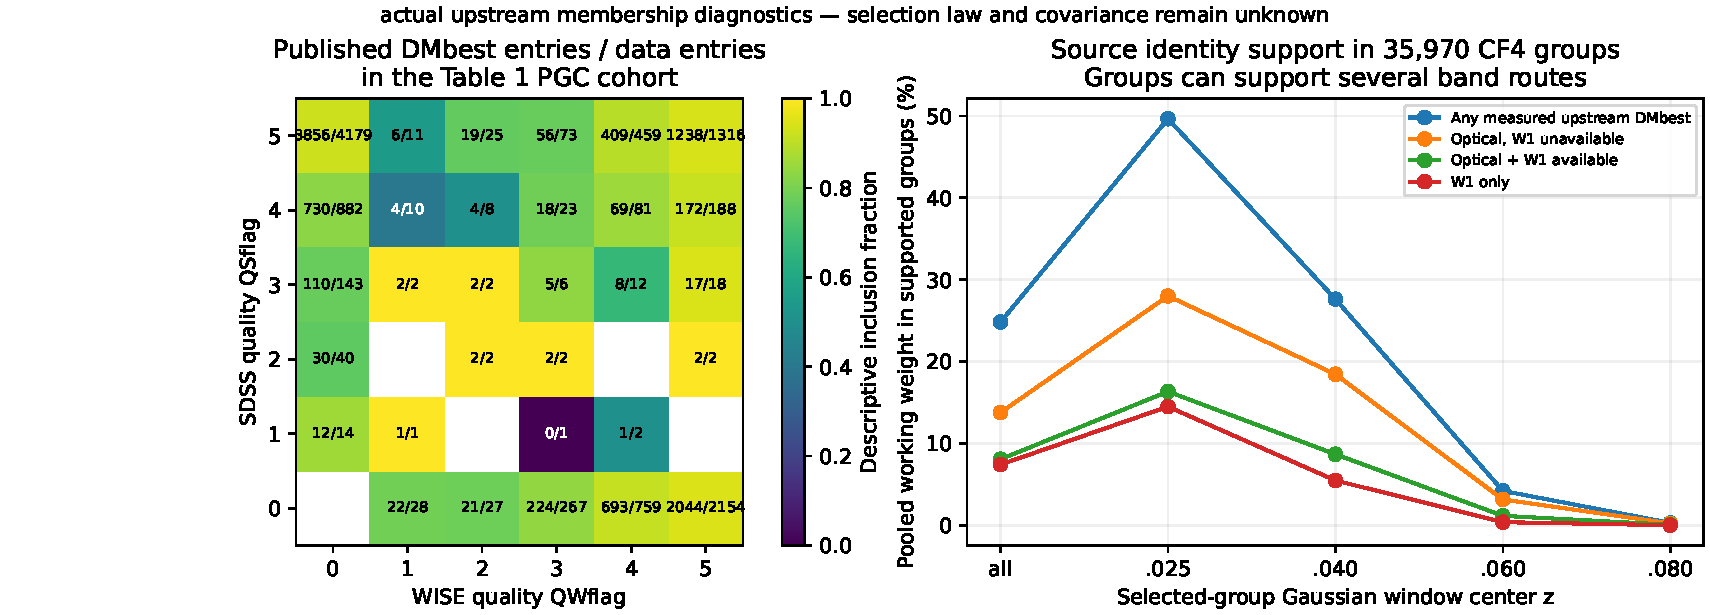
\includegraphics[width=\linewidth,height=.71\textheight,keepaspectratio]{figures/f024_external.pdf}
\caption{Upstream targeting and quality marks in released distance tables. Availability of a best modulus varies with the retained source marks. The table comparisons describe released membership; they do not make quality-dependent missingness ignorable.}
\label{fig:f024}
\end{figure}
\clearpage
\begin{figure}[p]
\centering
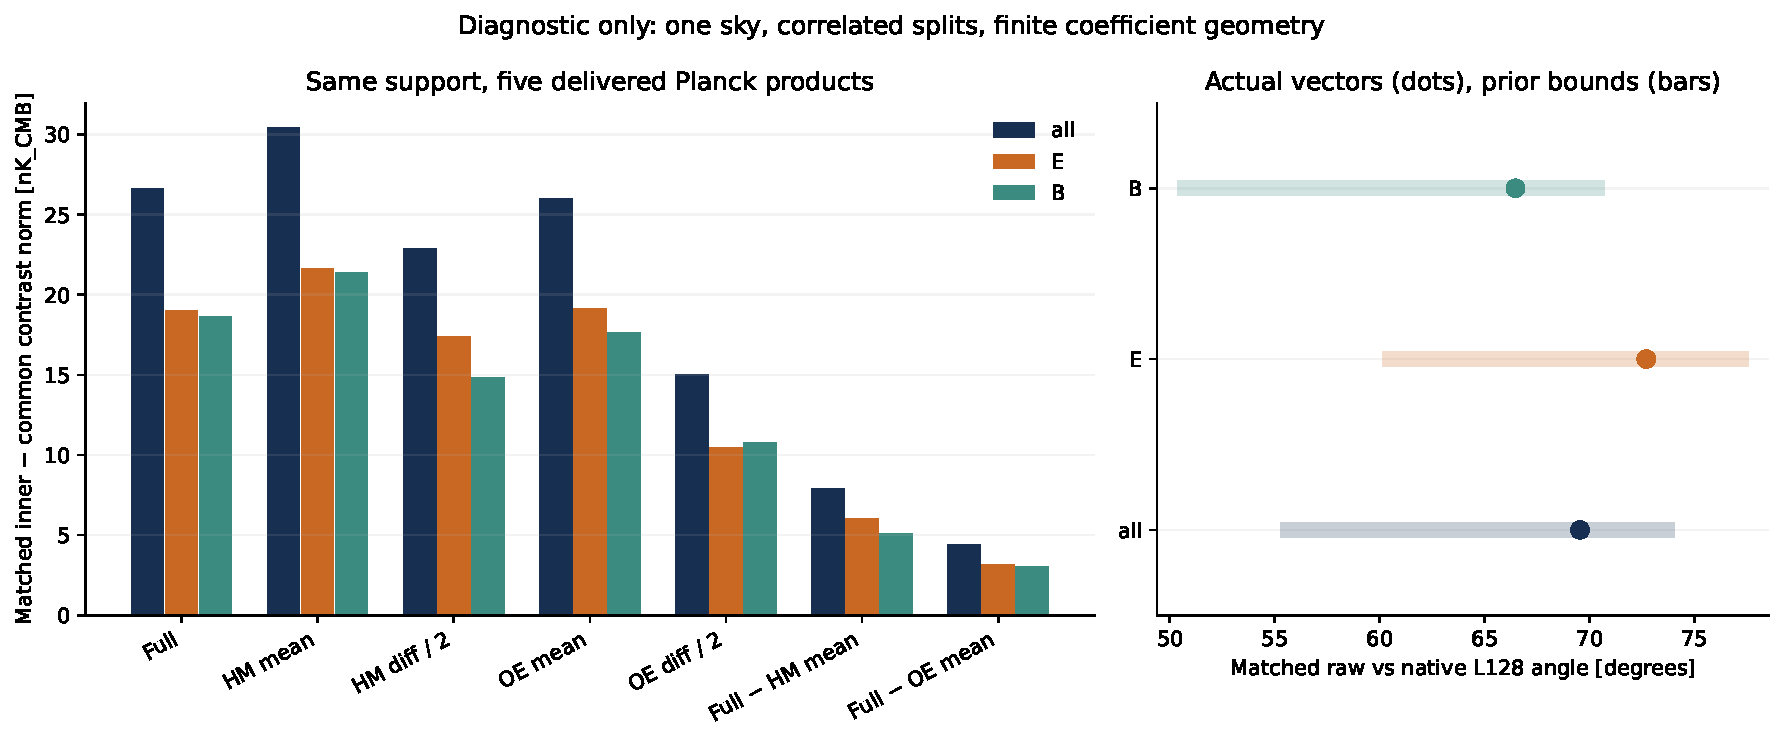
\includegraphics[width=\linewidth,height=.71\textheight,keepaspectratio]{figures/f025.pdf}
\caption{Matched processing contrasts on the same selected sky for five delivered Planck products. Actual vector differences are compared with the corresponding finite geometric bounds. Component norms cannot be added as though the components were aligned, and splits remain correlated views of one sky.}
\label{fig:f025}
\end{figure}
\clearpage
\begin{figure}[p]
\centering
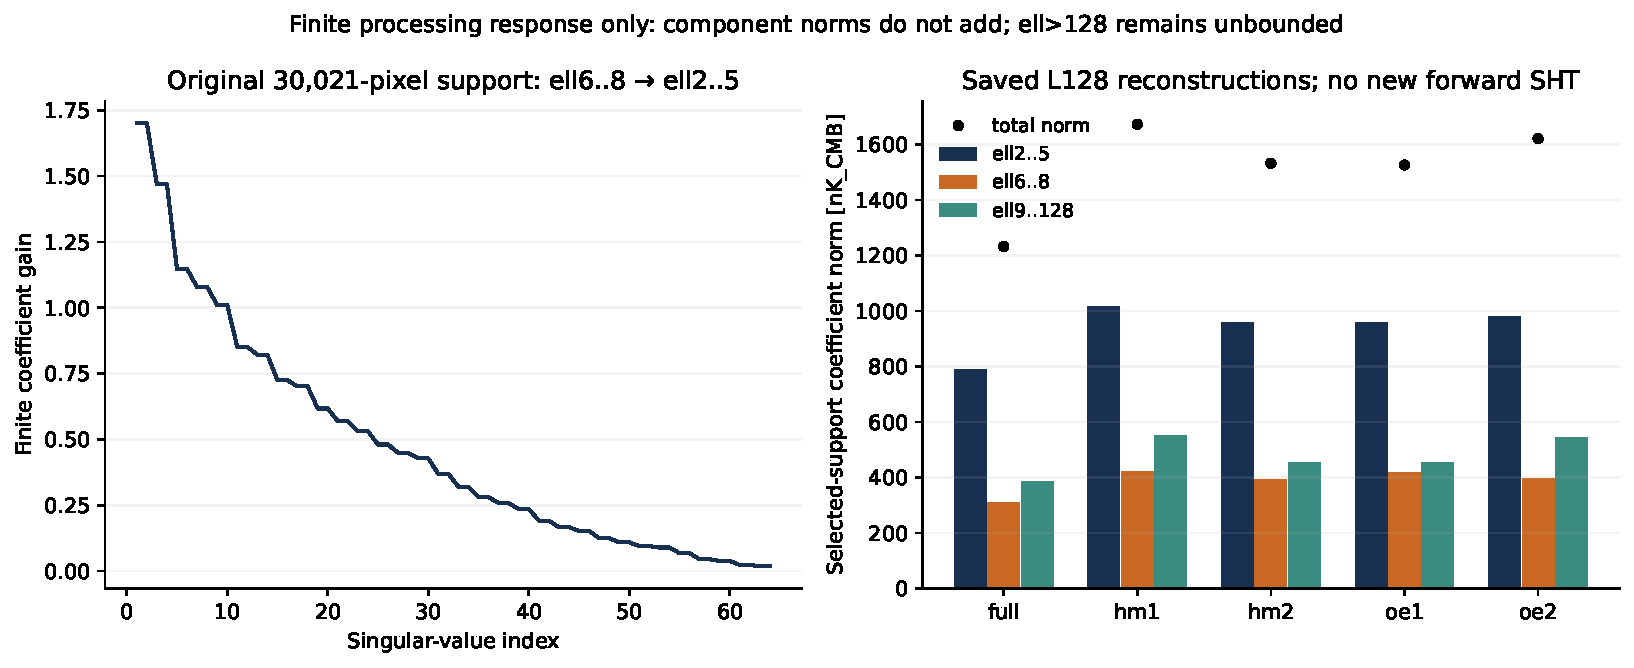
\includegraphics[width=\linewidth,height=.71\textheight,keepaspectratio]{figures/f026.pdf}
\caption{Finite higher-to-lower multipole response on the original selected polarization support. The leakage gains and retained reconstructions quantify an observation operator. Unknown higher-mode amplitudes and the omitted tail are not set to zero; no cosmic B-mode bound follows from operator gain alone.}
\label{fig:f026}
\end{figure}
\clearpage
\begin{figure}[p]
\centering
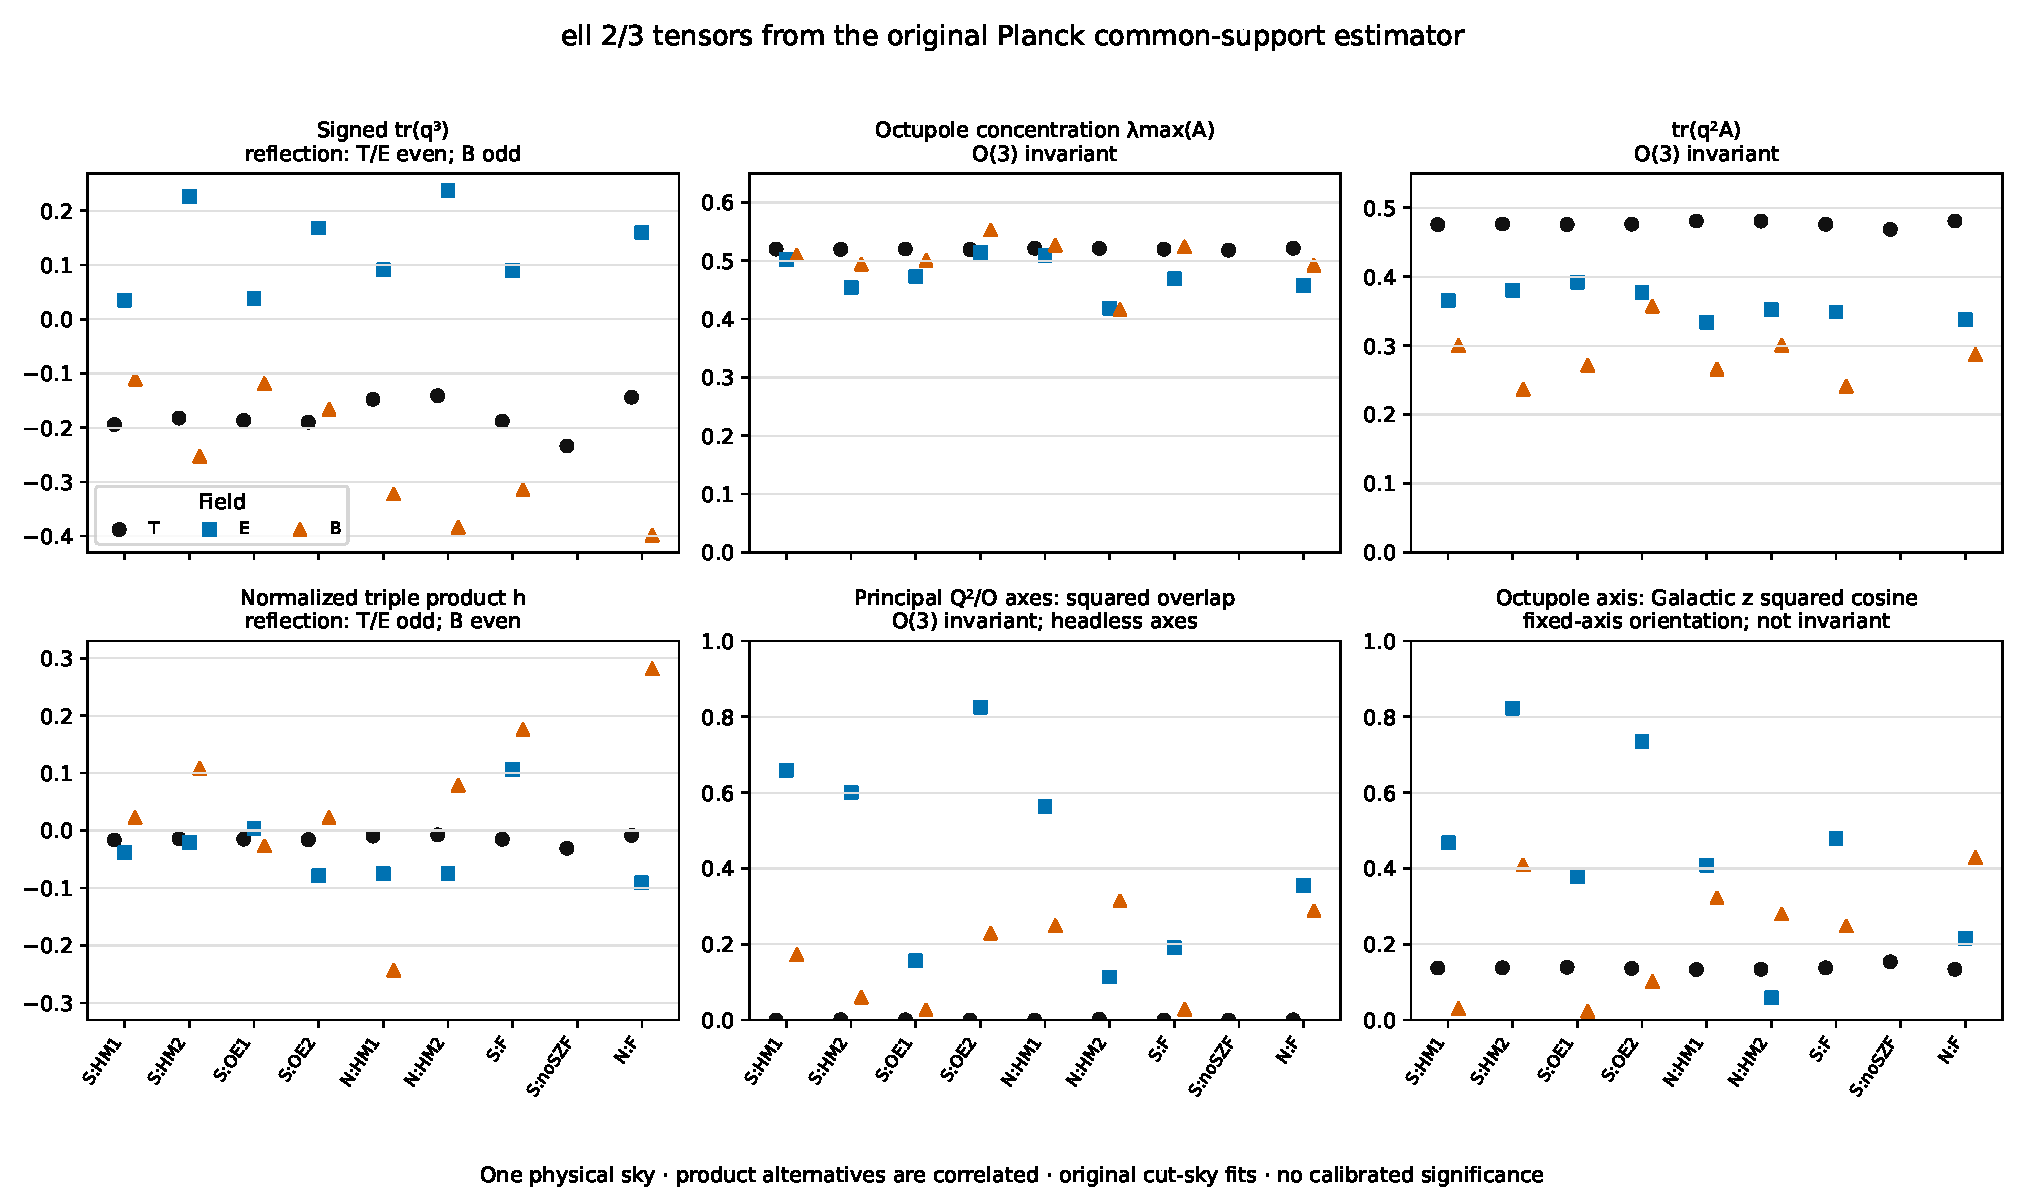
\includegraphics[width=\linewidth,height=.71\textheight,keepaspectratio]{figures/f027_external.pdf}
\caption{Signed shape and orientation descriptors of temperature and polarization multipoles from the original common-support estimator. Polar and axial parity are distinguished. These incomplete descriptors and same-sky product ranges do not provide a calibrated null probability or complete orbit classification.}
\label{fig:f027}
\end{figure}
\clearpage
\begin{figure}[p]
\centering
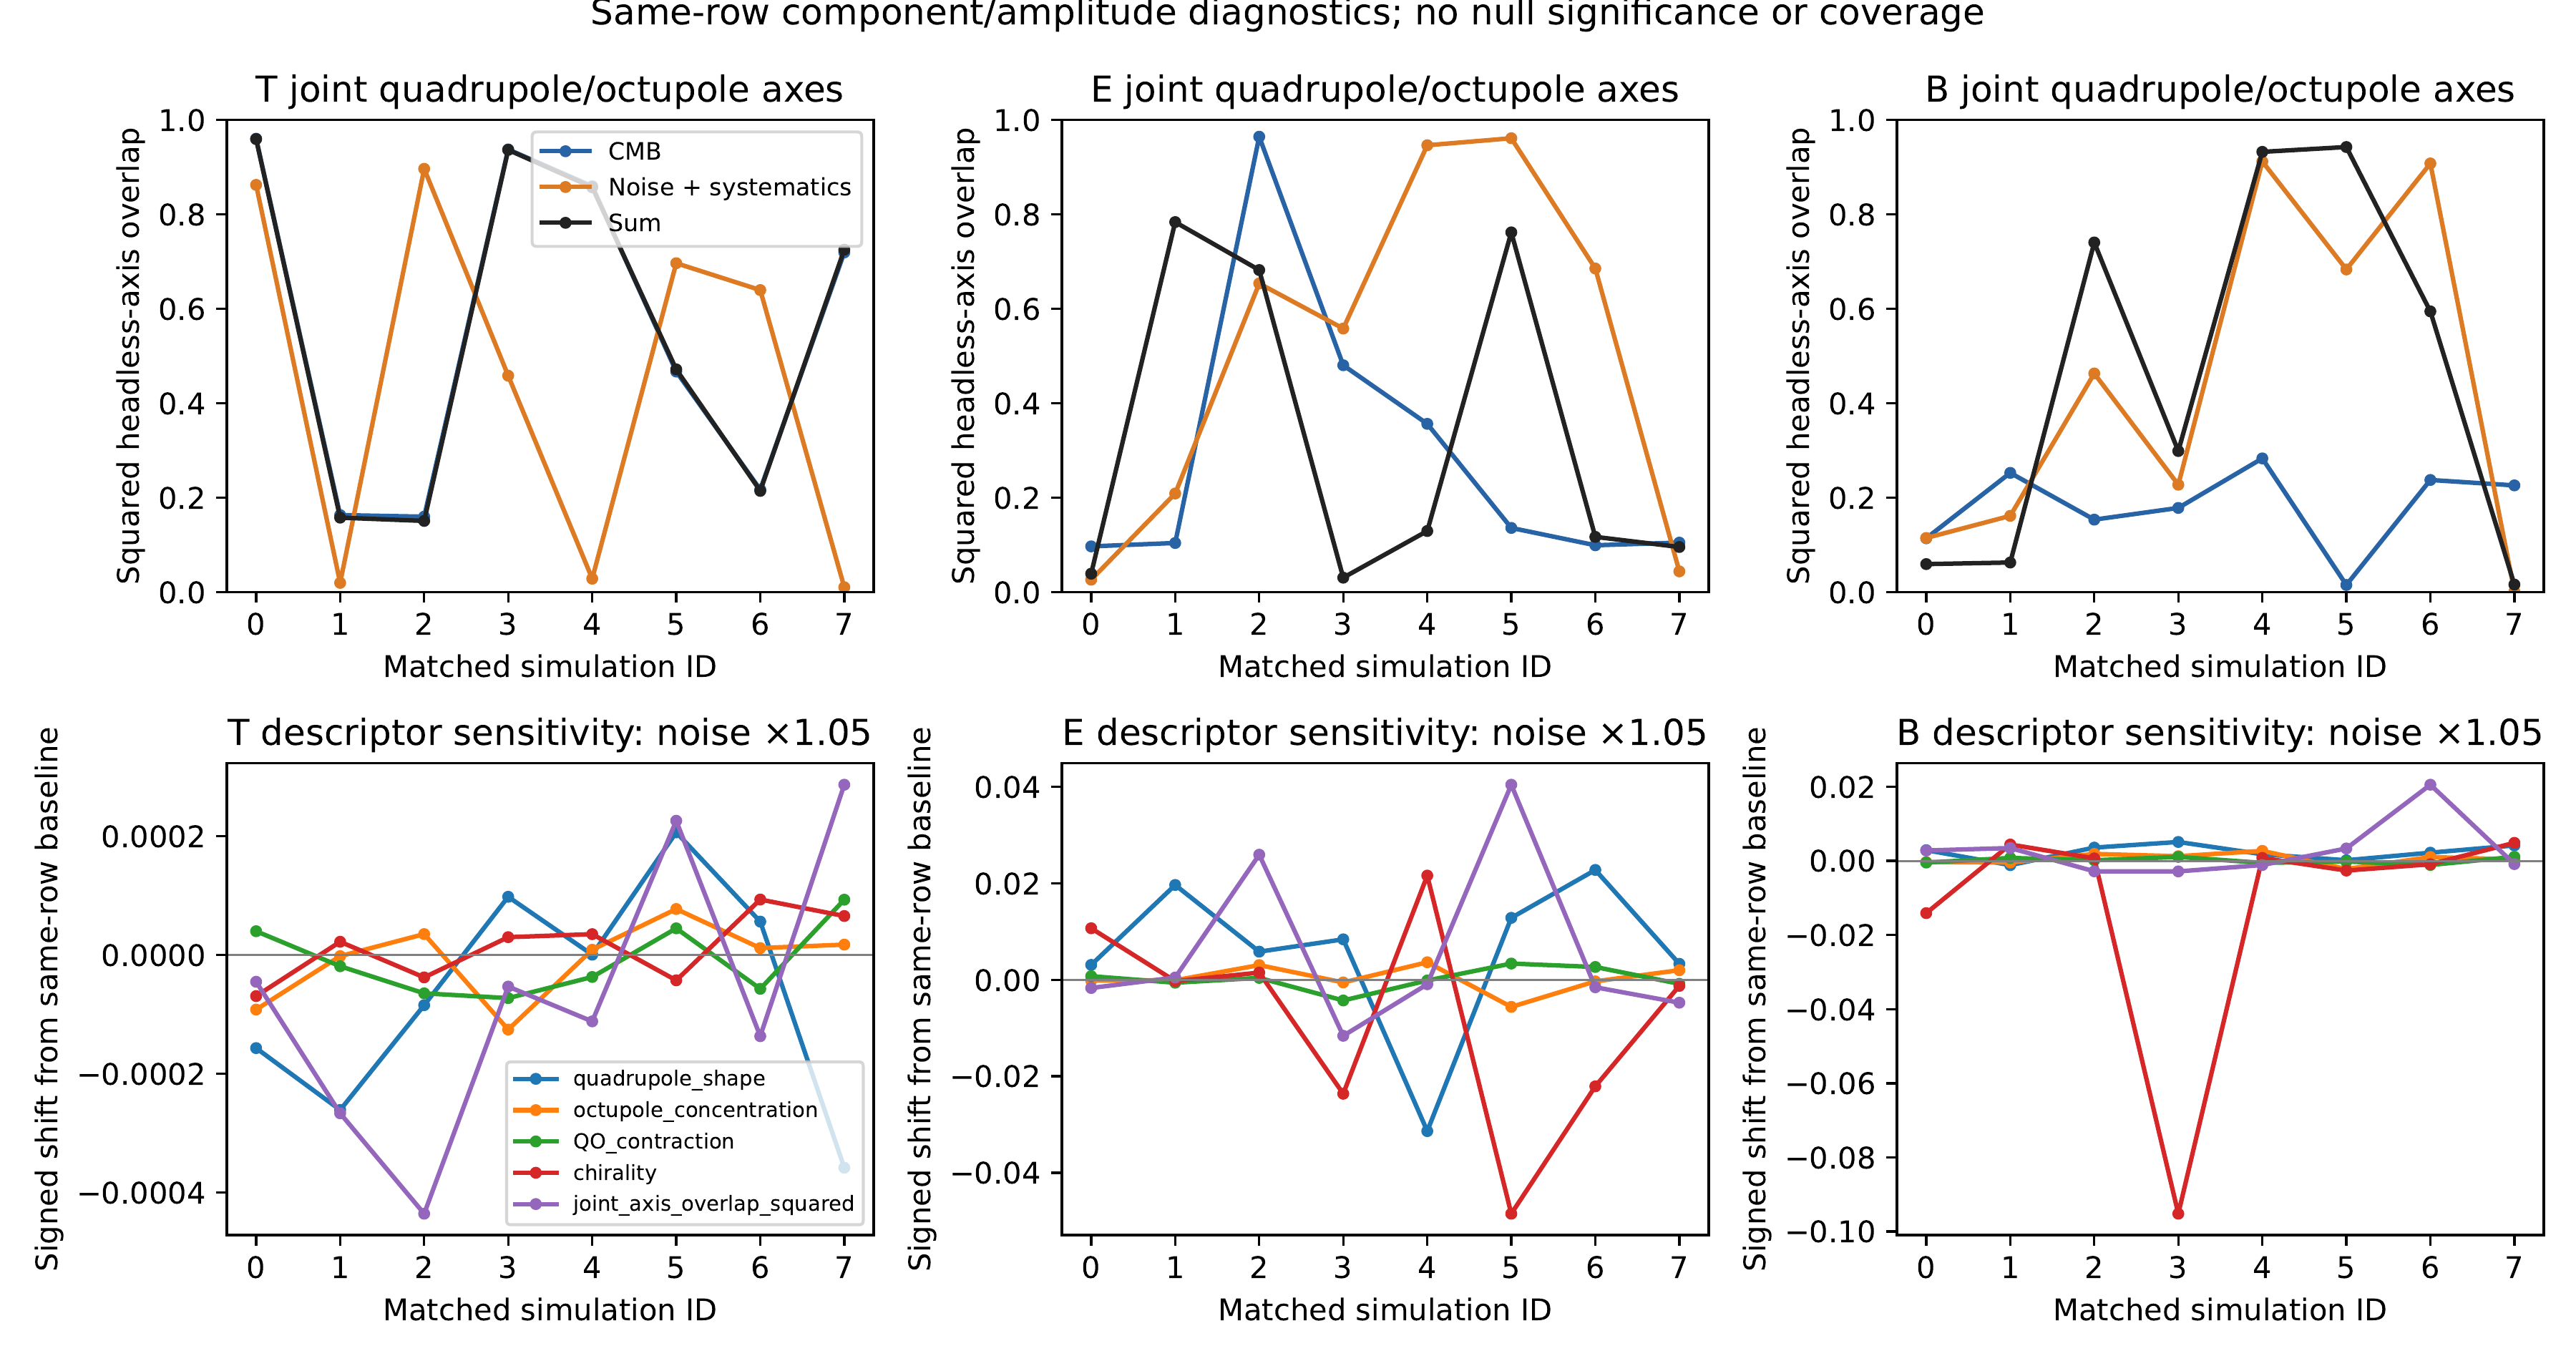
\includegraphics[width=\linewidth,height=.71\textheight,keepaspectratio]{figures/f028_external.png}
\caption{Tensor-descriptor sensitivity in eight matched signal/noise pairs. Each row retains its common source realization and processing. The small pilot and its noise-amplitude perturbation are finite response diagnostics, not an independently calibrated cosmological ensemble.}
\label{fig:f028}
\end{figure}
\clearpage
\begin{figure}[p]
\centering
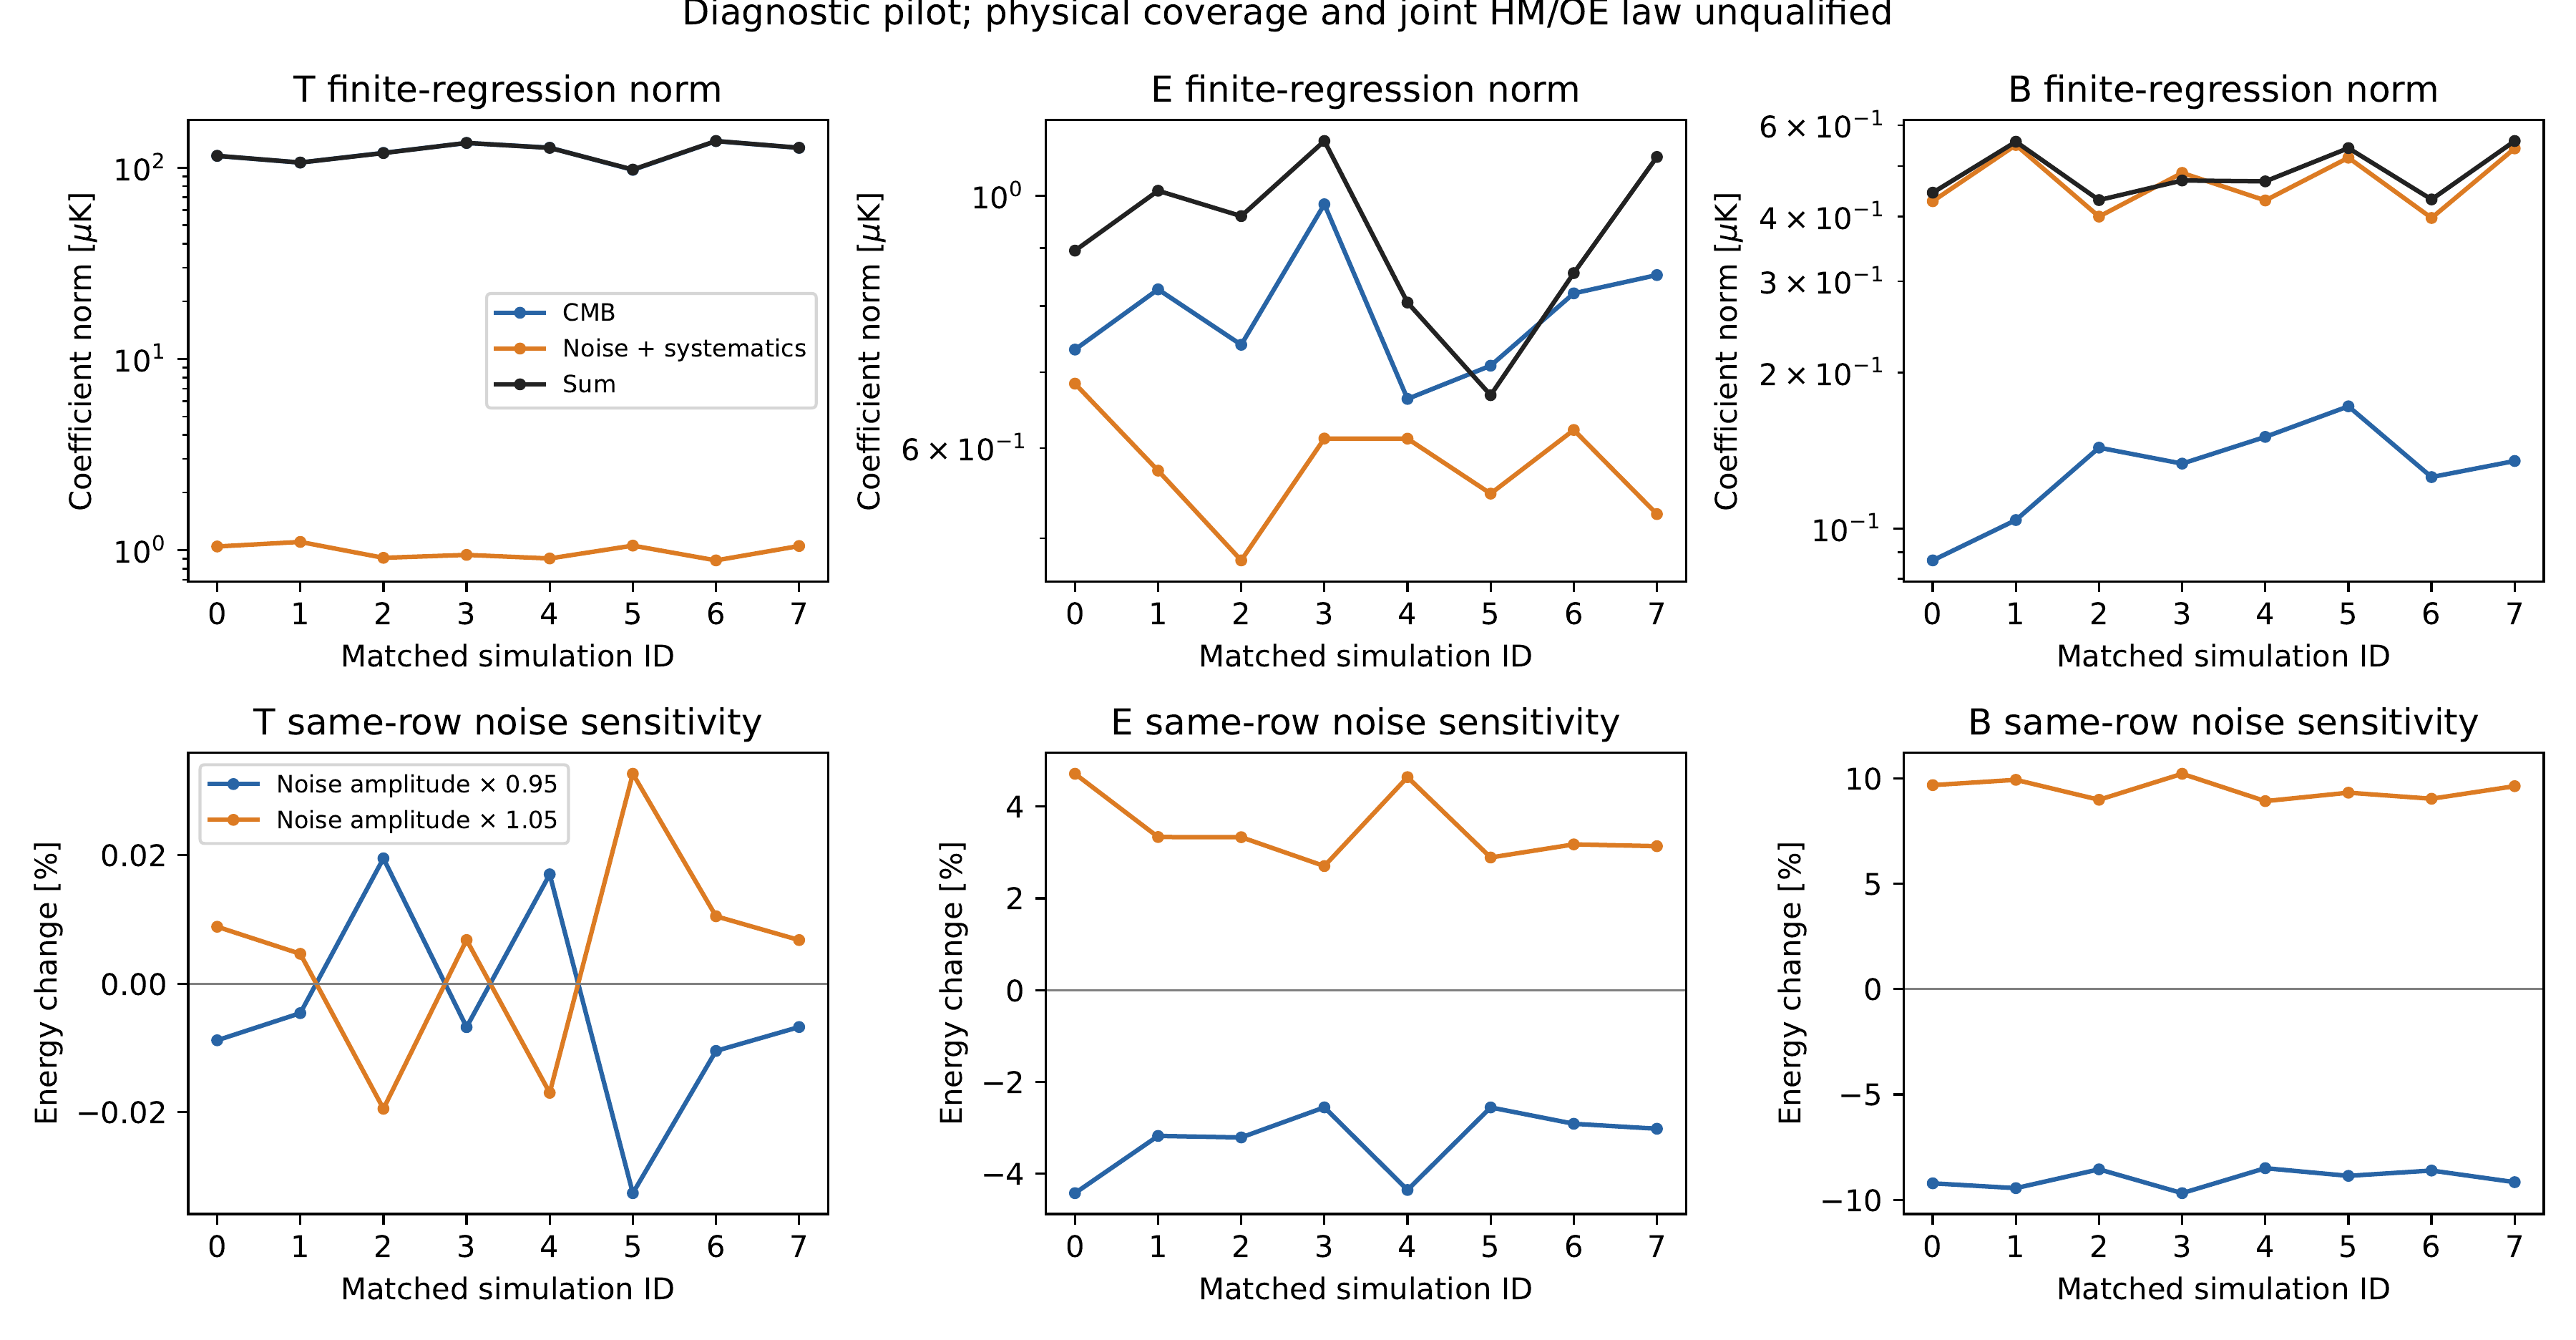
\includegraphics[width=\linewidth,height=.71\textheight,keepaspectratio]{figures/f029_external.png}
\caption{Joint coefficient diagnostics for eight retained Planck signal/noise pairs processed with the same original child-average operator. The centred covariance in the larger joint coordinate space is singular and is not inverted. Physical coverage and the joint half-mission/odd-even source law remain unqualified.}
\label{fig:f029}
\end{figure}
\clearpage
\begin{figure}[p]
\centering
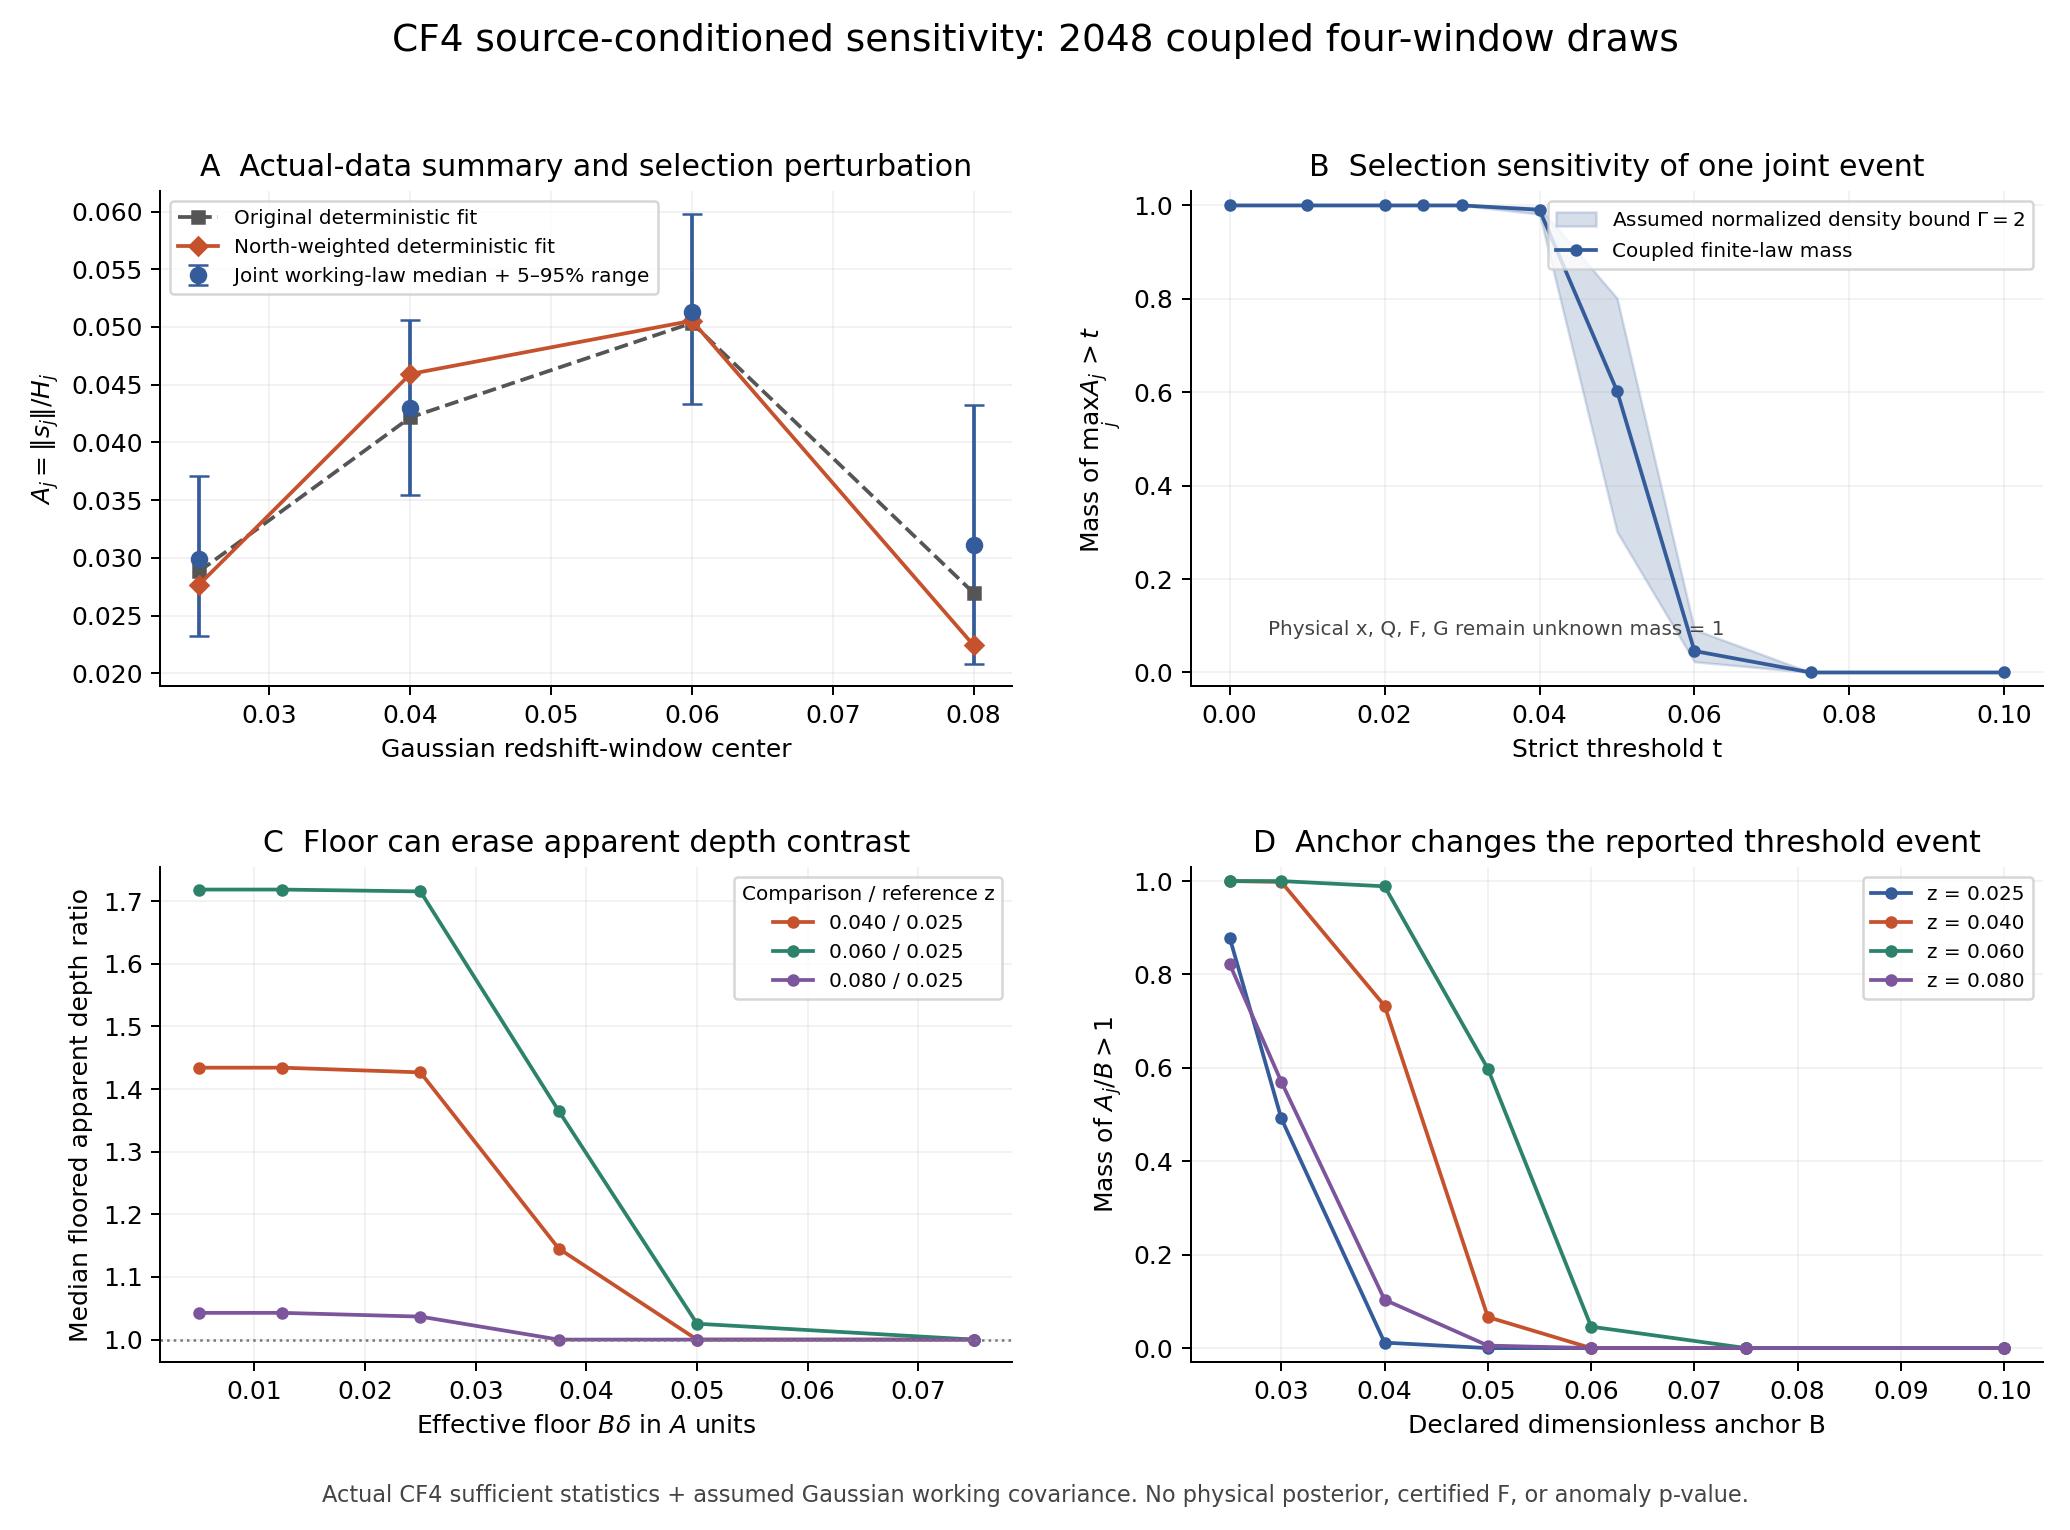
\includegraphics[width=\linewidth,height=.71\textheight,keepaspectratio]{figures/f030.png}
\caption{Functional sensitivity under one coupled finite measure from the four-window Cosmicflows fit. The plots retain common draw identity, declared anchors, positive floors, and strict ties. These are conditional changes in functionals and occupancies, not physical posterior probabilities.}
\label{fig:f030}
\end{figure}
\clearpage
\begin{figure}[p]
\centering
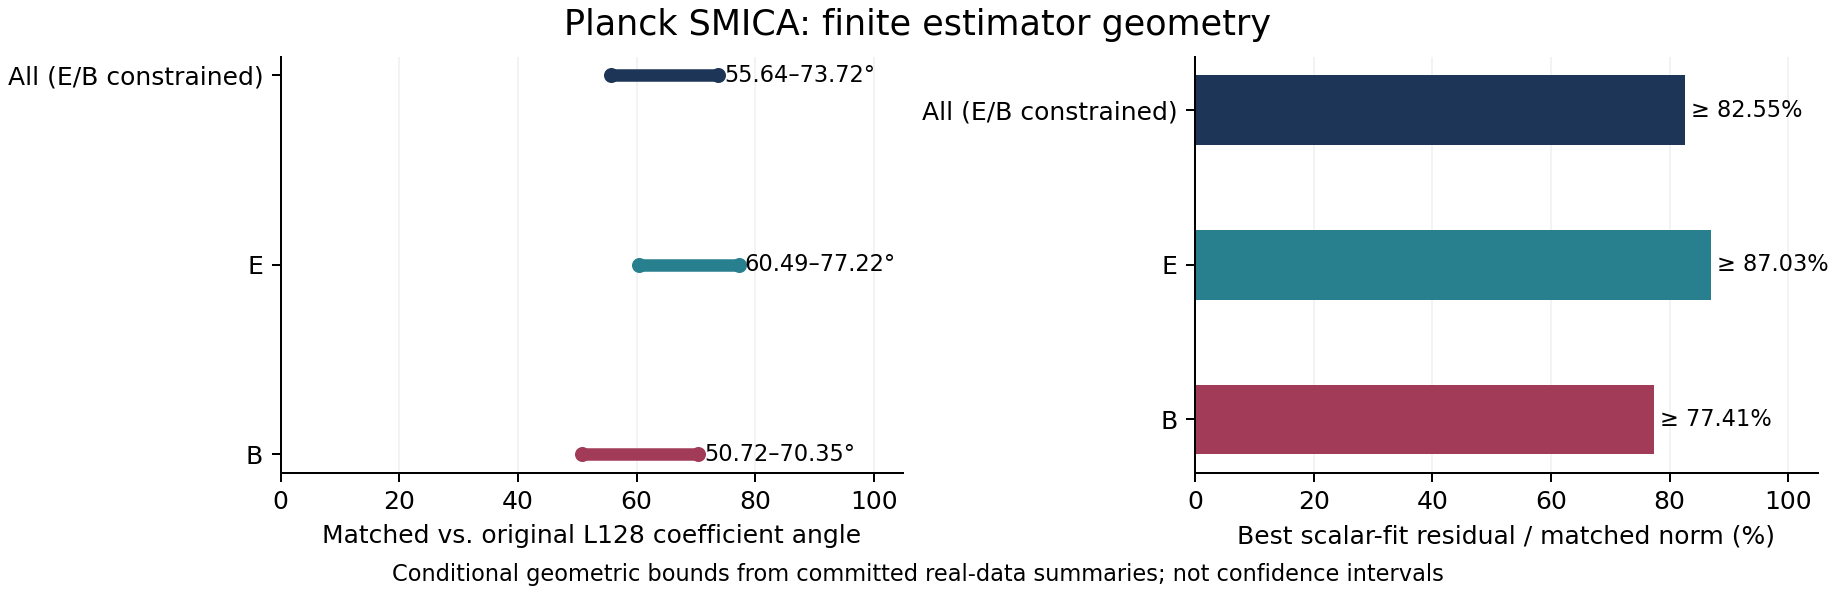
\includegraphics[width=\linewidth,height=.71\textheight,keepaspectratio]{figures/f031.png}
\caption{Finite Planck anchor geometry from the retained processed components. Orthogonal E/B blocks sharpen particular norm bounds, while missing cross orientation limits others. The anchors are computational summaries and do not certify a physical anisotropy ceiling.}
\label{fig:f031}
\end{figure}
\clearpage
\begin{figure}[p]
\centering
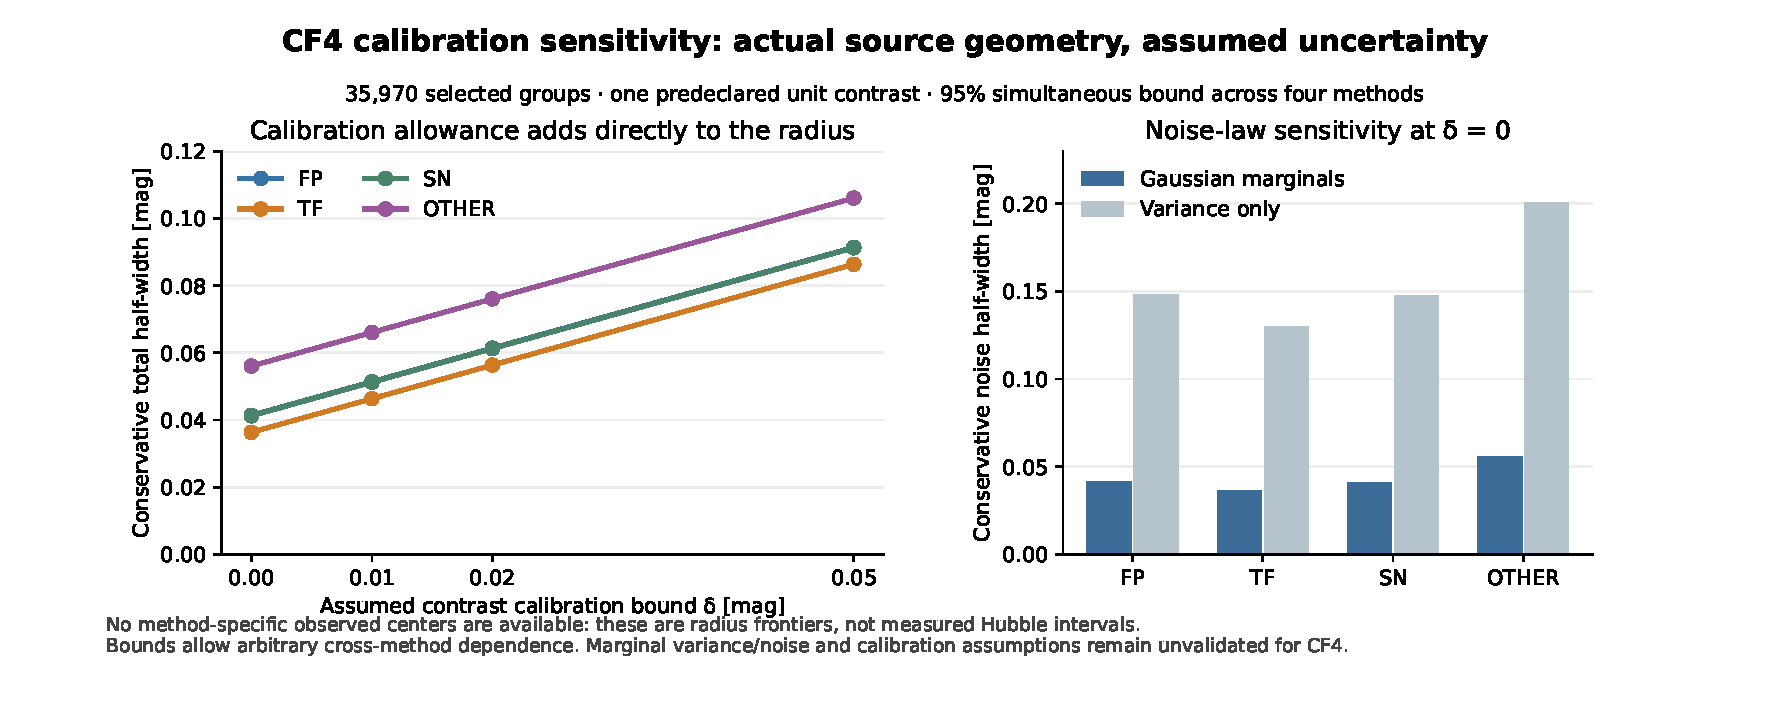
\includegraphics[width=\linewidth,height=.71\textheight,keepaspectratio]{figures/f032_external.pdf}
\caption{Calibration-radius sensitivity on the actual Cosmicflows source geometry. The selected contrast and simultaneous working reference are fixed; the horizontal radius is assumed. A radius-only frontier does not supply observed calibration centres or an empirically measured systematic bound.}
\label{fig:f032}
\end{figure}
\clearpage
\begin{figure}[p]
\centering
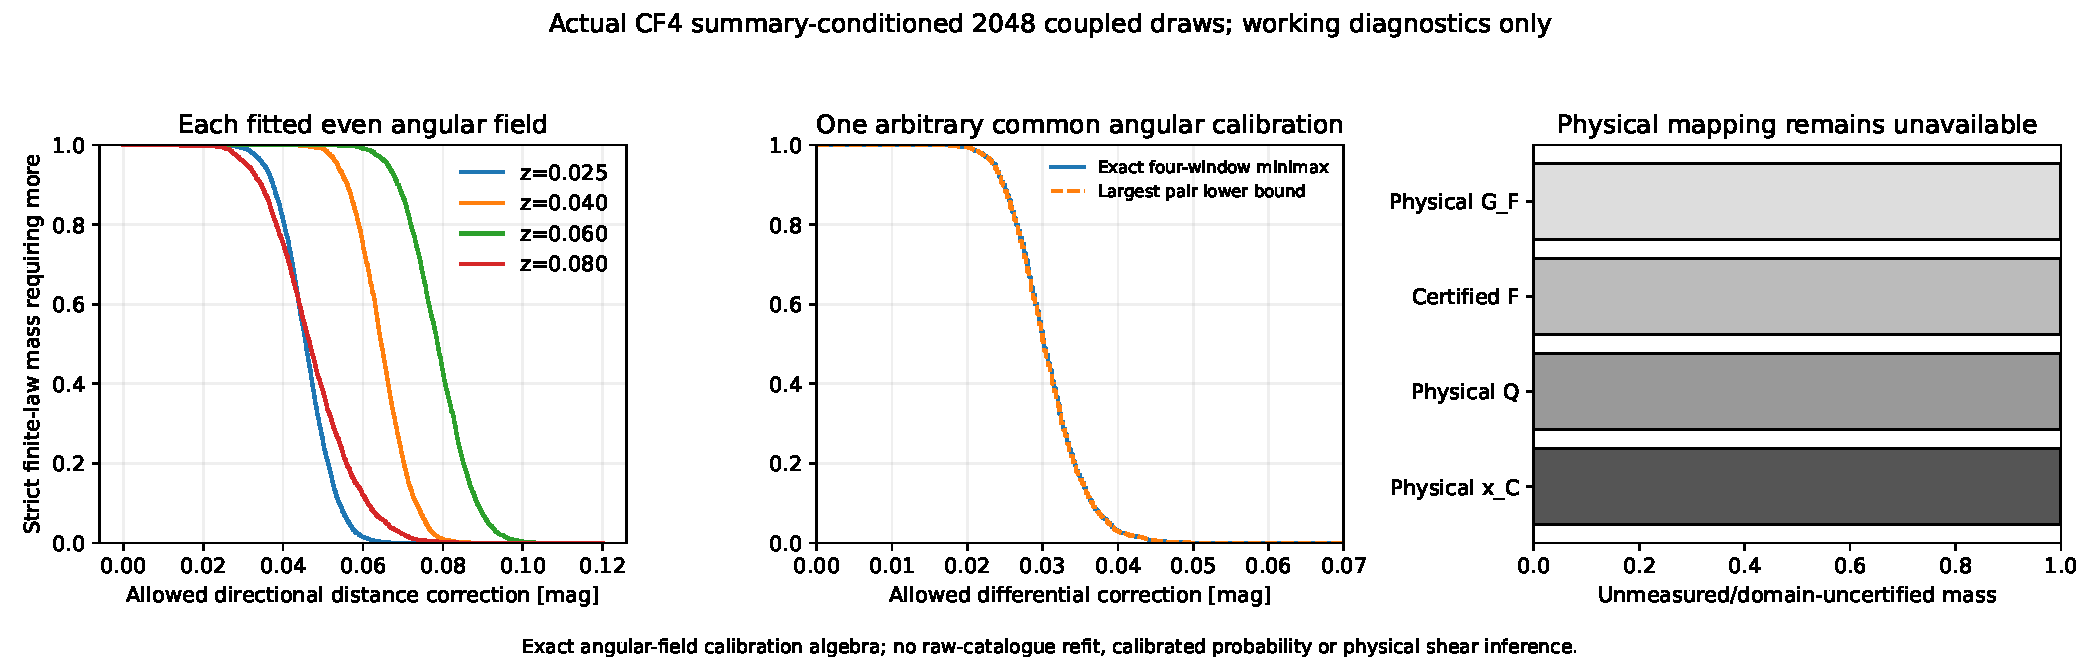
\includegraphics[width=\linewidth,height=.71\textheight,keepaspectratio]{figures/f033_external.pdf}
\caption{Calibration obstruction for the coupled group-fit finite measure. The panels distinguish independently fitted angular fields from one shared angular calibration. Their exceedances refer to the retained working measure, with physical completion and source covariance still unqualified.}
\label{fig:f033}
\end{figure}
\clearpage
\begin{figure}[p]
\centering
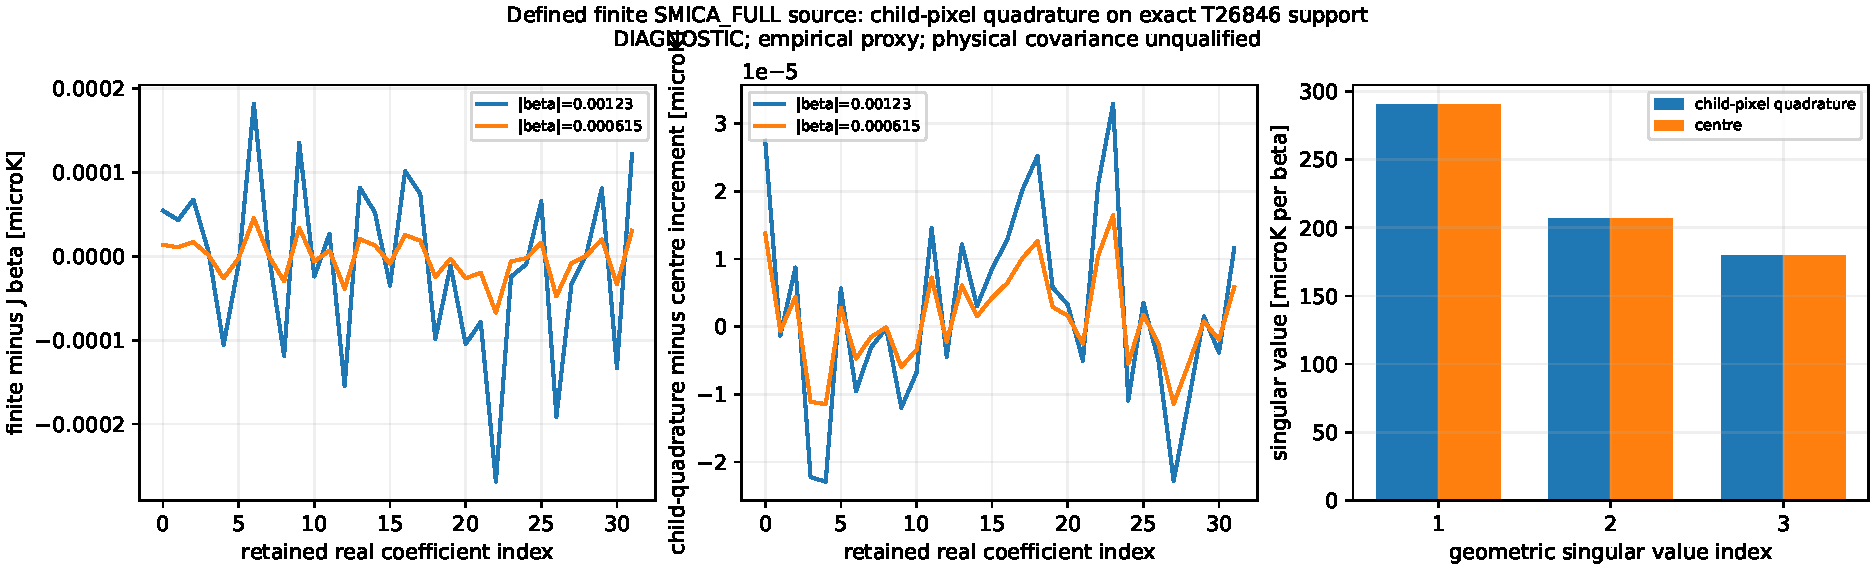
\includegraphics[width=\linewidth,height=.71\textheight,keepaspectratio]{figures/f034_external.pdf}
\caption{Finite delivered-map observer-response calculation at child-pixel resolution, compared with a pixel-centre approximation. The mask and source field are fixed. Differences and finite-minus-linear residuals characterize that processing response, not a cosmological transfer history or calibrated spatial covariance.}
\label{fig:f034}
\end{figure}
\clearpage
\begin{figure}[p]
\centering
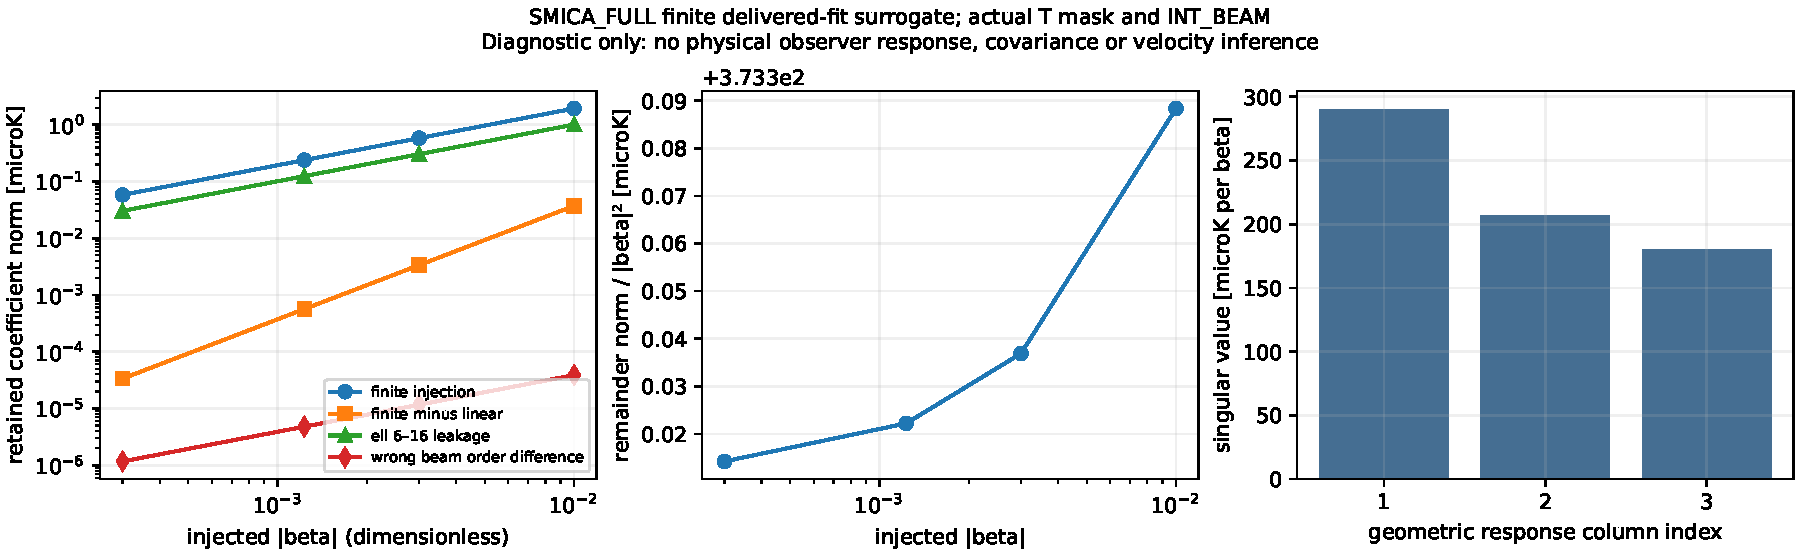
\includegraphics[width=\linewidth,height=.71\textheight,keepaspectratio]{figures/f035.pdf}
\caption{Finite observer-boost interventions and linear-response residuals for a declared delivered map. Higher-mode content and beam order alter the result. The curves test this finite response model; they do not establish a complete physical source history or null law.}
\label{fig:f035}
\end{figure}
\clearpage
\begin{figure}[p]
\centering
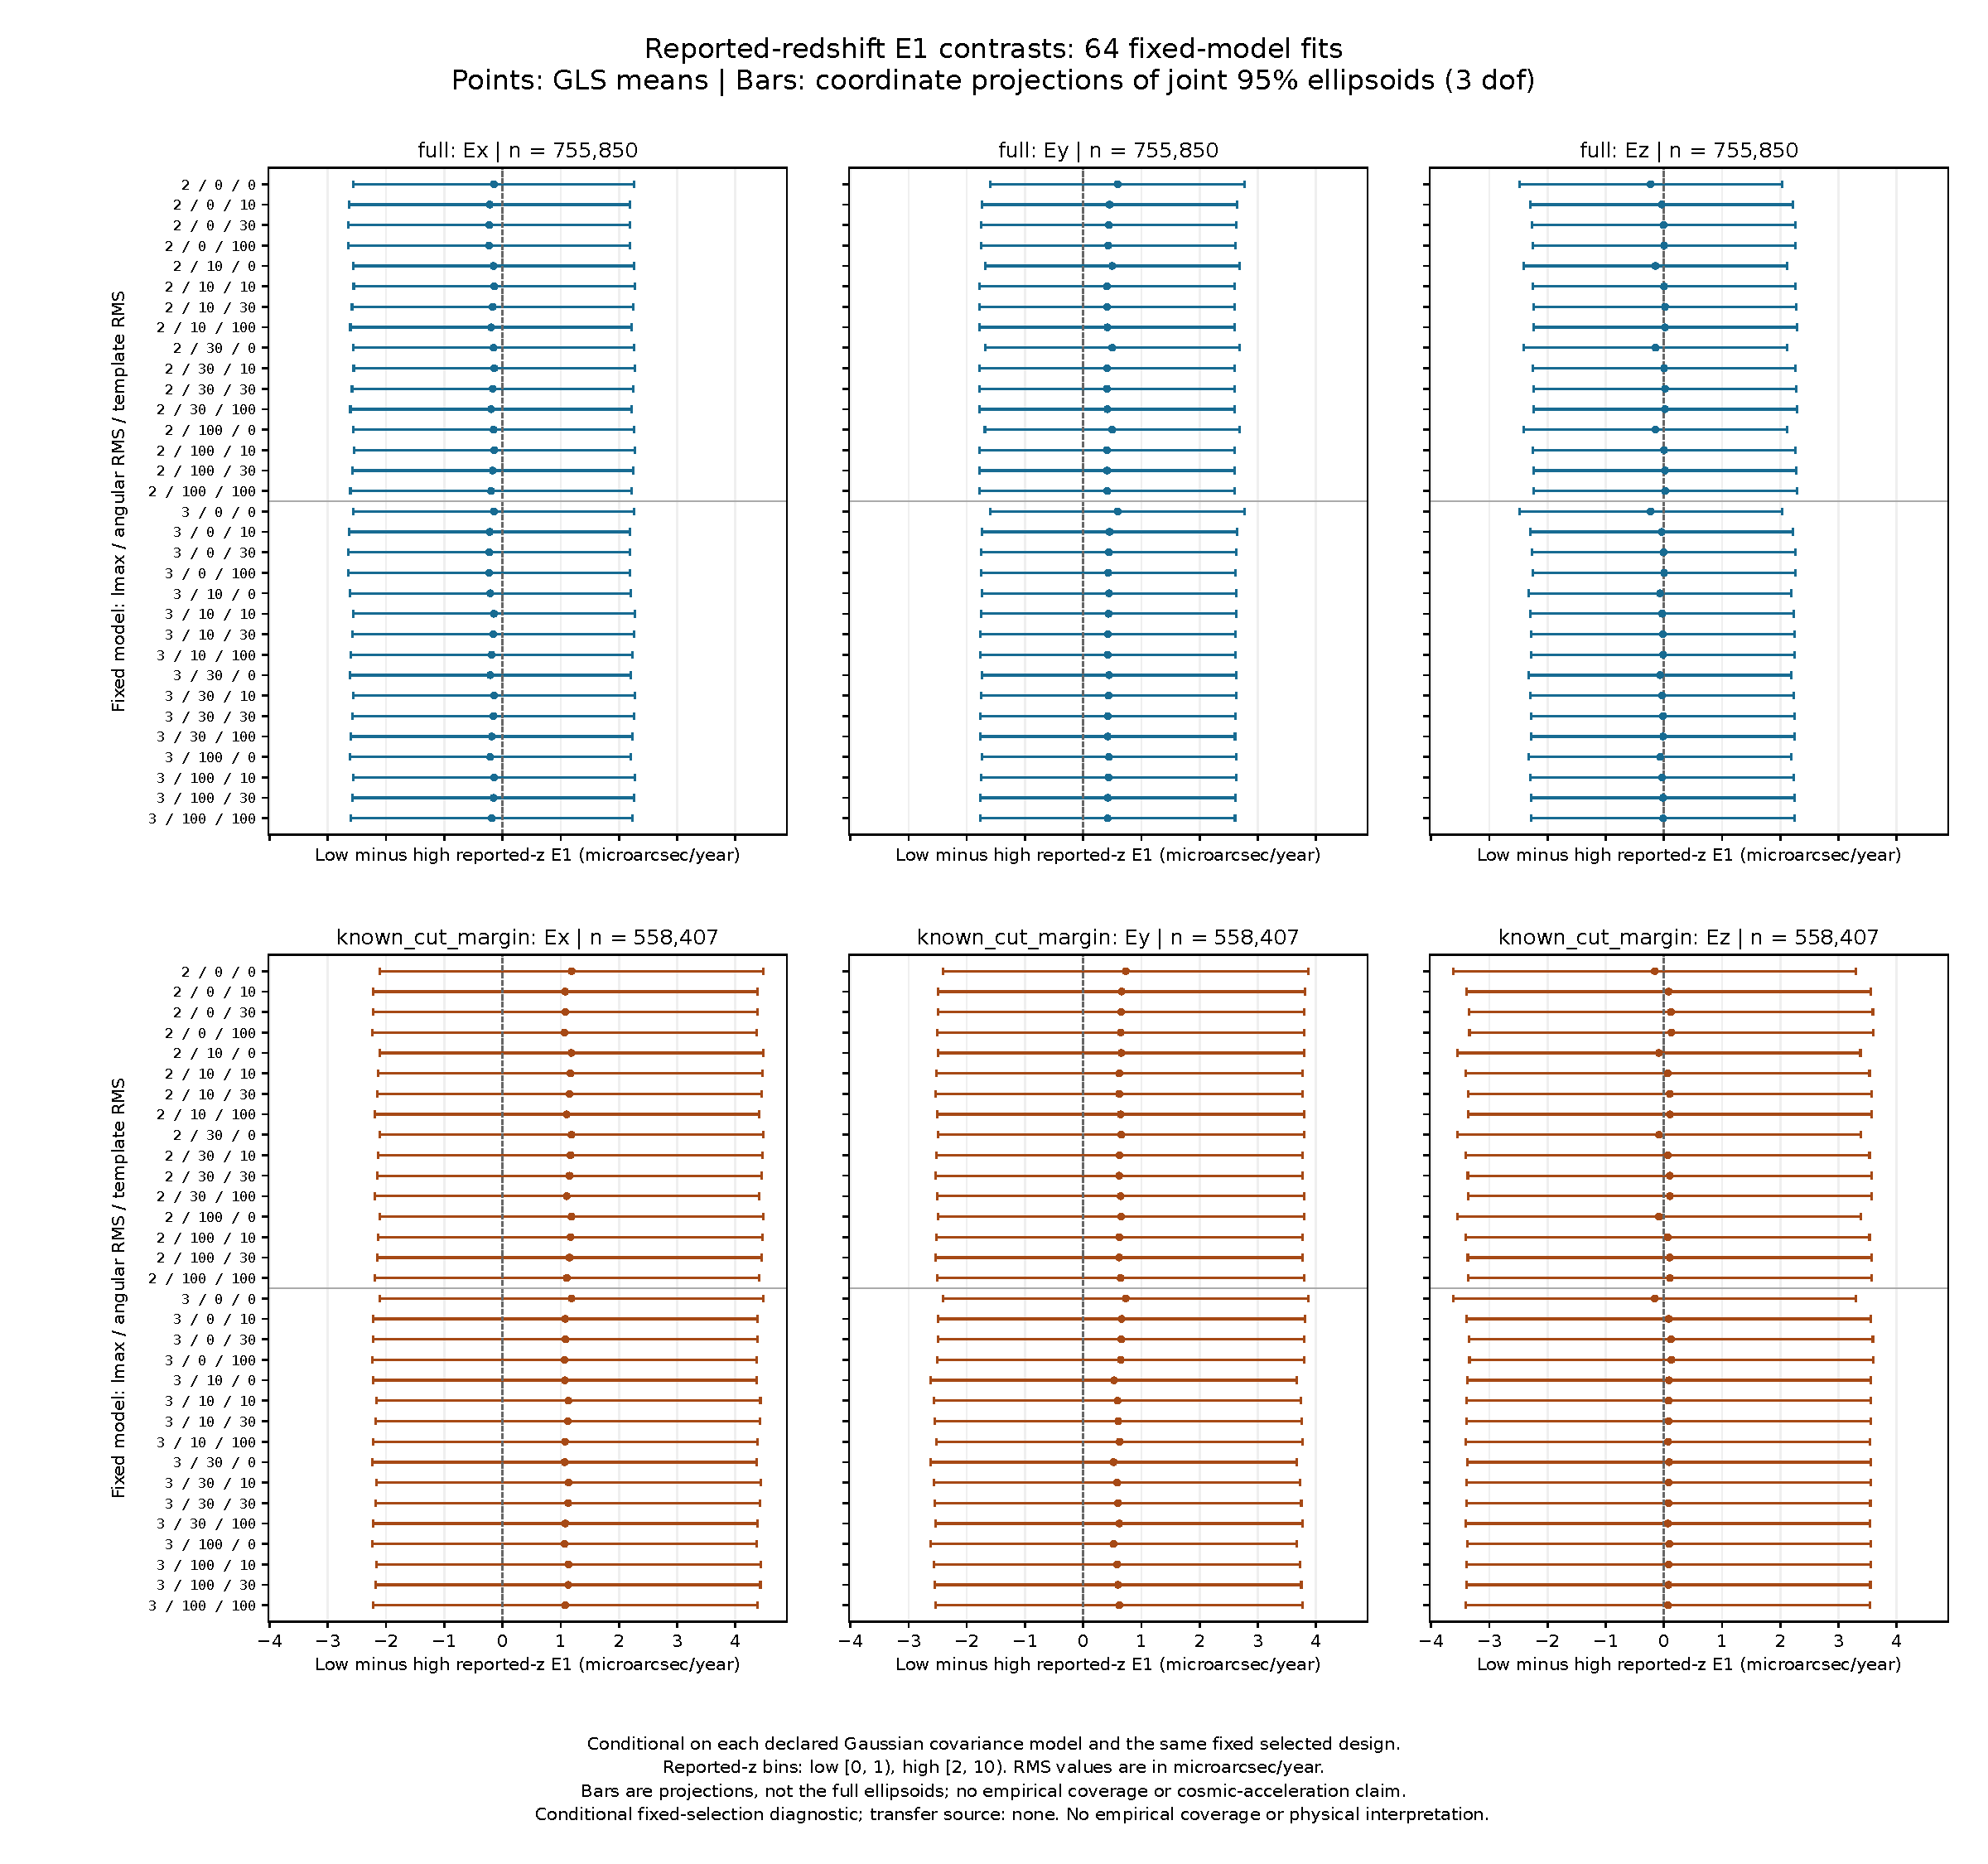
\includegraphics[width=\linewidth,height=.71\textheight,keepaspectratio]{figures/f036_external.pdf}
\caption{Low-minus-high reported-redshift astrometric contrast under the stated covariance scenarios. Shared bins and nuisance responses are retained. This is a conditional coordinate contrast; reported redshift, spatial covariance, and source-centroid response are not a calibrated physical depth experiment.}
\label{fig:f036}
\end{figure}
\clearpage
\begin{figure}[p]
\centering
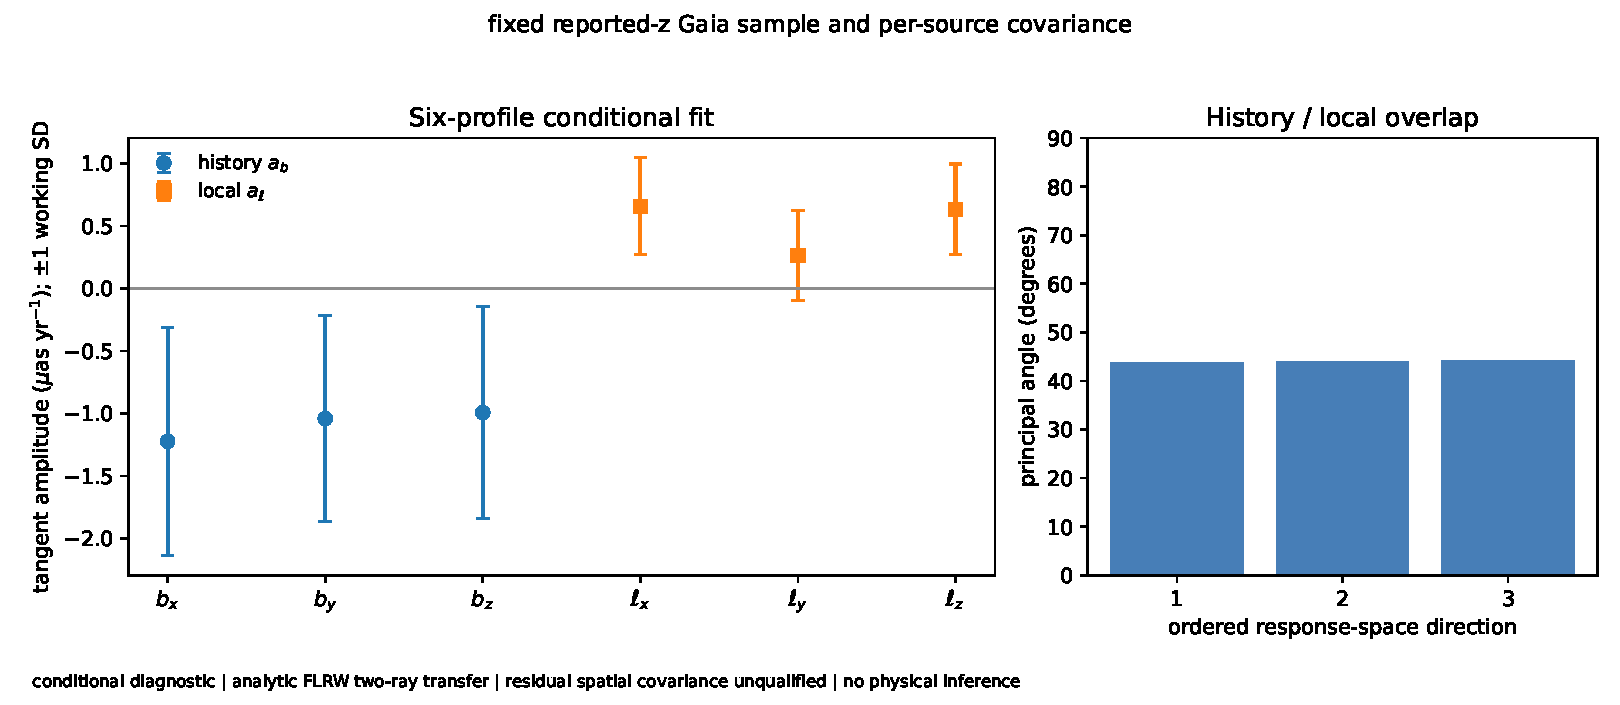
\includegraphics[width=\linewidth,height=.71\textheight,keepaspectratio]{figures/f037_external.pdf}
\caption{Profiled history and local-response coefficients and their principal-angle geometry in the retained astrometric design. Error bars use the stated working covariance. Full rank does not imply useful power within a small-response domain or establish a physical history.}
\label{fig:f037}
\end{figure}
\clearpage
\begin{figure}[p]
\centering
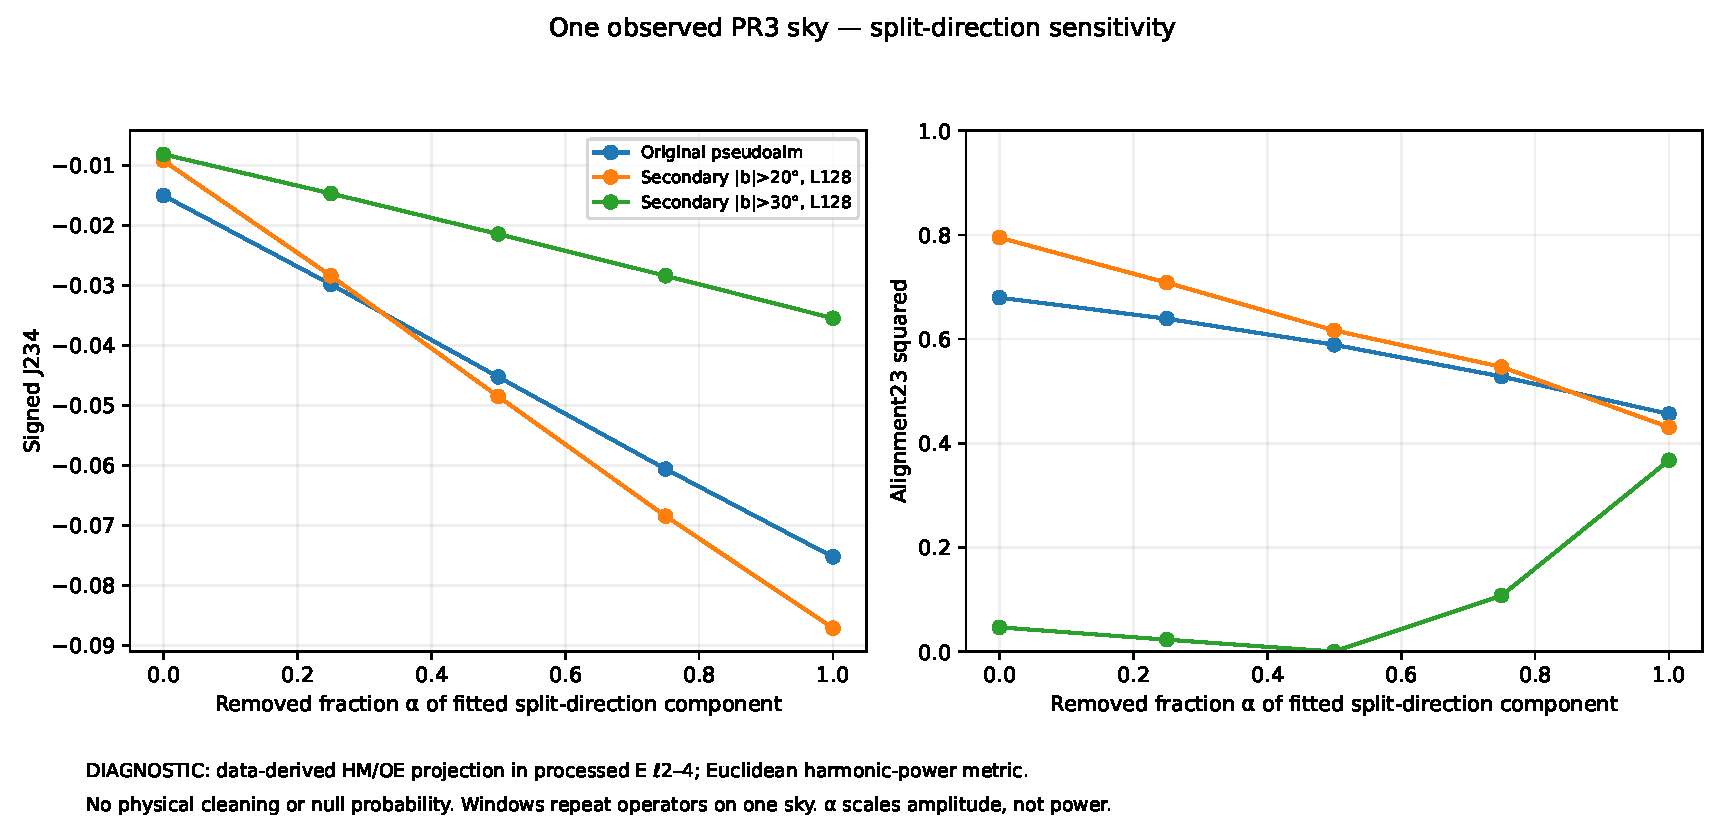
\includegraphics[width=\linewidth,height=.71\textheight,keepaspectratio]{figures/f039_external.pdf}
\caption{Sensitivity of processed E-pseudoalm morphology to split-direction projections on one Planck sky. The processing windows remain distinct. These projected comparisons do not remove an arbitrary common foreground or supply an exchangeable physical null.}
\label{fig:f039}
\end{figure}
\clearpage
\begin{figure}[p]
\centering
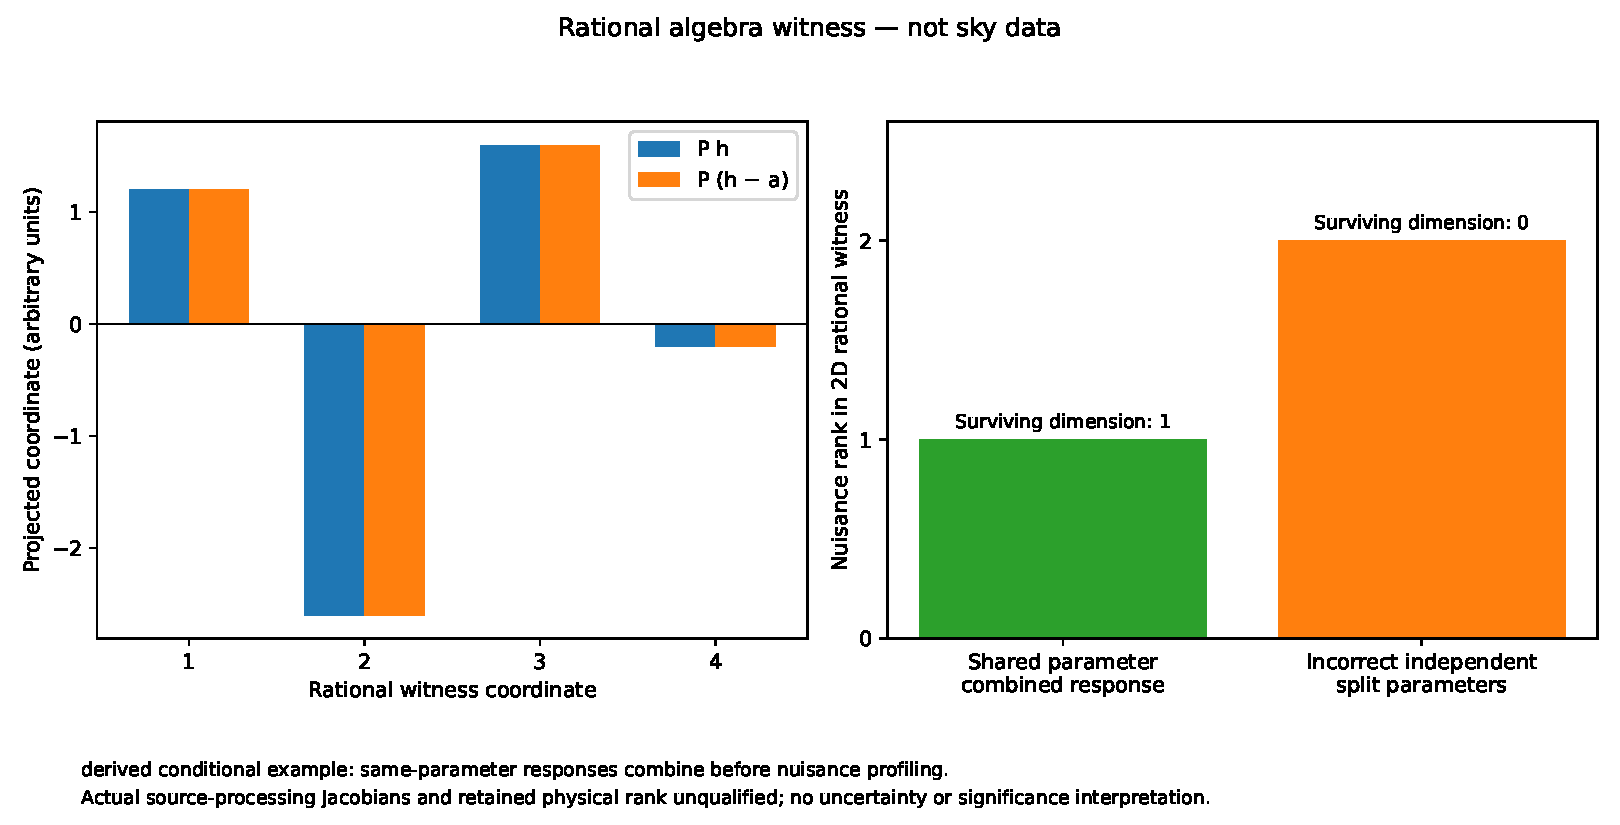
\includegraphics[width=\linewidth,height=.71\textheight,keepaspectratio]{figures/f040_external.pdf}
\caption{Exact rational nuisance-quotient counterexample. The displayed vectors and rank changes are constructed algebraic witnesses, not sky measurements. They show why a response can survive one nuisance span and disappear under a larger one.}
\label{fig:f040}
\end{figure}
\clearpage
\begin{figure}[p]
\centering
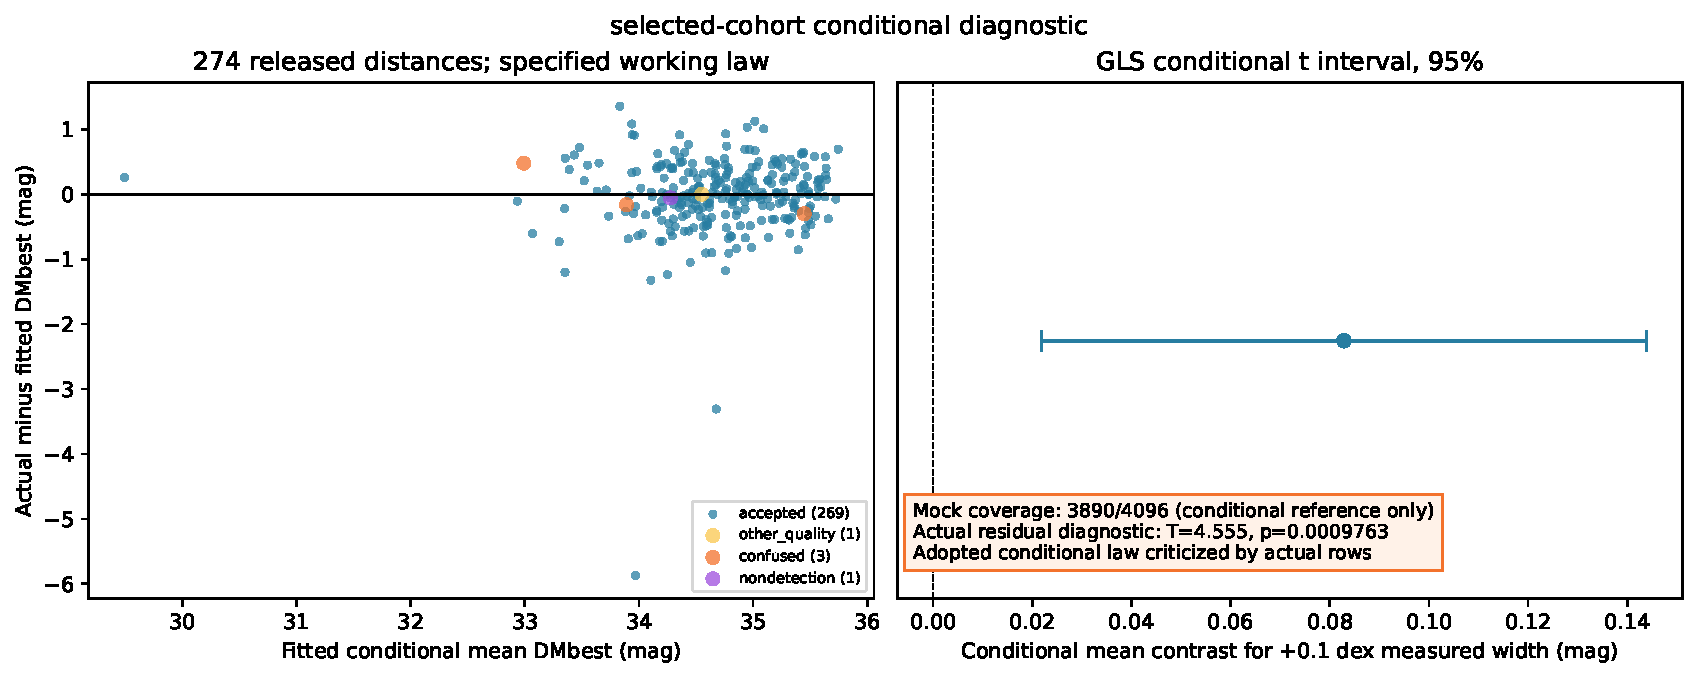
\includegraphics[width=\linewidth,height=.71\textheight,keepaspectratio]{figures/f041_external.pdf}
\caption{Actual-data residual criticism of the earlier selected-distance Gaussian model. The retained quality marks and simulation reference expose its failure on the observed cohort. Simulations generated under that model do not repair the failed actual-data check or validate later model variants.}
\label{fig:f041}
\end{figure}
\clearpage
\begin{figure}[p]
\centering
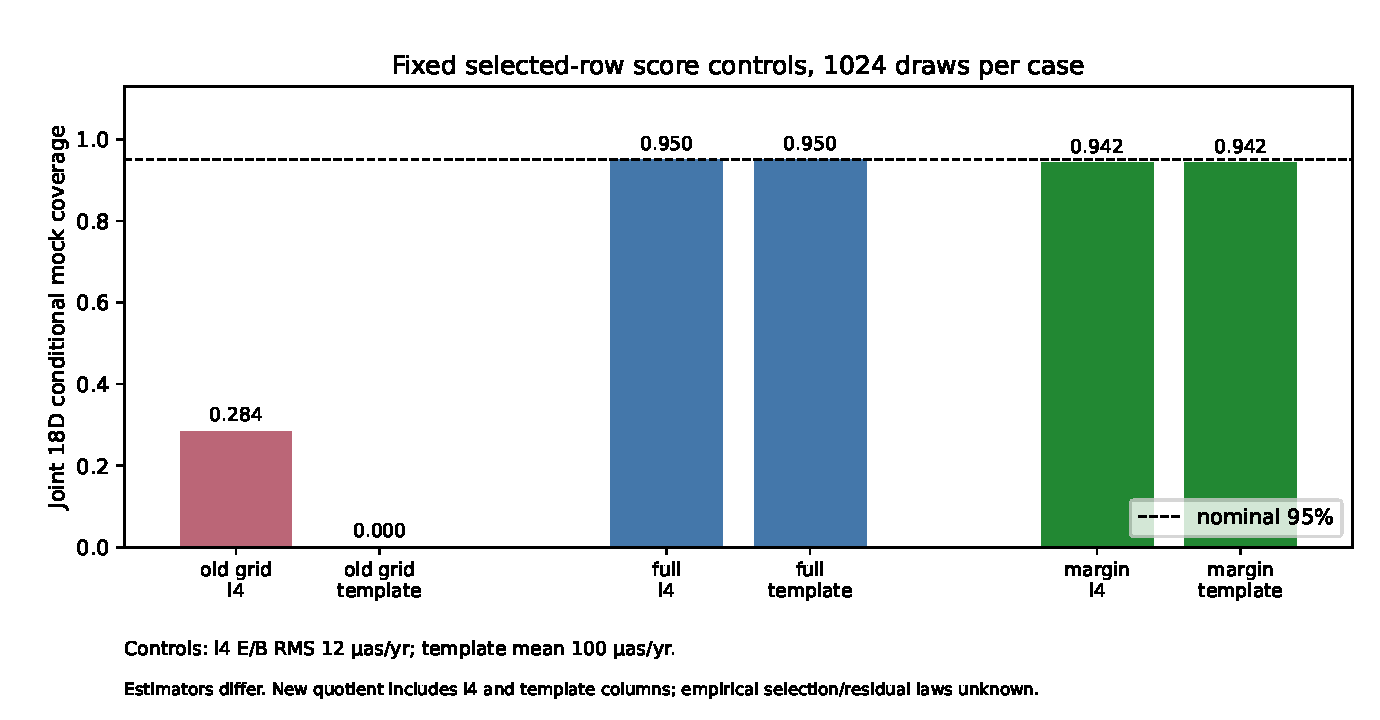
\includegraphics[width=\linewidth,height=.71\textheight,keepaspectratio]{figures/f042_external.pdf}
\caption{Synthetic astrometric coverage controls over 1024 realizations, comparing full and marginal fits under the stated generated laws. Omitted higher-order E4/B4 structure and a template-correlated mean substantially degrade nominal joint coverage. These are misspecification examples; they do not measure physical Gaia coverage or calibrate the actual spatial covariance.}
\label{fig:f042}
\end{figure}
\clearpage
\begin{figure}[p]
\centering
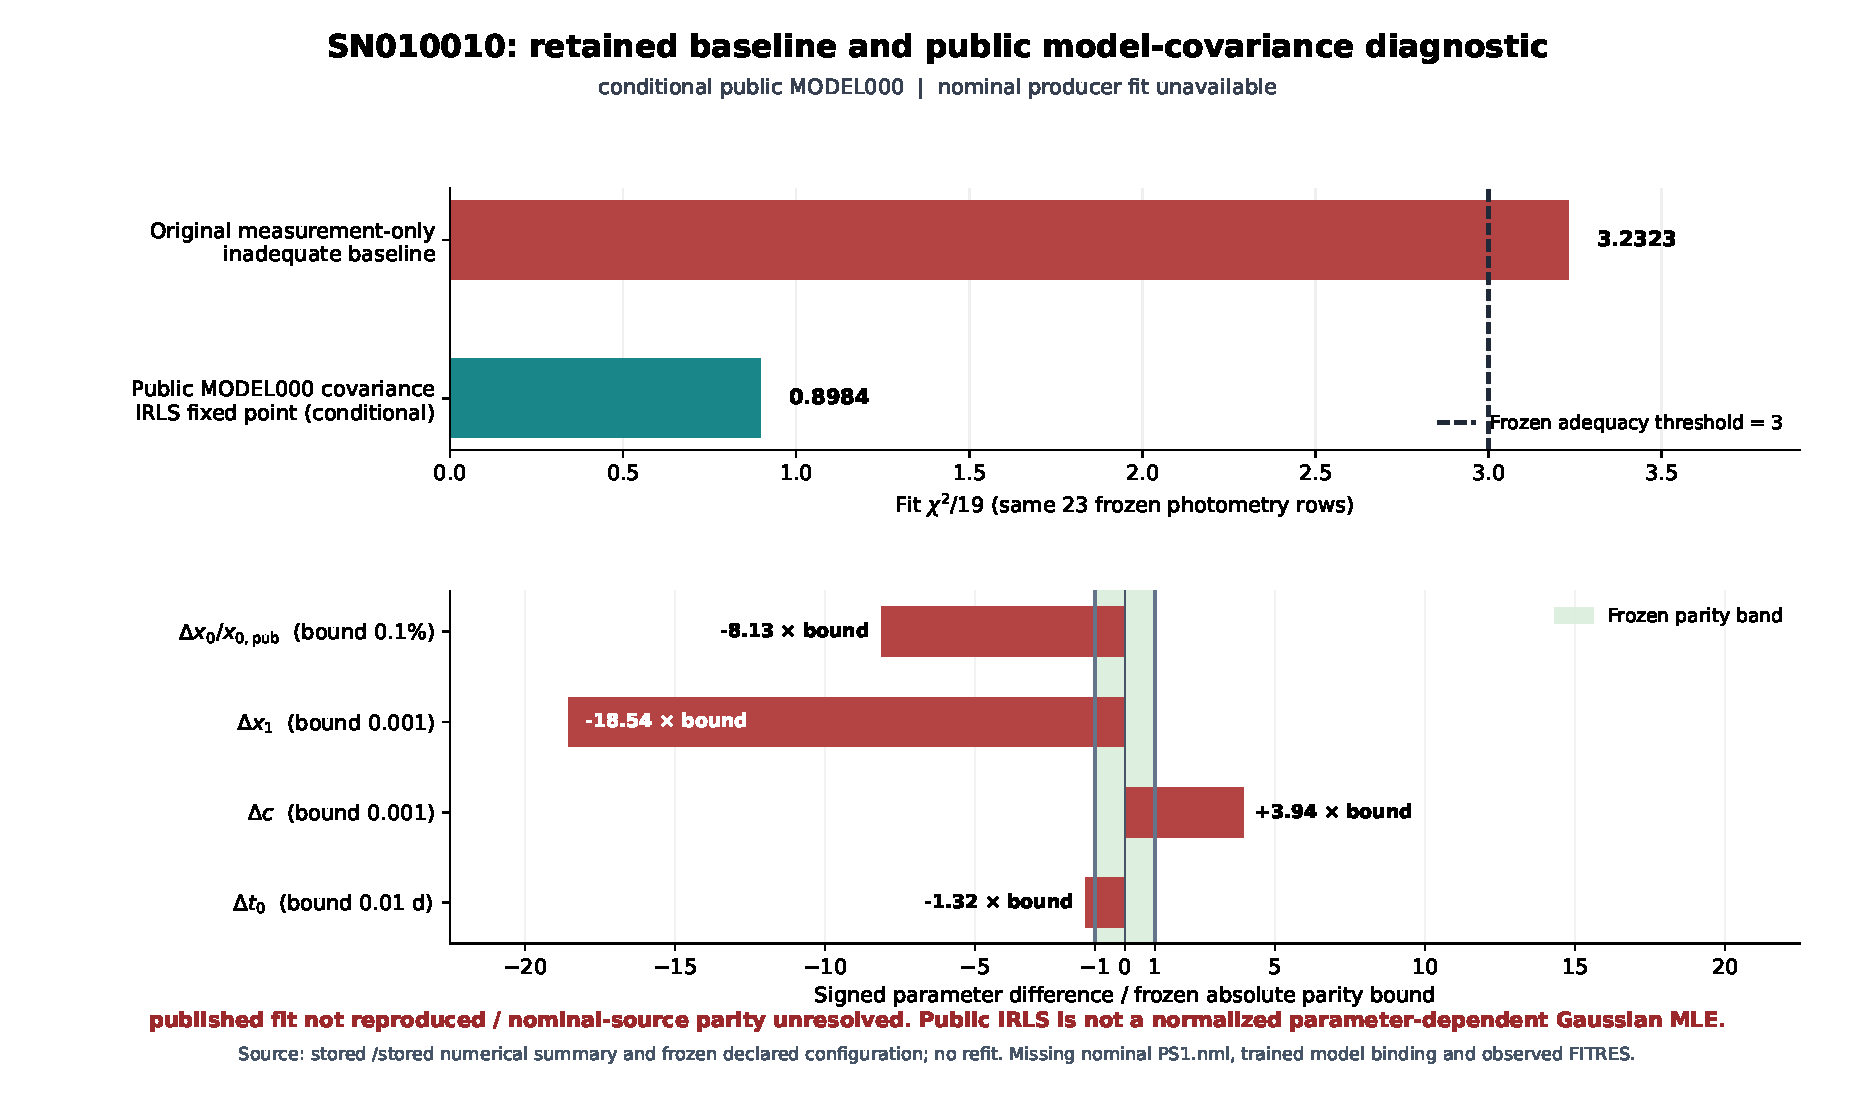
\includegraphics[width=\linewidth,height=.71\textheight,keepaspectratio]{figures/f043_external.pdf}
\caption{SN010010 baseline and public model-covariance comparison. The covariance lowers the conditional residual quadratic, but all stated nominal-summary parity screens fail. The iterated fixed-covariance solution is not the nominal producer fit or a parameter-dependent Gaussian maximum-likelihood fit.}
\label{fig:f043}
\end{figure}
\clearpage
\begin{figure}[p]
\centering
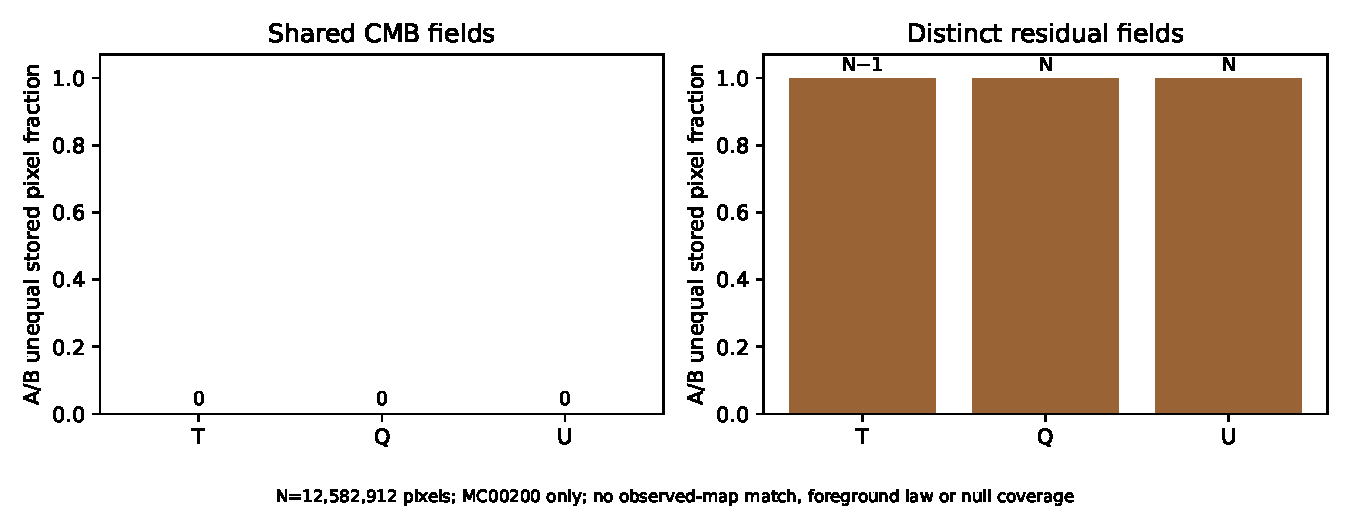
\includegraphics[width=\linewidth,height=.71\textheight,keepaspectratio]{figures/f044.pdf}
\caption{One retained Planck PR4 simulation quartet. Shared CMB fields and distinct residual fields are checked at their original pixels. Identity of the common field is not a joint half-mission source-law qualification or an ensemble noise-covariance estimate.}
\label{fig:f044}
\end{figure}
\clearpage
\begin{figure}[p]
\centering
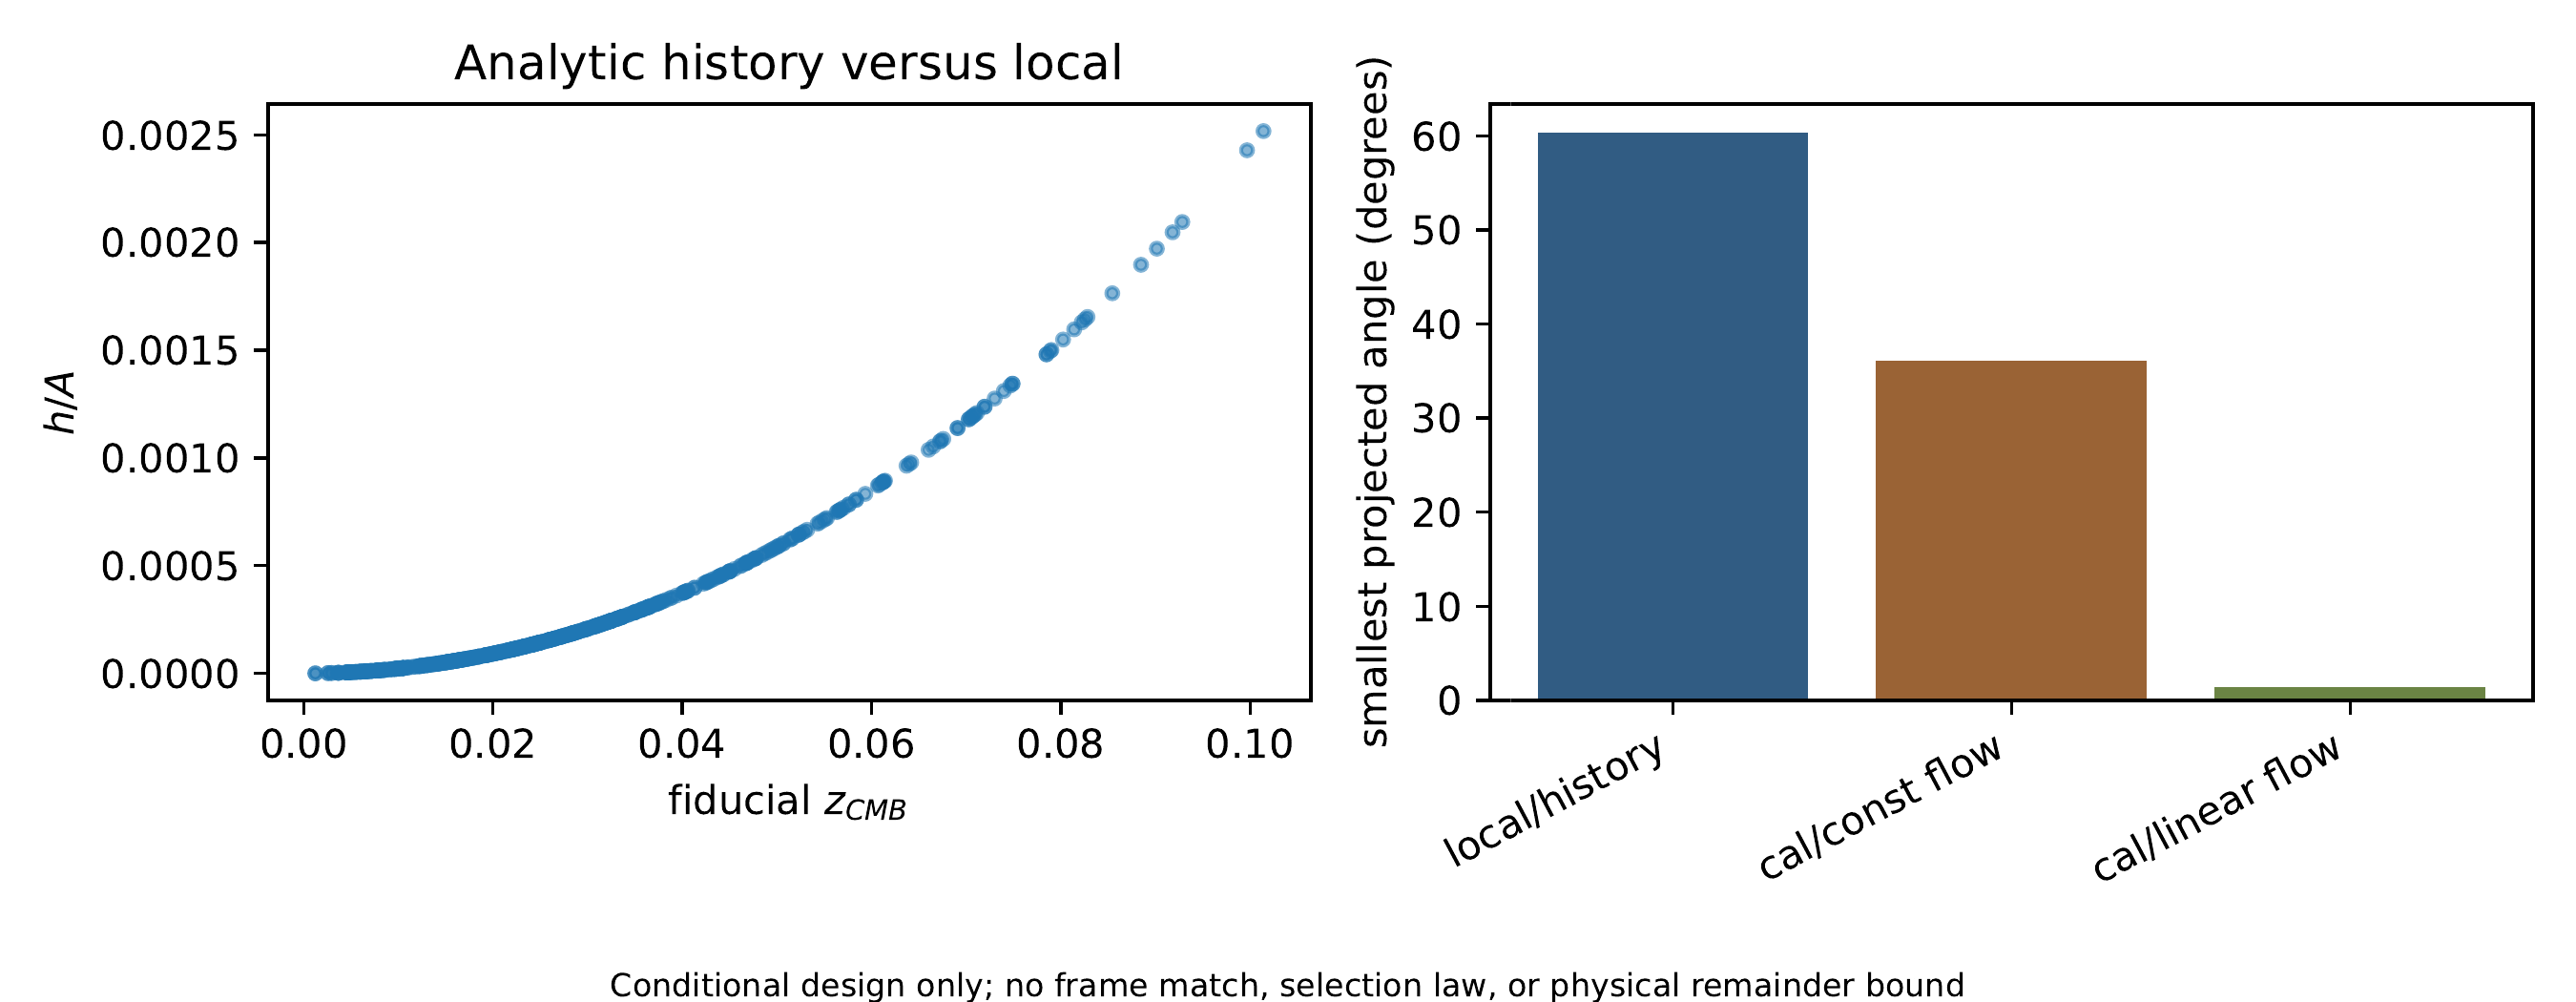
\includegraphics[width=\linewidth,height=.71\textheight,keepaspectratio]{figures/f045_external.png}
\caption{Nuisance-projected response geometry for the retained Pantheon+ and Cosmicflows comparison. The angular and distance-response columns have different principal-angle separation after the specified calibration and dipole projections. The plotted source geometry is conditional on those columns and weights; it does not establish the physical response, joint covariance, or useful discrimination power.}
\label{fig:f045}
\end{figure}
\clearpage
\begin{figure}[p]
\centering
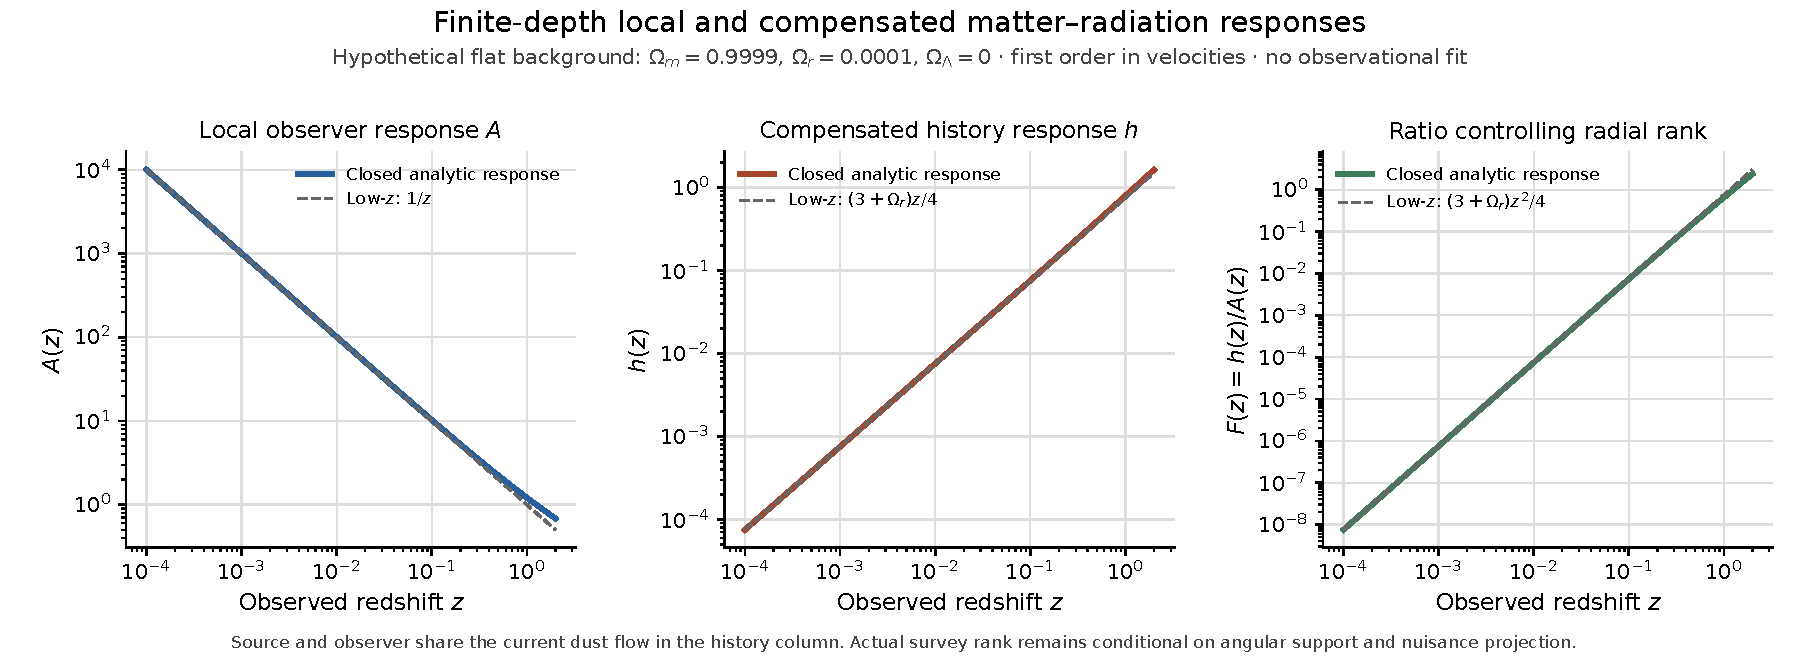
\includegraphics[width=\linewidth,height=.71\textheight,keepaspectratio]{figures/f046.pdf}
\caption{Analytic local-observer and compensated matter--radiation responses in a specified hypothetical background, to first order in velocities. Nonproportional depth dependence can permit conditional discrimination. No observational fit, finite-redshift remainder measurement, or general cosmological response follows.}
\label{fig:f046}
\end{figure}
\clearpage
\begin{figure}[p]
\centering
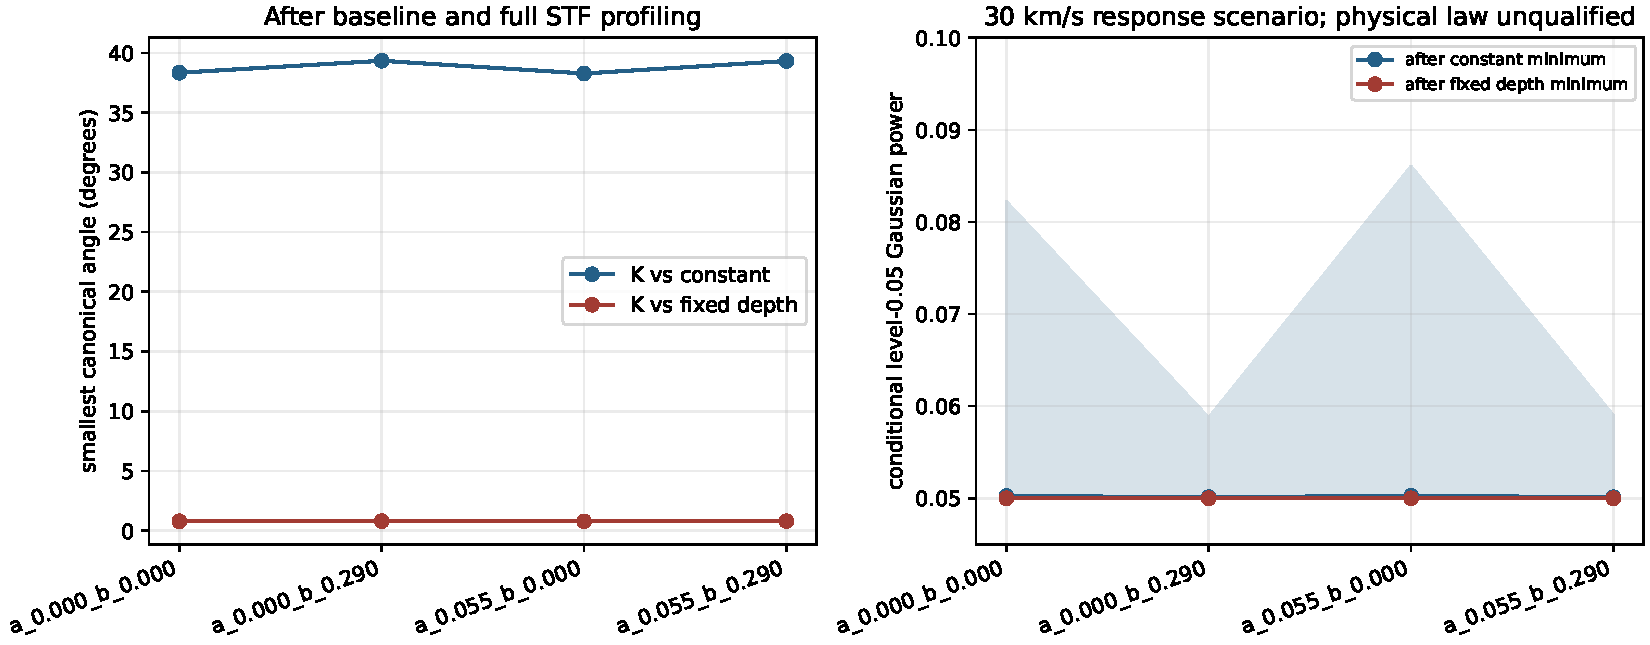
\includegraphics[width=\linewidth,height=.71\textheight,keepaspectratio]{figures/f047_external.pdf}
\caption{Geometry and conditional power of inverse-velocity, constant-calibration, and polynomial-depth vector responses on the retained distance cohort. The broader depth nuisance nearly absorbs the inverse-velocity response. These are selected-design calculations; the low-speed physical expansion and acceleration interpretation remain unqualified.}
\label{fig:f047}
\end{figure}
\clearpage
\begin{figure}[p]
\centering
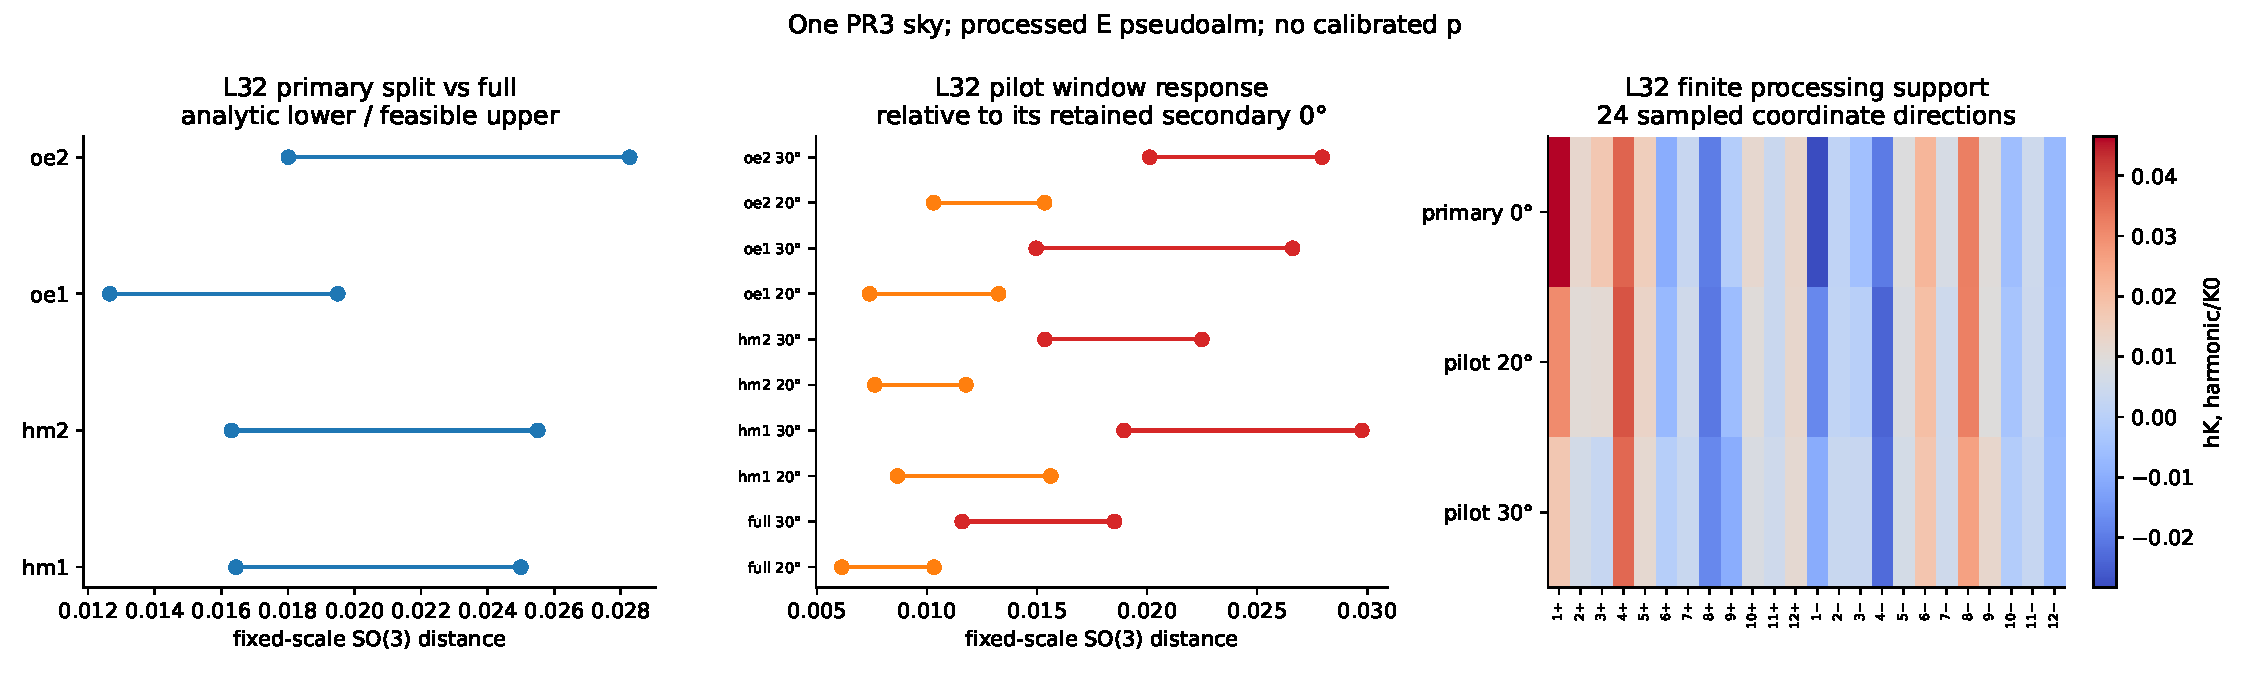
\includegraphics[width=\linewidth,height=.71\textheight,keepaspectratio]{figures/f050_external.pdf}
\caption{Proper-rotation orbit enclosures and sampled directional supports for the complete processed E quadrupole and octupole of one Planck sky. Lower bounds use invariants; upper bounds use feasible rotations. The finite supports describe convex-hull projections, not a physical confidence set or complete nonconvex morphology.}
\label{fig:f050}
\end{figure}
\clearpage
\begin{figure}[p]
\centering
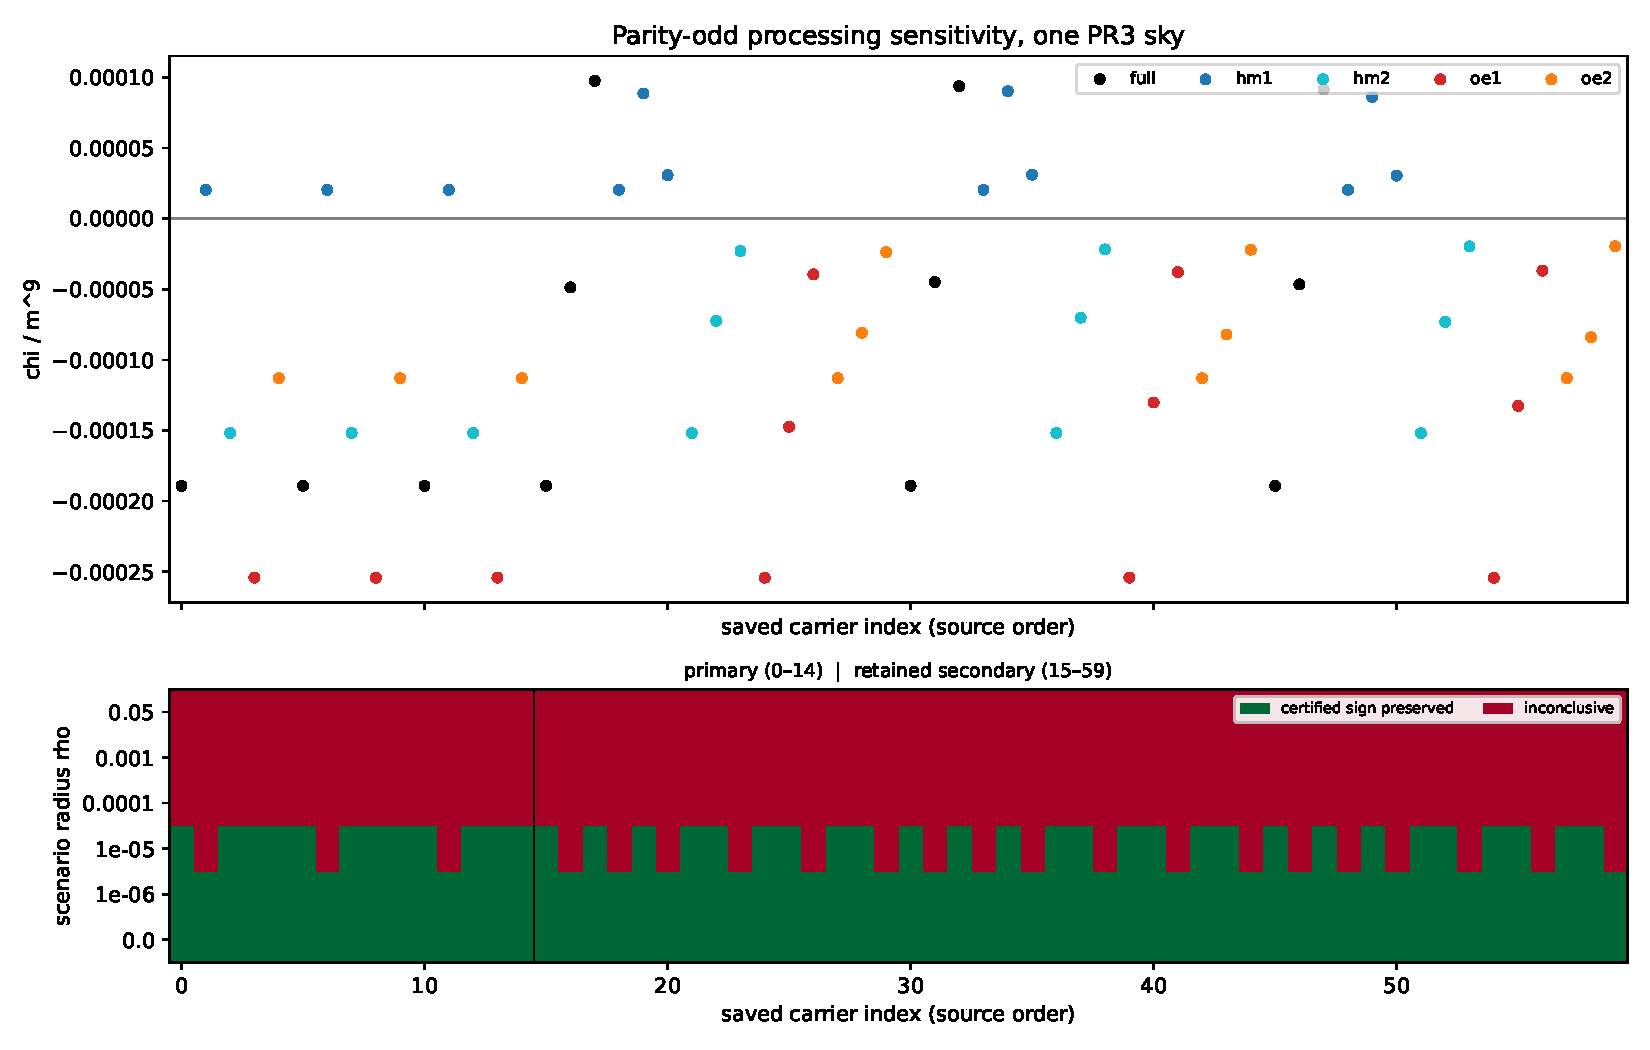
\includegraphics[width=\linewidth,height=.71\textheight,keepaspectratio]{figures/f051_external.pdf}
\caption{Proper-rotation chirality of sixty exact finite processed E tensor carriers and its sensitivity to declared tensor radii. Nonzero signs distinguish each stored carrier from its mirror under proper rotations. The radii are not measured errors, and no primordial parity violation or null significance is inferred.}
\label{fig:f051}
\end{figure}
\clearpage
\begin{figure}[p]
\centering
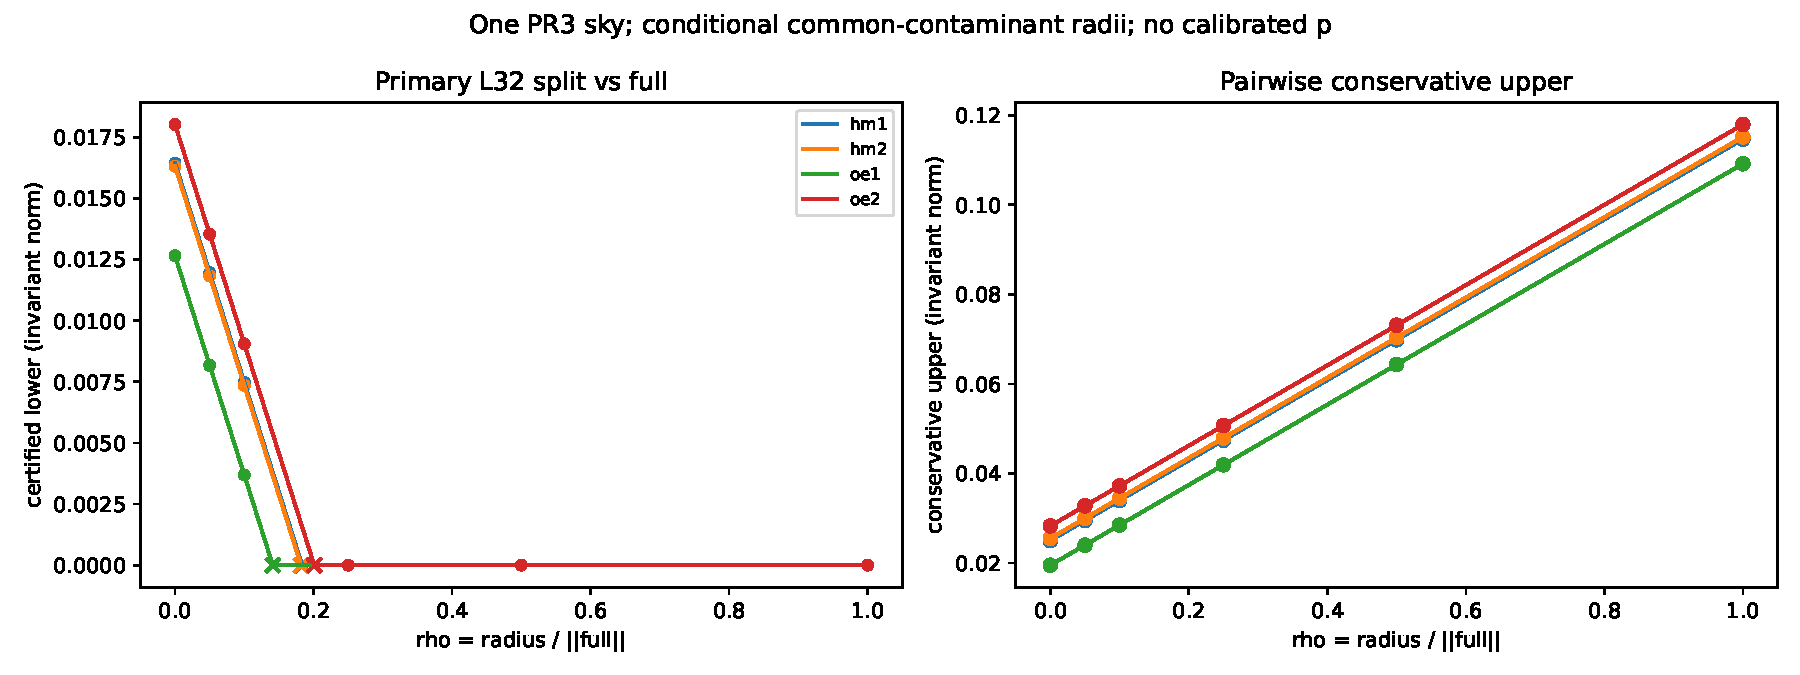
\includegraphics[width=\linewidth,height=.71\textheight,keepaspectratio]{figures/f052.pdf}
\caption{Conservative orbit-distance widening under common-contaminant radius scenarios. A lower certificate reaching zero means that this certificate no longer discriminates. It does not prove equality of the true tensors; common contamination and split cross-noise are not calibrated.}
\label{fig:f052}
\end{figure}
\clearpage
\begin{figure}[p]
\centering
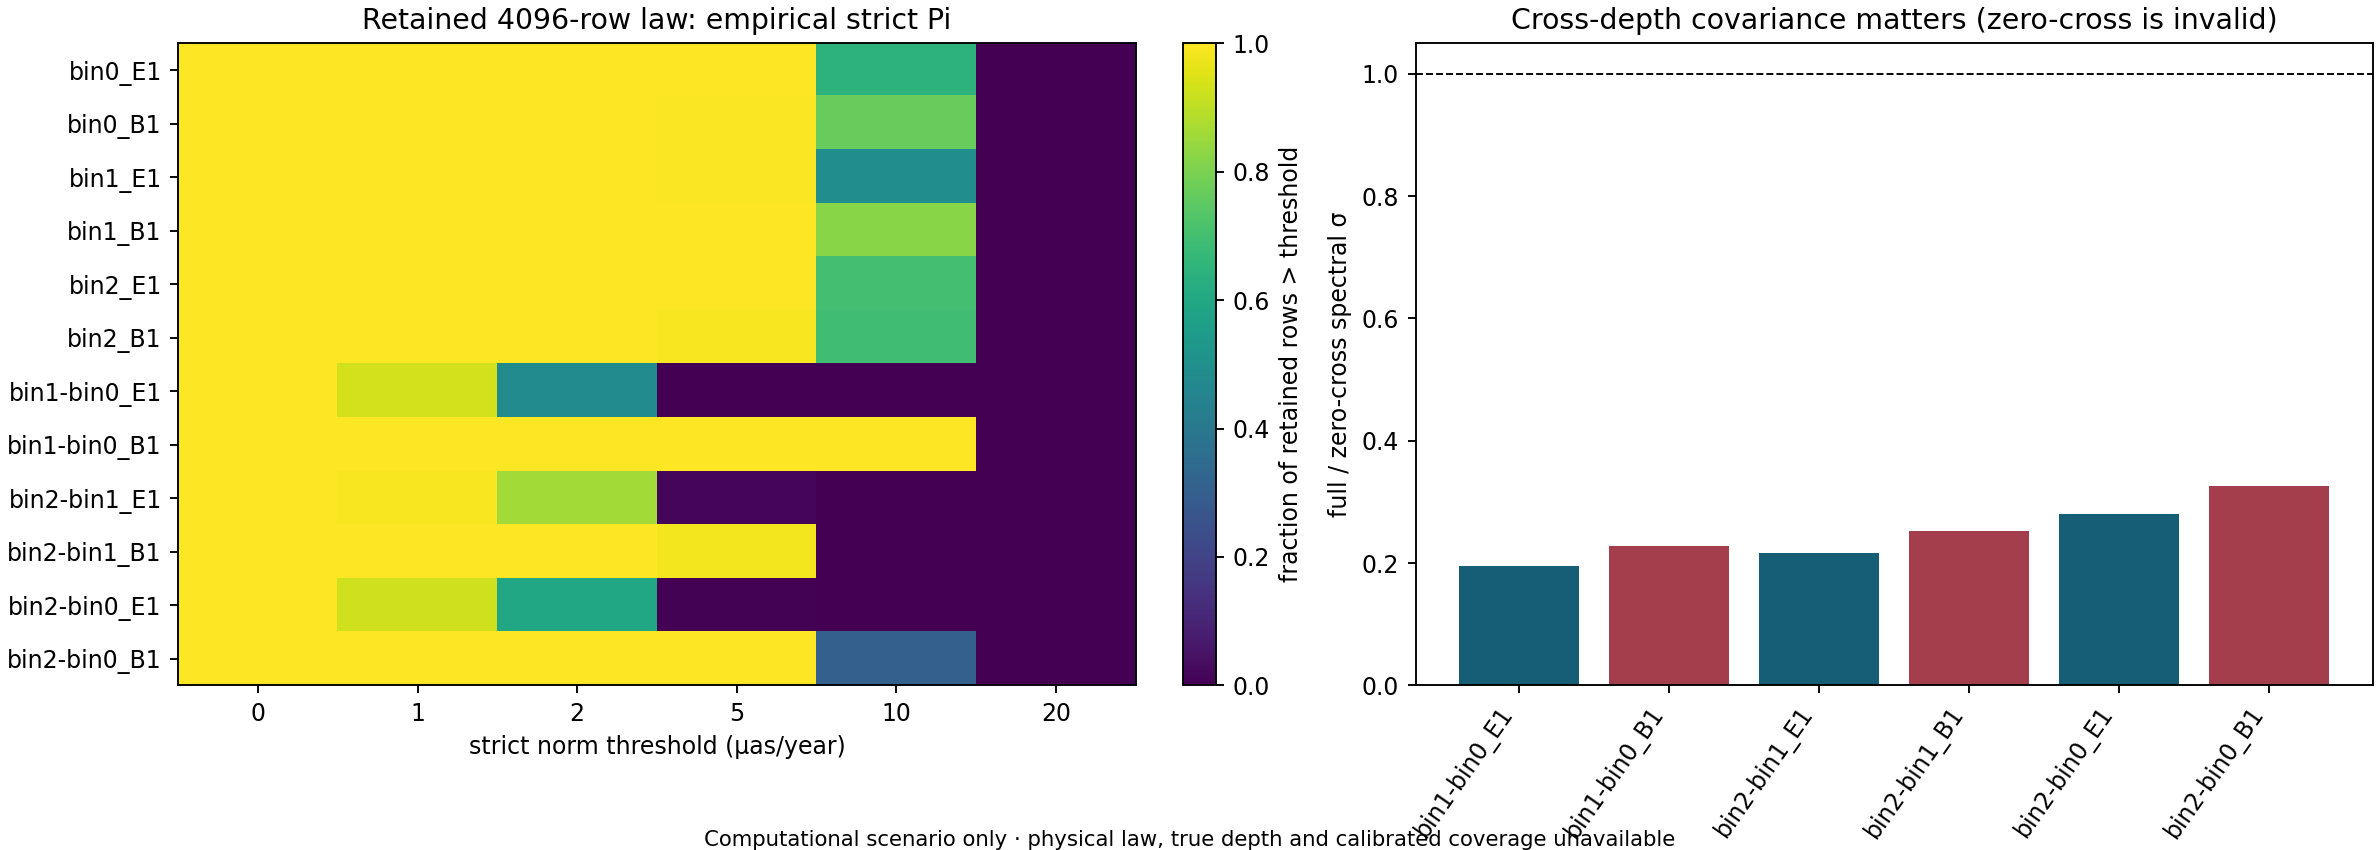
\includegraphics[width=\linewidth,height=.71\textheight,keepaspectratio]{figures/f054.png}
\caption{Strict empirical exceedances and cross-depth covariance effects for the same 4096 joint astrometric rows. The corrected reported-bin map includes the shared slope. Removing covariance is a counterfactual diagnostic; finite frequencies are not physical probabilities.}
\label{fig:f054}
\end{figure}
\clearpage
\begin{figure}[p]
\centering
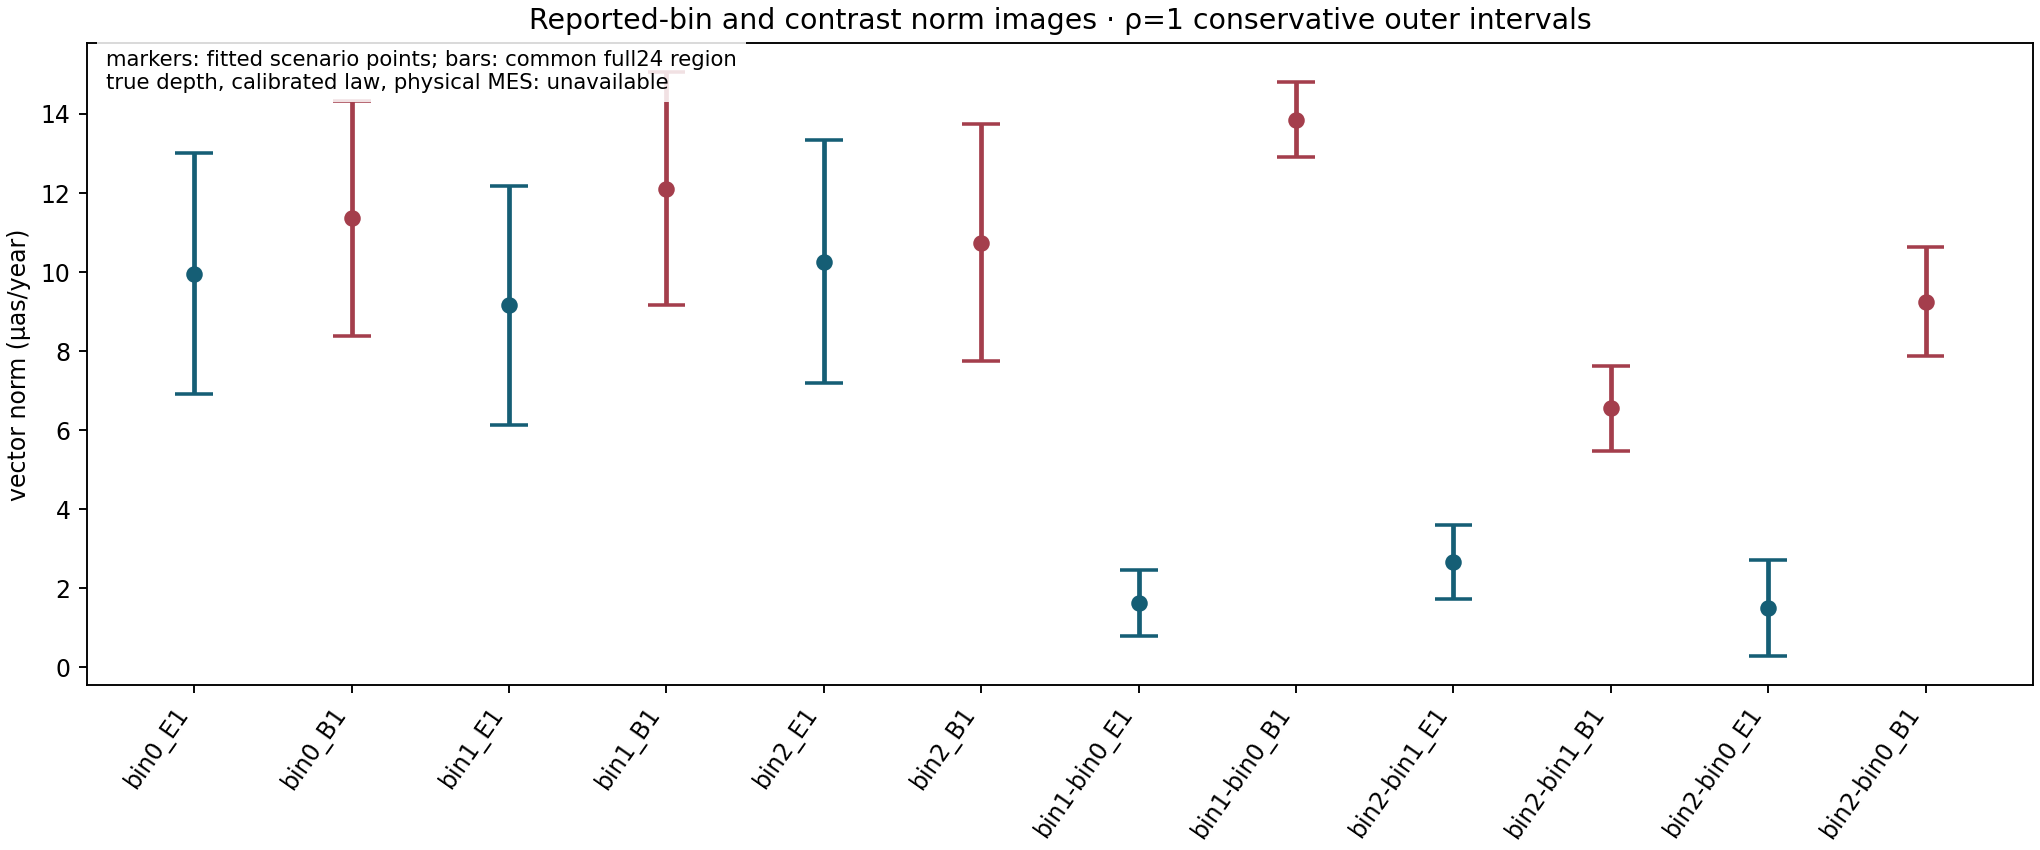
\includegraphics[width=\linewidth,height=.71\textheight,keepaspectratio]{figures/f055.png}
\caption{Full-covariance functional depth images of the astrometric state, with reported-bin values and contrasts. Coordinate support is exact under the declared joint region; norm bars are conservative outer bounds. True-depth response and physical coverage remain unqualified.}
\label{fig:f055}
\end{figure}
\clearpage
\begin{figure}[p]
\centering
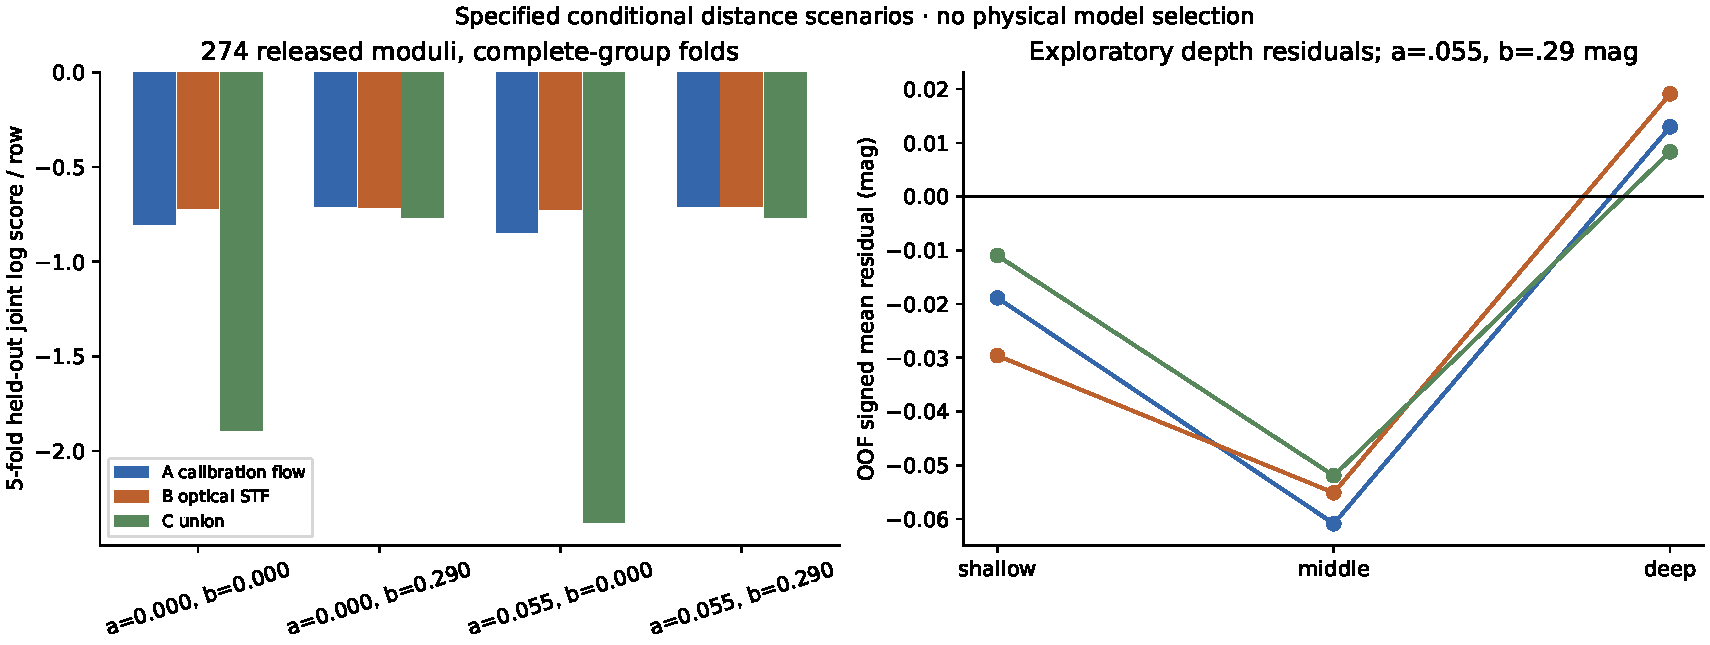
\includegraphics[width=\linewidth,height=.71\textheight,keepaspectratio]{figures/f058_external.pdf}
\caption{Whole-group held-out distance prediction and signed residual summaries. The model ranking changes with the declared group-covariance scenario. All scenarios use the same observed cohort; the plots do not validate a physical calibration, flow, or shear interpretation.}
\label{fig:f058}
\end{figure}
\clearpage
\begin{figure}[p]
\centering
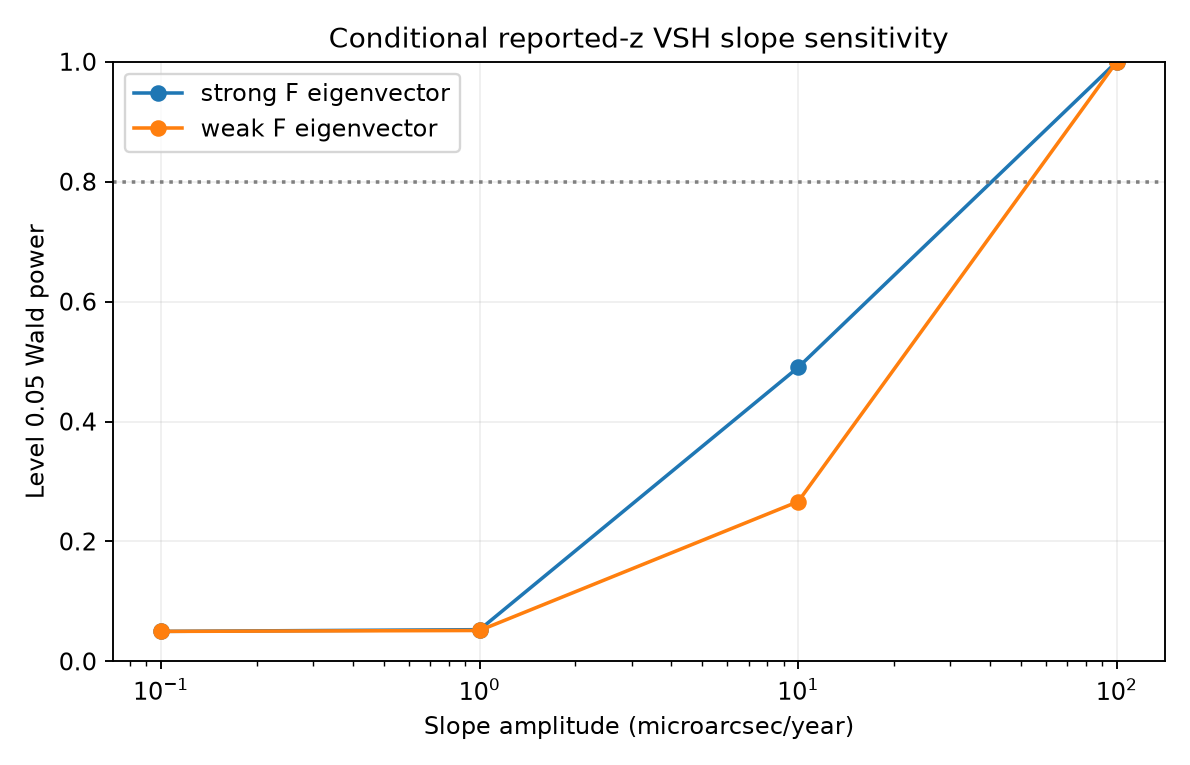
\includegraphics[width=\linewidth,height=.71\textheight,keepaspectratio]{figures/f059.png}
\caption{Continuous reported-redshift slope response after profiling the full astrometric nuisance design. The power curves and errors use the independent-row reported-covariance Gaussian working law. They are conditional design quantities, not empirical physical limits.}
\label{fig:f059}
\end{figure}
\clearpage
\begin{figure}[p]
\centering
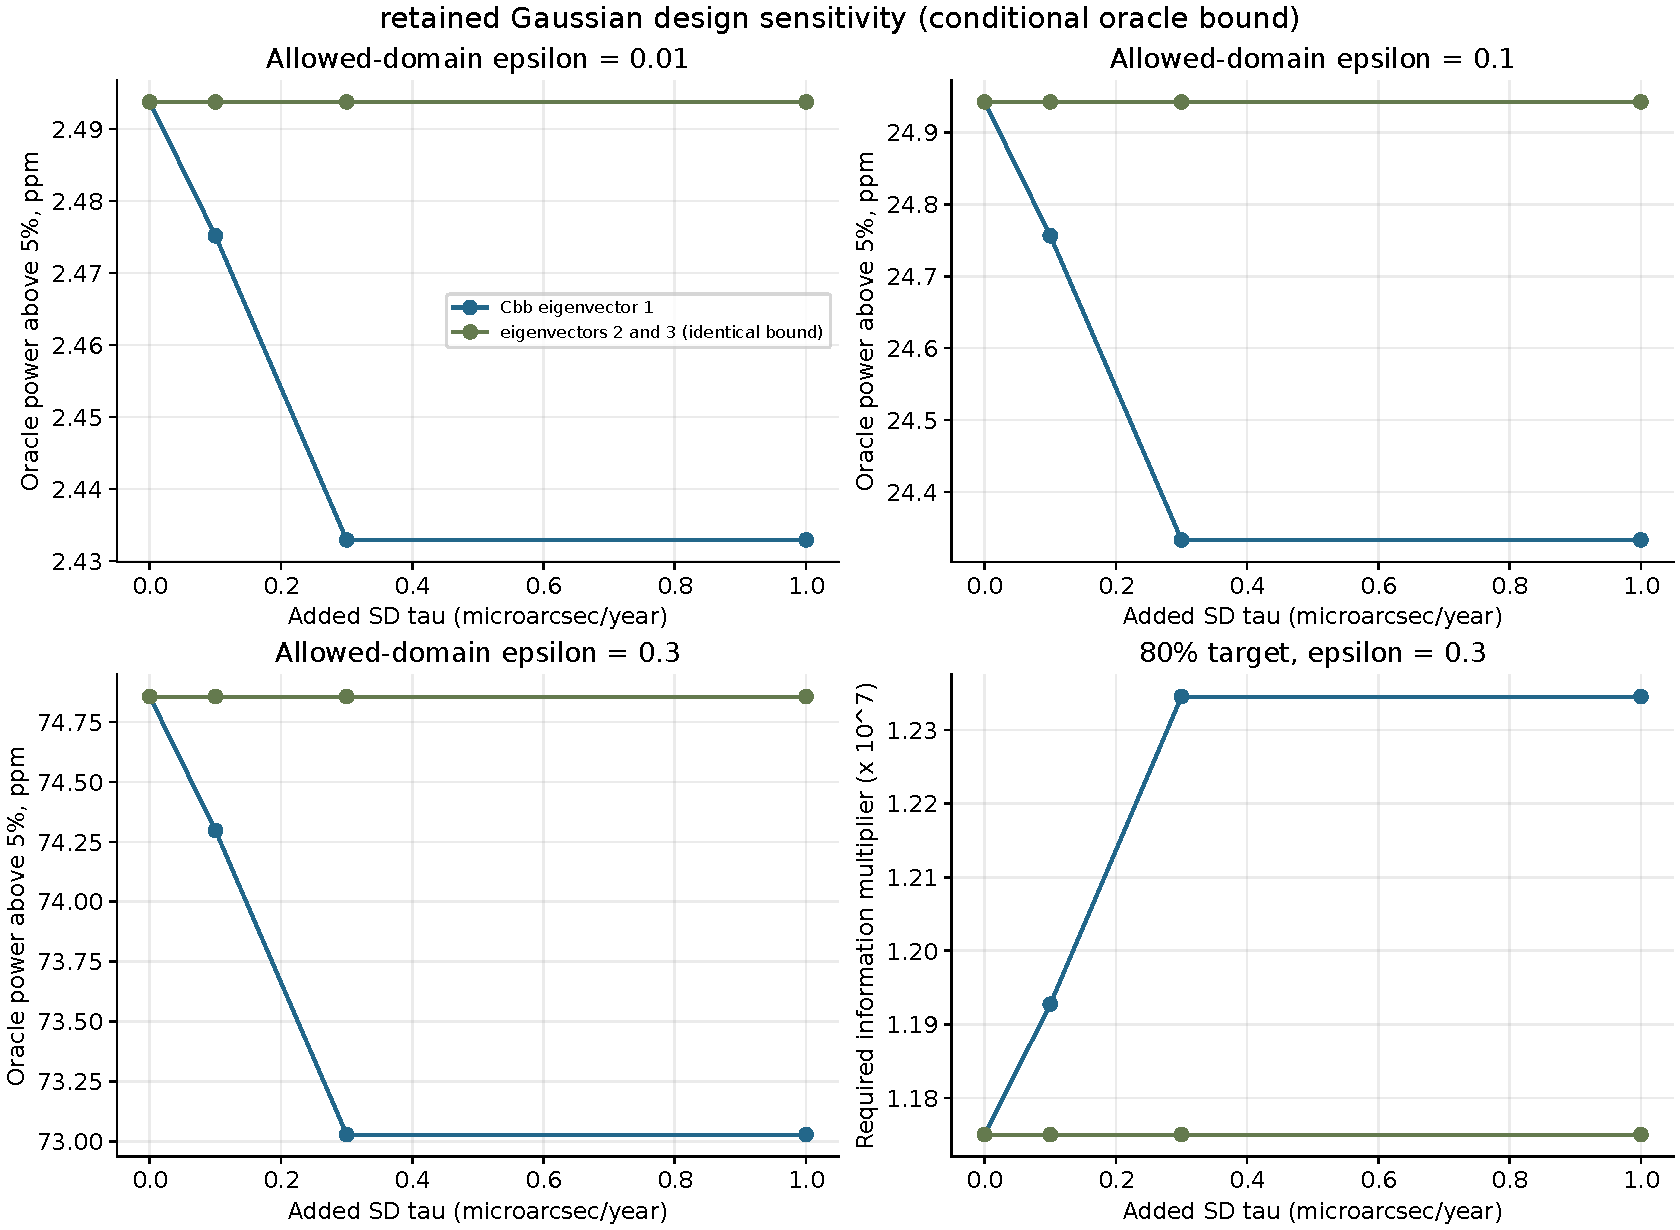
\includegraphics[width=\linewidth,height=.71\textheight,keepaspectratio]{figures/f060_external.pdf}
\caption{Oracle power sensitivity for the retained profiled astrometric history covariance. The allowed-domain parameter and added covariance are scenarios. Information multipliers are requirements within the fixed response model, not demonstrated observing-program improvements.}
\label{fig:f060}
\end{figure}
\clearpage
\begin{figure}[p]
\centering
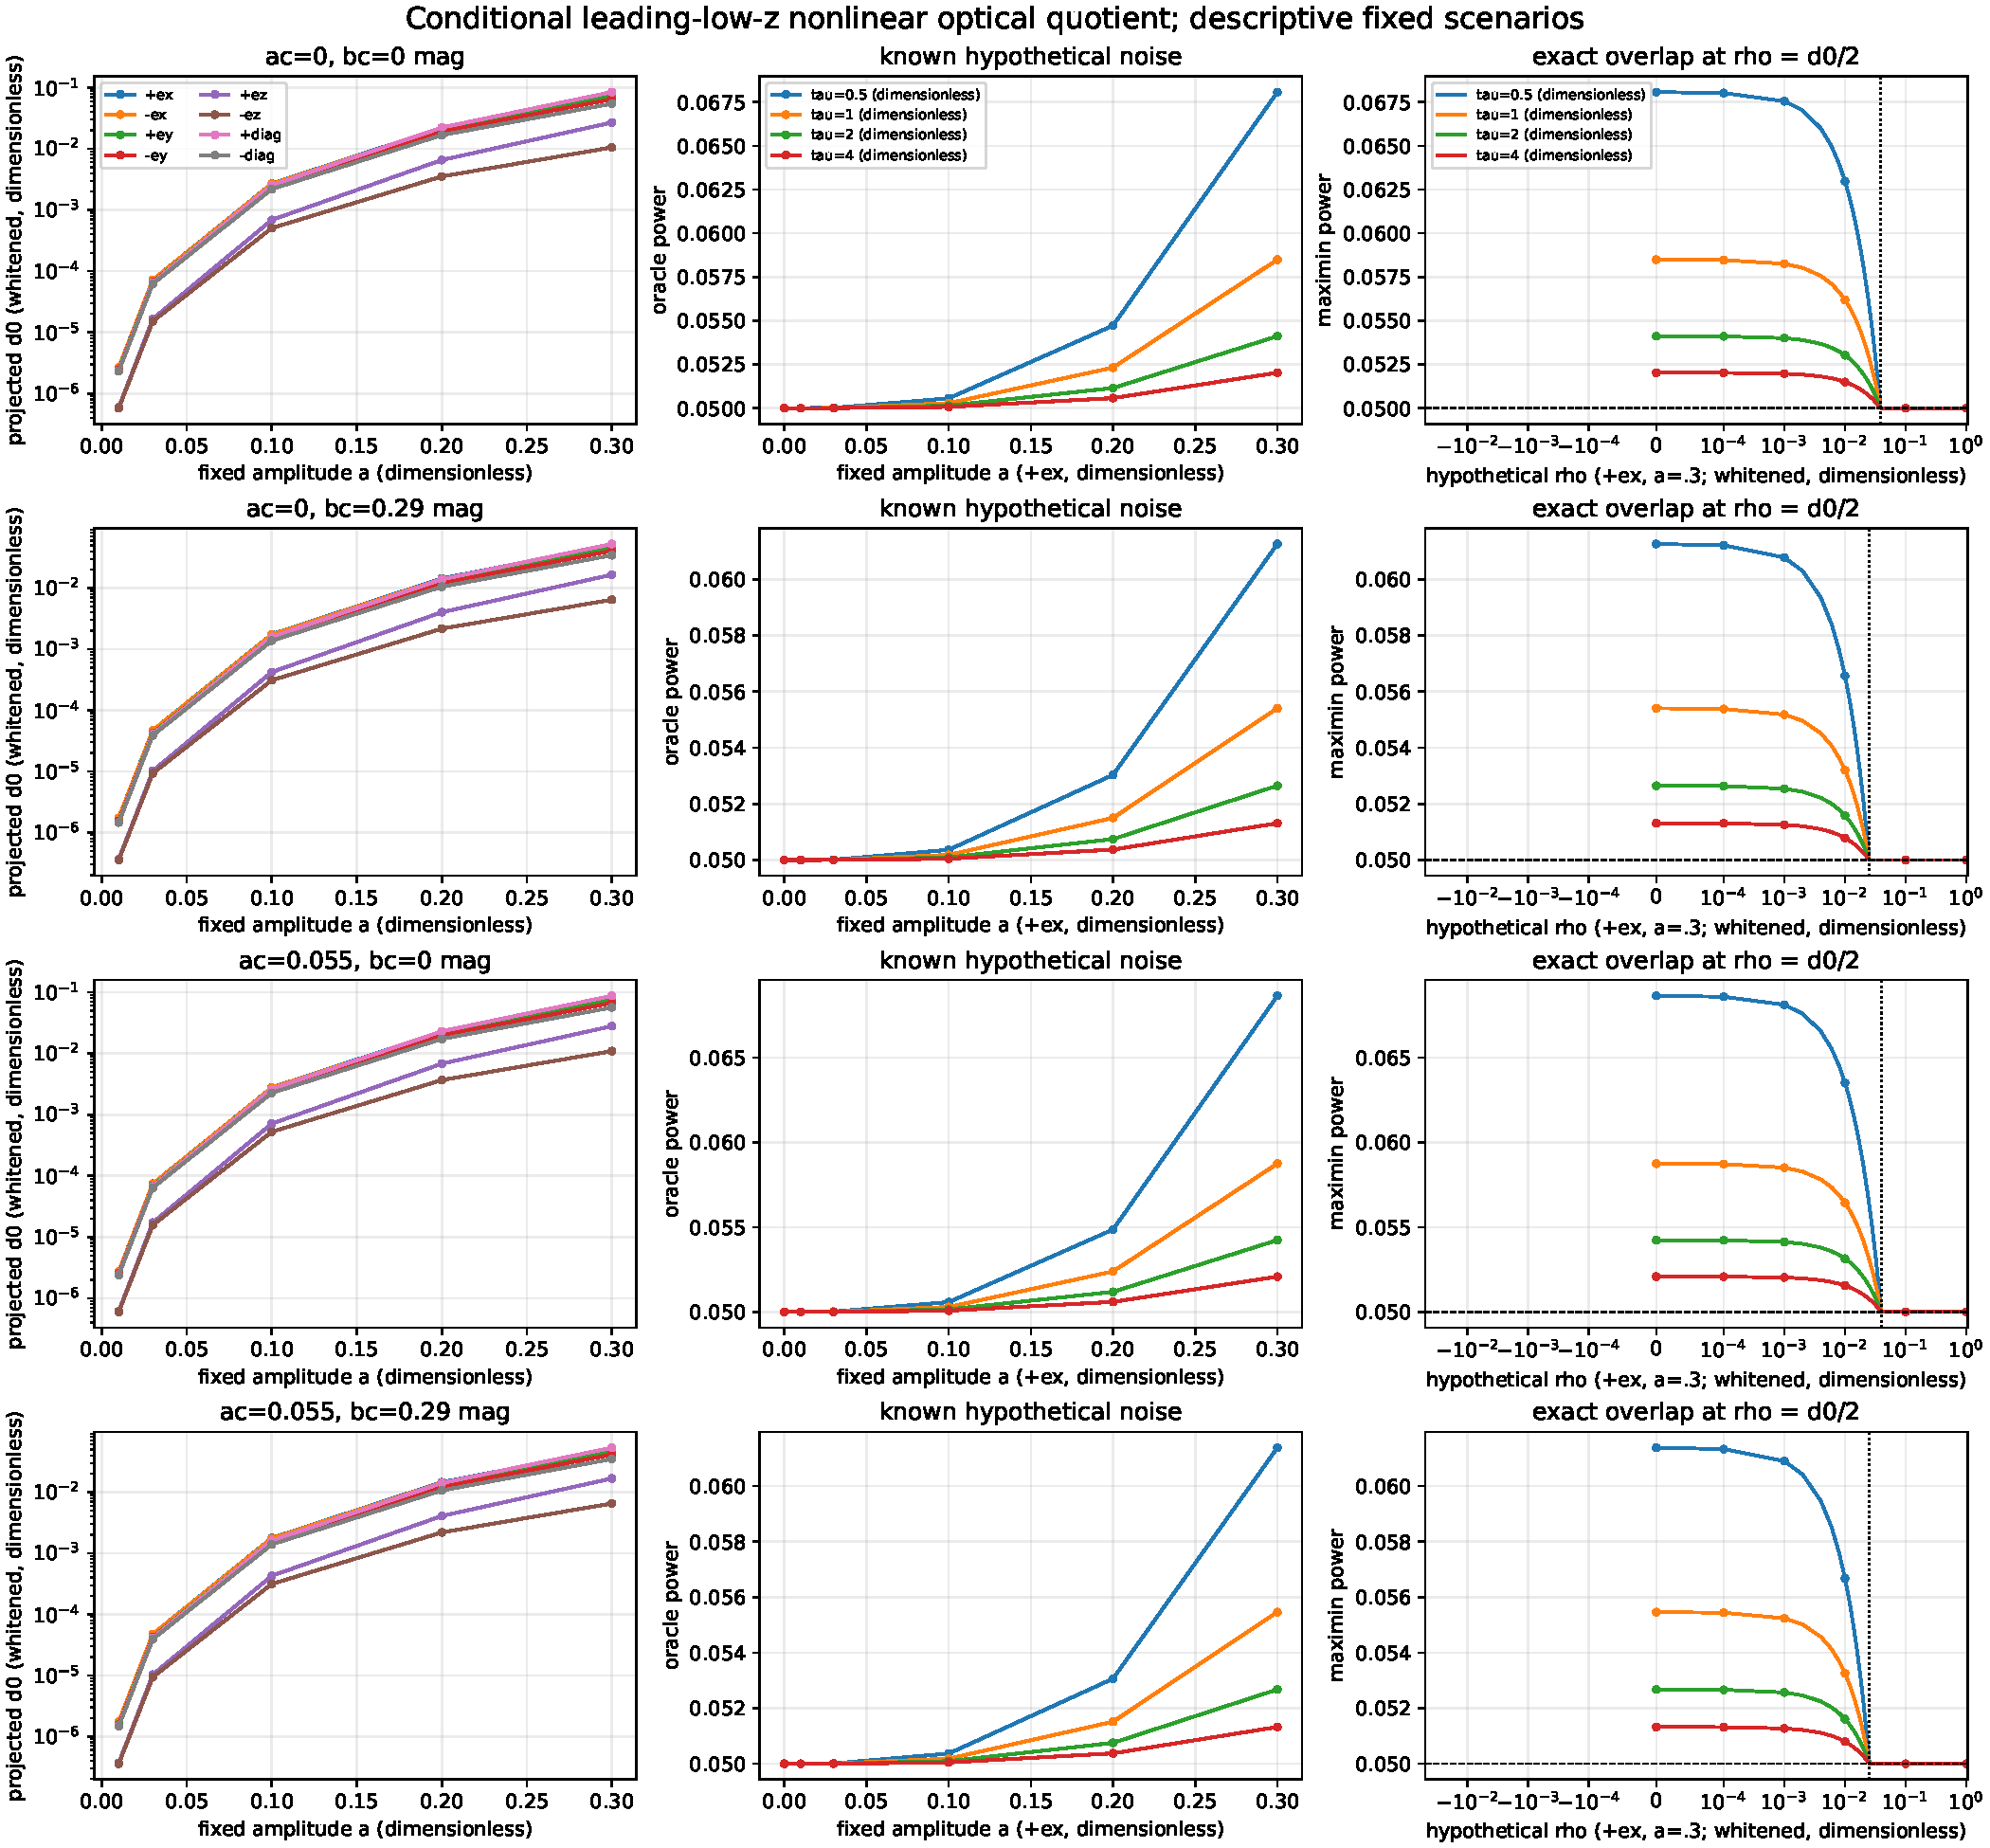
\includegraphics[width=\linewidth,height=.71\textheight,keepaspectratio]{figures/f061.pdf}
\caption{Nonlinear optical response after quotienting the fitted baseline, dipole, and STF space. All directions and amplitudes are fixed scenarios. The remainder curves include the exact overlap radius; beyond overlap the conditional benchmark is the test size. Finite-redshift physical remainder is unmeasured.}
\label{fig:f061}
\end{figure}
\clearpage
\begin{figure}[p]
\centering
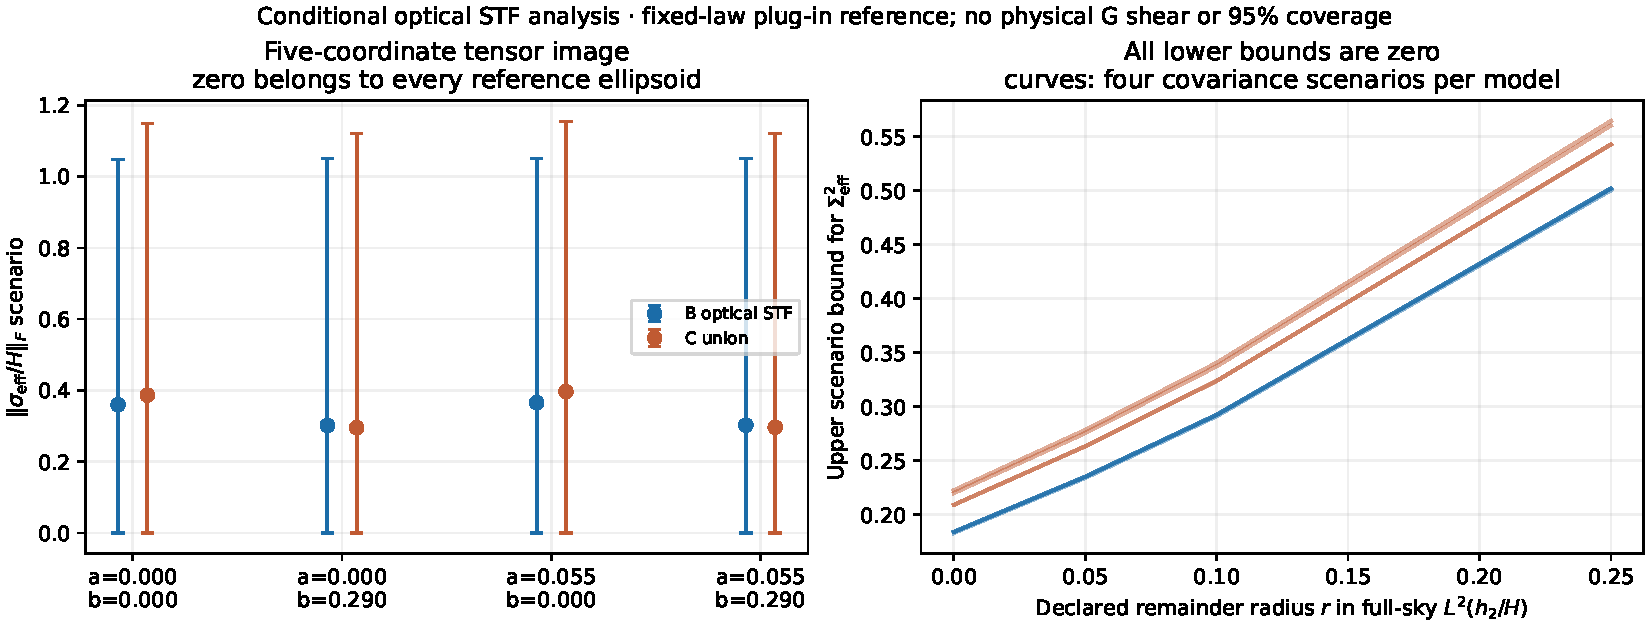
\includegraphics[width=\linewidth,height=.71\textheight,keepaspectratio]{figures/f063.pdf}
\caption{Full-covariance optical STF images of the selected distance fits. Every reference ellipsoid permits zero quadrupole. The effective-shear conversion is a linearized fixed-redshift scenario; its reference region and added remainder radii do not measure local congruence shear or physical coverage.}
\label{fig:f063}
\end{figure}
\clearpage
\begin{figure}[p]
\centering
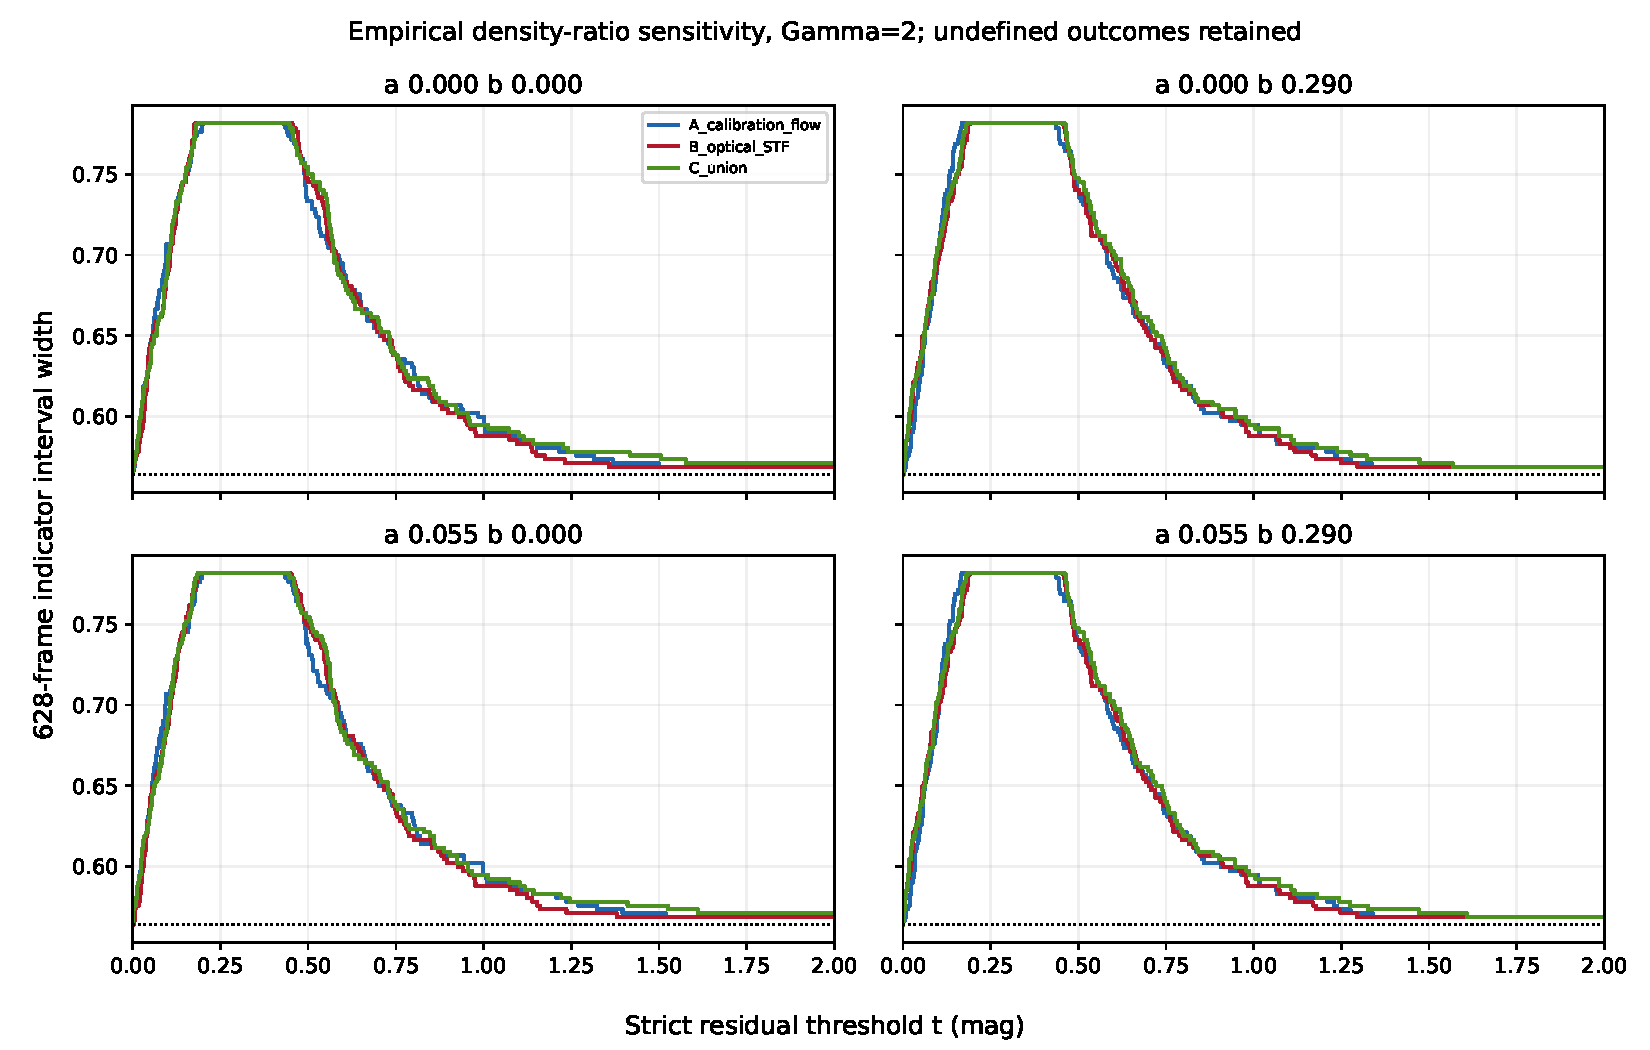
\includegraphics[width=\linewidth,height=.71\textheight,keepaspectratio]{figures/f064.pdf}
\caption{Sharp empirical density-ratio sensitivity followed by unrestricted completion of missing target events. The total interval width retains the missing fraction. These are finite-target event bounds, not estimated parent propensities or a probability of cosmological geometry.}
\label{fig:f064}
\end{figure}
\clearpage
\begin{figure}[p]
\centering
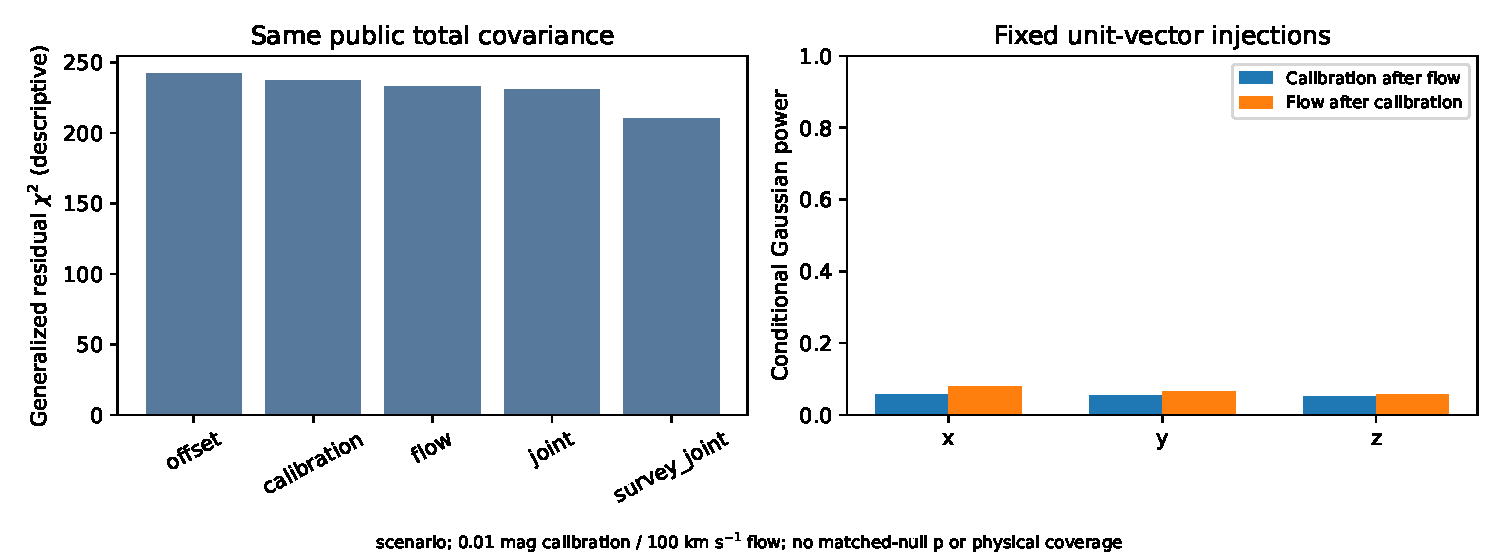
\includegraphics[width=\linewidth,height=.71\textheight,keepaspectratio]{figures/f065_external.pdf}
\caption{Pantheon+ conditional mean-model comparison using the released total covariance once. The residual quadratics are descriptive, and the injection powers use a fixed Gaussian reference. Calibration and frozen-flow coefficient blocks remain correlated; nominal-source parity and cross-survey covariance are not supplied.}
\label{fig:f065}
\end{figure}
\clearpage
\begin{figure}[p]
\centering
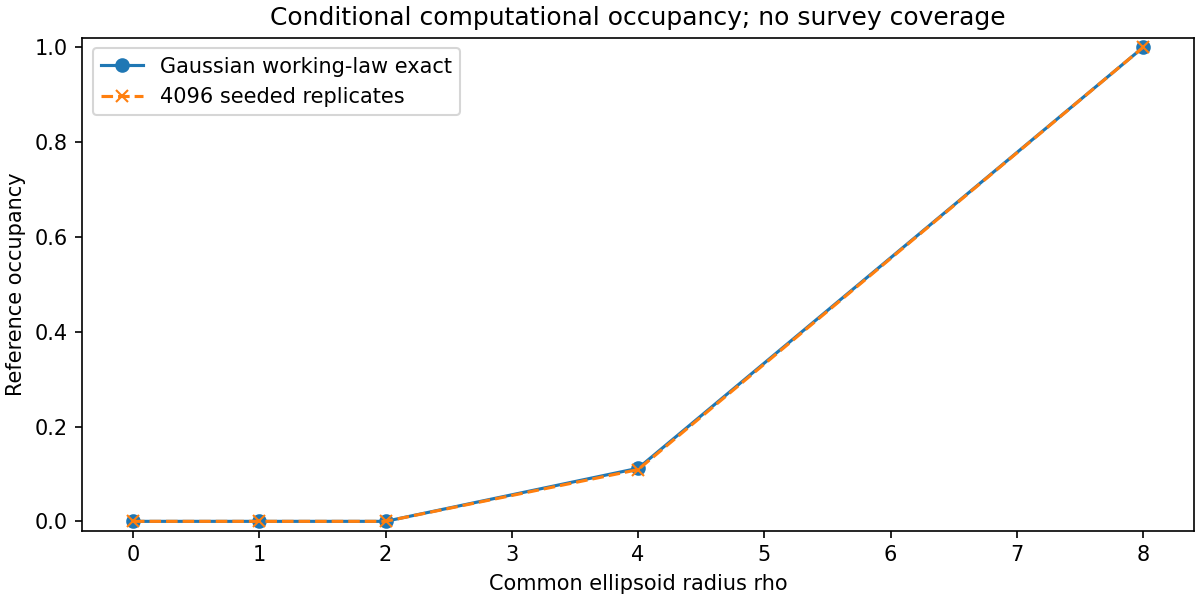
\includegraphics[width=\linewidth,height=.71\textheight,keepaspectratio]{figures/f066.png}
\caption{Occupancy of named computational regions under the stated Gaussian reference and retained joint samples. A reference region is not itself a probability measure. The computational anchor is separate from an unavailable physical bound; no selected-survey coverage is claimed.}
\label{fig:f066}
\end{figure}
\clearpage
\begin{figure}[p]
\centering
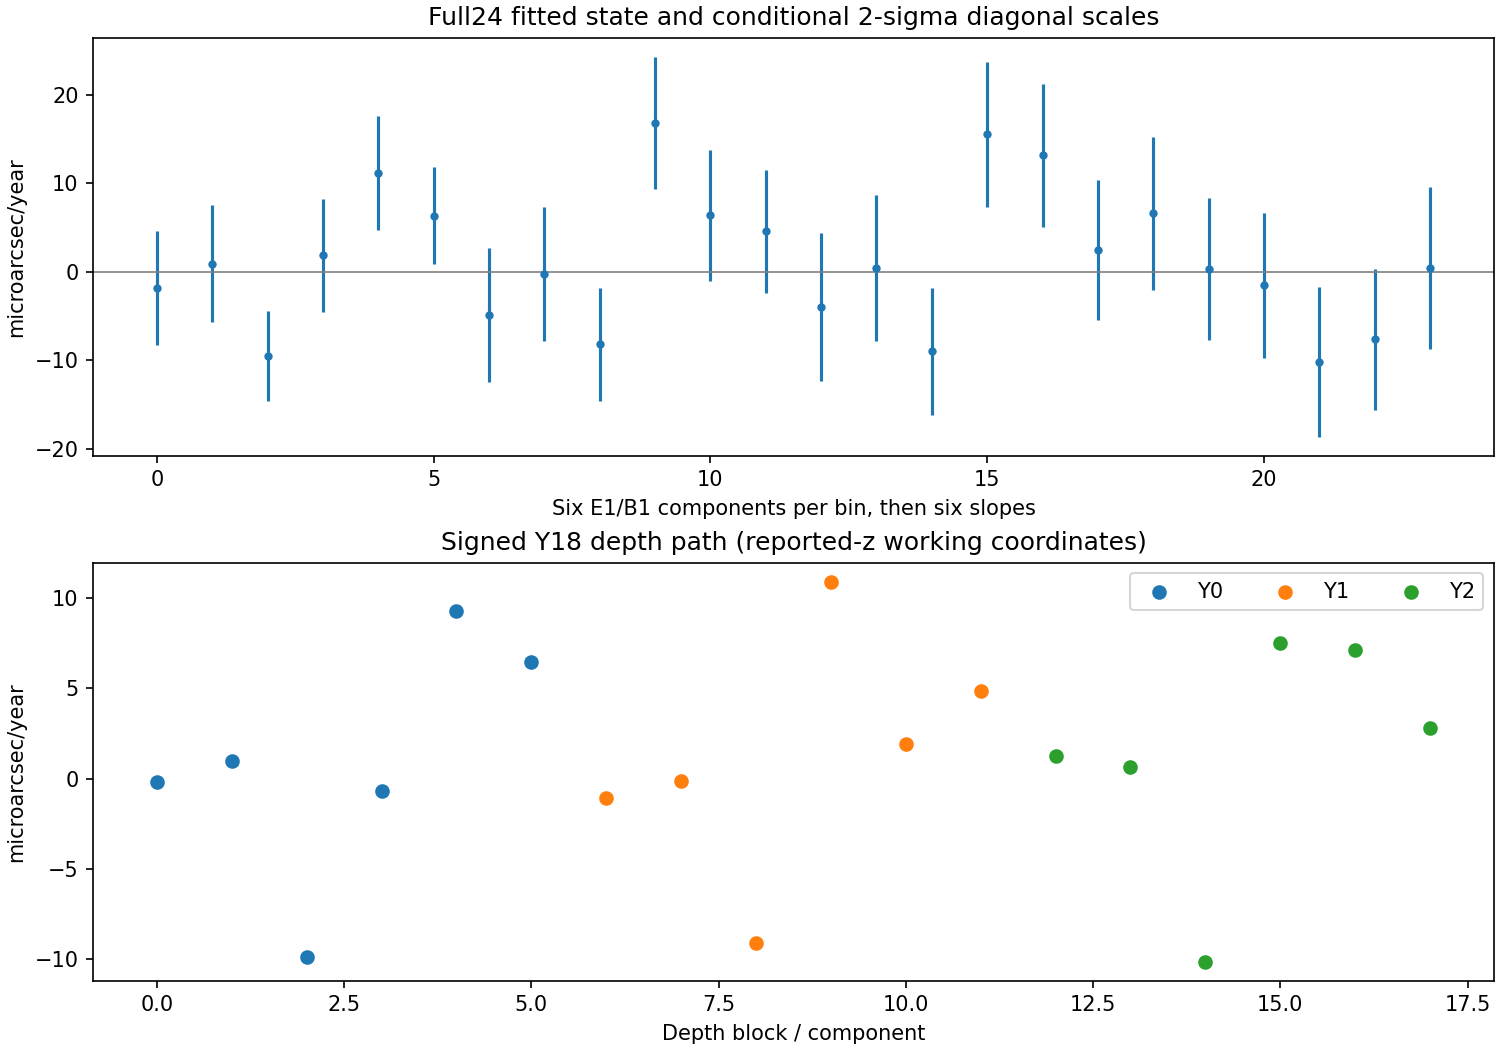
\includegraphics[width=\linewidth,height=.71\textheight,keepaspectratio]{figures/f067.png}
\caption{Full astrometric tensor-state diagnostics with shared covariance and finite empirical exceedance. Polar and axial coordinates and the original state accompany all scalar summaries. The computational norm scale is not a physical anisotropy anchor.}
\label{fig:f067}
\end{figure}
\clearpage
\begin{figure}[p]
\centering
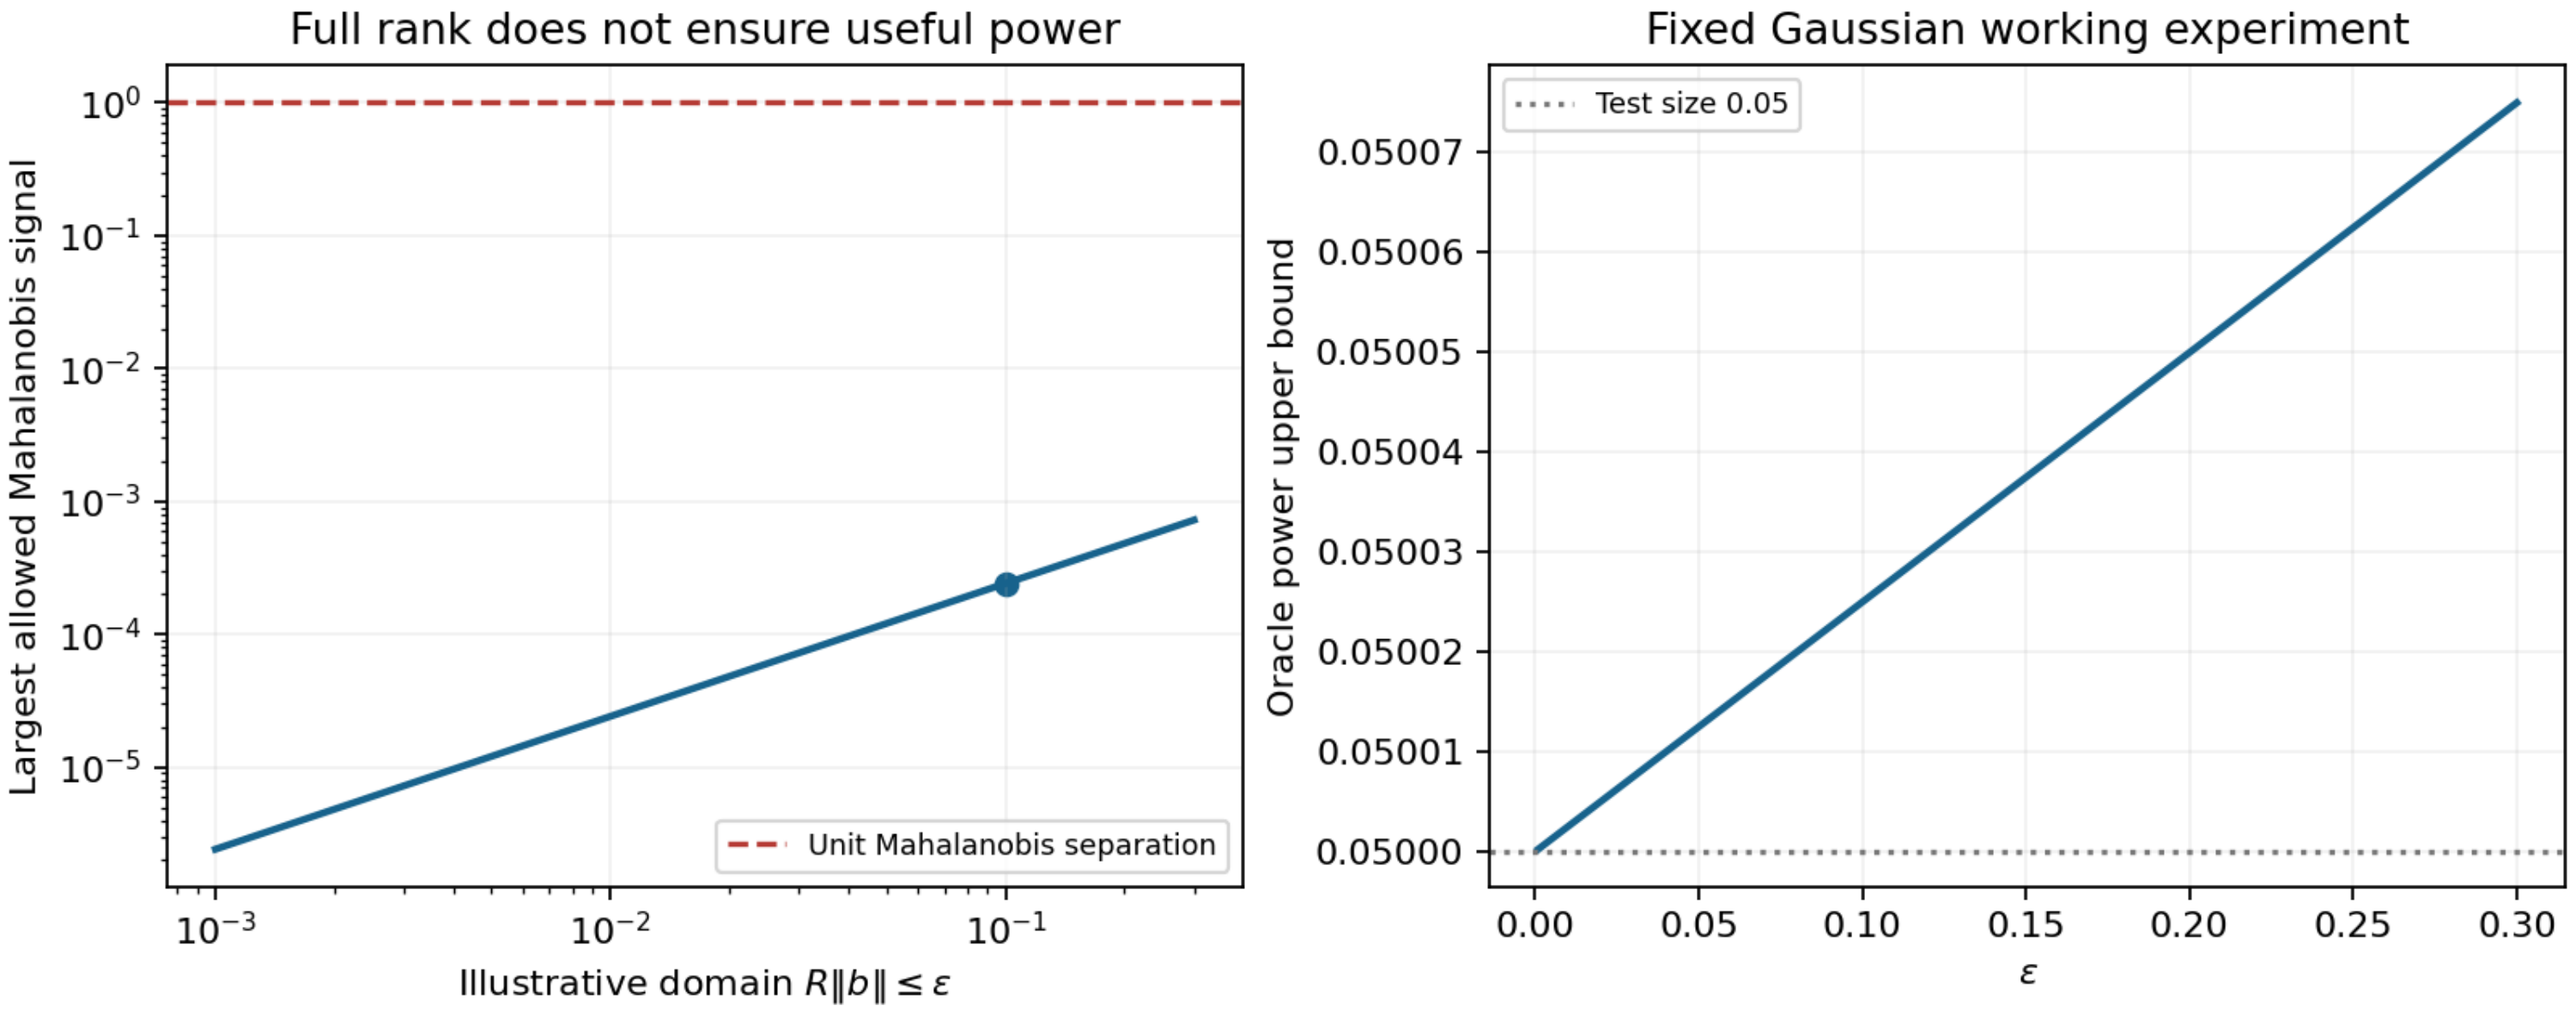
\includegraphics[width=\linewidth,height=.71\textheight,keepaspectratio]{figures/f068_external.png}
\caption{Best-direction Gaussian power in a restricted illustrative history-response domain. Even the oracle bound is close to test size. The restriction controls a stated small parameter; it does not certify every physical remainder or prove a universal observational impossibility.}
\label{fig:f068}
\end{figure}
\clearpage
\begin{figure}[p]
\centering
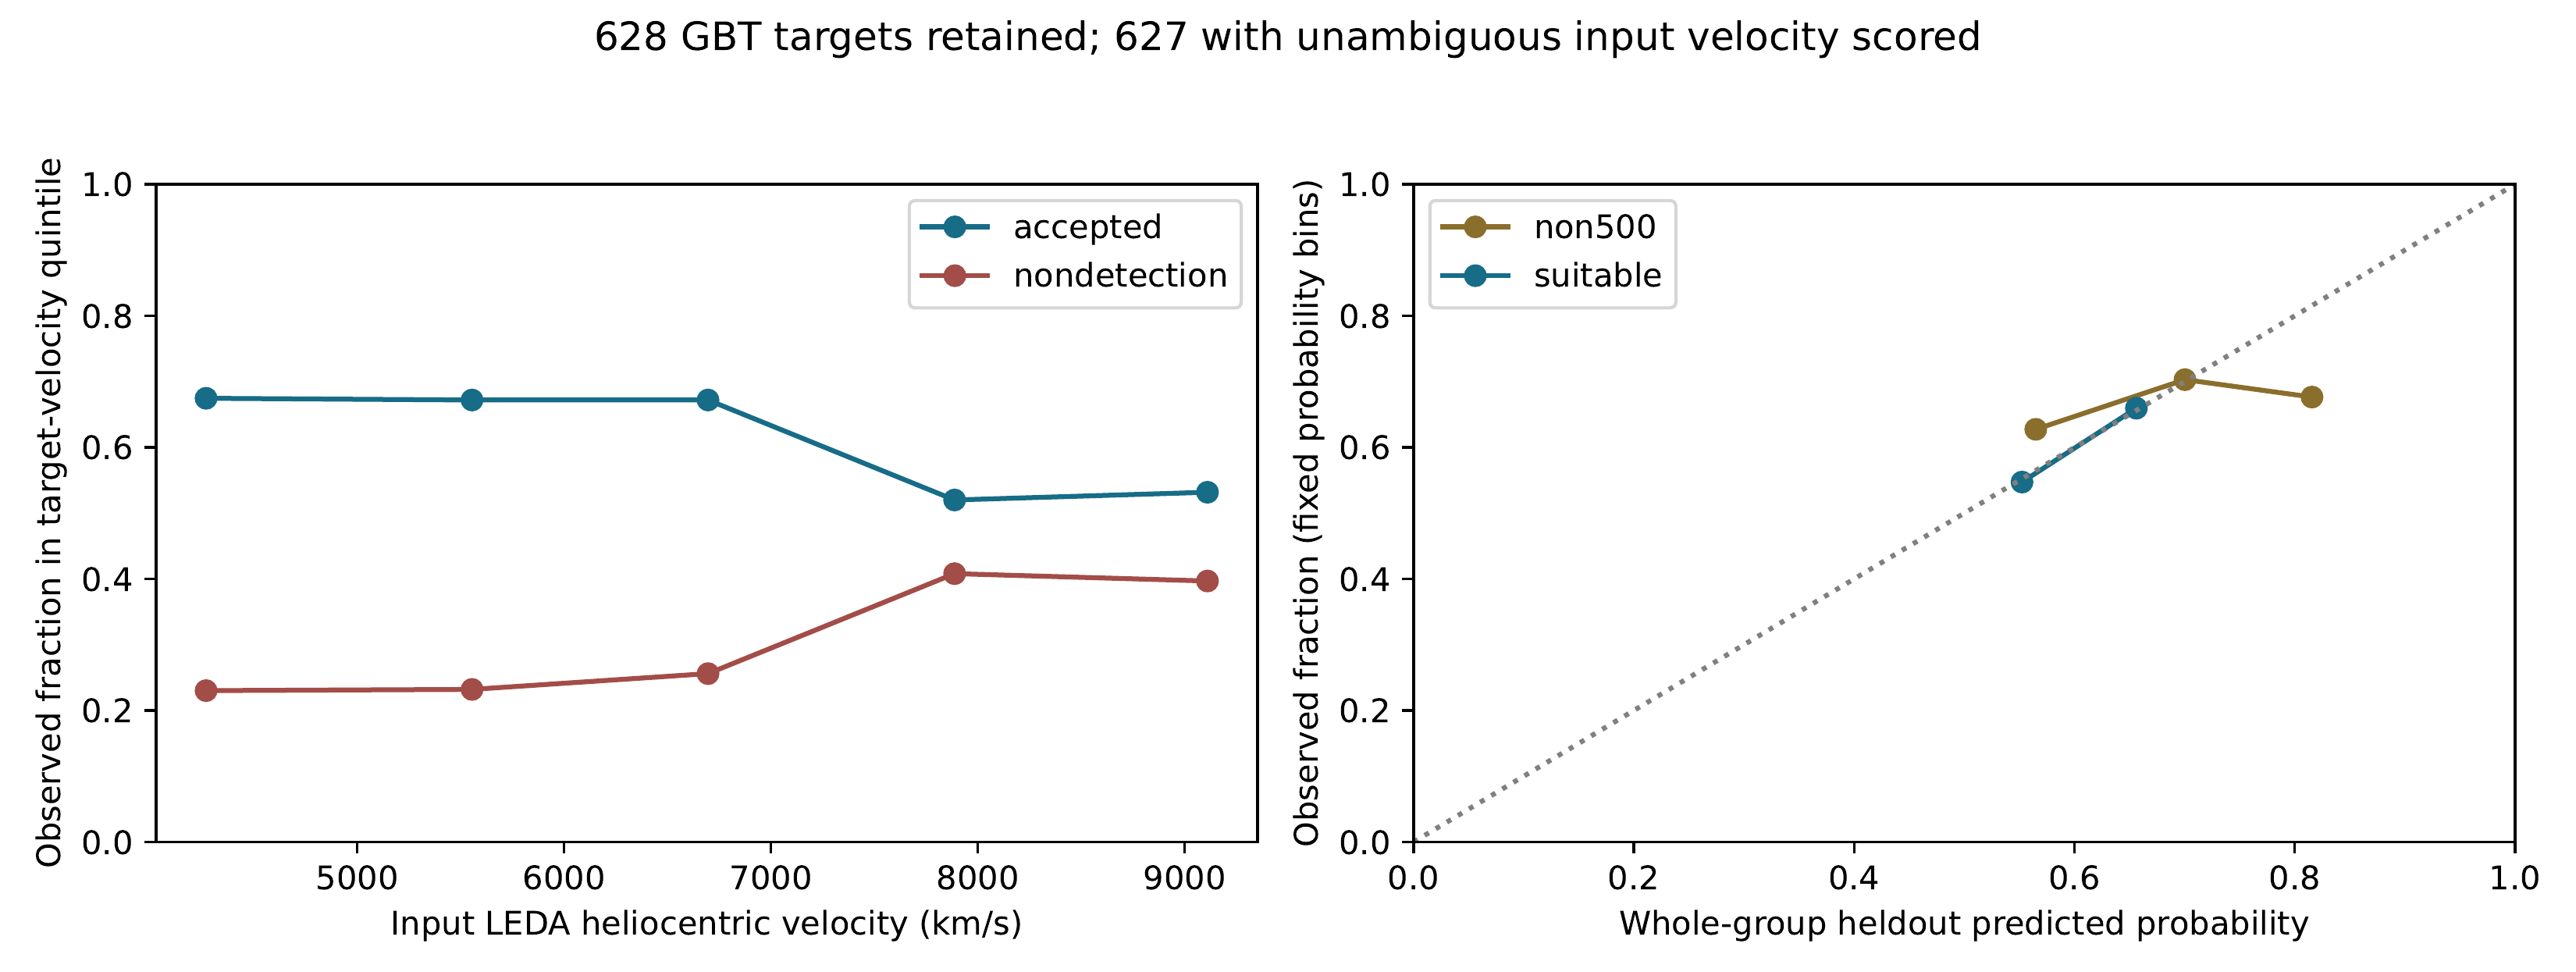
\includegraphics[width=\linewidth,height=.71\textheight,keepaspectratio]{figures/f069_external.png}
\caption{Outcome and velocity distributions in the retained hydrogen-line target cohort. Released distances, nondetections, and other quality outcomes remain distinct. These source counts and descriptive conditional fits do not supply a physical covariance or selected-parent null law.}
\label{fig:f069}
\end{figure}
\clearpage
\begin{figure}[p]
\centering
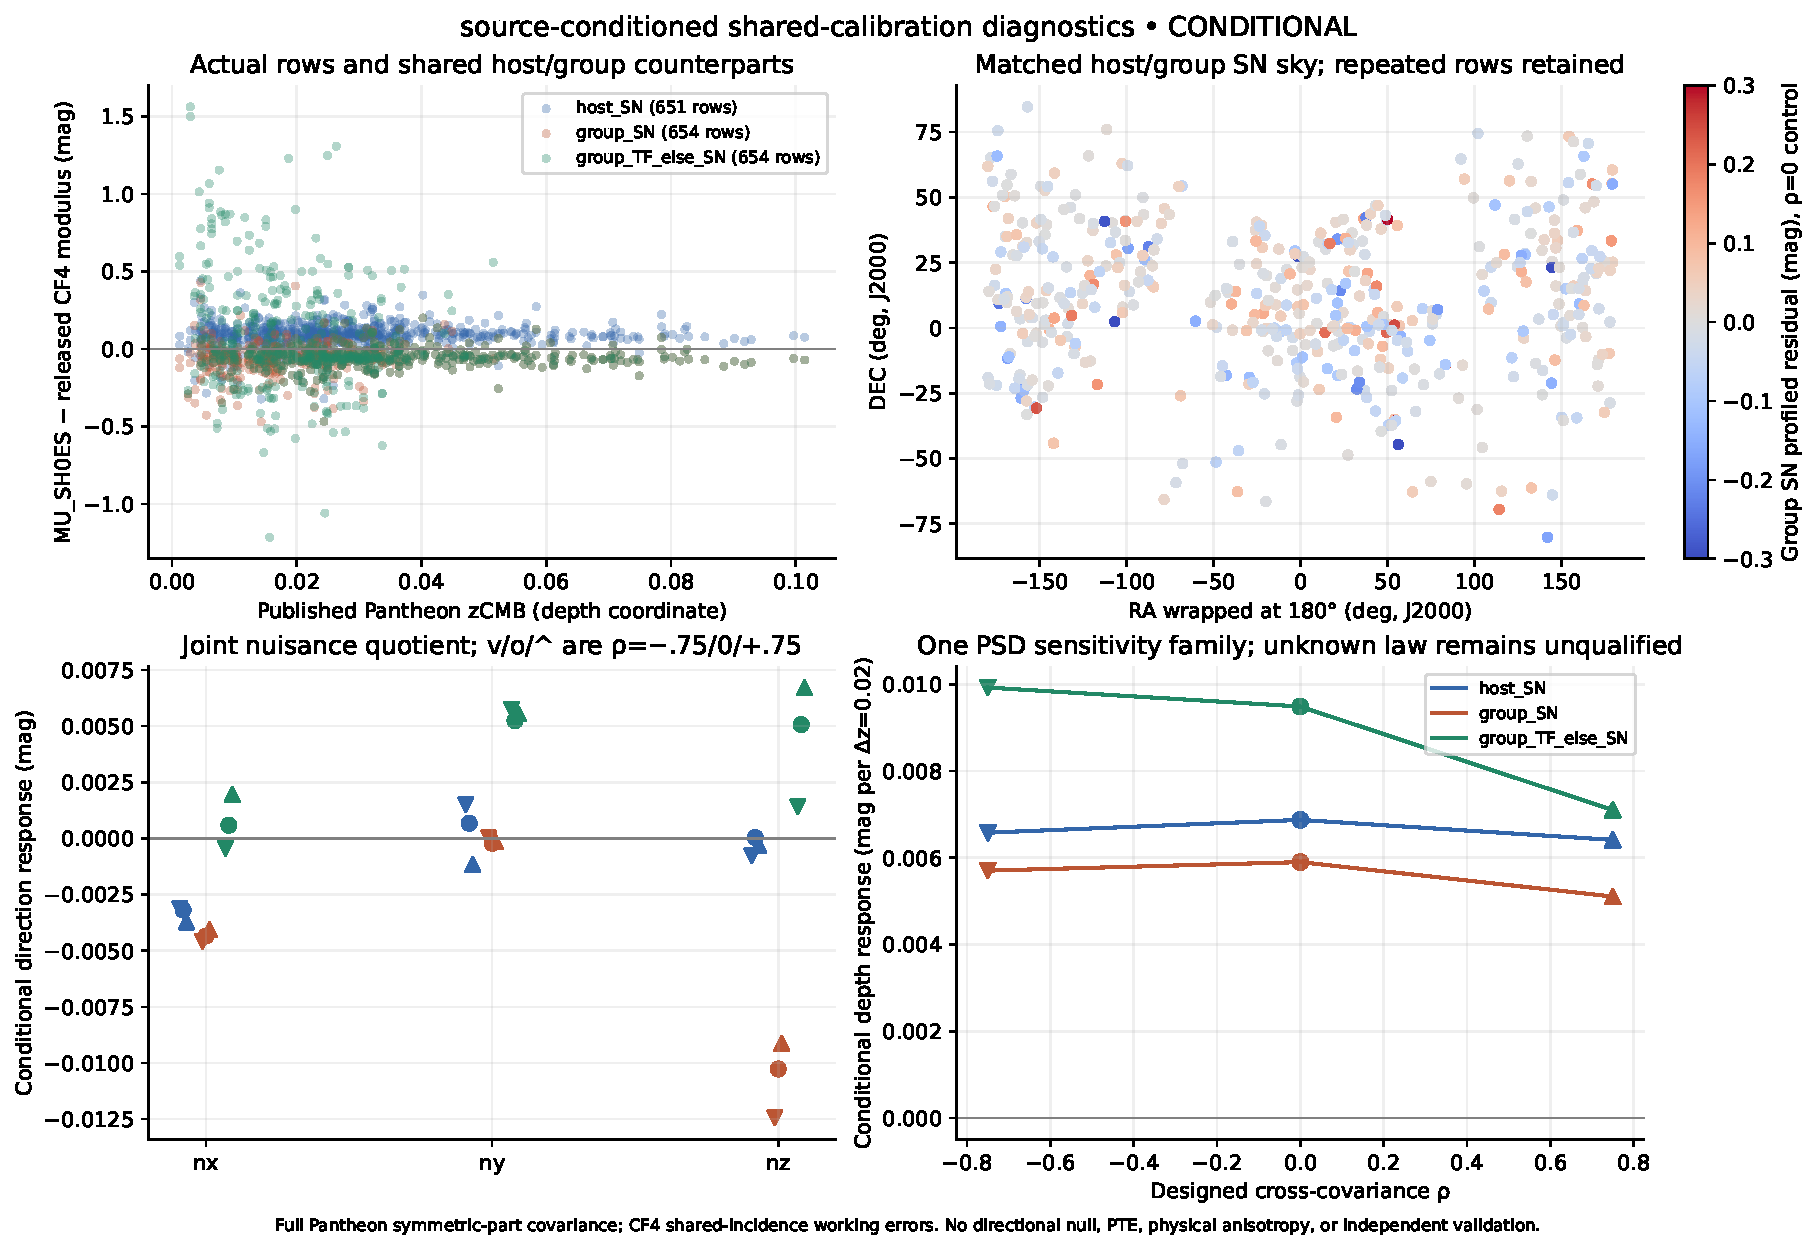
\includegraphics[width=\linewidth,height=.71\textheight,keepaspectratio]{figures/f070_external.pdf}
\caption{Pantheon+ and Cosmicflows comparisons on matched host and group sky positions. Repeated supernova rows and alternative host/group assignments are retained. Their differences are dependent source comparisons, not independent survey likelihood factors.}
\label{fig:f070}
\end{figure}
\clearpage
\begin{figure}[p]
\centering
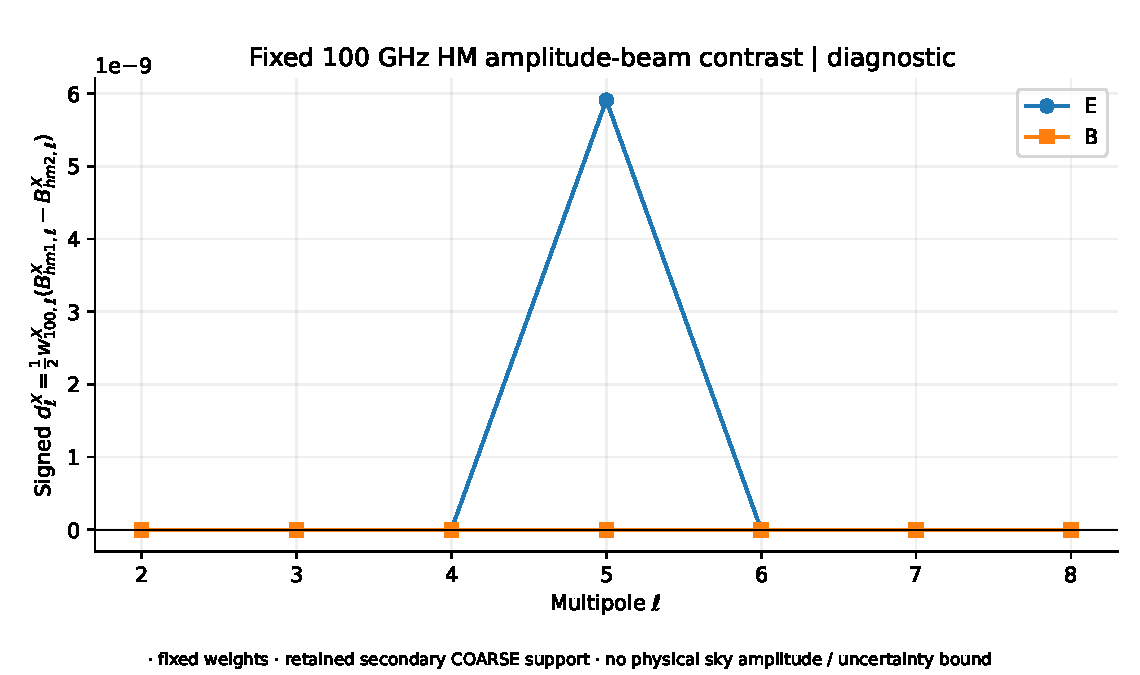
\includegraphics[width=\linewidth,height=.71\textheight,keepaspectratio]{figures/f071_external.pdf}
\caption{Fixed 100-GHz half-mission amplitude-beam contrast using retained coarse component weights. The displayed gains are properties of the declared finite operator. They are not measured sky contamination amplitudes or observational uncertainty bounds.}
\label{fig:f071}
\end{figure}
\clearpage
\begin{figure}[p]
\centering
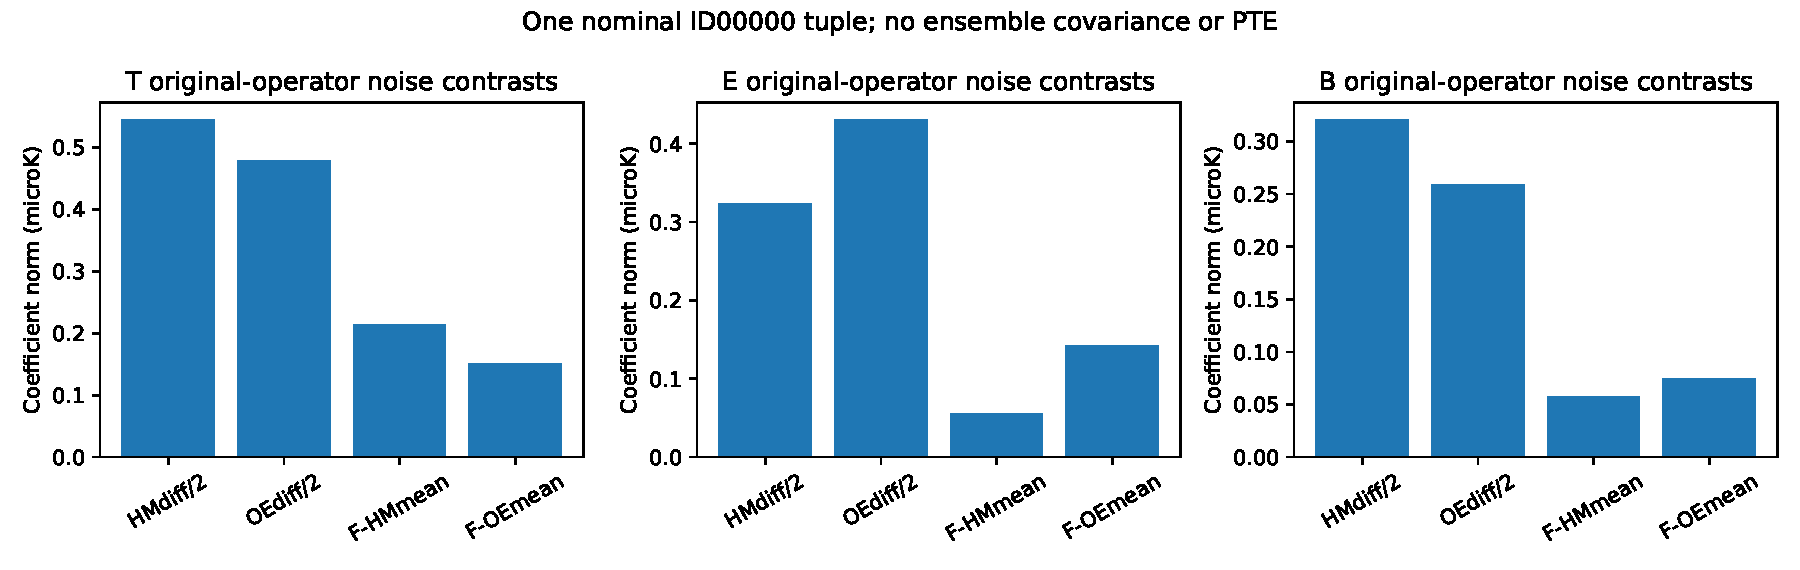
\includegraphics[width=\linewidth,height=.71\textheight,keepaspectratio]{figures/f072.pdf}
\caption{Finite split contrasts for one nominal signal/noise tuple on the stated support. A single tuple can expose a response difference but cannot estimate an ensemble covariance or a probability to exceed. Common sky components and split cross-noise remain relevant.}
\label{fig:f072}
\end{figure}
\clearpage
\begin{figure}[p]
\centering
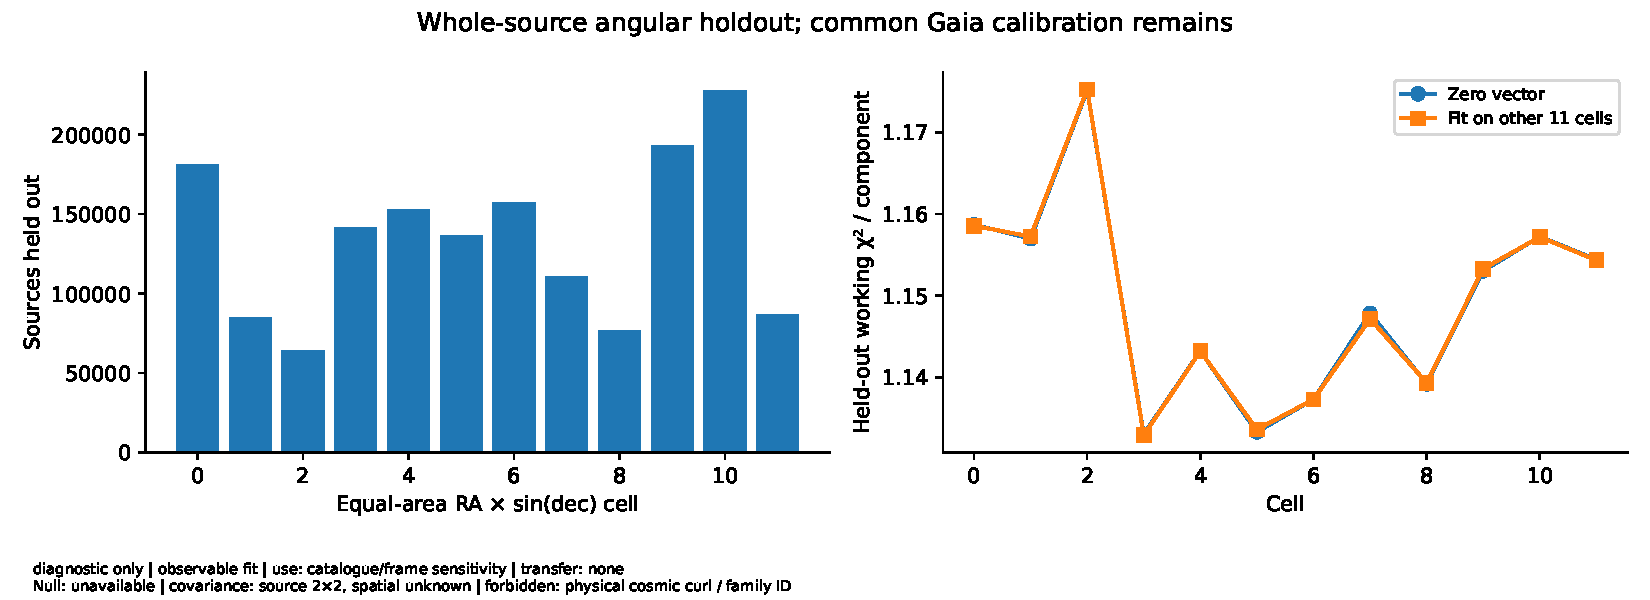
\includegraphics[width=\linewidth,height=.71\textheight,keepaspectratio]{figures/f073_external.pdf}
\caption{Whole-source angular holdout of the full Gaia frame-source sample. Held-out residual quadratics and retained counts probe spatial variation under a working covariance. Common Gaia calibration survives this split, so it does not create an independent physical validation sample.}
\label{fig:f073}
\end{figure}
\clearpage
\begin{figure}[p]
\centering
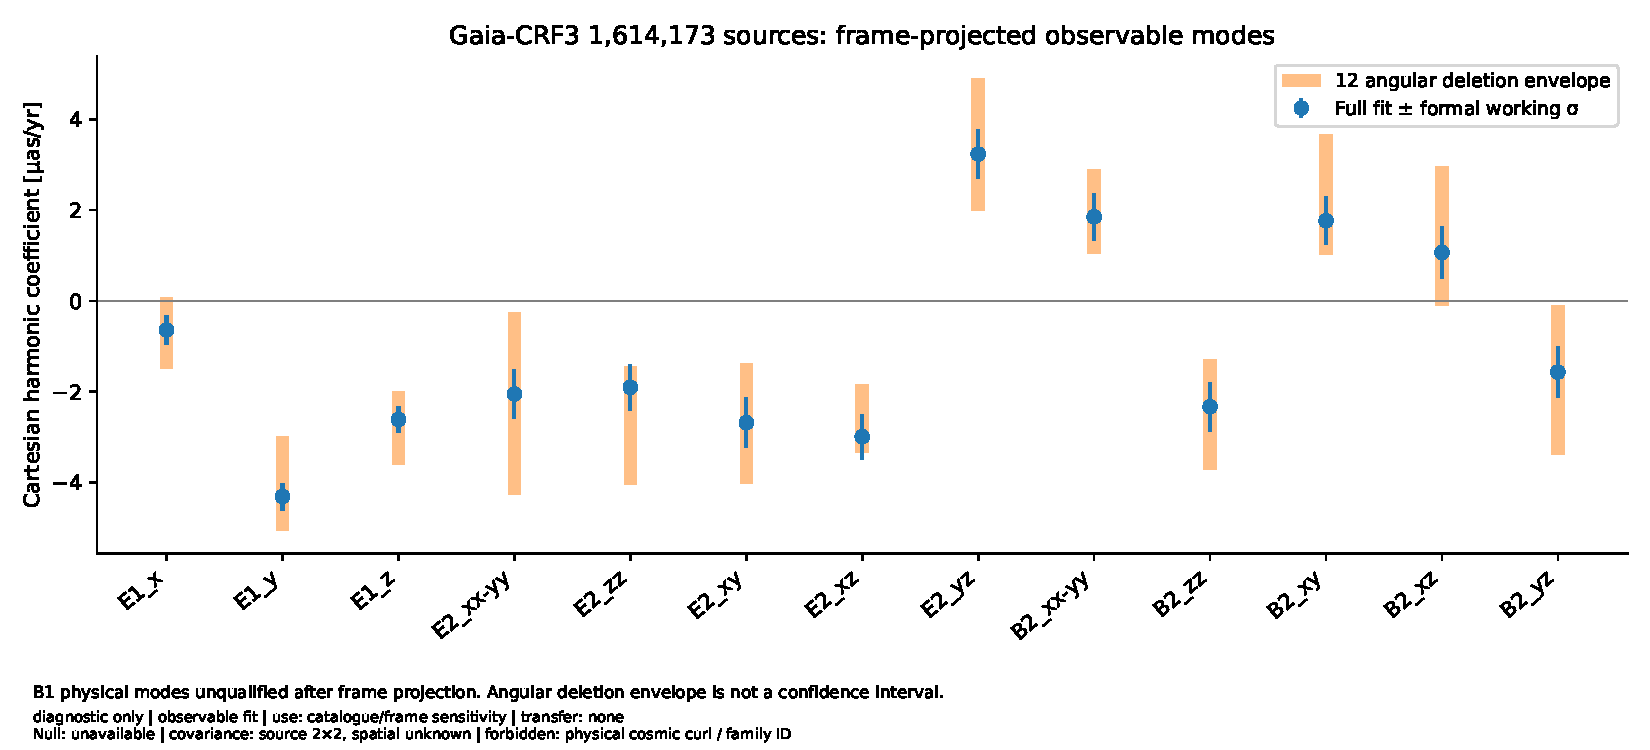
\includegraphics[width=\linewidth,height=.71\textheight,keepaspectratio]{figures/f074_external.pdf}
\caption{Frame-projected vector-spherical-harmonic coefficients in the full Gaia-CRF3 catalogue, with angular-deletion sensitivity. Formal errors use reported source blocks. The retained vector and STF modes are observable fields, not directly measured matter acceleration, shear, or vorticity.}
\label{fig:f074}
\end{figure}
\clearpage
\begin{figure}[p]
\centering
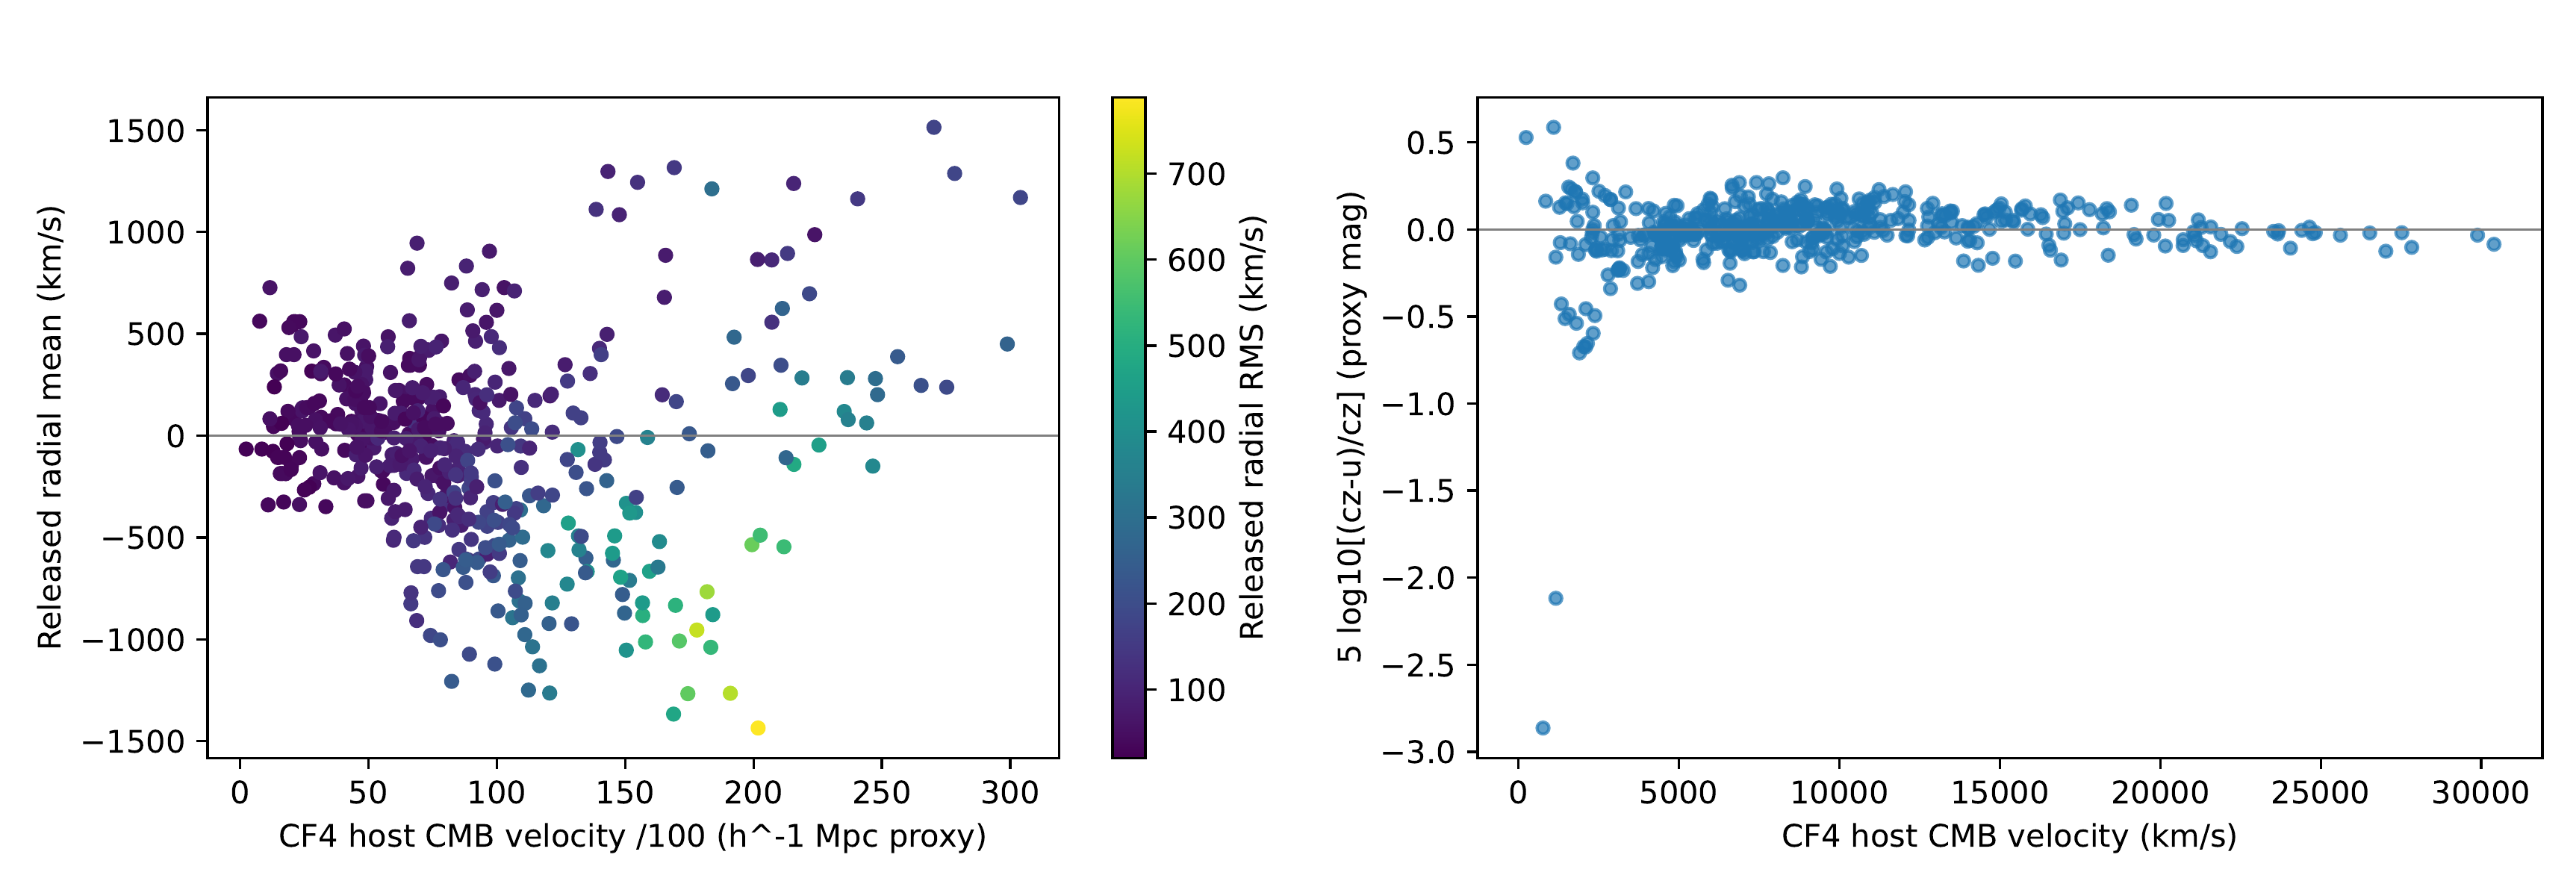
\includegraphics[width=\linewidth,height=.71\textheight,keepaspectratio]{figures/f075_external.png}
\caption{Corrected Cosmicflows reconstruction evaluated at matched hosts. Radial values and magnitude shifts are dependent source and algebraic proxy diagnostics. The lookup is not a physical luminosity-distance correction and has no supplied joint covariance with the host distances.}
\label{fig:f075}
\end{figure}
\clearpage
\begin{figure}[p]
\centering
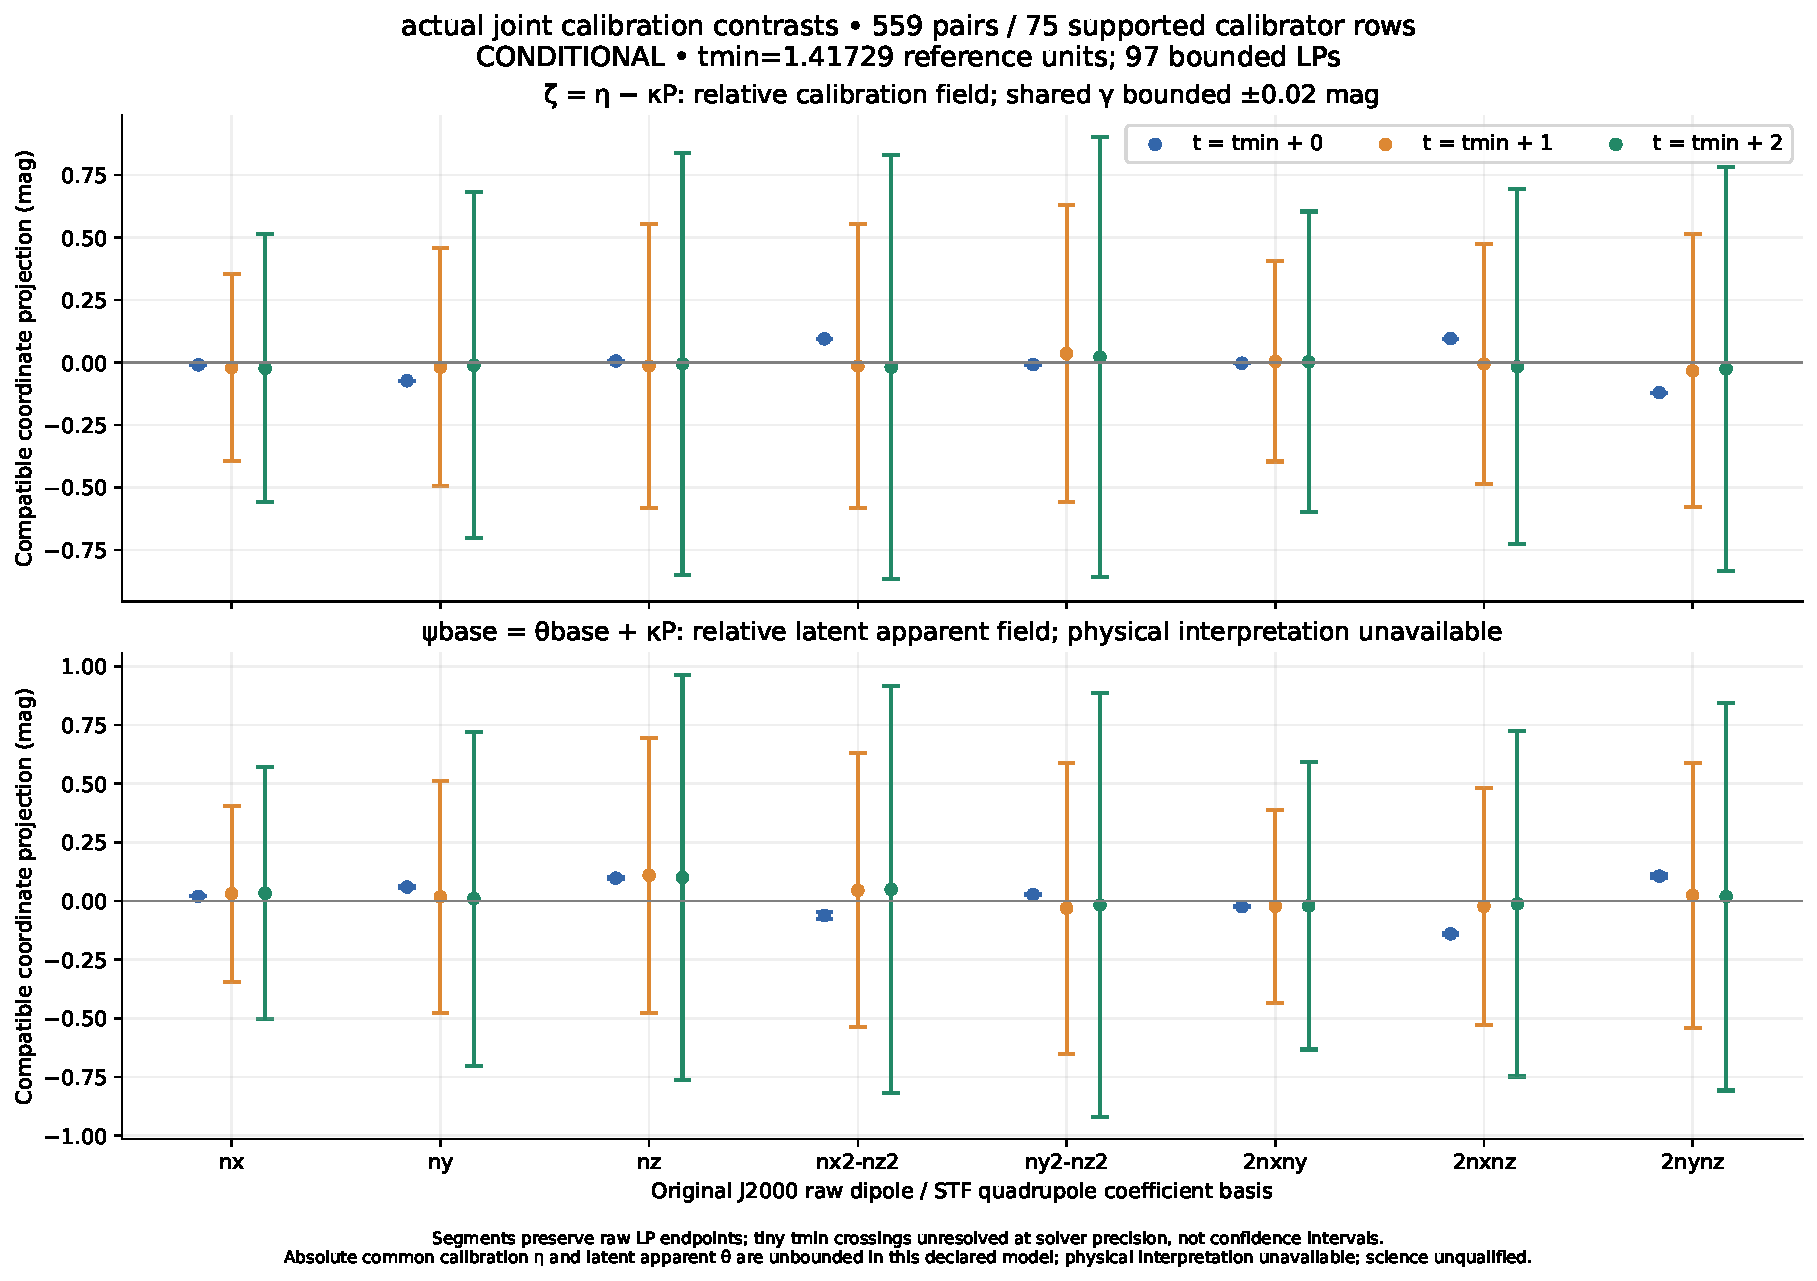
\includegraphics[width=\linewidth,height=.71\textheight,keepaspectratio]{figures/f076_external.pdf}
\caption{Joint calibration contrasts on shared hosts and groups. Identified combinations have bounded reference-coordinate projections, while common absolute calibration and other gauge directions remain unbounded. The minimum reference radius is dimensionless and is not a noise quantile or physical confidence bound.}
\label{fig:f076}
\end{figure}
\clearpage
\begin{figure}[p]
\centering
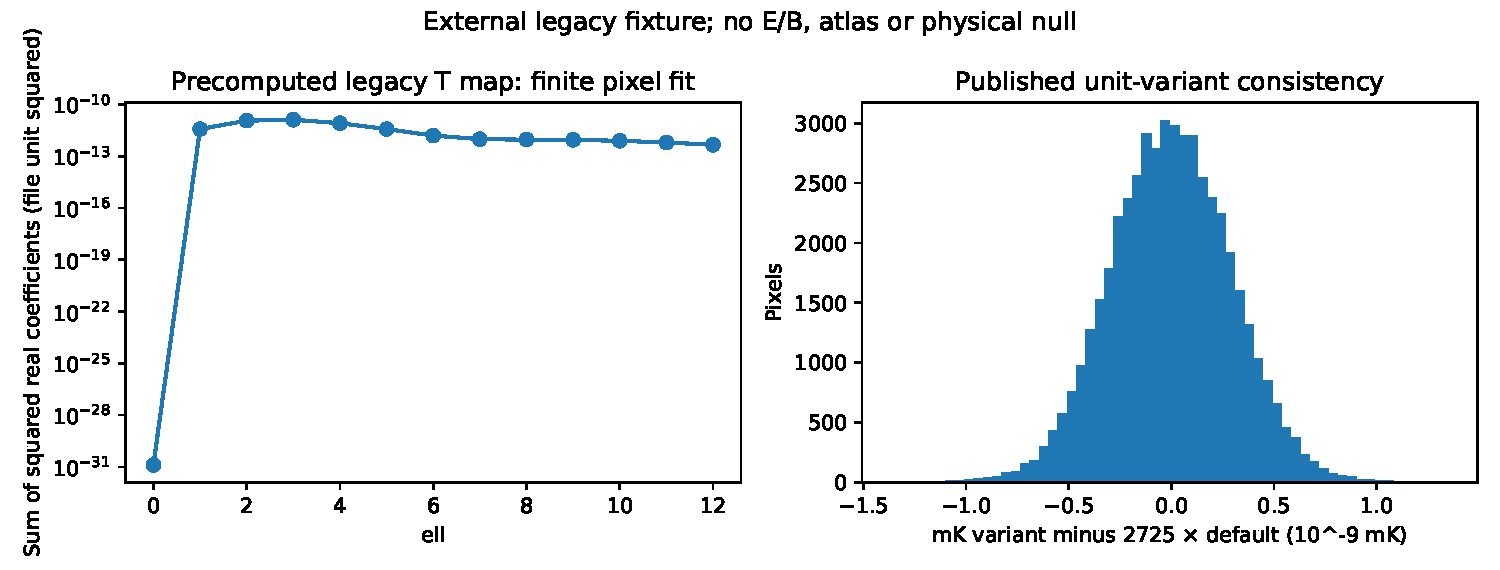
\includegraphics[width=\linewidth,height=.71\textheight,keepaspectratio]{figures/f077.pdf}
\caption{Finite harmonic representation of a precomputed external temperature-only template and its unit variants. Polarization is absent, not zero; the absolute sky frame and physical atlas eligibility are unqualified. This external template is not a native solver result.}
\label{fig:f077}
\end{figure}
\clearpage
\begin{figure}[p]
\centering
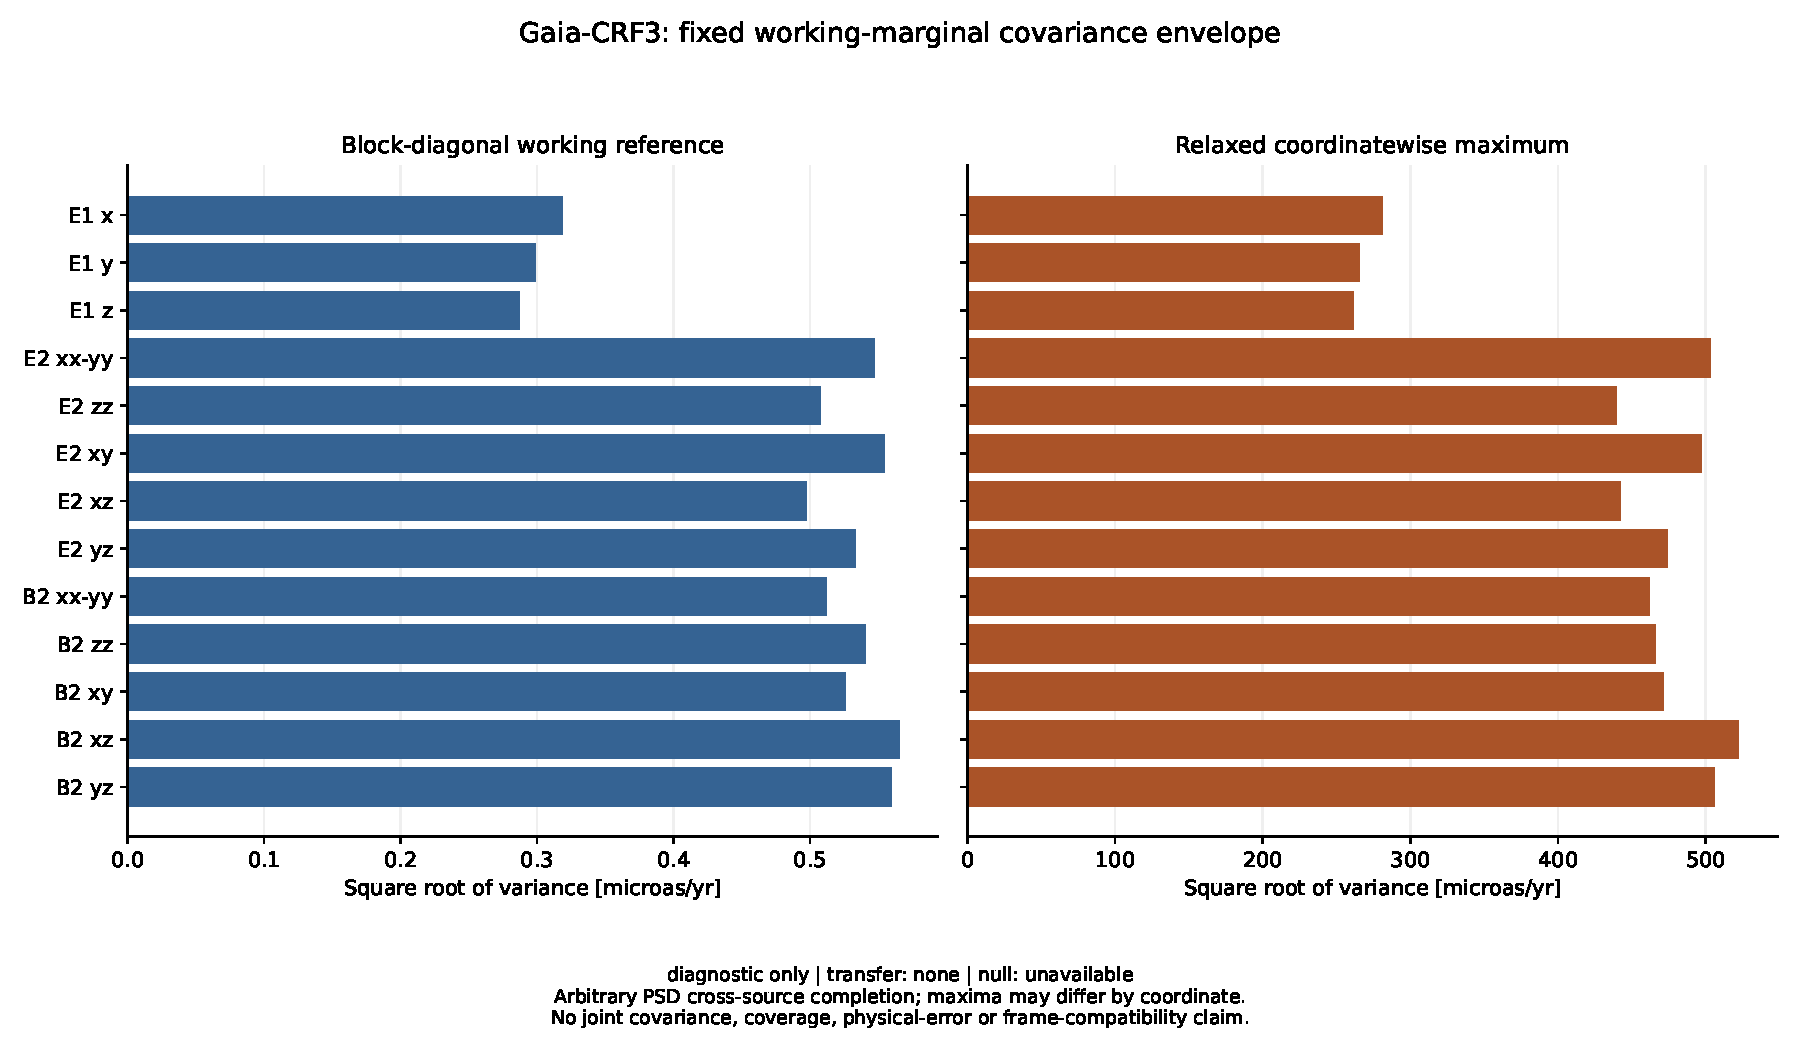
\includegraphics[width=\linewidth,height=.71\textheight,keepaspectratio]{figures/f078_external.pdf}
\caption{Coordinatewise covariance envelopes for the Gaia observable fit with working marginals held fixed. Arbitrary positive-semidefinite dependence can enlarge individual error scales. Different extrema are not jointly attainable by assumption, and the plot is not a measured spatial covariance or one matrix upper bound.}
\label{fig:f078}
\end{figure}
\clearpage
\begin{figure}[p]
\centering
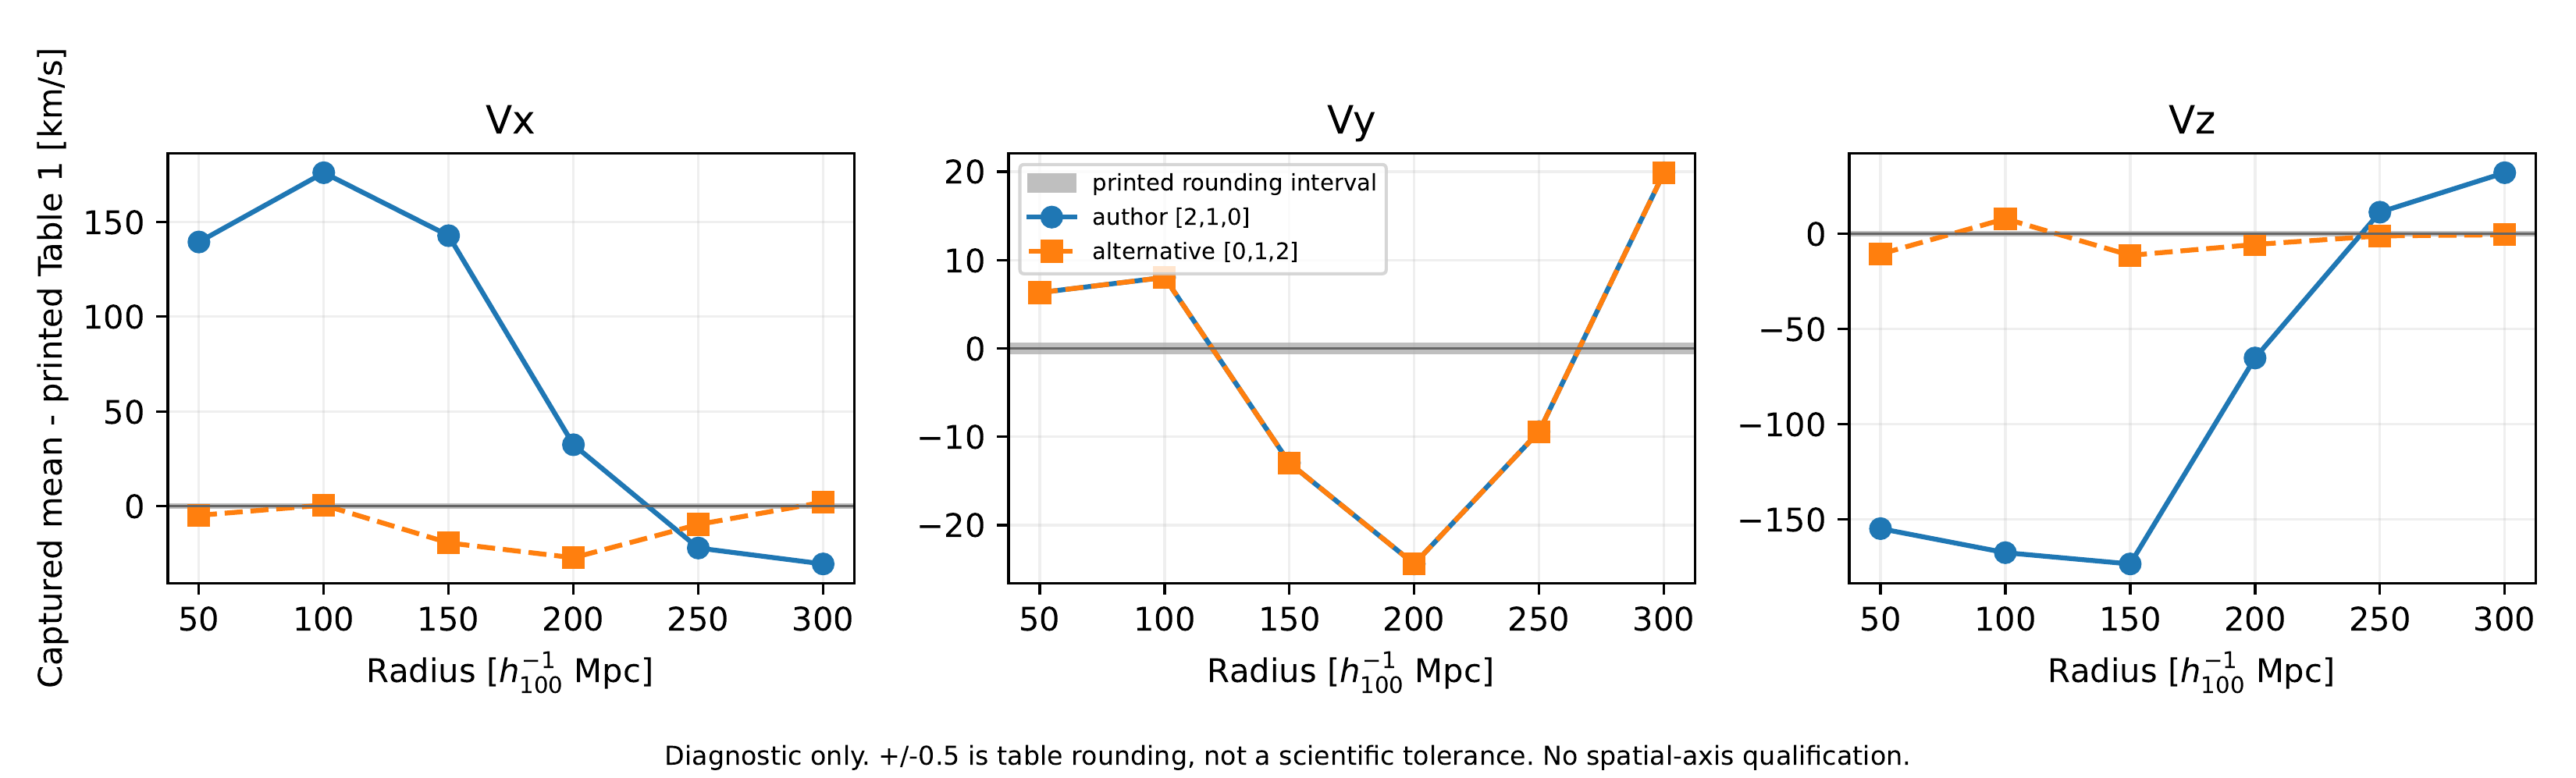
\includegraphics[width=\linewidth,height=.71\textheight,keepaspectratio]{figures/f079_external.png}
\caption{Comparison of a captured grouped-flow source with its printed summary under the specified coordinate-order alternatives. The source discrepancy remains unresolved. Neither coordinate substitution nor a close subset comparison establishes full source parity.}
\label{fig:f079}
\end{figure}
\clearpage
\begin{figure}[p]
\centering
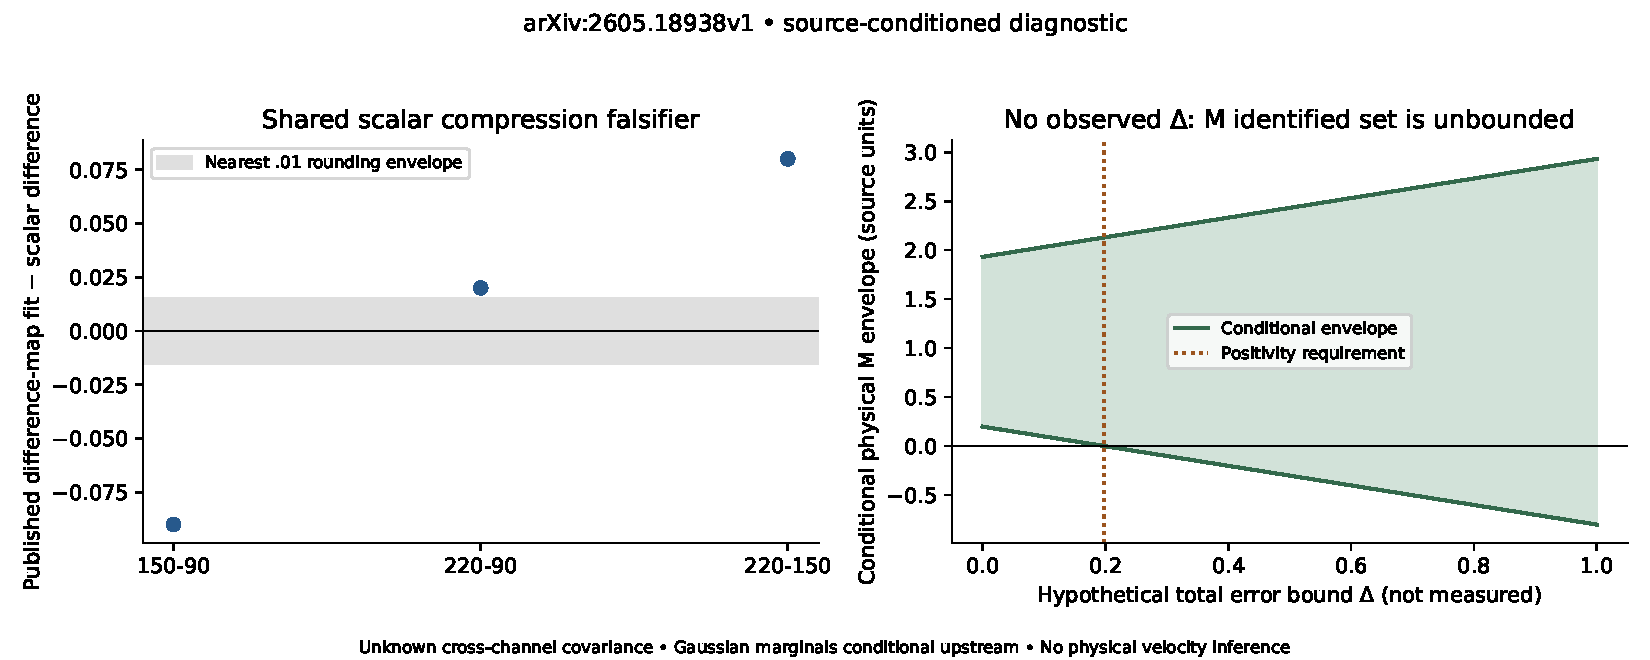
\includegraphics[width=\linewidth,height=.71\textheight,keepaspectratio]{figures/f080_external.pdf}
\caption{Source-conditioned moving-lens amplitude contrasts and a falsifier of shared scalar compression. The displayed intervals assume the stated marginal laws and rounding allowance. No observed differential filter or spectral-error bound is supplied; the physical amplitude therefore remains unbounded.}
\label{fig:f080}
\end{figure}
\clearpage
\begin{figure}[p]
\centering
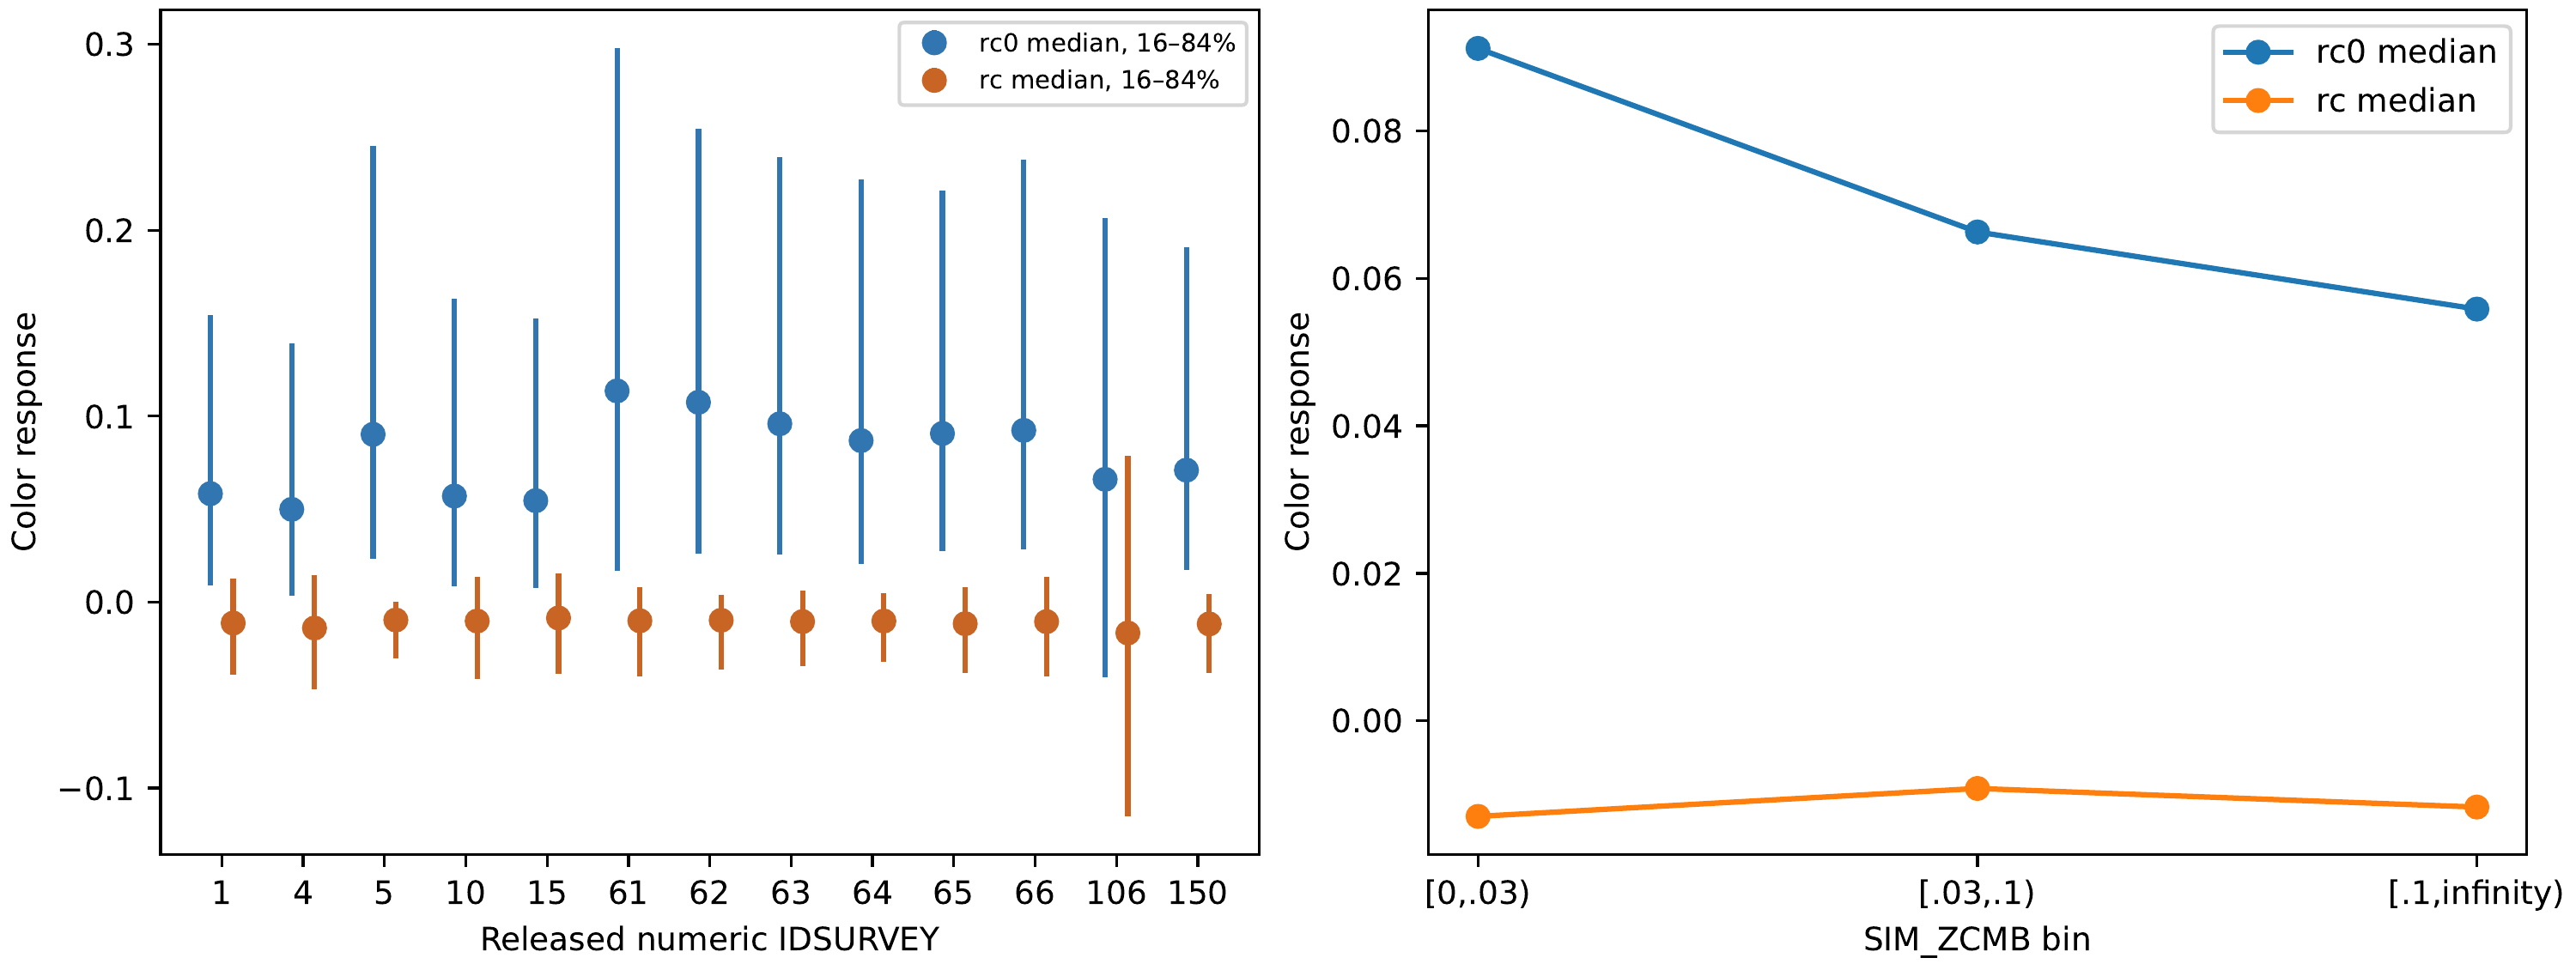
\includegraphics[width=\linewidth,height=.71\textheight,keepaspectratio]{figures/f081_external.png}
\caption{Colour response in released selected supernova simulations, before and after the stated dust-predictor adjustment. The rows and source model define this simulation diagnostic. It is not an empirical total reboost response or calibrated observed-survey correction.}
\label{fig:f081}
\end{figure}
\clearpage
\begin{figure}[p]
\centering
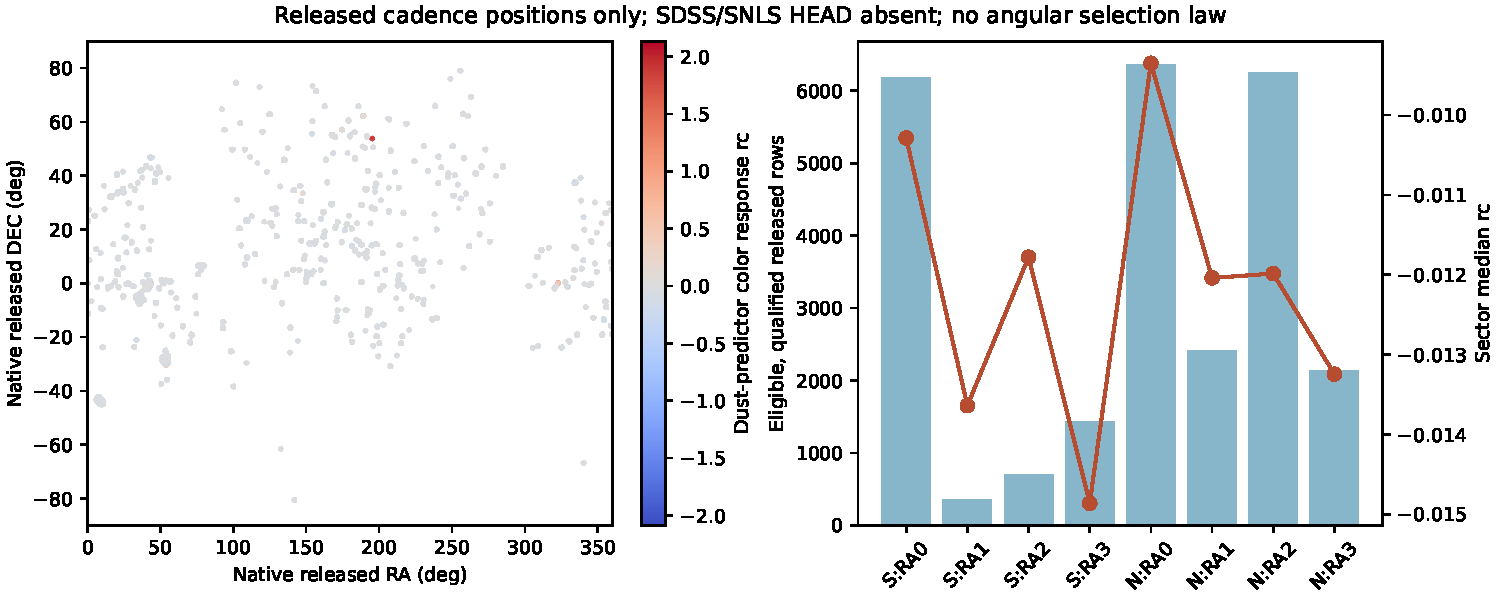
\includegraphics[width=\linewidth,height=.71\textheight,keepaspectratio]{figures/f082.pdf}
\caption{Released directions and sky variation of the selected supernova simulation response. Qualified angular coordinates are retained, with missing directions excluded explicitly. Directional patterns in these simulations do not establish physical sky anisotropy.}
\label{fig:f082}
\end{figure}
\clearpage
\begin{figure}[p]
\centering
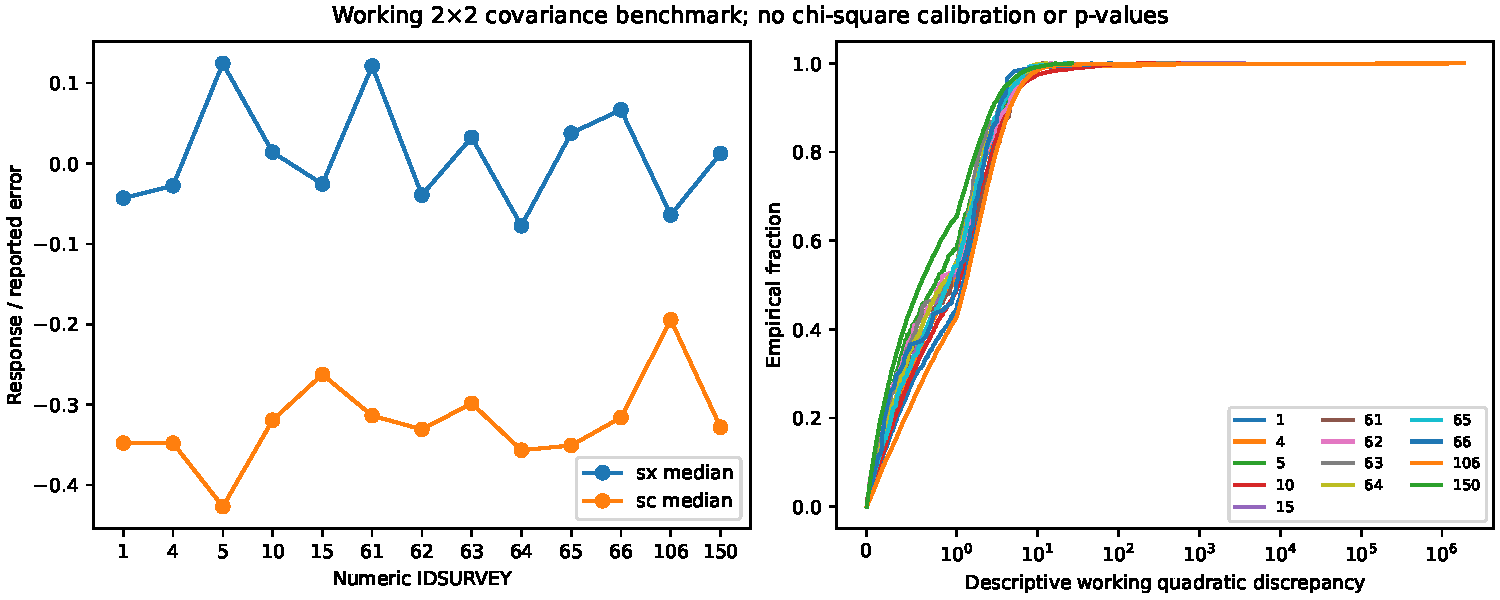
\includegraphics[width=\linewidth,height=.71\textheight,keepaspectratio]{figures/f083.pdf}
\caption{Working two-coordinate covariance benchmark for released supernova simulation responses. The displayed standardized responses and empirical fractions use their source-specific errors. No chi-square calibration, physical probability, or new observed-supernova likelihood is assigned.}
\label{fig:f083}
\end{figure}
\clearpage
\begin{figure}[p]
\centering
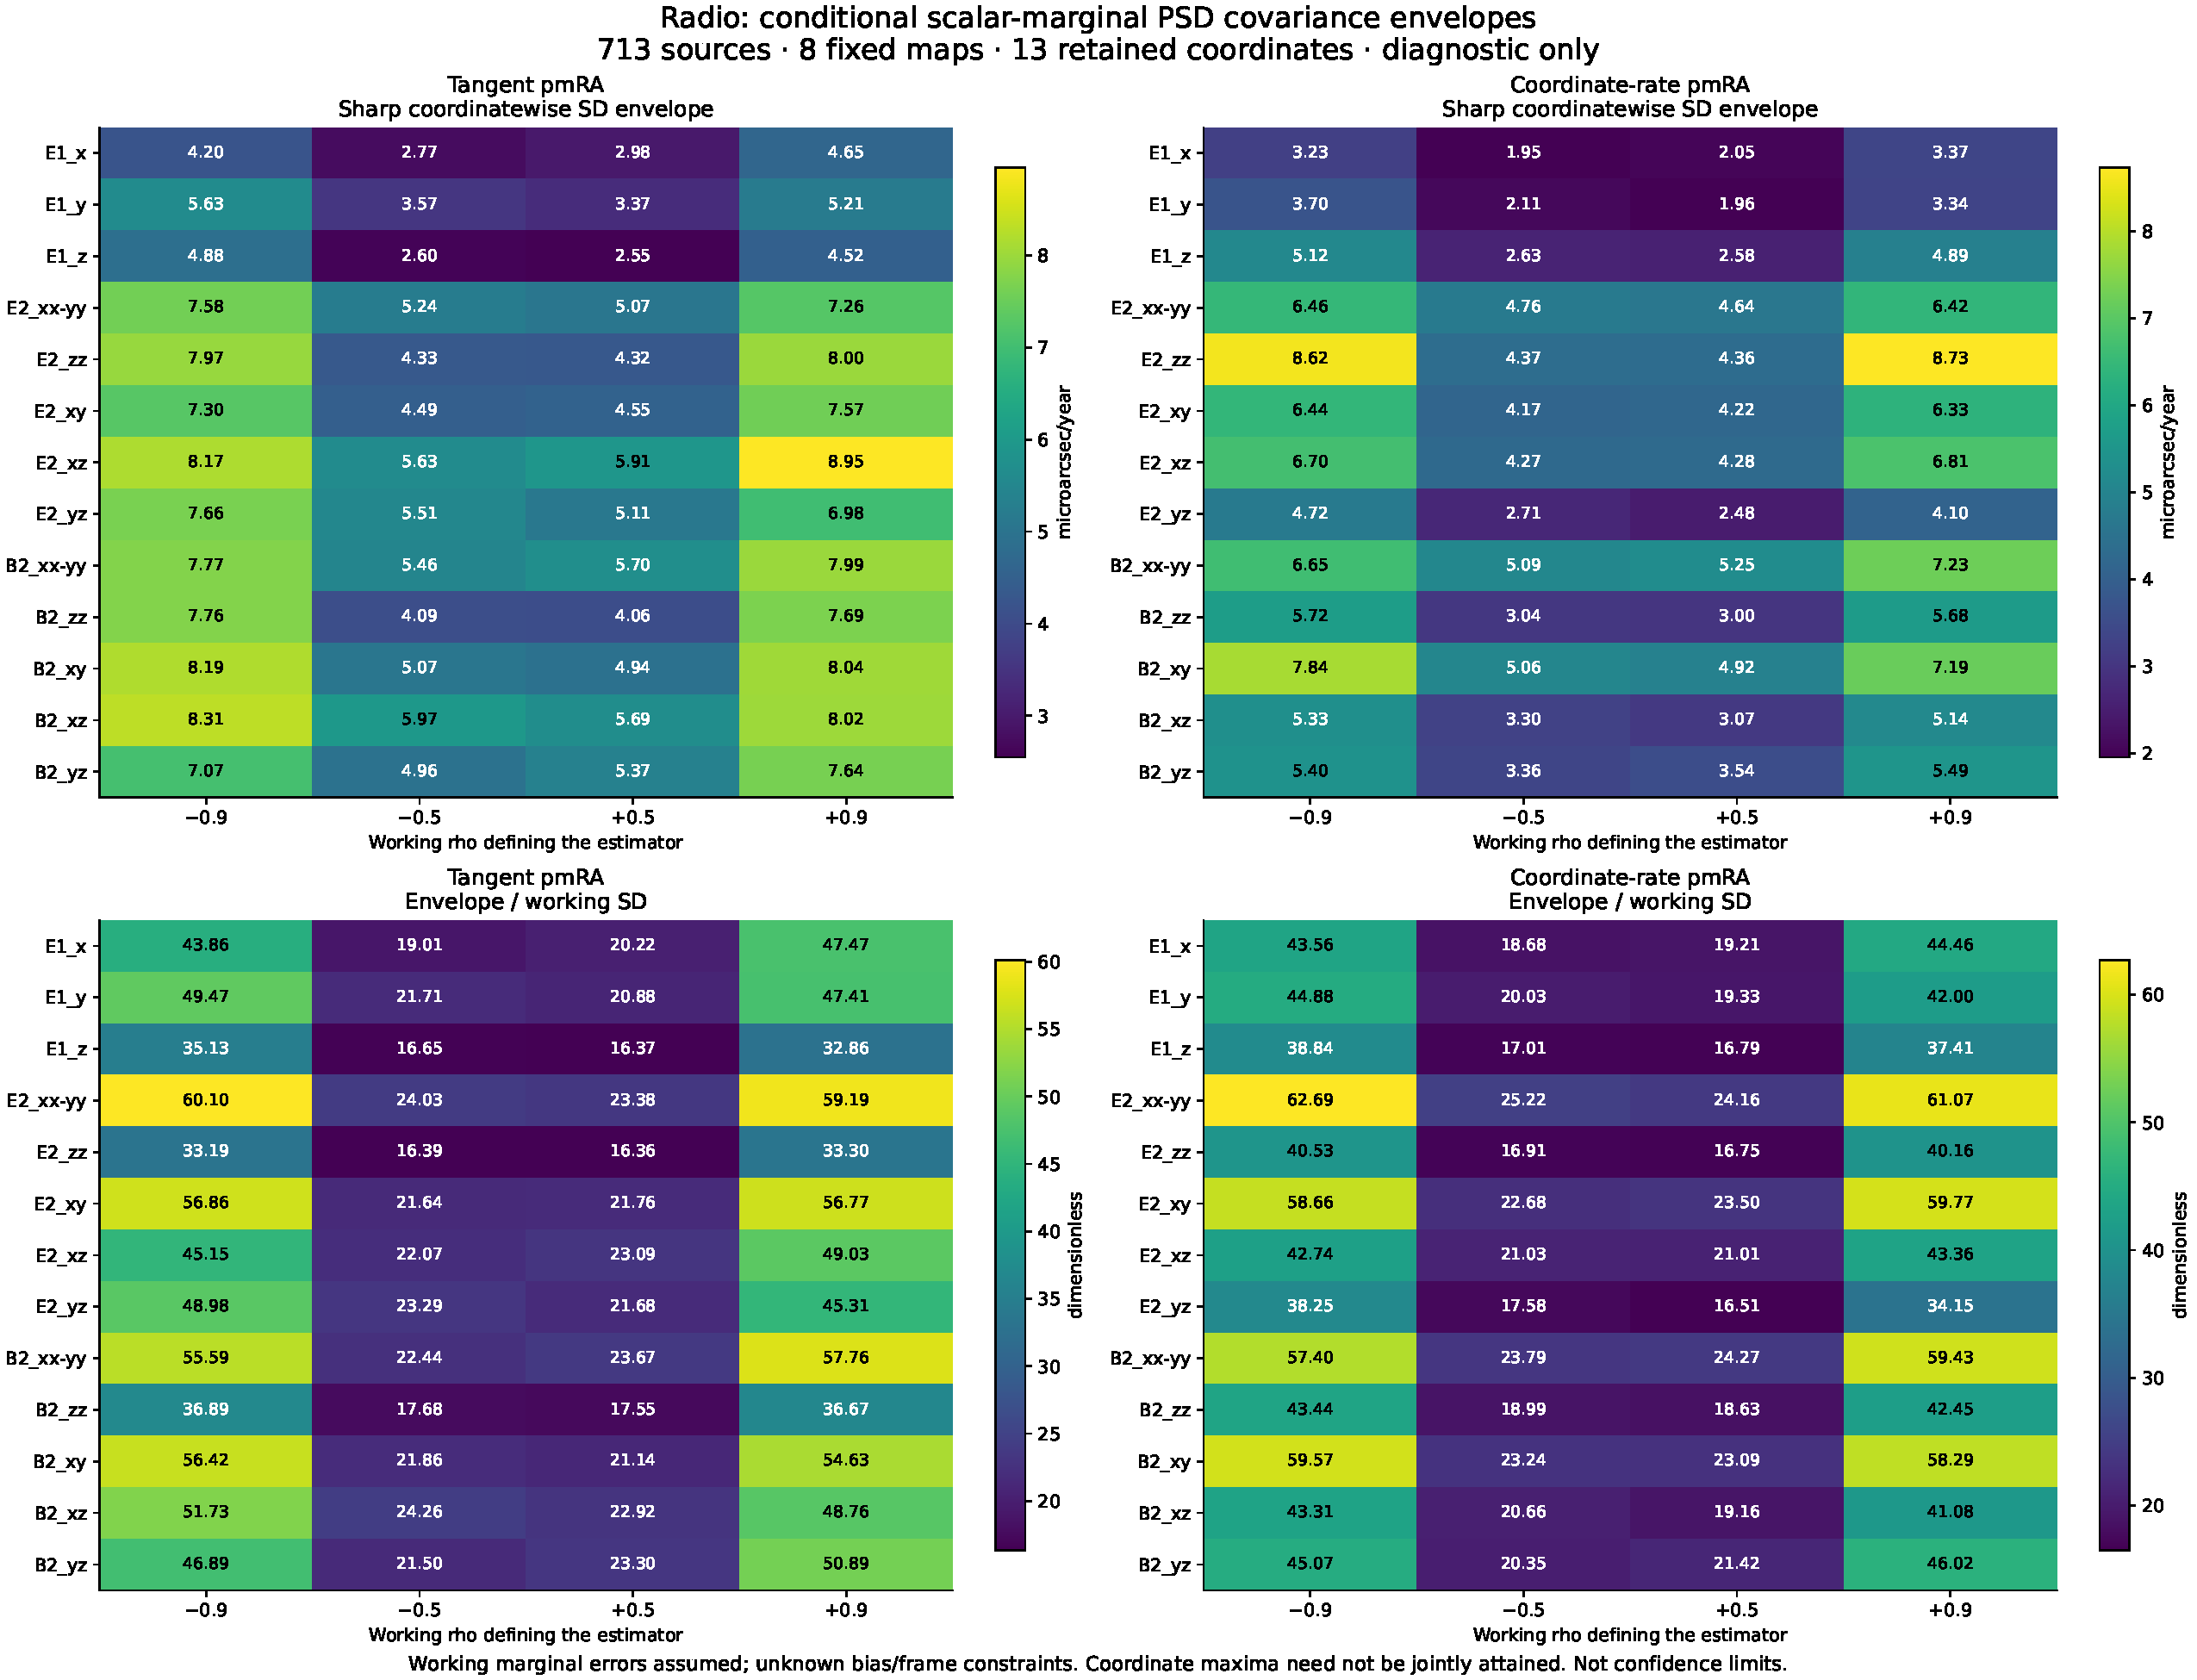
\includegraphics[width=\linewidth,height=.71\textheight,keepaspectratio]{figures/f084_external.pdf}
\caption{Radio proper-motion coordinate envelopes under fixed scalar marginals and stated correlation scenarios. The retained coordinate convention matters. These are separate sharp coordinate bounds, not a jointly attained covariance matrix or a calibrated optical--radio physical comparison.}
\label{fig:f084}
\end{figure}
\clearpage
\begin{figure}[p]
\centering
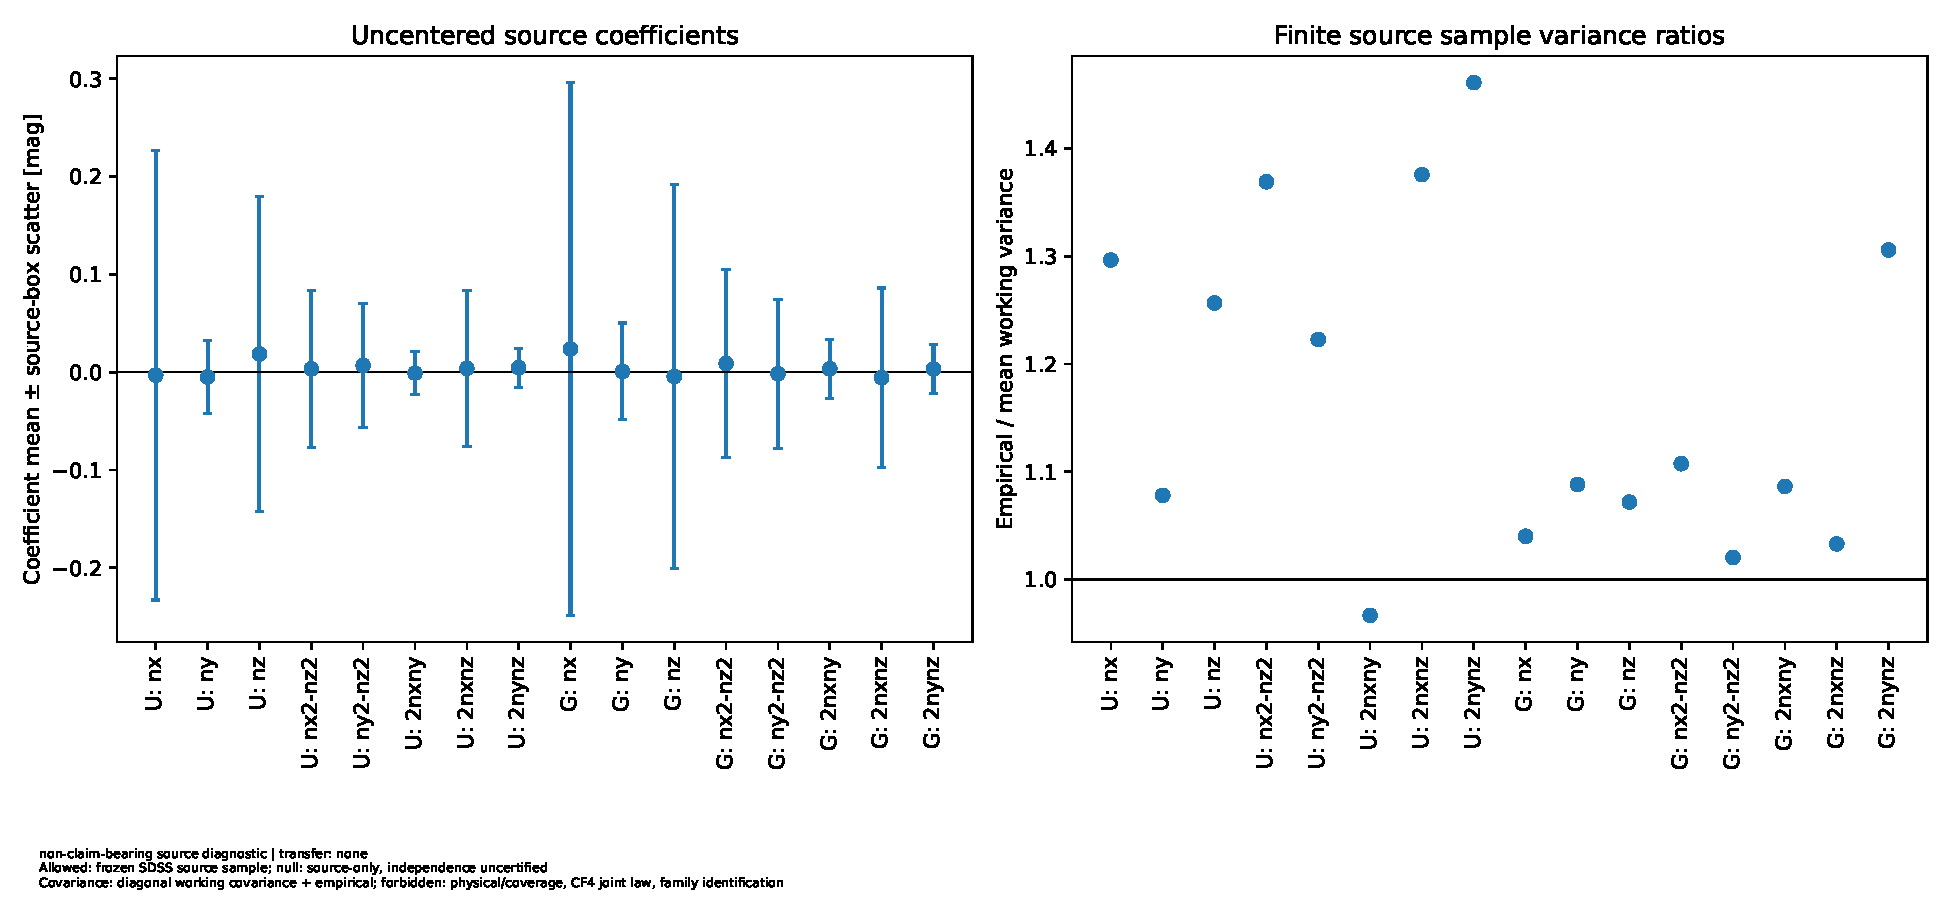
\includegraphics[width=\linewidth,height=.71\textheight,keepaspectratio]{figures/f085_external.pdf}
\caption{Uncentred coefficients and variance ratios from retained error-only SDSS source realizations. True source peculiar velocity is removed in this experiment. The finite sample diagnoses the stated error law and does not supply a physical velocity or selection null.}
\label{fig:f085}
\end{figure}
\clearpage
\begin{figure}[p]
\centering
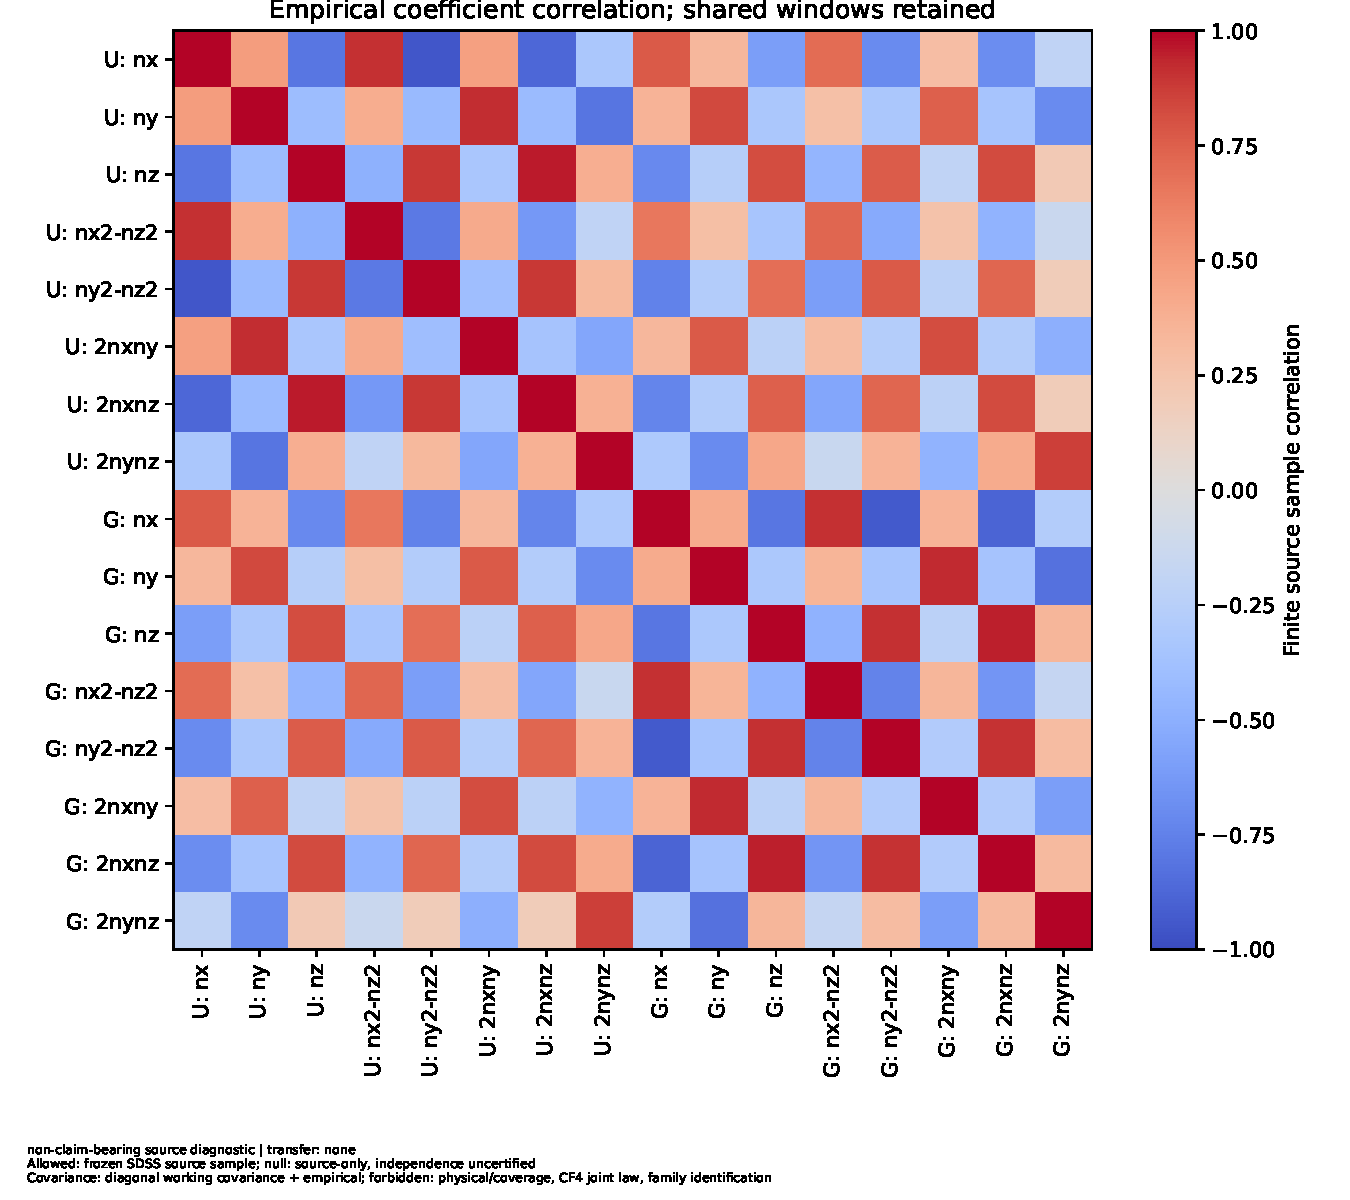
\includegraphics[width=\linewidth,height=.71\textheight,keepaspectratio]{figures/f086_external.pdf}
\caption{Empirical coefficient correlations in the same error-only source realizations. Shared angular windows remain coupled. The finite correlation matrix is descriptive and does not establish independence of the source boxes or a full physical survey covariance.}
\label{fig:f086}
\end{figure}
\clearpage
\begin{figure}[p]
\centering
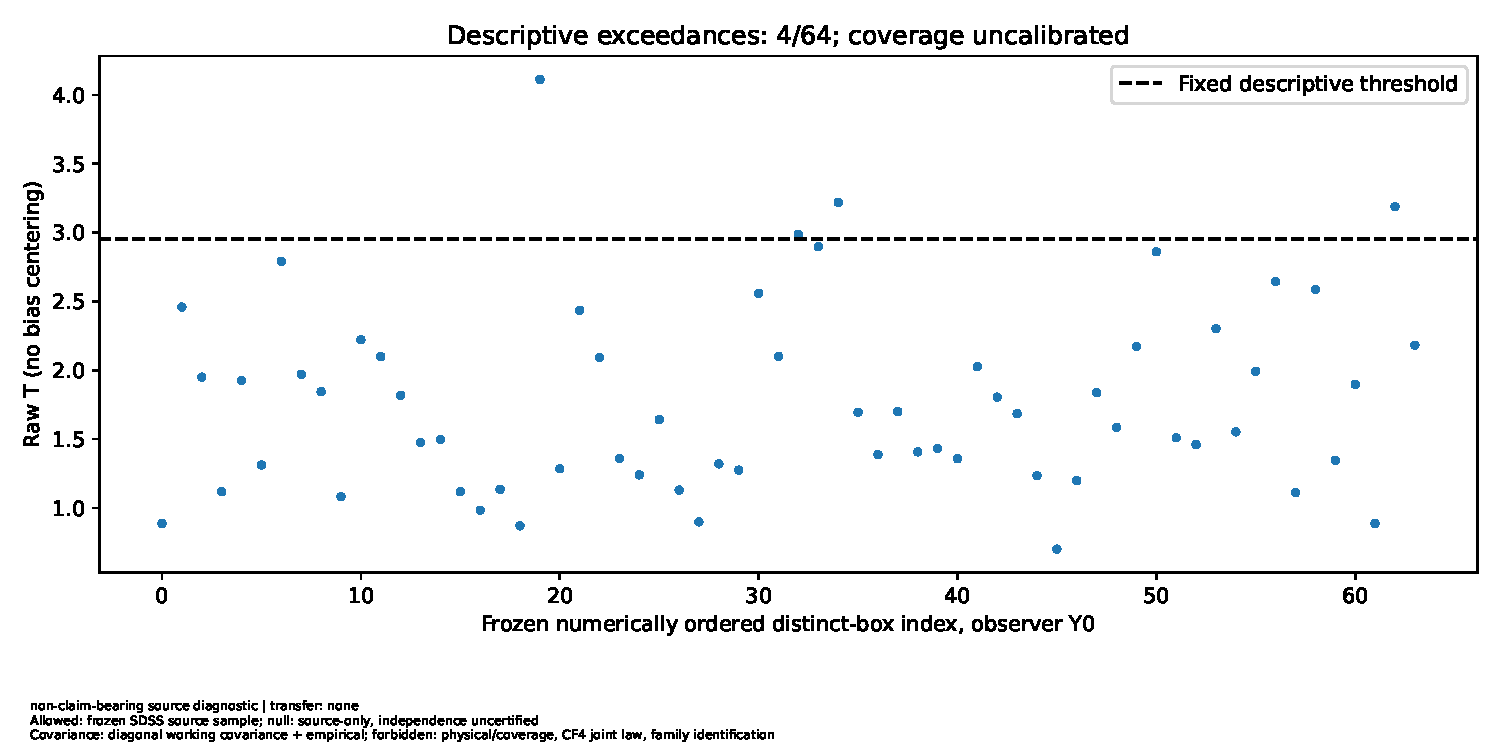
\includegraphics[width=\linewidth,height=.71\textheight,keepaspectratio]{figures/f087_external.pdf}
\caption{Raw descriptive quadratics for the retained error-only source realizations. The fixed threshold is not a calibrated physical acceptance region. Exceedance counts and uncentred bias are retained without converting them into survey coverage.}
\label{fig:f087}
\end{figure}
\clearpage
\begin{figure}[p]
\centering
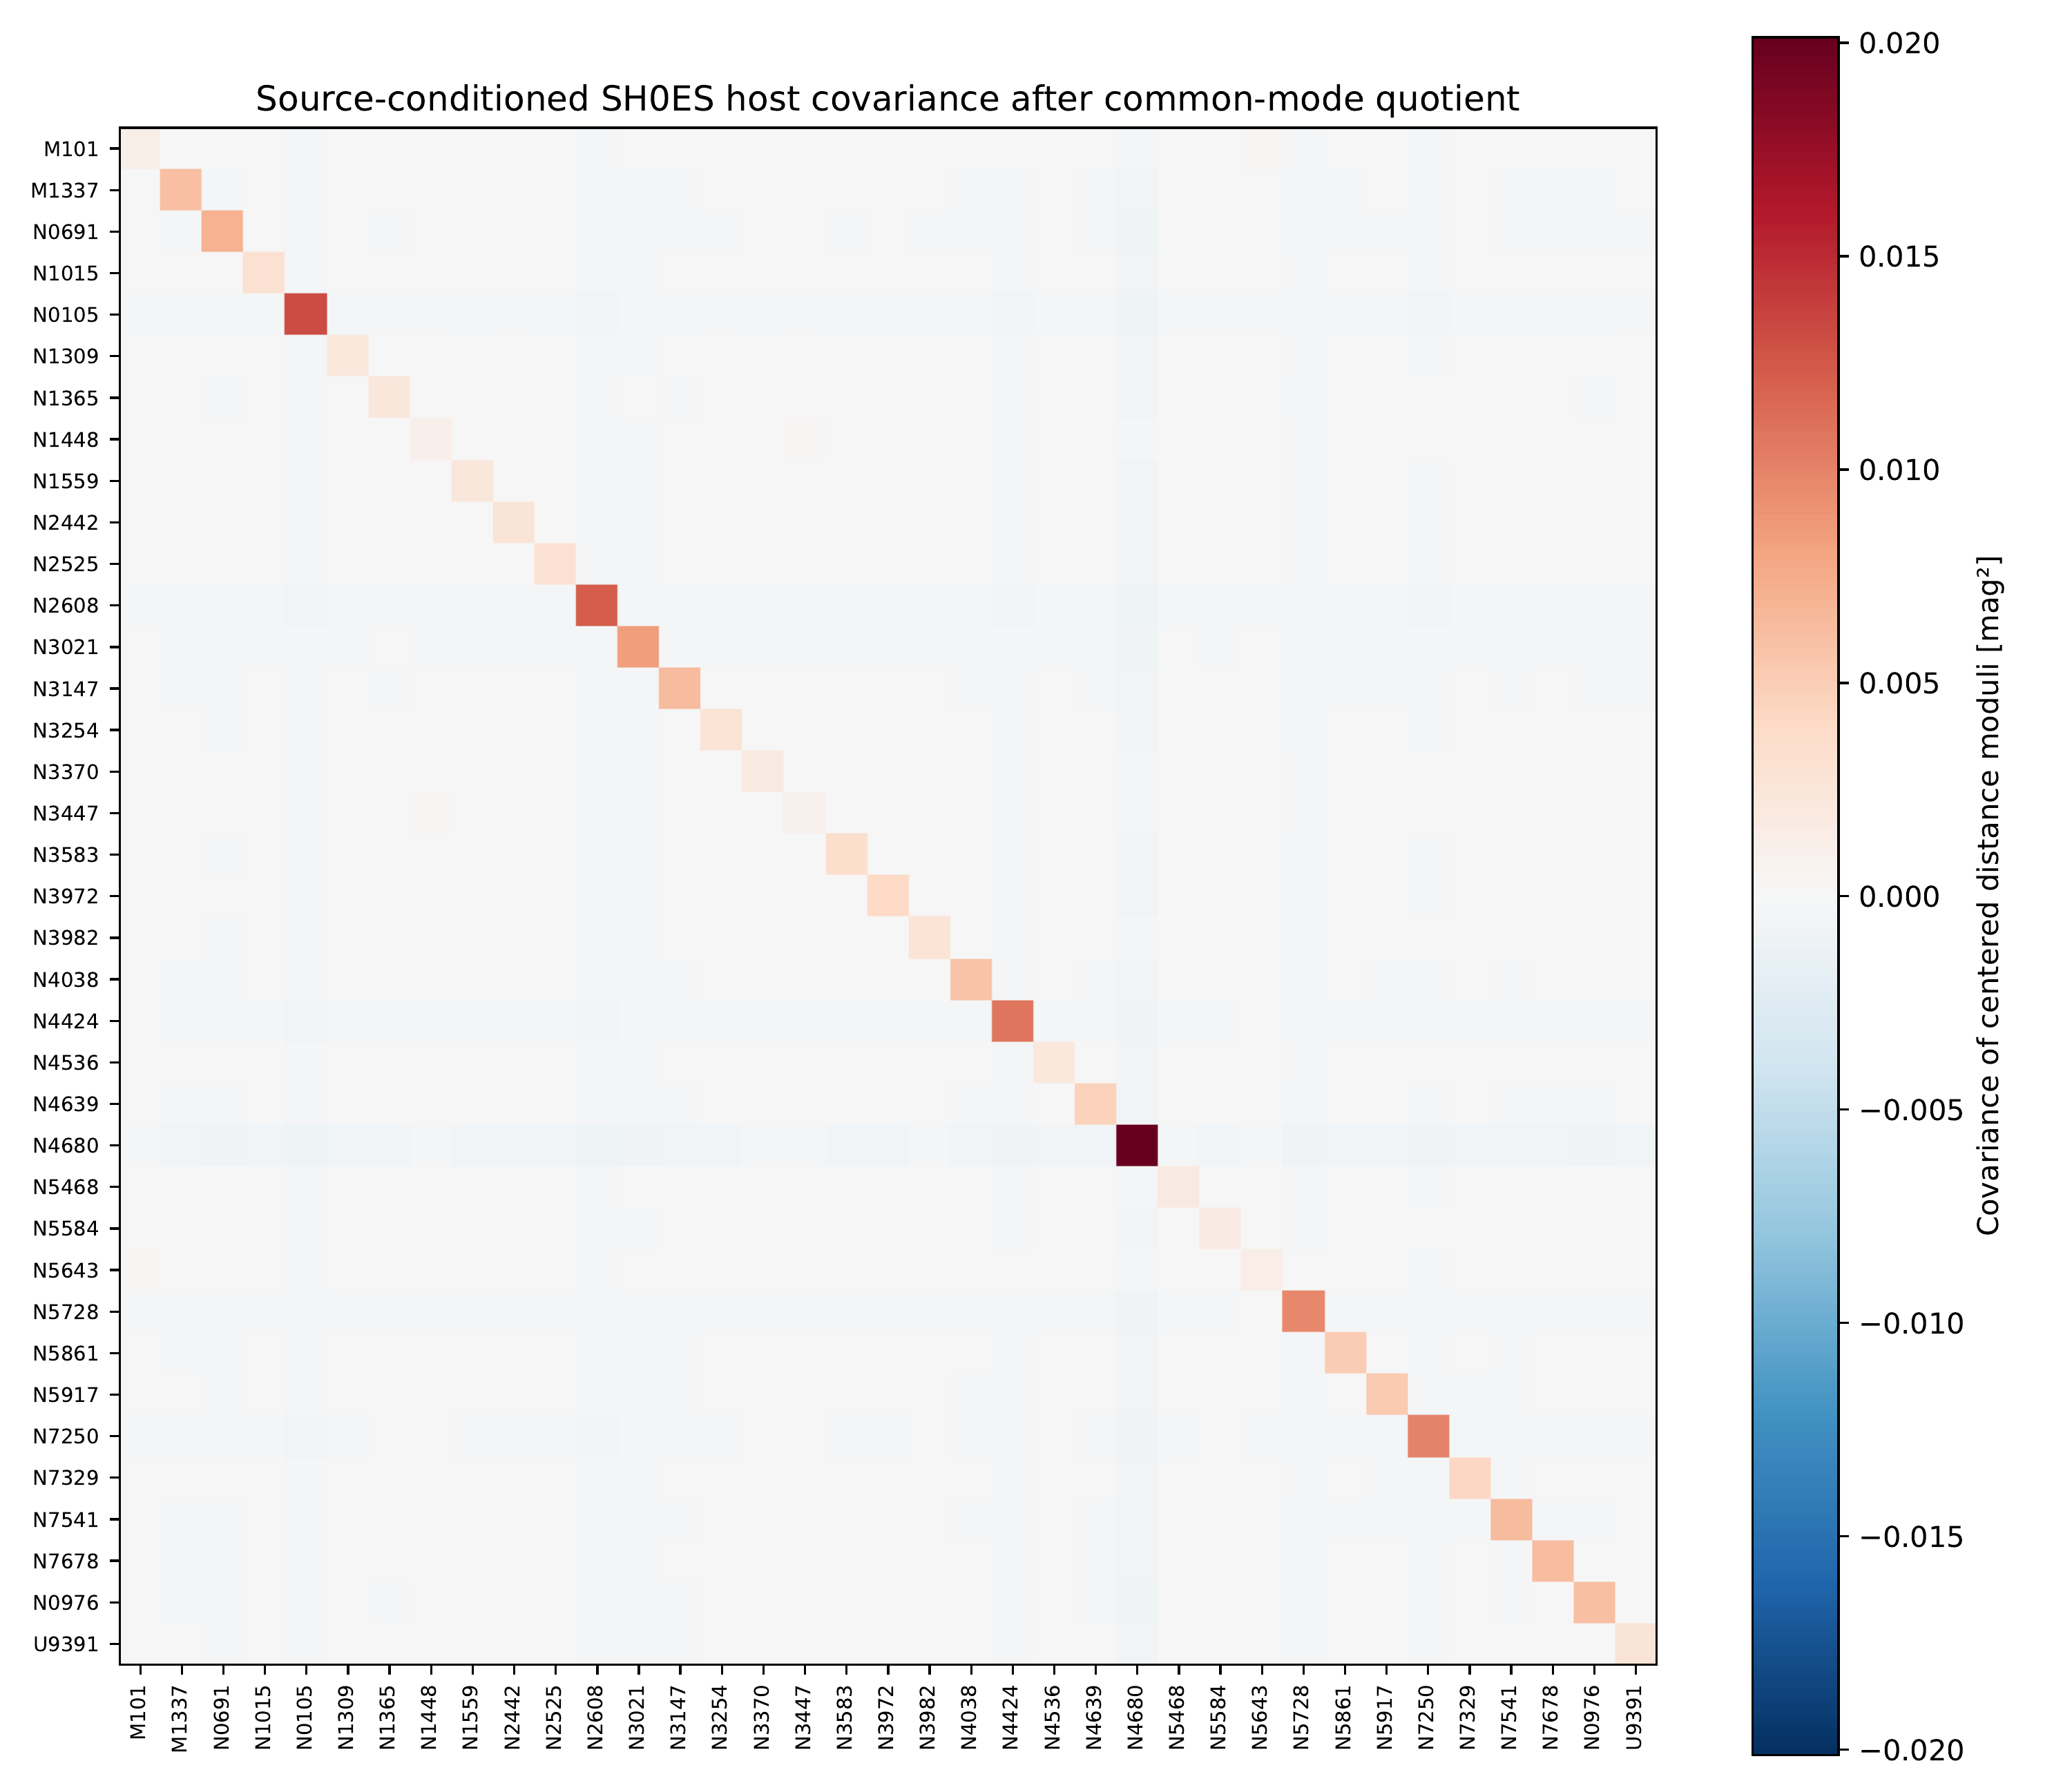
\includegraphics[width=\linewidth,height=.71\textheight,keepaspectratio]{figures/f088_external.png}
\caption{Source-conditioned SH0ES host covariance after the common-mode quotient. The Gaussian ladder reproduction is a source-model check, not a new Hubble-constant measurement. The covariance is not a joint Pantheon+--Cosmicflows source law.}
\label{fig:f088}
\end{figure}
\clearpage
\begin{figure}[p]
\centering
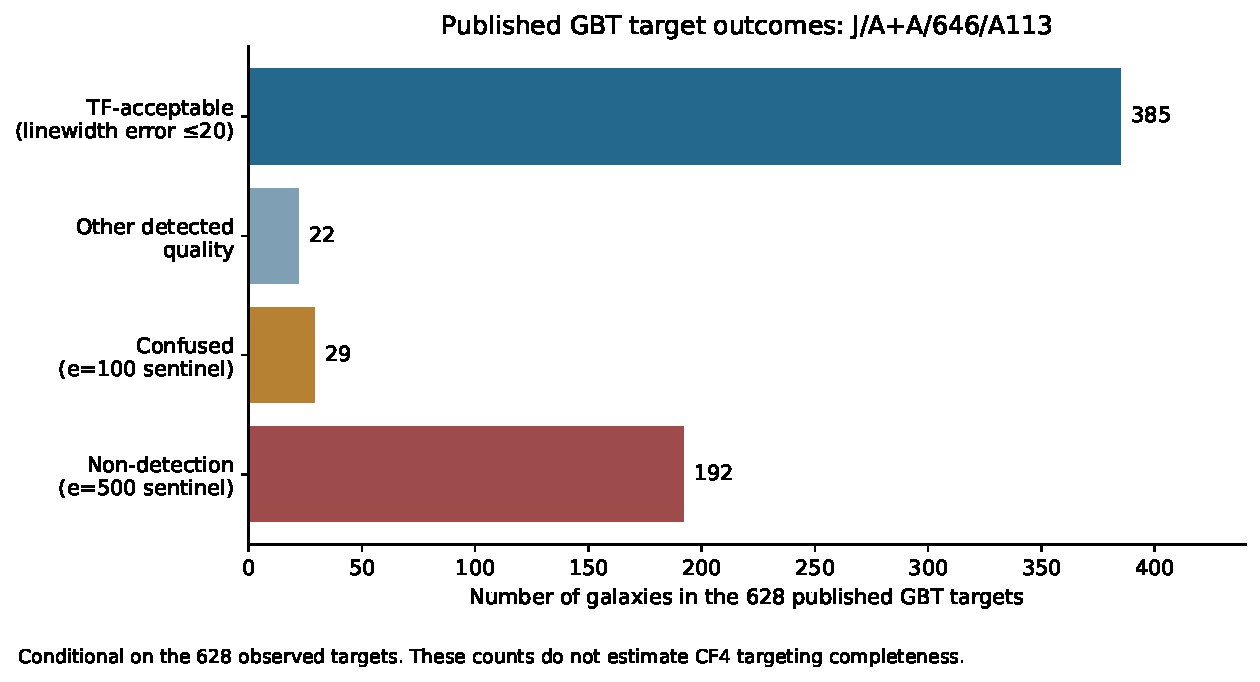
\includegraphics[width=\linewidth,height=.71\textheight,keepaspectratio]{figures/f089.pdf}
\caption{Published hydrogen-line target outcomes. Accepted, other detected, confused, and nondetected objects are distinct observational states. The counts describe the released target sample and are not interchangeable with a later crossmatched distance-bearing cohort.}
\label{fig:f089}
\end{figure}
\clearpage
\begin{figure}[p]
\centering
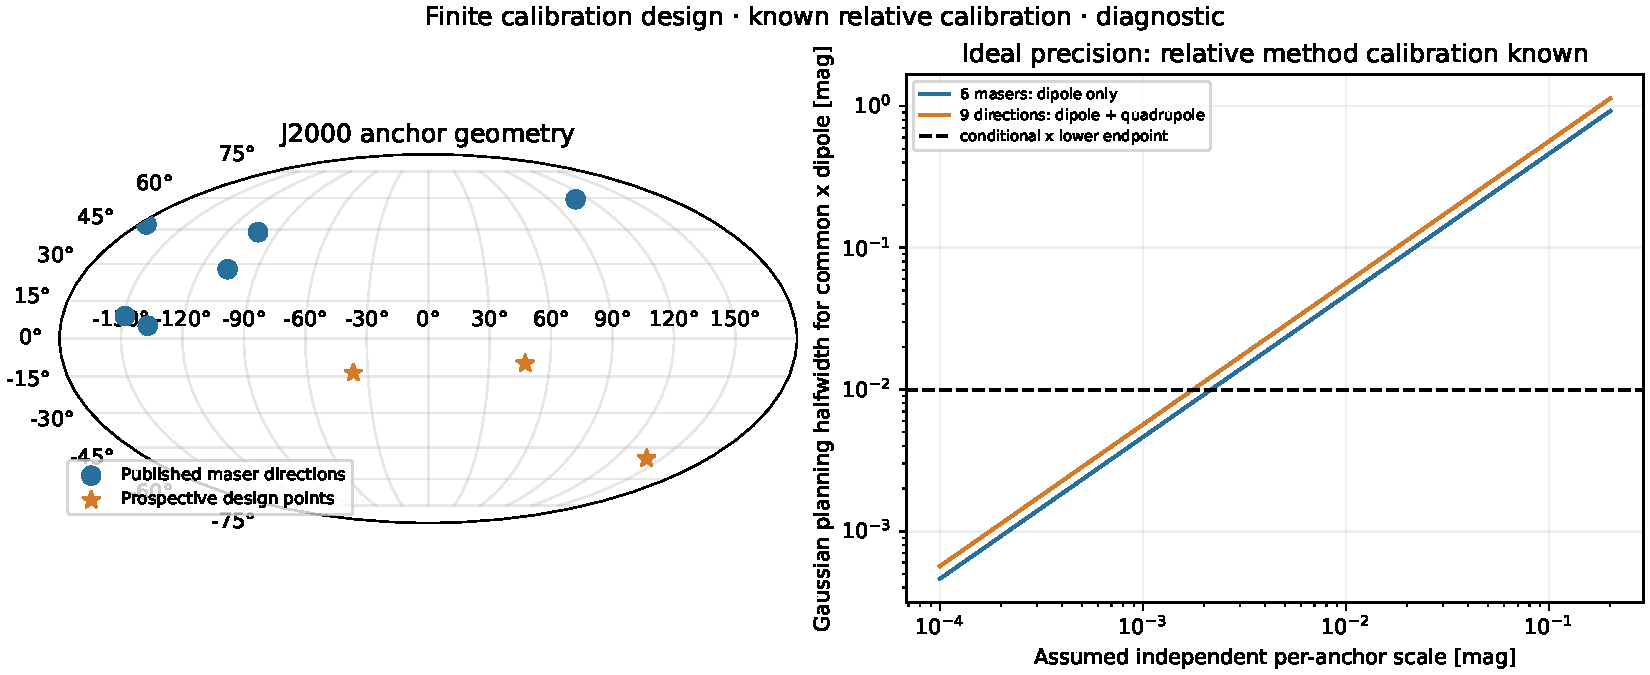
\includegraphics[width=\linewidth,height=.71\textheight,keepaspectratio]{figures/f090_external.pdf}
\caption{Maser-anchor sky geometry and hypothetical precision in six dipole-calibration directions versus nine dipole-plus-quadrupole directions. The source positions determine the geometric design. The precision curves require the stated assumed anchor uncertainties and response model; they are not measured calibration precision or an absolute shear constraint.}
\label{fig:f090}
\end{figure}
\clearpage
\begin{figure}[p]
\centering
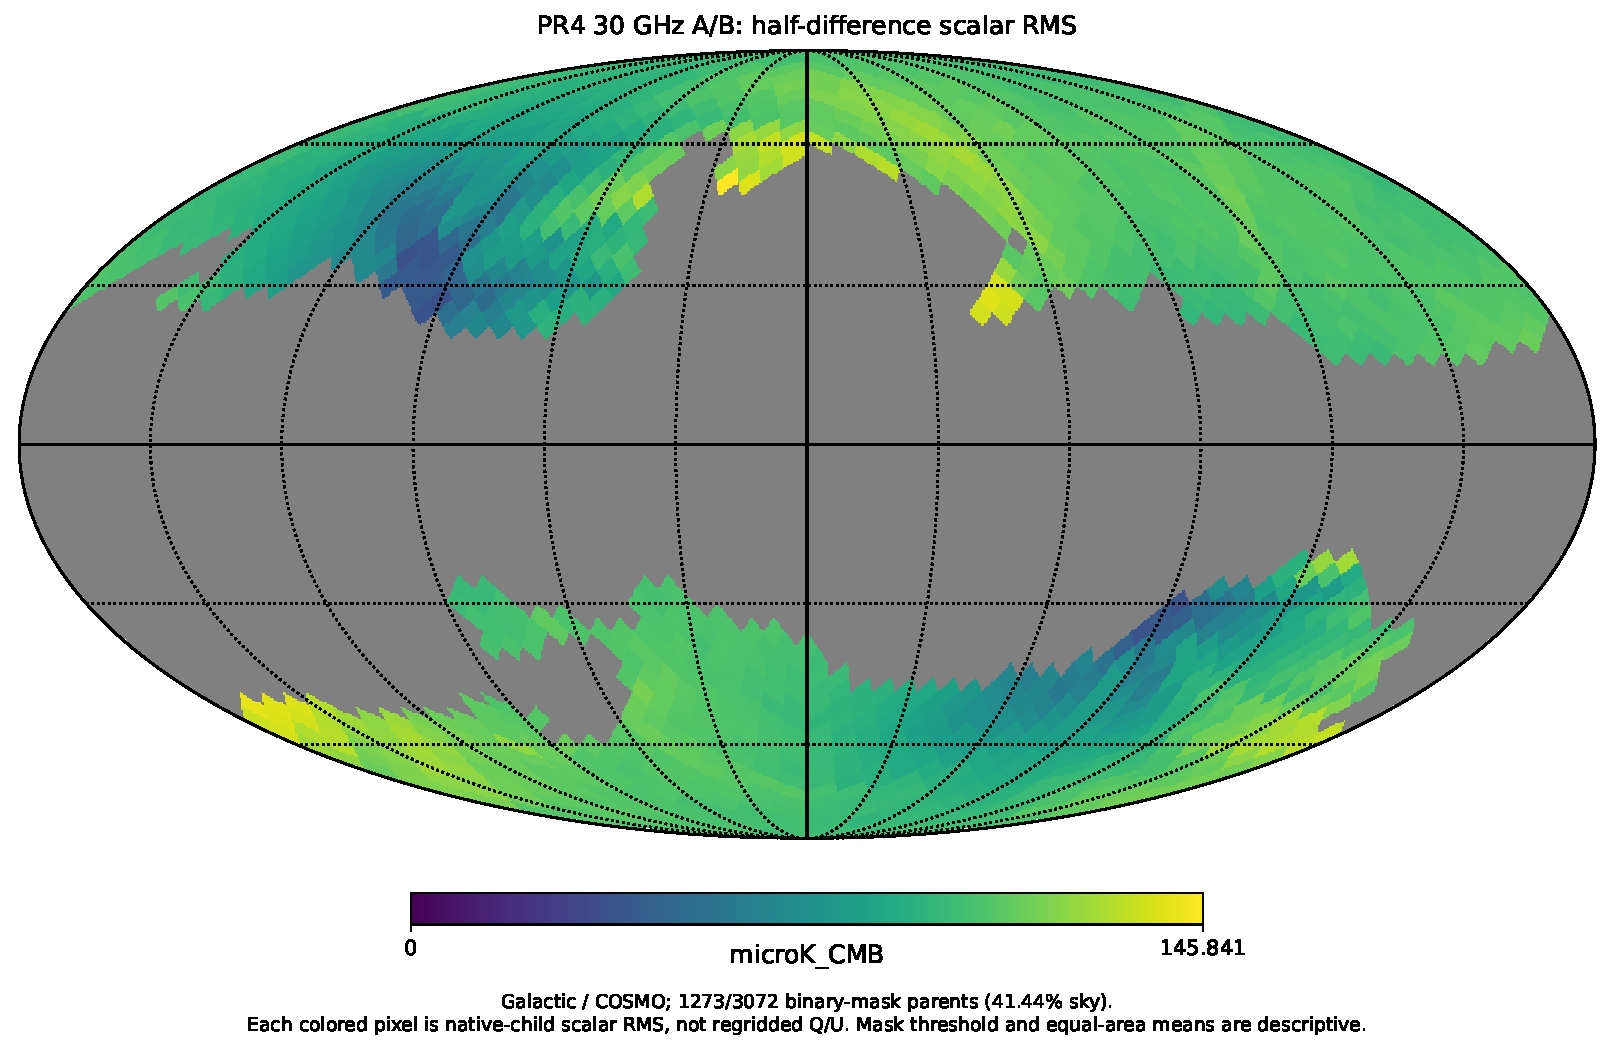
\includegraphics[width=\linewidth,height=.71\textheight,keepaspectratio]{figures/f091.pdf}
\caption{Scalar half-difference RMS for the retained Planck PR4 30-GHz pair. Each displayed cell summarizes original child pixels rather than a downgraded polarization field. Masking and component correlations remain; this is not a noise-fraction map or a calibrated anisotropy test.}
\label{fig:f091}
\end{figure}
\clearpage
\begin{figure}[p]
\centering
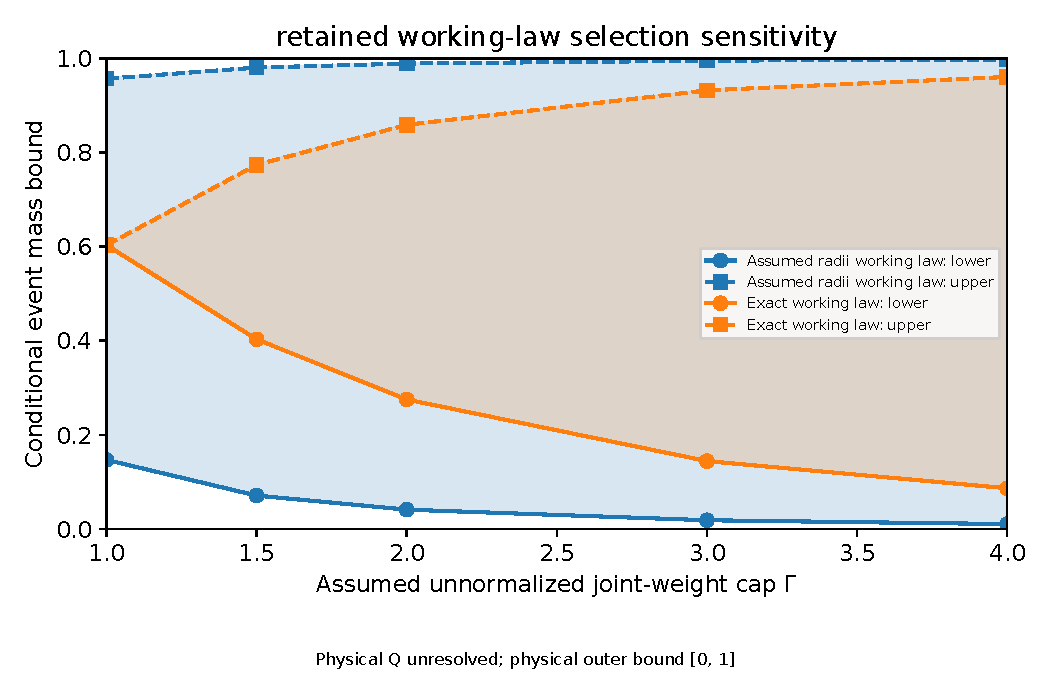
\includegraphics[width=\linewidth,height=.71\textheight,keepaspectratio]{figures/f092_external.pdf}
\caption{Selection sensitivity of the retained coupled finite measure, with exact or assumed-radius event bounds shown separately. The physical selection law is unqualified. Empirical conditional event mass is not a physical posterior or a null probability.}
\label{fig:f092}
\end{figure}
\clearpage
\begin{figure}[p]
\centering
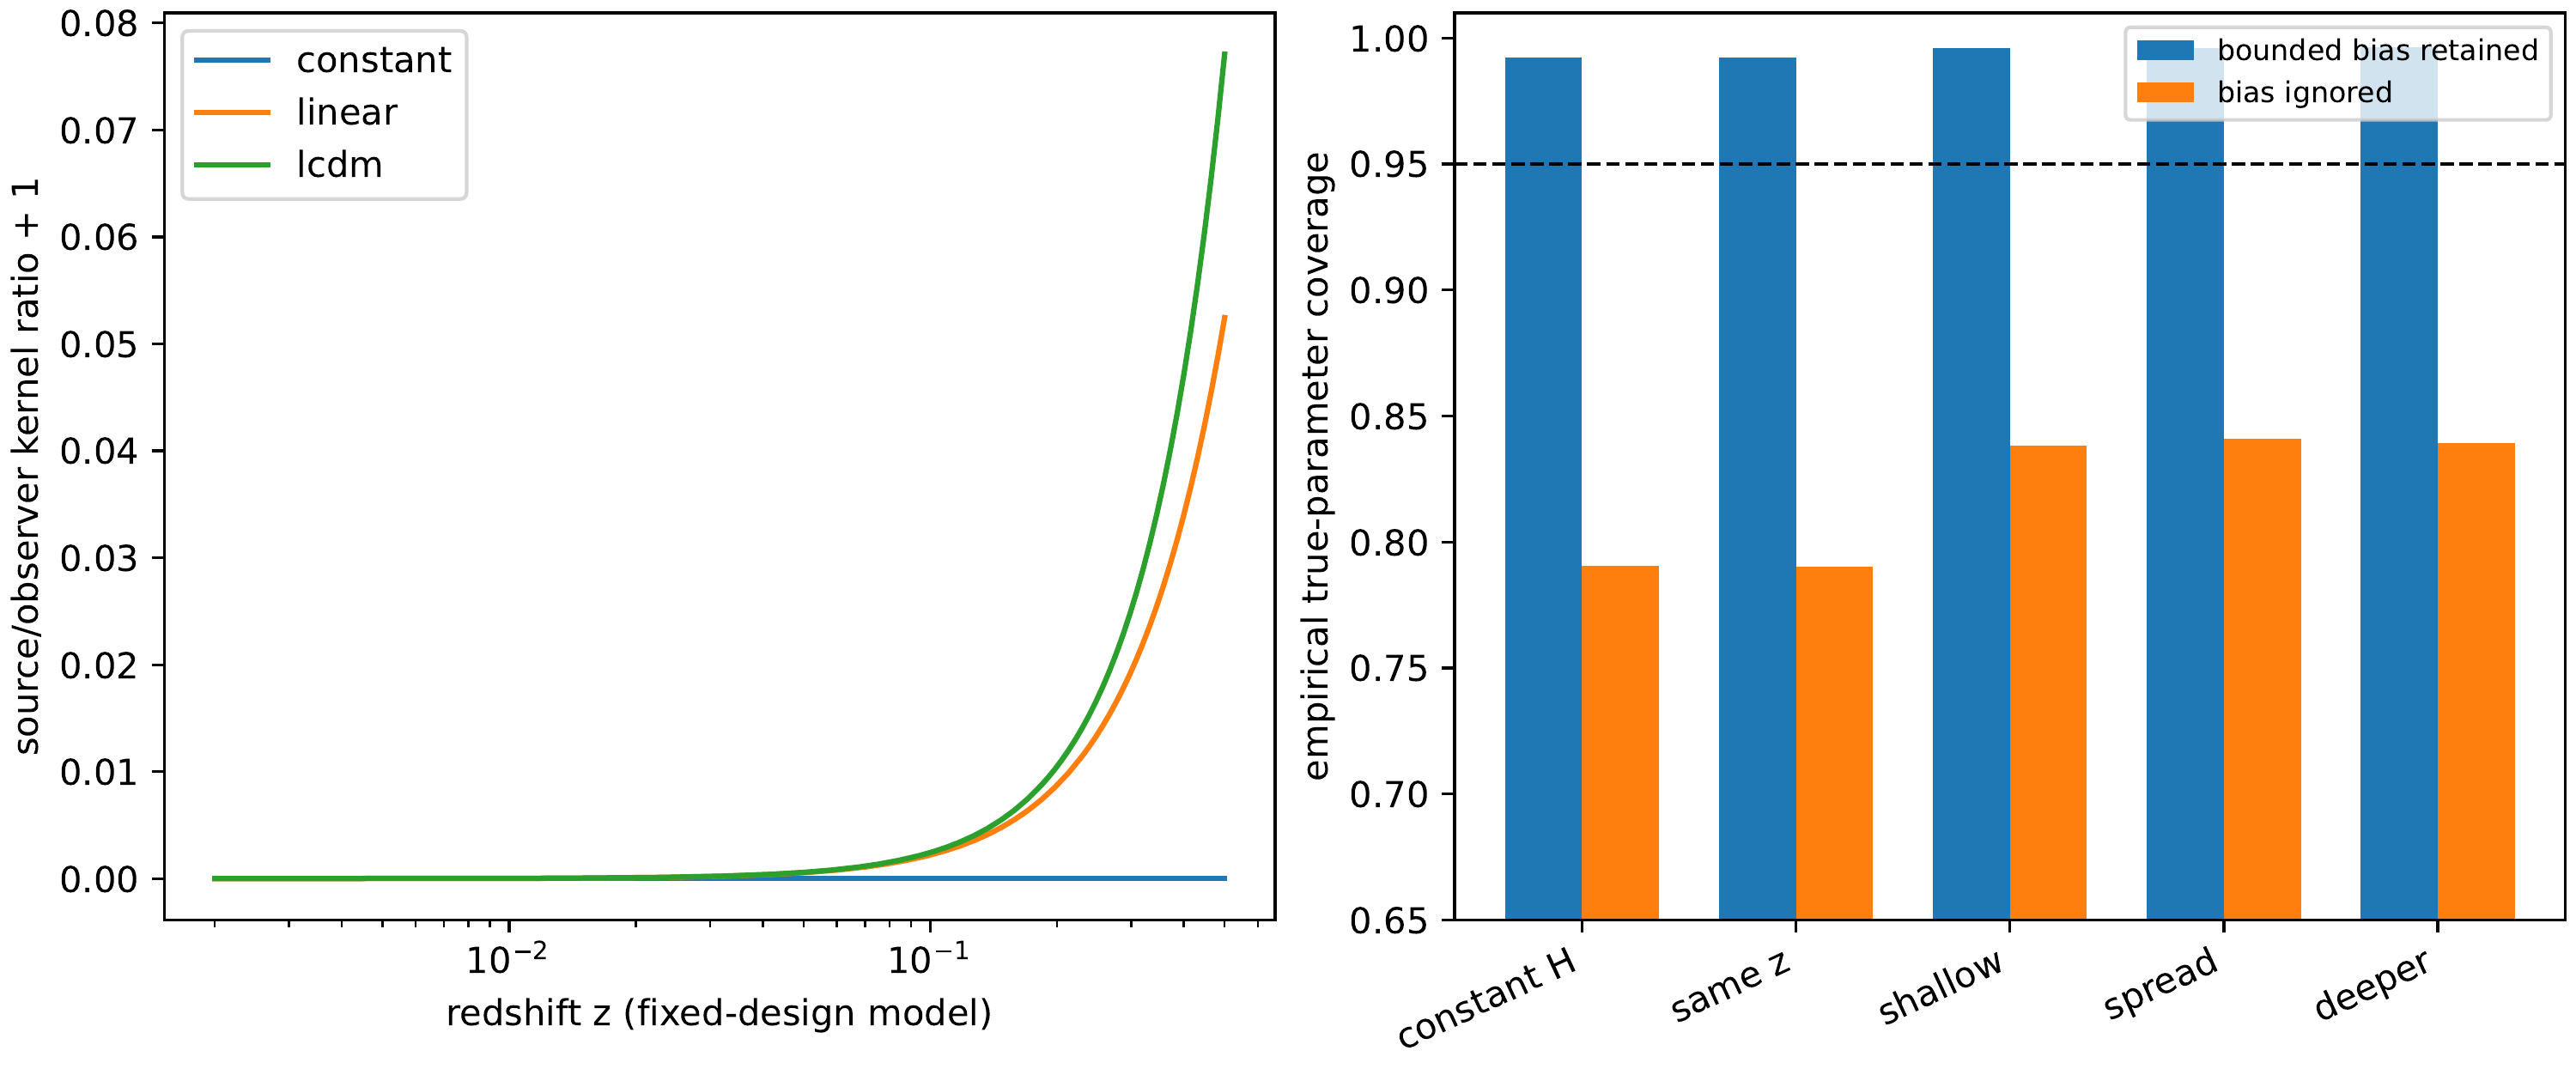
\includegraphics[width=\linewidth,height=.71\textheight,keepaspectratio]{figures/f093_external.png}
\caption{Synthetic fixed-design response and coverage controls for tensor inference. The response ratios and coverage frequencies concern the explicitly generated model. They are not observational constraints or evidence of physical source-law validity.}
\label{fig:f093}
\end{figure}
\clearpage
\begin{figure}[p]
\centering
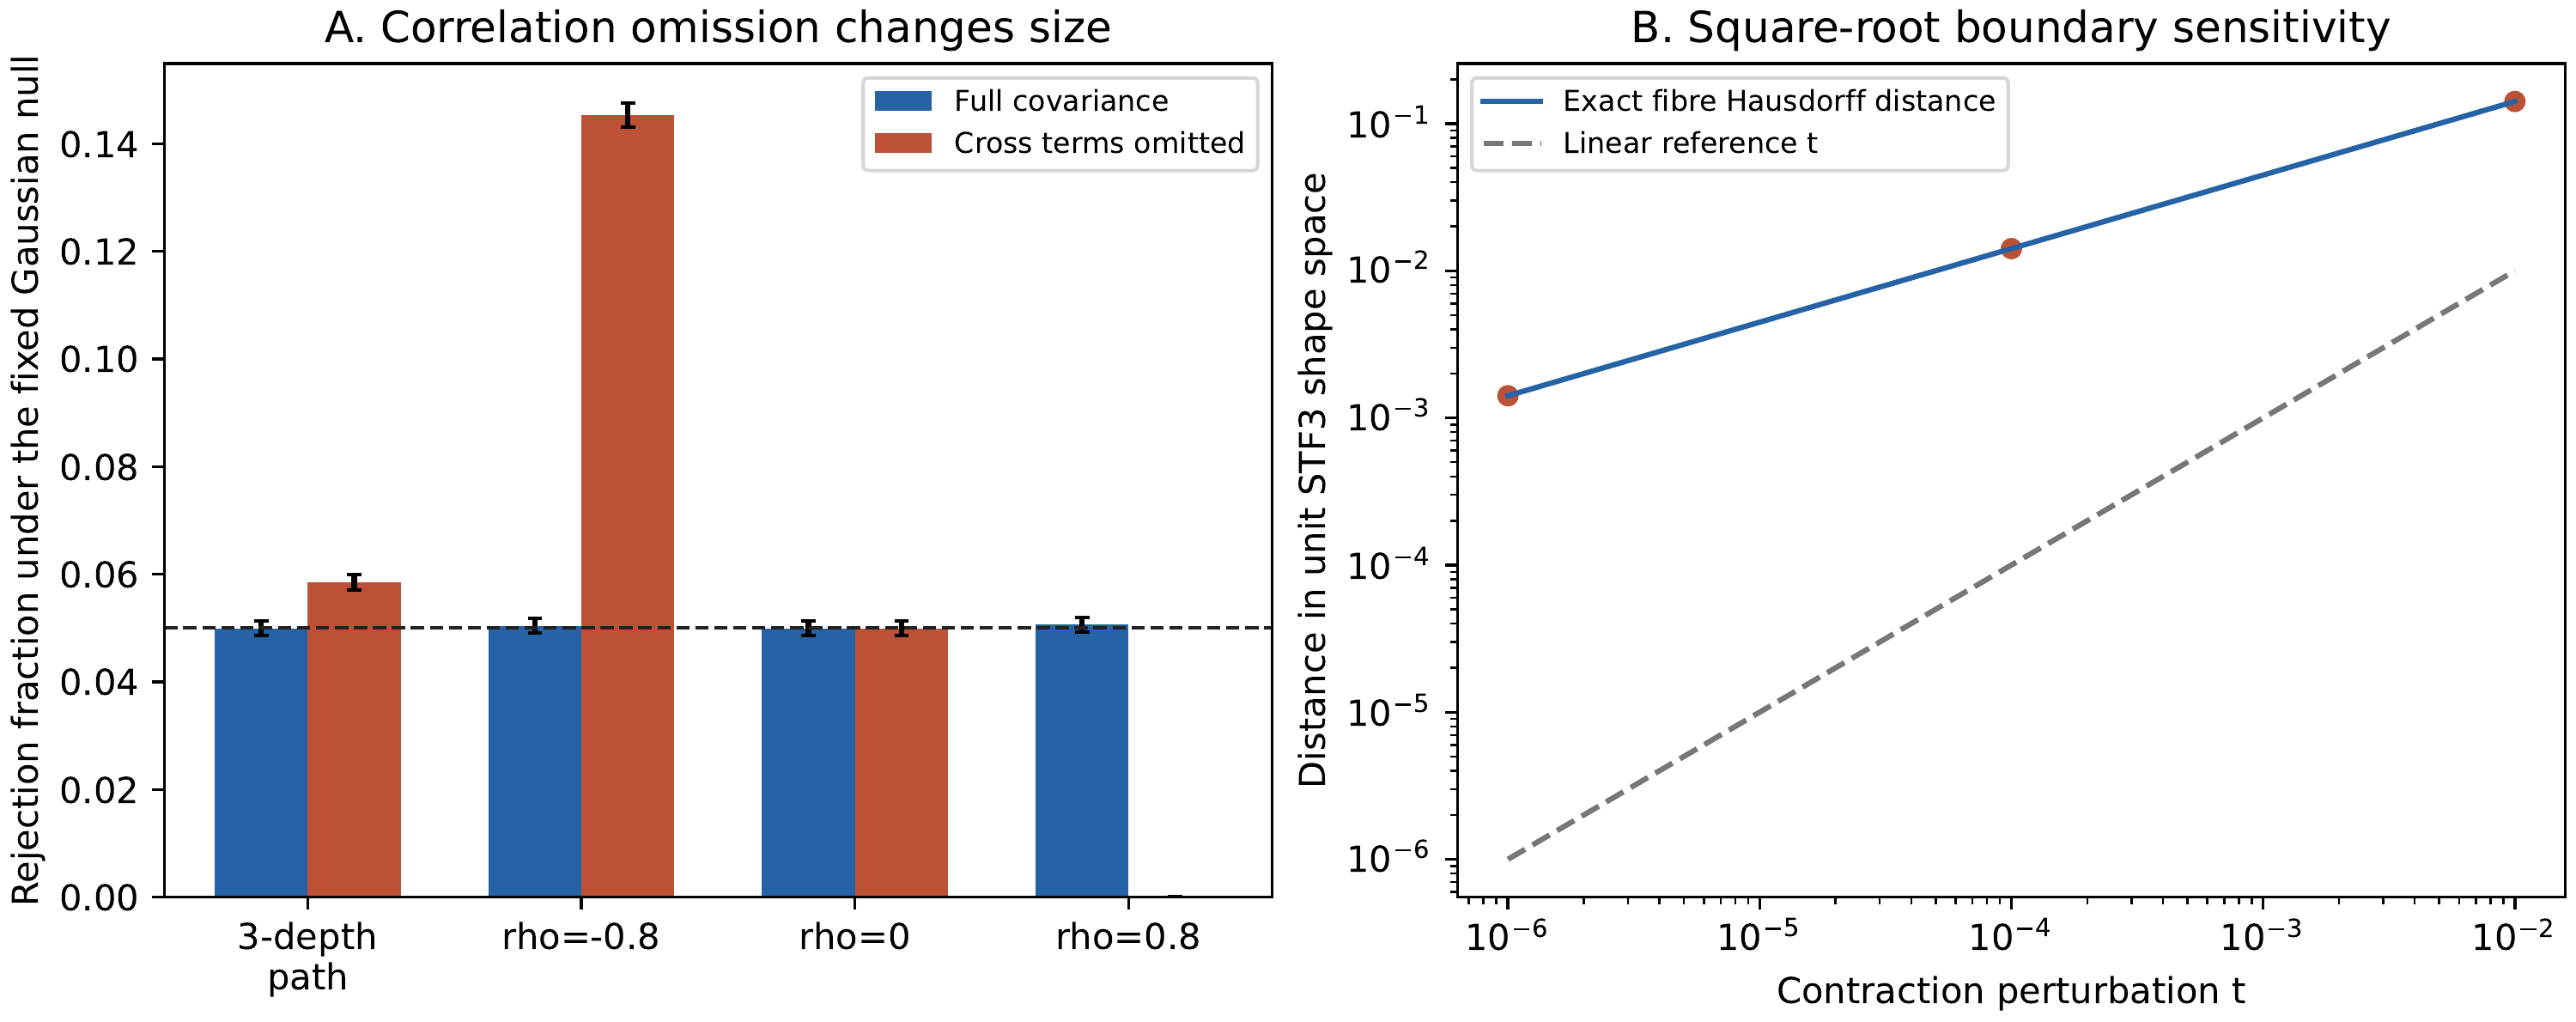
\includegraphics[width=\linewidth,height=.71\textheight,keepaspectratio]{figures/f094_external.png}
\caption{Synthetic controls for omitted covariance, nonlinear boundaries, and joint tensor images. Dropping cross terms changes error rates, and square-root boundaries invalidate an unqualified linear approximation. These controls motivate retention of the full state and support; they are not additional observations.}
\label{fig:f094}
\end{figure}
\clearpage
\begin{figure}[p]
\centering
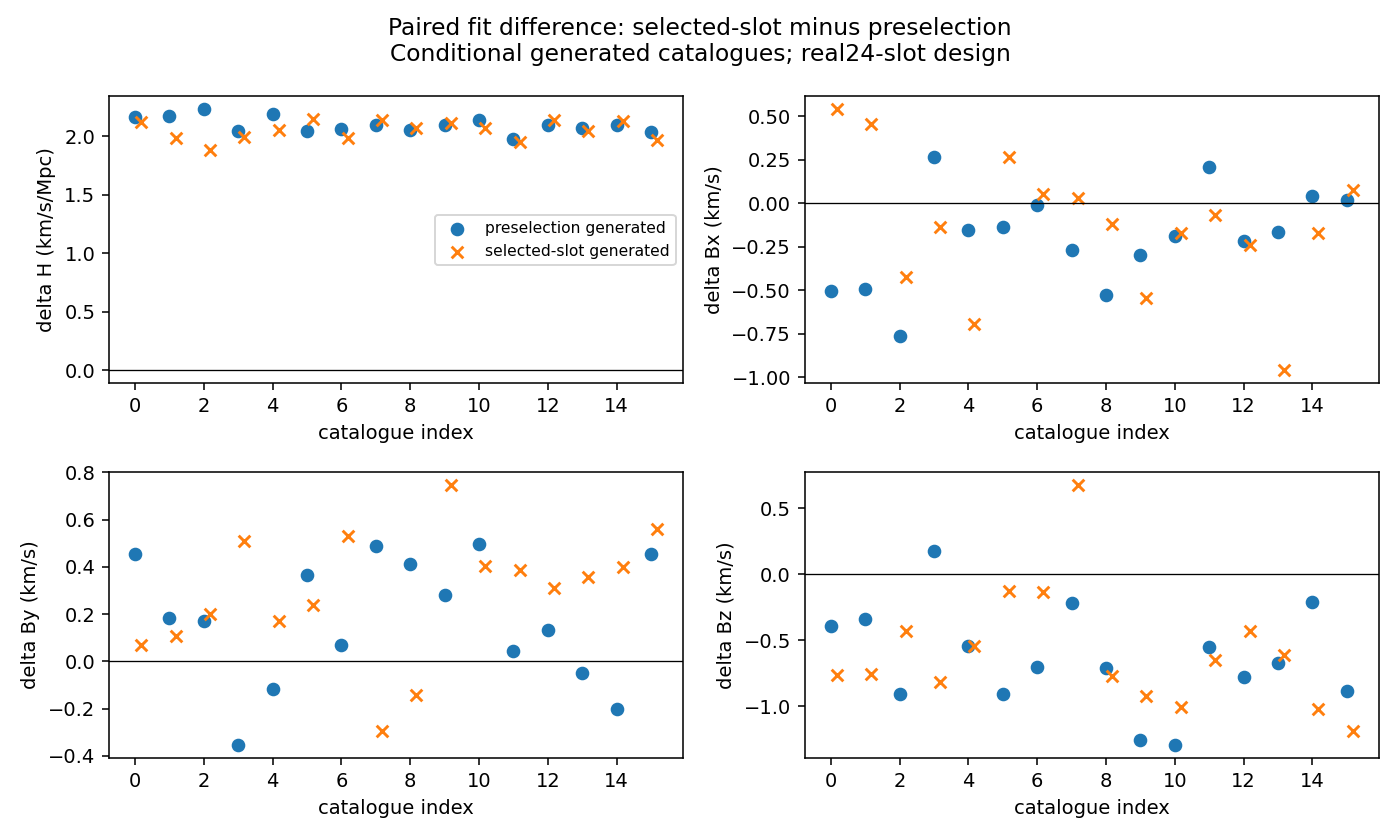
\includegraphics[width=\linewidth,height=.71\textheight,keepaspectratio]{figures/f096.png}
\caption{Paired generated Cosmicflows catalogues under distinct declared source laws. Differences between laws are kept separate from within-law sampling variation. This preview does not identify the actual catalogue selection or physical uncertainty model.}
\label{fig:f096}
\end{figure}
\clearpage
\begin{figure}[p]
\centering
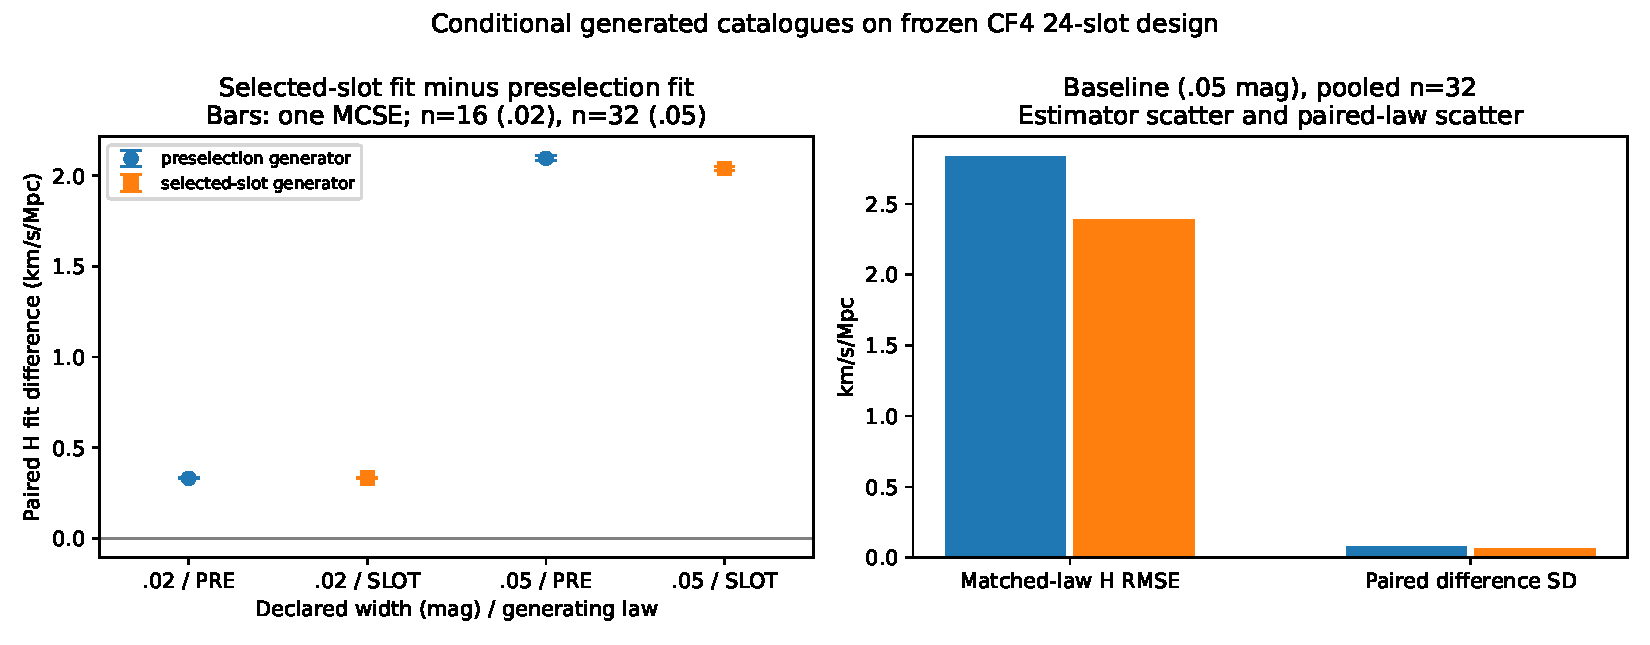
\includegraphics[width=\linewidth,height=.71\textheight,keepaspectratio]{figures/f097.pdf}
\caption{Conditional generated-catalogue precision on a frozen Cosmicflows design. Preselection and selected-slot generators are different experiments. Increasing replication narrows simulation scatter without validating either generator as the observed source law.}
\label{fig:f097}
\end{figure}
\clearpage
\begin{figure}[p]
\centering
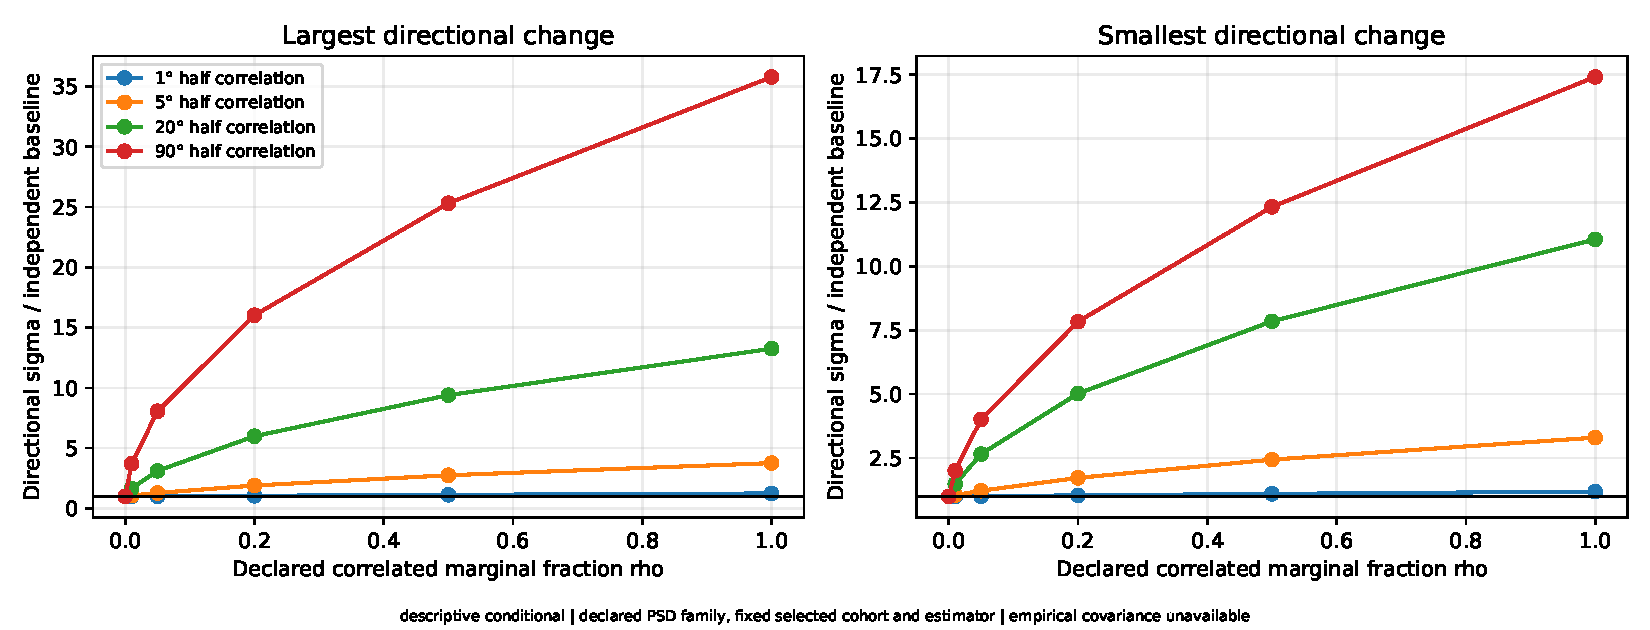
\includegraphics[width=\linewidth,height=.71\textheight,keepaspectratio]{figures/f098_external.pdf}
\caption{Angular-correlation sensitivity in a fixed Gaia source design. The specified correlation families are scenarios. They show dependence of inference on covariance assumptions rather than measuring the actual sky correlation law.}
\label{fig:f098}
\end{figure}
\clearpage
\begin{figure}[p]
\centering
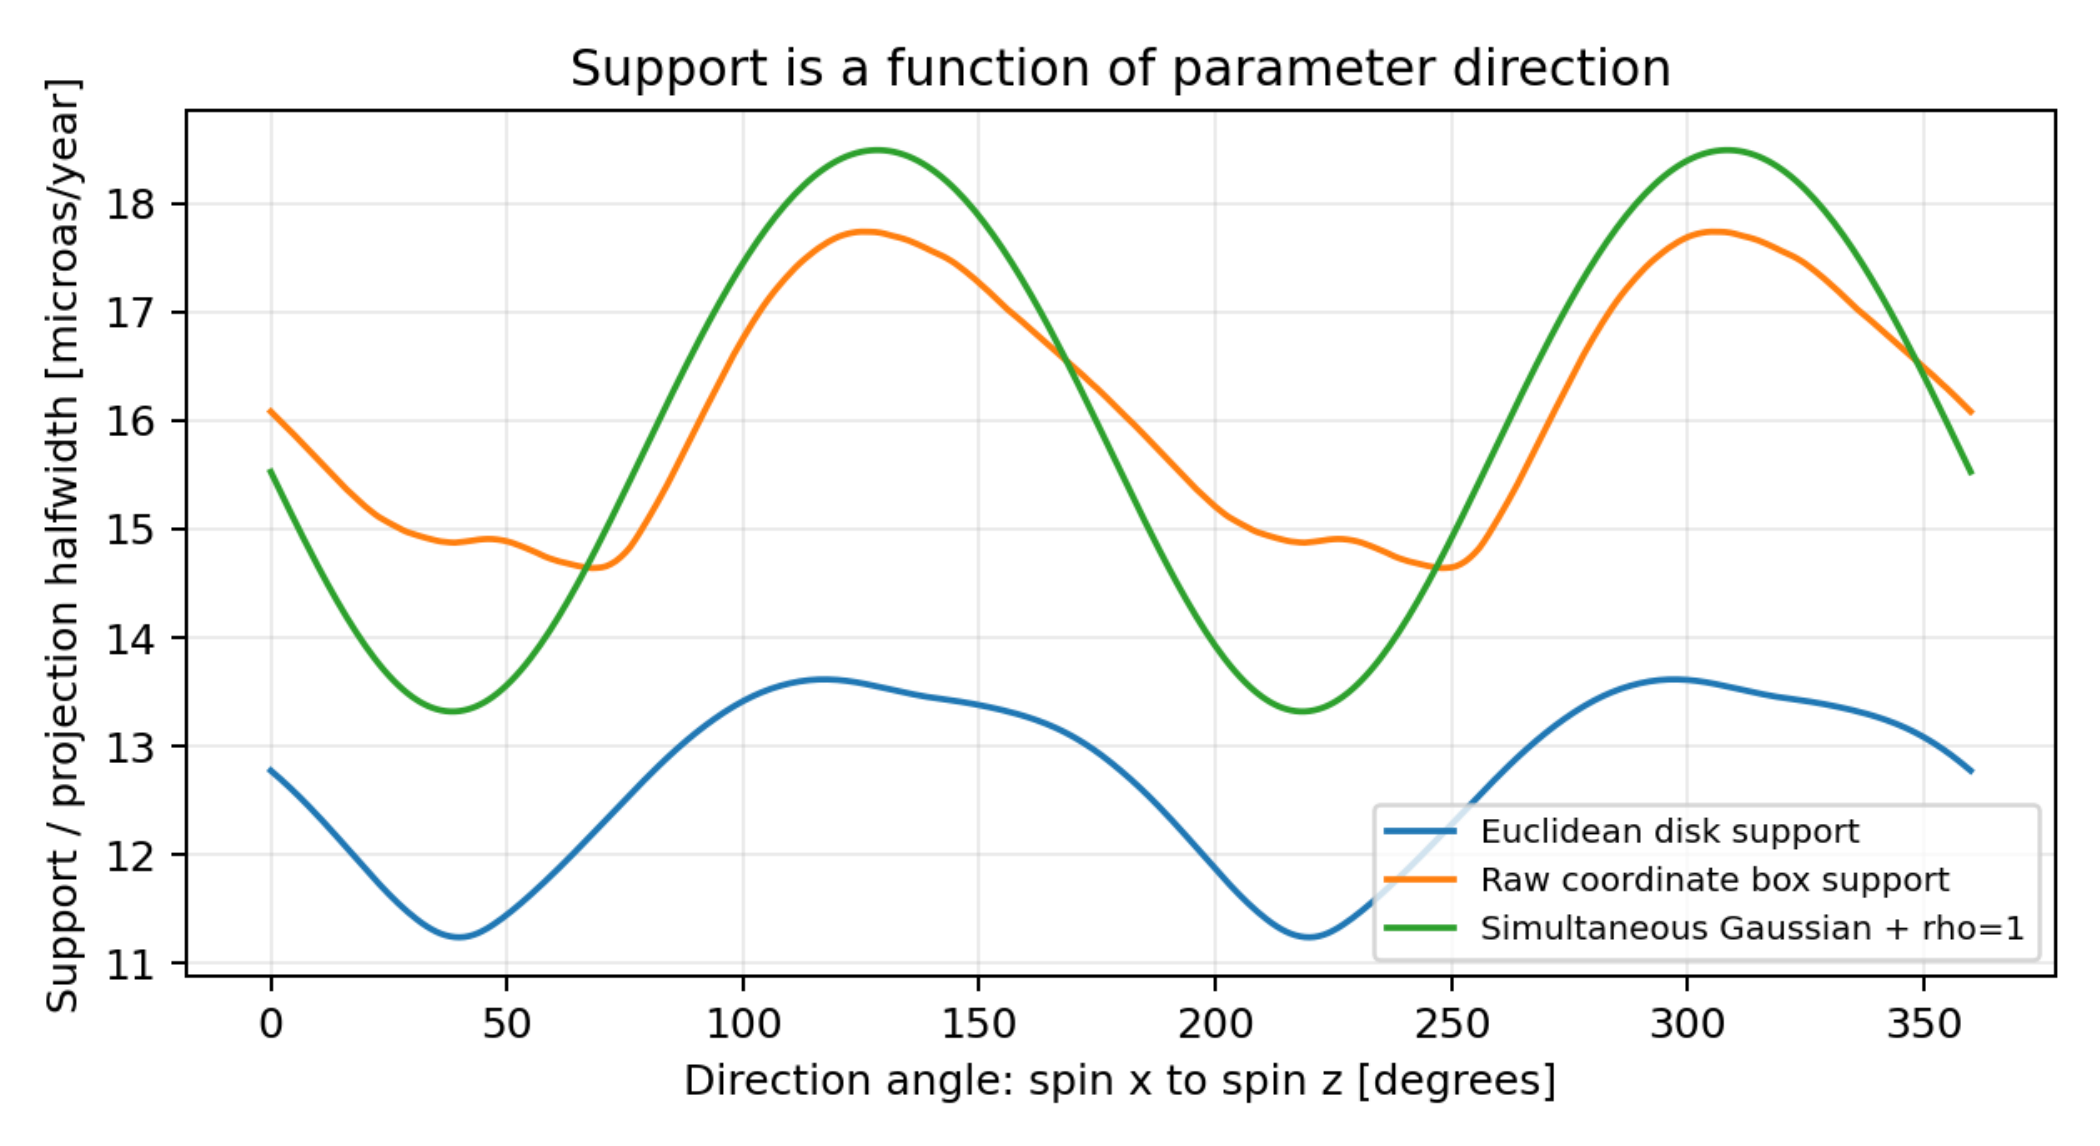
\includegraphics[width=\linewidth,height=.71\textheight,keepaspectratio]{figures/f099_external.png}
\caption{Directional support of a fixed astrometric proxy experiment. The complete operator and state define the plotted support. This geometry does not establish physical Gaia coverage, a matter-following source response, or a probability within the support.}
\label{fig:f099}
\end{figure}
\clearpage
\begin{figure}[p]
\centering
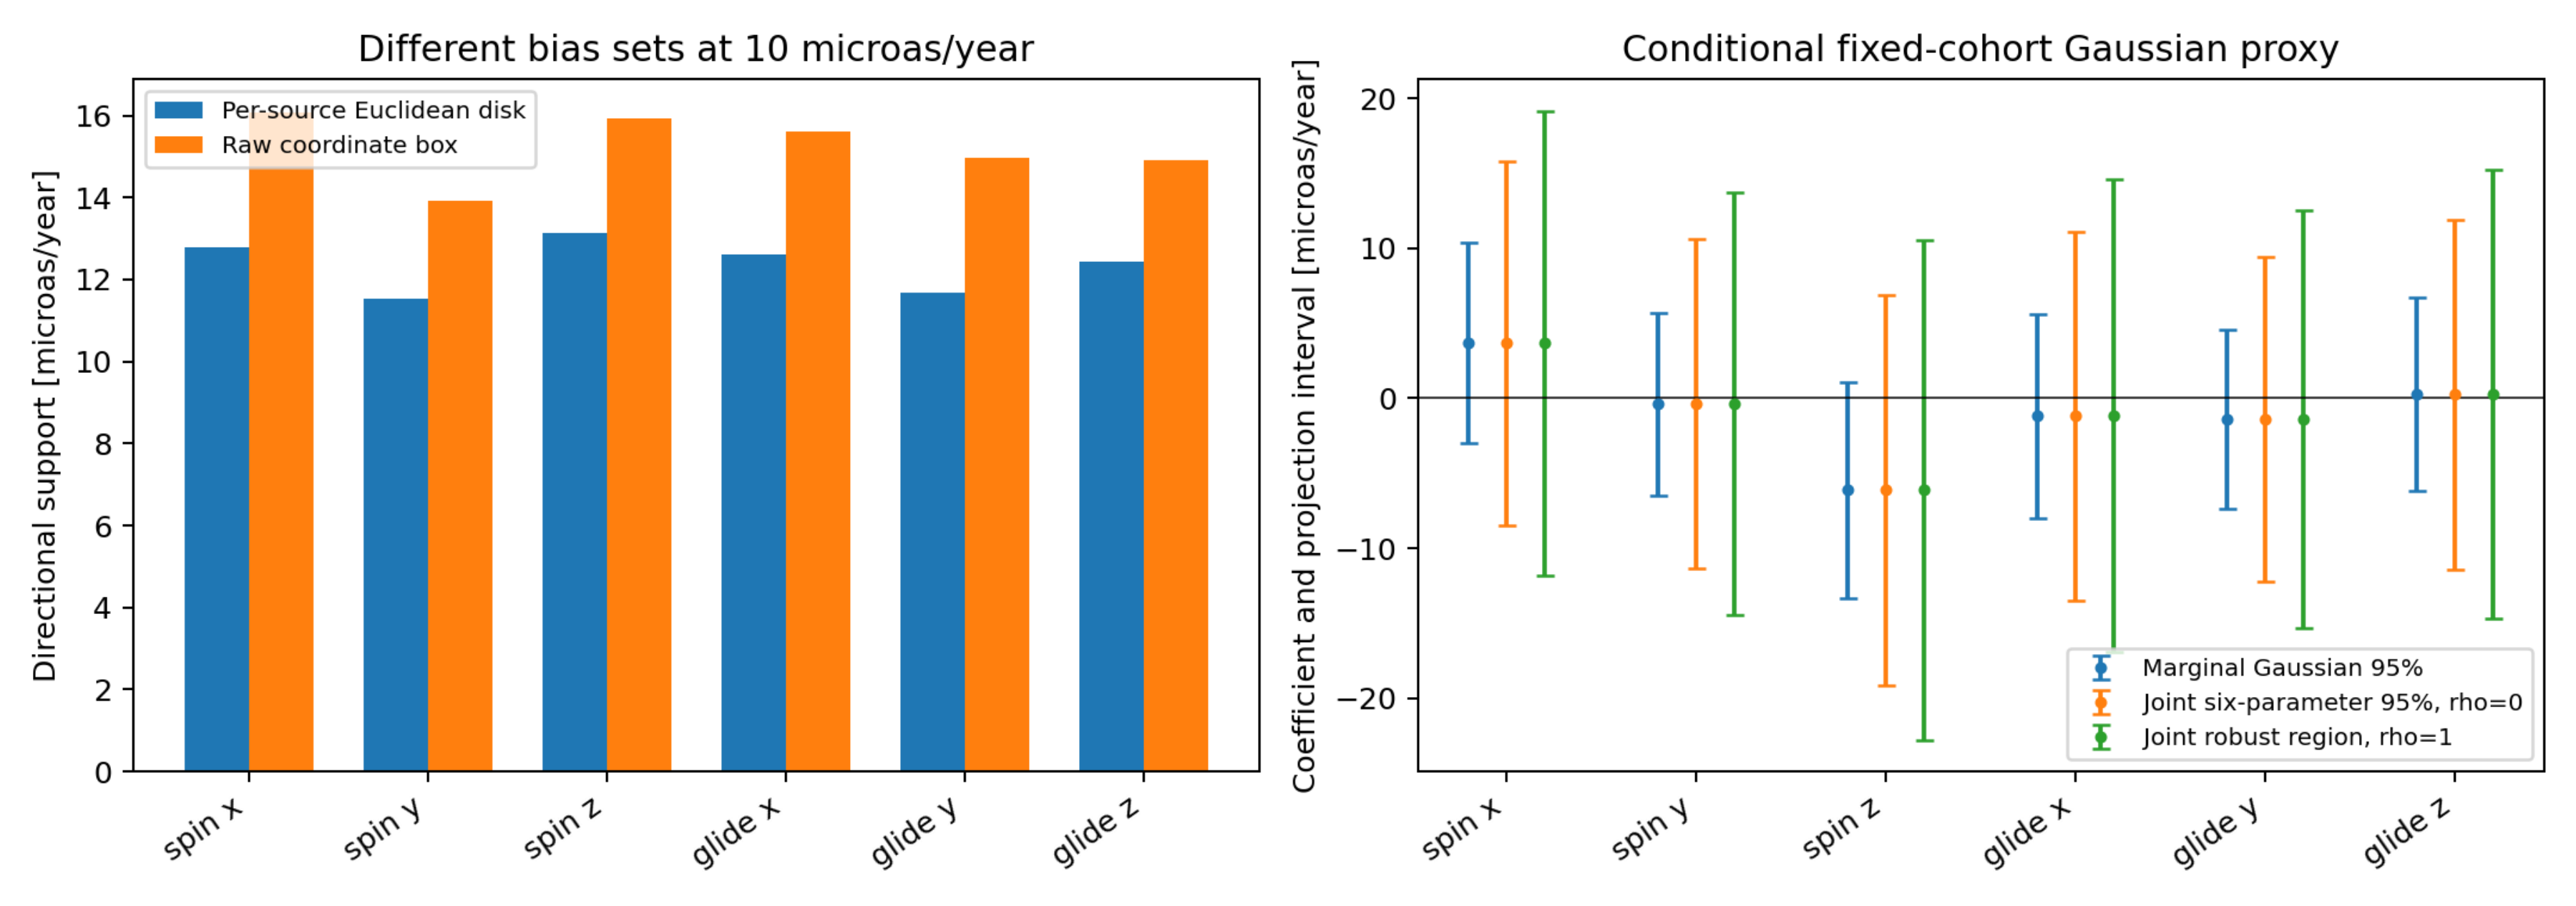
\includegraphics[width=\linewidth,height=.71\textheight,keepaspectratio]{figures/f100_external.png}
\caption{Euclidean-disk and coordinate-box bias supports for the fixed astrometric proxy design, together with marginal and joint Gaussian proxy intervals. The support geometry changes the allowed image even at the same coordinate scale. The assumed bias sets and Gaussian law do not establish physical Gaia uncertainty or population coverage.}
\label{fig:f100}
\end{figure}
\clearpage
\begin{figure}[p]
\centering
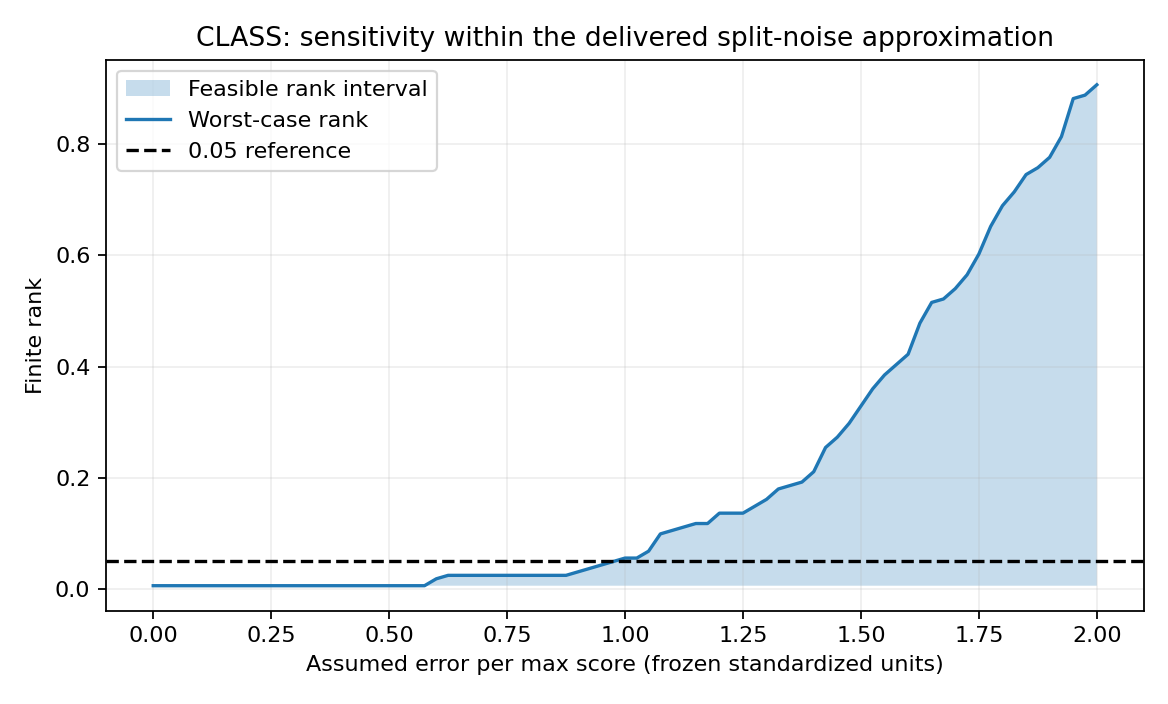
\includegraphics[width=\linewidth,height=.71\textheight,keepaspectratio]{figures/f101.png}
\caption{Finite tail-rank sensitivity for the CLASS split-noise comparison with 160 reference scores. The interval widens as an assumed error allowance is applied to the observed and reference scores. This allowance is not a measured physical systematic bound. Finite rank arithmetic does not establish exchangeability or turn the split-noise approximation into a physical null law.}
\label{fig:f101}
\end{figure}
\clearpage
\begin{figure}[p]
\centering
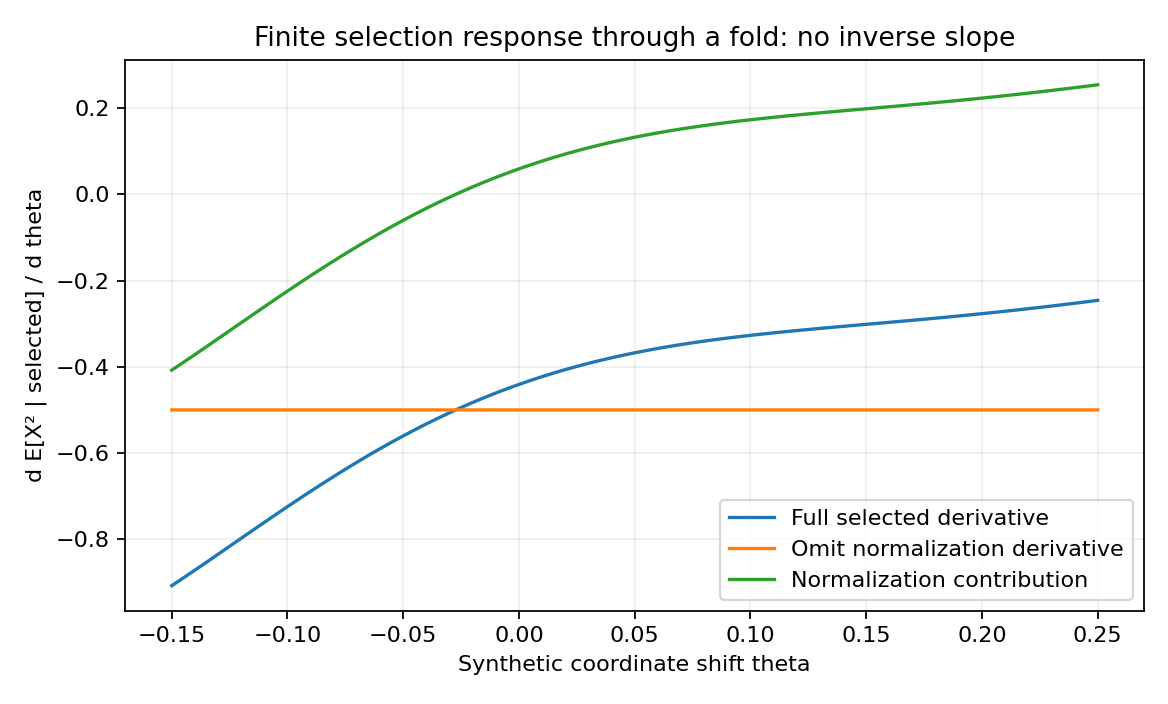
\includegraphics[width=\linewidth,height=.71\textheight,keepaspectratio]{figures/f102.png}
\caption{A synthetic nonlinear selection response: X is uniform on [-1,1], the latent quantity is X squared plus theta, and Gaussian measurement noise has standard deviation 0.1; observations are selected between -0.1 and 0.4. The derivative of the selected mean of X squared includes the derivative of the selection normalization. The curves concern this dimensionless generated model, not cross-validation or an observed catalogue fit.}
\label{fig:f102}
\end{figure}
\clearpage
\begin{figure}[p]
\centering
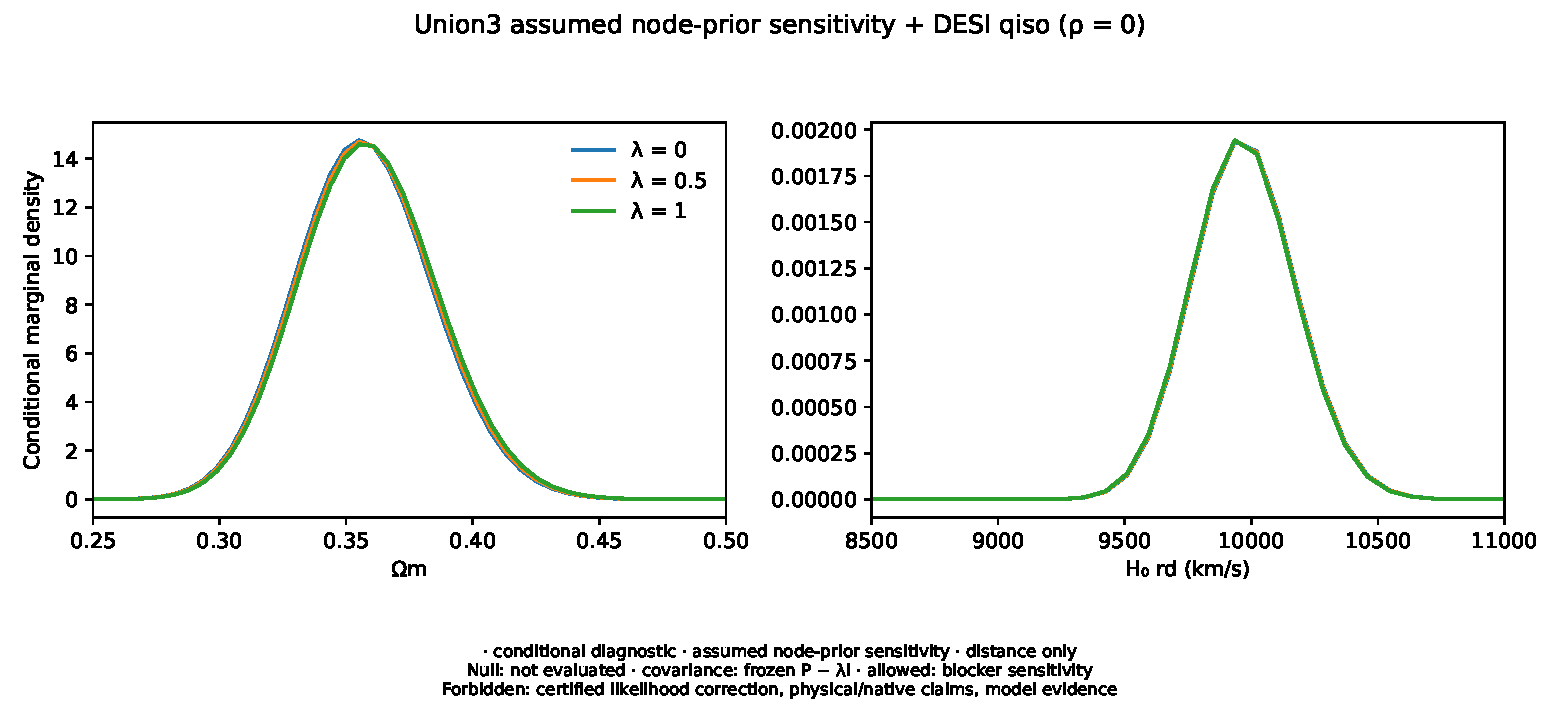
\includegraphics[width=\linewidth,height=.71\textheight,keepaspectratio]{figures/f103_external.pdf}
\caption{Union3 and DESI distance sensitivity to removal of an assumed Gaussian distance-node prior, with removal fractions zero, one-half, and one and cross-source correlation fixed to zero. The scenario marginals depend on that assumed prior and source precision. The exact released-matrix relation to the published prior and public code remains unresolved, so these curves are not a certified correction to the released likelihood or a cross-scenario evidence comparison.}
\label{fig:f103}
\end{figure}
\clearpage
\begin{figure}[p]
\centering
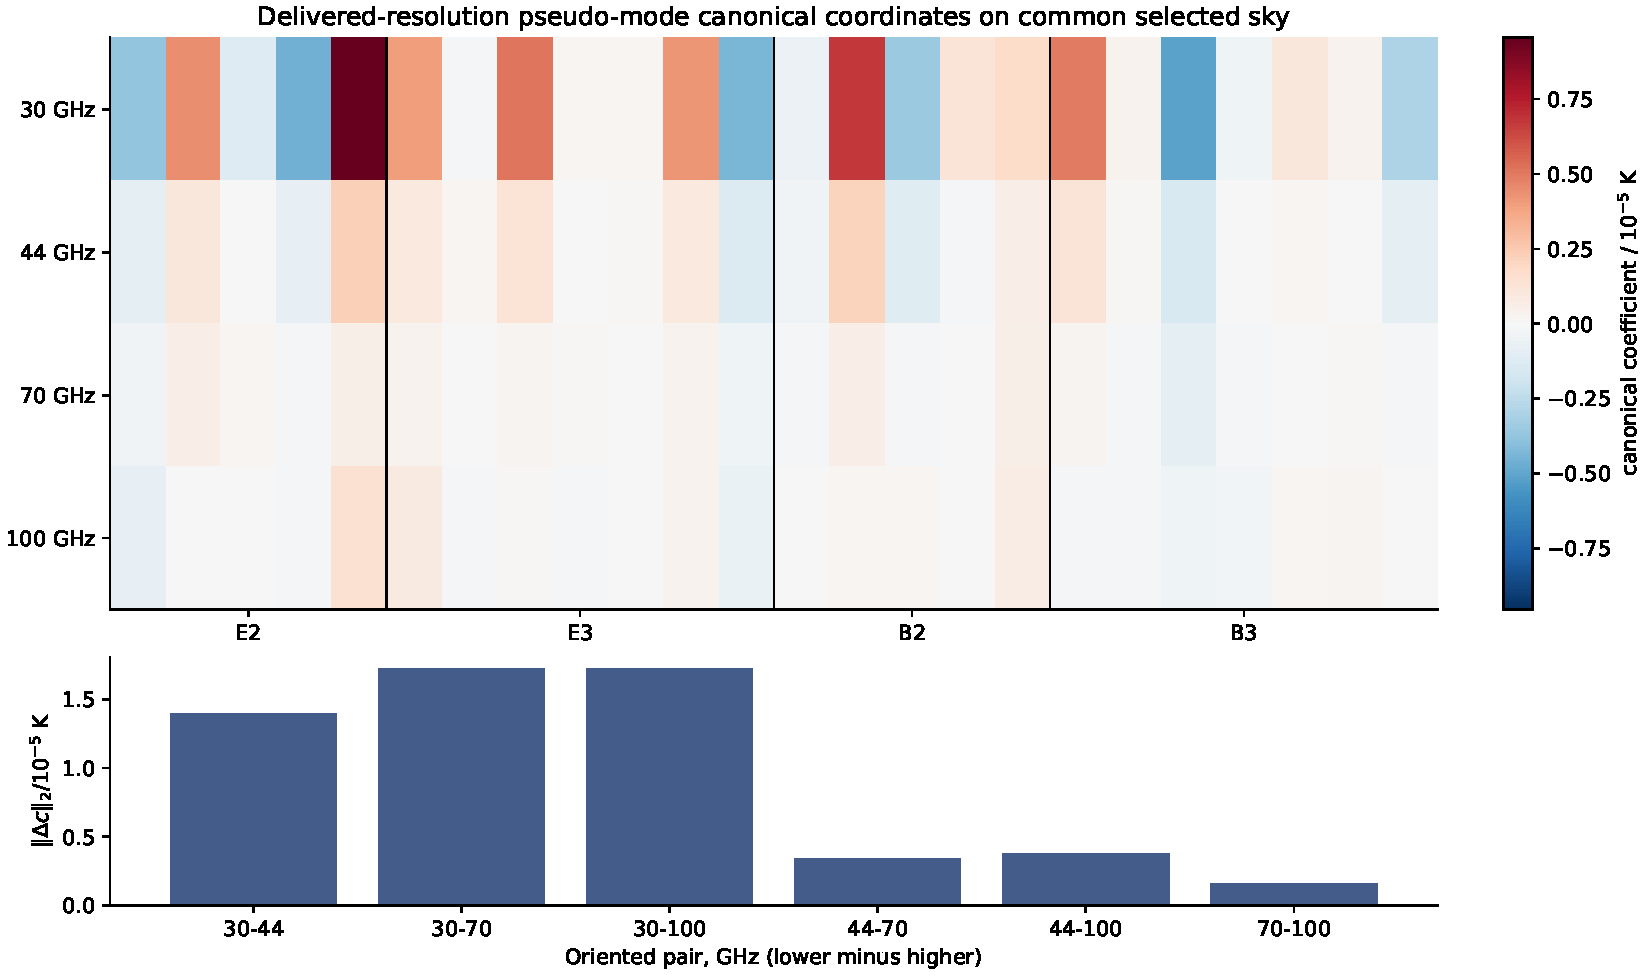
\includegraphics[width=\linewidth,height=.71\textheight,keepaspectratio]{figures/f104_external.pdf}
\caption{Complete quadrupole and octupole E/B pseudo-harmonic coordinates at four delivered frequencies and all six full-coordinate contrast norms. A common selected sky is used without map downgrading or deconvolution. Delivered beams, foregrounds, and mask leakage remain. These descriptive tensors do not supply a physical null, a frequency-to-depth map, or a completed seven-frequency result.}
\label{fig:f104}
\end{figure}
\clearpage
